\documentclass[openany]{ctexbook}

\usepackage{amsmath}
\usepackage{amssymb}
\usepackage{mathrsfs} %定义了类似铜版体的\mathscr
\usepackage{upgreek}
%\usepackage{textcomp}
\usepackage{xparse,physics}
\usepackage{cancel}
\usepackage{geometry}
\usepackage{booktabs}
\usepackage{array}
\usepackage{tabularx}
\usepackage{xcolor}
\usepackage{graphicx}
\usepackage{enumitem}
%\usepackage{fancyvrb}%能用颜文字卖萌了,2333
\usepackage{siunitx}%生成标准格式的国际单位
\usepackage{tensor}
\usepackage{tikz}
\usepackage{listings}
\usepackage{fontspec}
%\usepackage{minted}
\usepackage{pifont}
\usepackage{bm}
\usepackage{lmodern}
\usepackage{anyfontsize}
\usepackage{babel}
\usepackage[backend=biber,backref=true,style=authoryear]{biblatex}
% \usepackage{csquotes}
\usepackage{hyperref}
\usepackage{pgfplots}
\pgfplotsset{compat=1.18}
\usepackage[listings]{tcolorbox}
\usepackage[amsmath,hyperref,thmmarks,framed]{ntheorem}
\usepackage{pdftexcmds}
\usepackage{catchfile}
\usepackage{ifluatex}
\usepackage{ifplatform}

%%%%%%%%%%%%%%%  biblatex v3.15a bug fixing  %%%%%%%%%%%%%
% \providetoggle{blx@lang@captions@english}
%%%%%%%%%%%%%%%%%%%%%%%%%%%%%%%%%%%%%%%%%%%%%%%%%%%%%%%%%%

\allowdisplaybreaks

\usetikzlibrary{arrows.meta}
\usetikzlibrary{decorations.pathreplacing}
\usetikzlibrary{decorations.pathmorphing}
\usetikzlibrary{3d}

\tcbuselibrary{skins,breakable}

% \setmonofont{DejaVuSansMono Nerd Font}
\ifwindows
	\newfontfamily\codefont{DejaVuSansMono Nerd Font}
\fi
\iflinux
	\newfontfamily\codefont{DejaVuSansMono}
\fi
\ifmacosx
	\newfontfamily\codefont{DejaVuSansMono Nerd Font}
\fi

\geometry{
	a4paper,
	centering,
	scale=0.77,
	showframe
}

\lstset{
	backgroundcolor=\color[gray]{0.95},
	basicstyle=\codefont,
	stringstyle=\sffamily,
	flexiblecolumns,
	escapechar='
}

\hypersetup{
	colorlinks=true,
	linkcolor=blue,
	pdftitle={梁灿彬《微分几何入门与广义相对论》习题参考解答},
	pdfauthor={薛定谔的大喵}
}

%\newtheorem{mytheorem}{定理}[chapter]

%\newenvironment{yuanli}{\begin{list}{}{%
%			\leftmargin=4em \itemindent=0pt %
%			\topsep=1em \rightmargin=4em %
%		}%
%		\item \itshape%
%	}{%
%	\end{list}\normalfont}

{
	\theoremstyle{nonumberplain}
	\theoremheaderfont{\normalfont\bfseries}
	\theorembodyfont{\normalfont\slshape}
	\theoremsymbol{\ensuremath{\diamondsuit}}
	\theoremseparator{.}
	% \theoremprework{\bigskip\hrule}
	% \theorempostwork{\hrule\bigskip}
	\newtheorem{Theorem}{定理}
}
{
	\theoremstyle{nonumberplain}
	\theoremheaderfont{\normalfont\bfseries}
	\theorembodyfont{\normalfont\ttfamily\small}
	% \theoremsymbol{\ensuremath{\diamondsuit}}
	\theoremseparator{}
	% \theoremprework{\bigskip\hrule}
	% \theorempostwork{\hrule\bigskip}
	\newtheorem{Proposition}{命题}
}
{
	\theoremstyle{nonumberplain}
	\theoremheaderfont{\normalfont\bfseries}
	\theorembodyfont{\normalfont\ttfamily\small}
	% \theoremsymbol{\ensuremath{\diamondsuit}}
	\theoremseparator{}
	% \theoremprework{\bigskip\hrule}
	% \theorempostwork{\hrule\bigskip}
	\newtheorem{Property}{性质}
}
{
	\theoremstyle{plain}
	\theorembodyfont{\normalfont\itshape\small}
	% \theoremsymbol{\ensuremath{\heartsuit}}
	% \theoremindent0.5cm
	% \theoremnumbering{greek}
	\newtheorem{Lemma}{引理}
}
{
	\theoremheaderfont{\normalfont\upshape\bfseries}
	\theorembodyfont{\normalfont\mdseries\ttfamily\small}
	\theoremstyle{nonumberplain}
	\theoremseparator{}
	\theoremsymbol{\mbox{$\square$}}
	\newtheorem{Proof}{证明}
}

\newcommand{\myvec}[1]{\vec{#1}} %定制矢量格式
\newcommand{\myvu}[1]{\vu*{#1}}%单位矢量
%\providecommand{\dd}[0]{\mathrm{d}}
\newcommand{\e}[1]{\mathrm{e}^{#1}}
\newcommand{\dvt}[2][]{\dv[#1]{#2}{t}}
\newcommand{\pdvt}[2][]{\pdv[#1]{#2}{t}}
\newcommand{\pd}[1]{\pdv*{}{#1}}
\newcommand{\liej}[1]{\ensuremath{{#1}_1,\cdots,{#1}_n}}
\newcommand{\qqiff}{\qq{iff}}
\newcommand{\F}{\ensuremath{\mathscr{F}}}
\newcommand{\La}{\ensuremath{\mathscr{L}}}
\newcommand{\Ld}[1]{\ensuremath{\mathcal{L}}\indices{_{#1}}}
\newcommand{\TT}{\ensuremath{\mathscr{T}}}
\newcommand{\inner}[1]{\mathrm{i}\left( #1 \right)}
\newcommand{\ii}{\mathrm{i}}
\newcommand{\I}{\ensuremath{\mathrm{I}}}
\newcommand{\J}{\ensuremath{\mathrm{J}}}
\newcommand{\hj}[2][-1bp]{\raisebox{#1}{
\includegraphics[height=#2 bp]{pictures/hj}}}
\newcommand{\wl}[2][-1bp]{\raisebox{#1}{
\includegraphics[height=#2 bp]{pictures/wulian}}}
\newcommand{\Nabla}[1]{\tensor{\nabla}{_{#1}}}%协变导数算符
\newcommand{\tNabla}[1]{\tensor{{\tilde{\nabla}}}{_{#1}}}%另一个协变导数算符
\newcommand{\Partial}[1]{\tensor{\partial}{_{#1}}}%普通导数算符
\newcommand{\Fd}[2][\tau]{\ensuremath{\frac{\mathrm{D_F}#2}{\dd{#1}}}}%费米导数
\newcommand{\Fdd}[2][\tau]{\ensuremath{\mathrm{D_F}#2/\dd{#1}}}%行内费米导数
\newcommand{\Dd}[2][\tau]{\ensuremath{\frac{\mathrm{D}#2}{\dd{#1}}}}%协变导数
\newcommand{\Ddd}[2][\tau]{\ensuremath{\mathrm{D}#2/\dd{#1}}}%行内协变导数
\newcommand{\ChristoffelSymbol}[3]{\tensor{\Gamma}{^{#1}_{#2}_{#3}}}
\newcommand{\christoffelSymbol}[4]{\frac{1}{2} \tensor{g}{^{#1}^{#4}} \left( \tensor{g}{_{#4}_{#2}_{,#3}} + \tensor{g}{_{#3}_{#4}_{,#2}} - \tensor{g}{_{#2}_{#3}_{,#4}} \right) }
\newcommand{\riemannR}[5]{\tensor{\Gamma}{^{#4}_{#1}_{#3}_{,#2}}- \tensor{\Gamma}{^{#4}_{#2}_{#3}_{,#1}}+ \ChristoffelSymbol{#5}{#3}{#1} \ChristoffelSymbol{#4}{#2}{#5}- \ChristoffelSymbol{#5}{#3}{#2} \ChristoffelSymbol{#4}{#1}{#5}}
\newcolumntype{Y}{>{\centering\arraybackslash}X}
\newcommand{\tmu}{\mspace{2mu}}
\newcommand{\mmacs}{\bfseries\codefont\itshape\color[RGB]{67,137,88}}%mma局部变量字体
\newcommand{\mmab}{\bfseries\codefont\color[RGB]{60,125,145}}%mma变量字体
\newcommand{\mmaundef}{\bfseries\codefont\color[RGB]{0,44,195}}%mma未定义
\newcommand{\mma}{\bfseries\codefont}%mma代码字体
\newcommand{\myarrow}{-{Latex[length=5pt 6,width'=0pt 0.3]}}
\newcommand{\SO}[1]{\ensuremath{\mathrm{SO}\left(#1\right)}}
\newcommand{\OO}[1]{\ensuremath{\mathrm{O}\left(#1\right)}}

\newcommand{\form}[1]{\bm{#1}}

\newcommand{\tensord}[2]{\tensor{\left( \dd{#1} \right)}{_{#2}}}
\newcommand{\tensorp}[2]{\tensor{\left( \pdv{#1} \right)}{^{#2}}}

\newcommand{\TB}[2][{}]{\mathrm{T}_{#1}\!{#2}}
\newcommand{\TBx}[2][{}]{\mathrm{T}_{#1} {#2}}
\newcommand{\CTB}[2][{}]{\mathrm{T}^*_{#1}\!{#2}}

\renewcommand{\CancelColor}{\color{blue!70!red}}

\newcommand*{\circled}[1]{\lower.7ex\hbox{\tikz\draw (0pt, 0pt)circle (.5em) node {\makebox[1em][c]{\small #1}};}}

\newenvironment{jianjie}[1][2em]{%
\heiti\chapter*{说明}\begin{list}{}{%
\itemindent=#1 \listparindent=2em%
\leftmargin=2em \rightmargin=2em%
\parsep=0pt}\kaishu\item }{\end{list}}

\DeclareMathOperator{\ddiv}{div}
\DeclareMathOperator{\ggrad}{grad}
\DeclareMathOperator{\ccurl}{curl}
\DeclareMathOperator{\Exp}{Exp}

\title{《微分几何入门与广义相对论》\\部分习题参考解答}
\author{by 薛定谔的大喵\thanks{\href{mailto:wyj1234@mail.ustc.edu.cn}{wyj1234@mail.ustc.edu.cn}}}

\addbibresource{ref.bib}

\includeonly{chapters/c9}

\begin{document}
	\newcounter{xiti}[chapter]
\setcounter{xiti}{0}
\newcounter{subxiti}[xiti]
\setcounter{subxiti}{0}
\renewcommand{\thesubxiti}{\alph{subxiti}}
%\renewcommand{\thexiti}{\arabic{xiti}}
%\newcommand{\xit}{\stepcounter{xiti}\ensuremath{\mathbf{\thexiti}}\ }

\newenvironment{xiti}[1][0em]{%
\heiti\section*{习题}\begin{list}{\stepcounter{xiti}\textbf{\thexiti .}}{%
\itemindent=#1 \listparindent=\itemindent%
\leftmargin=0em \rightmargin=0pt%
\parsep=0pt}\normalfont}{\end{list}}

%\newenvironment{subxiti}{%
%\begin{list}{\stepcounter{subxiti}\textbf{(\thesubxiti)}}{\itemindent=0em \listparindent=2em%
%\parsep=0em \leftmargin=2em \rightmargin=0em}%
%\itemsep=0em \topsep=0em \parskip=0em%
%}{\end{list}}

\newenvironment{zm}{%
\begin{list}{\textbf{证明}}{%
\itemindent=0em \listparindent=2em%
\leftmargin=2.5em \rightmargin=0em%
\parsep=0pt \labelwidth=2em}\item \kaishu}{ \end{list}}
		
\newenvironment{jie}{%
\begin{list}{\textbf{解}}{%
\itemindent=0em \listparindent=2em%
\leftmargin=2em \rightmargin=0em%
\parsep=0pt \labelwidth=1em}\item \kaishu}{\end{list}}

\newenvironment{da}{%
\begin{list}{\textbf{答}}{%
\itemindent=0em \listparindent=2em%
\leftmargin=2em \rightmargin=0em%
\parsep=0pt \labelwidth=1em}\item \kaishu}{\end{list}}

\newenvironment{yl}[1]{%
\begin{list}{\textbf{#1}}{%
\itemindent=0em \listparindent=2em%
\leftmargin=2em \rightmargin=1em%
\parsep=0pt \labelwidth=3em}\item }{ \end{list}}
	\maketitle

	% \begin{jianjie}
	% 	本文档虽今天重新编译生成,但是内容是我数月前初学时所写,所有习题解答没有多次复核,仅供参考。若有错误之处请多多谅解,也可与我联系指出。

	% 	前五章是18年寒假时所写,之后春季学期断断续续写了些后面的,第六章所需作图很多,当时我尚未熟悉使用 Ti\textit{k}Z 作图,感到比较吃力,后来就鸽了……之后读其他章节时陆续写了点。

	% 	我一向觉得初学一个领域需要一些练习的积累,而苦于很多书上的练习题没有解答,做来又不知道对不对。梁先生的《微分几何入门与广义相对论》三卷在中文教材中可谓精品,我很希望梁书能流行起来,希望我以后能有空将这份答案补全(Flag立下……)

	% 	\vspace{12pt}
	% 	\begin{tabularx}{0.8\textwidth}{cXc}
	% 		&&薛定谔的大喵\\
	% 		&&\itshape 2018.11.3
	% 	\end{tabularx}
	% \end{jianjie}

	\frontmatter

	\tableofcontents

	\mainmatter

	\part{上册}
	% !TeX root = ../document.tex

\chapter{拓扑空间简简介}

\begin{xiti}
	\item 试证$\displaystyle A-B=A\cap (X-B)$,$\displaystyle \forall A,B\subset X$。
	
	\begin{zm}
			$  x\in A-B \iff x\in A \wedge x\notin B\iff x\in A\cap (X-B) $。 
	\end{zm}
	
	\item 试证$X-(B-A)=(X-B)\cup A$,$ \forall A,B\subset X$。
	
	\begin{zm}
		$ x\in X-(B-A) \iff x\notin B-A \iff x\notin B \vee x\in A \iff x\in (X-B)\cup A $。
	\end{zm}
	
	\item 用“对”或“错”在下表中填空:
	\begin{table}[htb]
		\begin{tabularx}{\textwidth}{YYY}
			\toprule
			$f\colon \mathbb{R}\rightarrow \mathbb{R} $&是一一的&是到上的\\
			\midrule
			$f(x)=x^3 $& & \\
			$f(x)=x^2$& &\\
			$f(x)=\e{x}$&&\\
			$f(x)=\cos x$&&\\
			$f(x)=5,\forall x\in \mathbb{R}$&&\\
			\bottomrule
		\end{tabularx}
	\end{table}
	
	\begin{jie}
		如下表:
		\begin{table}[htb]
			\begin{tabularx}{\textwidth}{YYY}
				\toprule
				$f\colon \mathbb{R}\rightarrow \mathbb{R} $&是一一的&是到上的\\
				\midrule
				$f(x)=x^3$&\textit{对} &\textit{对}\\
				$f(x)=x^2 $&\textit{错} &\textit{错}\\
				$f(x)=\e{x}$&\textit{对}&\textit{错}\\
				$f(x)=\cos x$&\textit{错}&\textit{错}\\
				$f(x)=5,\forall x\in \mathbb{R}$&\textit{错}&\textit{错}\\
				\bottomrule
			\end{tabularx}
		\end{table}
	\end{jie}
	
	\item 判断下列说法的是非并简述理由:
	\begin{enumerate}
		\item[(a)] 正切函数是由$\mathbb{R}$到$\mathbb{R}$的映射;
		\item[(b)] 对数函数是由$\mathbb{R}$到$\mathbb{R}$的映射;
		\item[(c)] $\left(a,b\right]\subset \mathbb{R}$用$\TT_u$衡量是开集;
		\item[(d)] $\left[a,b\right]\subset \mathbb{R}$用$\TT_u$衡量是闭集。
	\end{enumerate}
	
	\begin{jie}
		\begin{enumerate}
			\item[(a)] 错,定义域不是$\mathbb{R}$;
			\item[(b)] 错,定义域不是$\mathbb{R}$;
			\item[(c)] 错,任意包含于$\left(a,b\right]$的开区间都不会含有$b$,故$\left(a,b\right]$不能写为开区间之并;
			\item[(d)] 对,其补集$(-\infty,a)\cup (b,\infty)$是开集。
		\end{enumerate}
	\end{jie}

	
	\item 举一反例证明命题“$\left(\mathbb{R},\TT_u\right)$的无限个开子集之交为开“不真。
	
	\begin{zm}
		记$\displaystyle O_n=\left(-\frac{1}{n},\frac{1}{n}\right)$,则$\displaystyle\bigcap_{n=1}^{\infty} O_n=\{0\}$为闭集。
	\end{zm}
	
	\item 试证\S 1.2例5中定义的诱导拓扑满足定义1的3个条件。
	
	\begin{zm}
		拓扑空间$(X,\TT)$的子集$A$上的诱导拓扑按照定义为
		$$ \mathscr{S}:=\left\{ V\subset A\mid \exists O\in \TT, \qq{s.t.}V=A\cap O \right\}, $$
		\begin{enumerate}
			\item[(a)] $A,\varnothing \in \mathscr{S}$:取$O=X$即知$A\in\mathscr{S}$,取$O=\varnothing$即知$A\in \mathscr{S}$;
			\item[(b)] 有限交:设$V_i=A\cap O_i\in \mathscr{S}$,其中$O_i\in\TT $,$i=1,2,\cdots,n$。则
			\begin{equation*}
			\bigcap_{i=1}^n V_i =A\cap \left(\bigcap_{i=1}^n O_i \right)\in \mathscr{S};
			\end{equation*}
			\item[(c)] 无限并:设$V_\alpha=A\cap O_\alpha \in \mathscr{S}$,其中$O_\alpha\in\TT $,$\alpha\in \text{某个指标集} I$。则
			\begin{equation*}
			\bigcup_{\alpha\in I} V_\alpha =A\cap \left(\bigcup_{\alpha\in I} O_\alpha \right)\in \mathscr{S}.
			\end{equation*}
		\end{enumerate}
	\end{zm}

	\item 举例说明$(\mathbb{R}^3,\TT_u)$中存在不开不闭的子集。
	
	\begin{jie}
		令$A=\left(0,1 \right]^3 $,任何包含于$A$的开球$B_{r}(x_0,y_0,z_0) $的$z$坐标的范围为开区间$(z_0-r,z_0+r)\in (0,1]$,故$(x,y,1)$不能属于此开球,于是$A$不能由一族开球之并得到,故$A$不是开集。其补集中$(x,y,0)$不能属于开球,故补集不是开集,故$A$不是闭集。
	\end{jie}
	
	\item \hypertarget{1.8}{} 常值映射$f\colon \left(X,\TT\right)\rightarrow\left(Y,\mathscr{S}\right) $是否连续?为什么?
	
	\begin{jie}
		连续。证明如下:设$f[X]=\{y\}\subset Y$,$\forall O\in \mathscr{S} $,若$y\in O$,则$f^{-1}[O]=X\in \TT$;若$y\notin O$,则$f^{-1}[O]=\varnothing \in\TT $。故$f$连续。
	\end{jie}

	\item 设$\TT$为集$X$上的离散拓扑,$\mathscr{S}$为集$Y$上的凝聚拓扑,
	\begin{enumerate}
		\item[(a)] 找出从$\left(X,\TT\right)$到$\left(Y,\mathscr{S}\right)$的全部连续映射;
		\item[(b)] 找出从$\left(Y,\mathscr{S}\right)$到$\left(X,\mathscr{T}\right)$的全部连续映射。
	\end{enumerate}
	
	\begin{jie}
		\begin{enumerate}
			\item[(a)] 设$f\colon X\rightarrow Y$,则由于$\mathscr{S}=\{Y,\varnothing\}$,$f$连续当且仅当$f^{-1}[Y]=X\in \TT \wedge f^{-1}[\varnothing]=\varnothing\in \TT$,可是这是必然满足的,于是所有映射$f\colon \left(X,\TT\right)\rightarrow\left(Y,\mathscr{S}\right) $均连续。
			\item[(b)] 设$g\colon Y\rightarrow X$,则由于$\mathscr{T}=2^X$,$g$连续当且仅当$\forall O\subset X $,$g^{-1}[O]=X \vee g^{-1}[O]=\varnothing $。假设存在$x,y\in g[Y]$,$x\neq y$,则取$O={x} $,有$g^{-1}[O]=g^[-1](x)\notin \mathscr{S} $,故$g$不是连续的。于是连续映射$g$的像只能有一个,即为常值映射。又~\hyperlink{1.8}{8}~中已证明常值映射为连续,故$g\colon \left(Y,\mathscr{S}\right)\rightarrow\left(X,\TT\right) $连续当且仅当其为常值映射。
		\end{enumerate}
	\end{jie}
	
	\item 试证明定义3a与3b的等价性。
	
	\begin{zm}
		\begin{enumerate}
			\item[(1)] 3a推导3b。设$f\colon \left(X,\TT \right)\rightarrow\left(Y,\mathscr{S}\right) $连续,按照定义3a即满足$\forall O\in\mathscr{S} $,$f^{-1}[O]\in\TT $。则$\forall x\in X$,任取$G^\prime\in\mathscr{S} $使得$f(x)\in G^\prime $,则只需取$G=f^{-1}[G^\prime] $,即有$G\in\TT $并且$f[G]=G^\prime \subset G^\prime $,于是按照定义3b,$f$也连续。
			\item[(2)] 3b推导3a。设$f\colon \left(X,\TT \right)\rightarrow\left(Y,\mathscr{S}\right) $连续,按照定义3b即满足$\forall x\in X $,$\forall G^\prime\in \mathscr{S} $且$f(x)\in G^\prime $,$\exists G\in \TT $使得$f[G]\subset G^\prime $。于是任取$O\in \mathscr{S} $,令$x$跑遍$f^{-1}[O]$,对每一个$x$存在$G_x\in \TT$使得$f[G_x]\subset O $,考虑$\displaystyle G=\bigcup_{x\in f^{-1}[O]} G_x $,显然$G\in\TT $。由于$x\in f^{-1}[O] $,$x\in G_x $因而$x\in G $,于是$f^{-1}[O]\subset G $;而$\forall x\in G $,不妨设$x\in G_{x_0}$,则由于$f[G_{x_0}]\subset O $,知$x\in f^{-1}[O] $,故又有$G\subset f^{-1}[O] $,于是$G$正是$f^{-1}[O] $,也就是$f^{-1}[O]=G\in \TT $,按照定义3a,$f$也是连续的。
			
		\end{enumerate}
	\end{zm}
	
	\item 试证任一开区间$(a,b)\subset \mathbb{R} $与$\mathbb{R} $同胚。
	
	\begin{zm}
		只需找到一个同胚映射。函数$f\colon (a,b)\rightarrow \mathbb{R} $定义为$\displaystyle f(x)=\tan(\pi\frac{x-a}{b-a}-\frac{\pi}{2}) $即满足要求。
	\end{zm}
	
	\item 设$X_1 $和$X_2$是$\mathbb{R}$的子集,$X_1\equiv(1,2)\cup(2,3) $,$X_2\equiv(1,2)\cup[2,3)$。以$\TT_1$和$\TT_2$分别代表由$\mathbb{R}$的通常拓扑在$X_1$和$X_2$上的诱导拓扑。拓扑空间$(X_1,\TT_1)$和$(X_2,\TT_2)$是否连通?
	
	\begin{jie}
		\begin{enumerate}
			\item[(1)] $(X_1,\TT_1) $不连通。考虑$O=(1,2)\subset X_1$,$O=X_1\cap (1,2)\in\TT_1 $,故$O$为开集;而$X-O=(2,3)$同样为开集,于是$O$即开又闭,故$(X_1,\TT_1)$不连通。
			\item[(2)] $(X_2,\TT_2)$连通。假设$\exists O\neq X_2 ,O\neq\varnothing$,$O\in \TT$且$X-O\in\TT_2$,任取$a\in O$,$b\in X-O$,不妨设$a<b$,于是$[a,b]\subset X_2 $,记$A=[a,b]\cap O$,$B=[a,b]\cap (X-O) $,$c=\sup A$,我们来证明$O$和$X-O$都是开集将导致$c\notin A$并且$c\notin (X-O)$,从而矛盾。
			\begin{enumerate}
				\item \hypertarget{1.12.2.a}{}若$c\in B$,由于$X-O$是开集,且由于$X_2=(1,3)\in\TT_u \implies \TT_2=\TT_u\cap 2^{X_2}$,$X-O$可以写作一系列开区间之并,于是$B=(X-O)\cap[a,b]$是一系列形如$[a,y),(x,y)$或$(x,b]$的区间之并,现在$c\neq a$,故包含$c$的区间属后两种,则一定存在$d\in B$,使$(d,c]\subset B$,
				\begin{enumerate}
					\item 若$c=b$,则$(d,b]\subset B$;
					\item 若$a<c<b$,则$(d,b]=(d,c]\cup(c,b]\subset B $,
				\end{enumerate}
			    于是$d$是$A$的上界,然而却小于上确界$c$,矛盾。
			    \item 若$c\in A$,同\hyperlink{1.12.2.a}{(a)}有$O$是开集将导致$\exists e\in A$,使得$[c,e)\subset A$,与$c$是$A$的上确界矛盾。
			\end{enumerate}
		    至此$c\in A$与$c\in B$均导致矛盾,然而$c\notin A \wedge c\notin B$又与$A$和$B$的定义矛盾,故$O$与$X-O$均为非空开集是不可能的。故${X_2,\TT_2}$连通。
		\end{enumerate}
	\end{jie}
	
	\item 任意集合$X$配以离散拓扑$\TT$所得的拓扑空间是否连通?
	
	\begin{jie}
		不连通。$\forall O\in X $,$O\in \TT \wedge X-O\in\TT \implies X\text{不连通}$。
	\end{jie}
	
	\item 设$A\subset B$,试证
	\begin{enumerate}
		\item[(a)] $\bar{A}\subset\bar{B}$;提示:$A\subset B$表明$\bar{B}$是含$A$的闭集。
		\item[(b)] $\mathrm{i}(A)\subset \mathrm{i}(B)$。
	\end{enumerate}
	
	\begin{zm}
		\begin{enumerate}
			\item[(a)] $A\subset B\subset\bar{B} $,根据闭包定义有$\bar{A}\subset\bar{B} $;
			\item[(b)] $\ii{A}\subset A\subset B $,根据内部定义有$\ii{A}\subset \ii{B} $。
		\end{enumerate}
	\end{zm}
	
	\item 试证$x\in \bar{A}\iff x $的任一邻域与$A$之交非空。对$\implies$证明的提示:设$O\in \TT$且$O\cap A=\varnothing$,先证$A\subset X-O$,再证(利用闭包定义)$\bar{A}\subset X-O$。
	
	\begin{zm}
		\begin{enumerate}
			\item[(1)] $\implies$:不妨设$O$是$x$的开邻域。假设$O\cap A=\varnothing$,于是$\forall a\in A$,$a\neq A $,于是$a\in X-O$,$A\subset X-O$,而$X-O$为闭集,于是$\bar{A}\subset X-O$,故知$x\notin\bar{A} $,矛盾;
			\item[(2)] $\impliedby$:设$\forall O\in \TT$使得$x\in O$,都有$O\cap A\neq \varnothing$。假设$x\notin \bar{A}$,根据定义,$\exists B$为闭集,$A\subset B$且$x\notin B$。于是$x\in X-B \in\TT$,于是$X-B$是$x$的一个与$A$无交的开邻域,矛盾。
		\end{enumerate}
	\end{zm}
	
	\item 试证$\mathbb{R}$不是紧致的。
	
	\begin{zm}
		记$O_i=(i-1,i+1)$,显然$\{O_i\}_{i\in\mathbb{Z}}$是$\mathbb{R}$的开覆盖。现挑出其中任意$n$个$O_{i_k}\qc k=1,2,\cdots,n$,则$\displaystyle\max_{k=1,2,\cdots,n} i_k+1$即为$\displaystyle\bigcup_{k=1,2,\cdots,n}O_{i_k} $的一个上界,故有限个元素不能覆盖$\mathbb{R}$,于是$\mathbb{R}$不是紧致的。
	\end{zm}
	
	
	
	
	
	
	
	
	
\end{xiti}
	% !TeX root = ../document.tex

\chapter{流形和张量场}
\begin{xiti}
	\item 试证 \S 2.1例2定义的拓扑同胚映射$\psi_i^{\pm}$在$O_i^{\pm}$的所有交叠区域上满足相容性条件,从而证实$S^1$确是1维流形。

	\begin{zm}
		首先,易知$O_i^+ \cap O_i^- =\varnothing$,故只需考虑$O_1^+\cap O_2^+ $及$O_i^+ \cap O_j^- $。
		以$$O_1^+ \cap O_2^+ =\left\lbrace \left(x^1,x^2\right)\in S^1 \mid x^1>0,x^2>0 \right\rbrace  $$为例,根据定义,
		\begin{equation*}
		\psi_2^+ \circ \left(\psi_1^+\right)^{-1}(t)=\psi_2^+\left(\left(\sqrt{1-t^2},t\right)\right)=\sqrt{1-t^2},
		\end{equation*}
		这的确是$C^\infty$的函数。
	\end{zm}

	\item 说明$n$维矢量空间可看作$n$维平庸流形。

	\begin{zm}
		为$n$维矢量空间$V$任取拓扑,再取定一组基$\mathcal{B}= \{ e_i \}_{i=1}^n $ ,则在基$\mathcal{B}$下,$\forall v \in V$,$v$可展开为
		\begin{equation*}
		v=\sum_{i=1}^{n} v^i e_i,
		\end{equation*}
		令映射$\psi \colon V\rightarrow \mathbb{R}^n$定义为:
		\begin{equation*}
		\psi\colon v\mapsto\left(v^1,v^2,\cdots,v^n\right),
		\end{equation*}
		则取图册$\{(V,\psi)\} $,即可令$V$成为$n$维平庸流形。
	\end{zm}

    \item 设$X$和$Y$是拓扑空间,$f\colon X\rightarrow Y$是同胚。若$X$还是个流形,试给$Y$定义一个微分结构使$f\colon X\rightarrow Y$升格为微分同胚。
    \begin{zm}
    	记$X$的图册为$\left\{ \left(O_\alpha,\psi_\alpha\right) \right\}$,对每个$\alpha$,由于$f$是拓扑同胚,$$O_{\alpha}^{\prime}:=f(O_{\alpha})\in \TT_Y,$$在$O_\alpha^\prime$上定义映射$$\psi_\alpha^\prime:=\psi_\alpha\circ f^{-1},$$则
    	\begin{equation*}
    	\begin{split}
    	\psi_\alpha^{\prime}\circ f\circ \psi_\alpha^{-1} &=\psi_\alpha\circ f^{-1} \circ f \circ \psi_\alpha^{-1}\\
    	&=\operatorname{Id}_{V_\alpha}\in C^\infty(V_\alpha),
    	\end{split}
    	\end{equation*}
    	 于是在给$Y$定义图册$\{(O_\alpha^{\prime} ,\psi_\alpha^{\prime})\} $后,$f$成为一个微分同胚。
    \end{zm}

    \item 设$(x,y)$是$\mathbb{R}^2$的自然坐标,$C(t)$是曲线,参数表达式为$x=\cos t,\quad y=\sin t,\quad t\in (0,\pi)$。若$p=C(\pi/3)$,写出曲线在$p$的切矢在自然坐标基的分量,并画图表示出该曲线及该切矢。

    \begin{jie}
    	记$p$点切矢为$T$,则
    	\begin{align*}
    	T_x&=\eval{\dv{t}(x\circ C(t))}_{t=\frac{\pi}{3}}=-\frac{\sqrt{3}}{2}\\
    	T_y&=\eval{\dv{t}(y\circ C(t))}_{t=\frac{\pi}{3}}=\frac{1}{2}
    	\end{align*}
    	如下图:
    	\begin{figure}[htb]
    		\centering
    		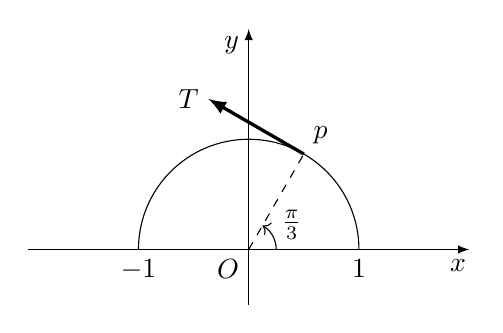
\begin{tikzpicture}[scale=0.7]
    		\draw[-latex] (-4,0) -- (4,0);
    		\draw[-latex] (0,-1) -- (0,4);
    		\draw (2,0) arc (0:180:2);
    		\node[below left] (O) at (0,0) {$O$};
    		\node[below] (x) at (3.8,0) {$x$};
    		\node[left] (y) at (0,3.7) {$y$};
    		\node[below] (r) at (2,0) {$1$};
    		\node[below] (rr) at (-2,0) {$-1$};
    		\coordinate[label=above right:$p$] (p) at (60:2);
    		\coordinate[label=left:$T$] (T) at (-0.732,2.732);
    		\draw[very thick,-latex] (p) -- (T);
    		\draw[dashed] (0,0) -- (p);
    		\draw[->] (0.5,0) arc (0:60:0.5);
    		\node (j) at (30:0.9) {$\frac{\pi}{3}$};
    		\end{tikzpicture}
    		\caption{曲线$C(t)$及其在$p$点的切矢}
    	\end{figure}
    \end{jie}

    \item 设曲线$C(t)$和$C^{\prime}(t)\equiv C(2t_0-t) $在$ C(t_0)=C^\prime(t_0) $点的切矢分别为$v$和$v^\prime$,试证$v+v^\prime=0$。

    \begin{zm}
    	记$t^\prime=2t_0-t$,依定义,$\forall f\in \F_M$,
    	\begin{equation*}
    	\begin{split}
    	v(f)&=\eval{\dv{(f\circ C(t))}{t}}_{t=t_0},\\
    	v^\prime(f)&=\eval{\dv{(f\circ C^{\prime}(t))}{t}}_{t=t_0}\\
    	&=\eval{\dv{(f\circ C(t^{\prime}))}{t}}_{t=t_0}\\
    	&=\eval{\dv{t^{\prime}}{t}}_{t=t_0} \times \eval{\dv{(f\circ C(t^{\prime}))}{t^{\prime}}}_{t=t_0,\text{即}t^{\prime}=2t_0-t=t_0}\\
    	&=-\eval{\dv{(f\circ C(t^{\prime}))}{t^{\prime}}}_{t^{\prime}=t_0}\\
    	&=-v(f)
    	\end{split}
    	\end{equation*}
    	$\therefore v^{\prime}=-v,\quad v+v^{\prime}=0$
    \end{zm}

    \item 设$O$为坐标系$\{x^{\mu}\}$的坐标域,$p\in O$,$v\in V_p$,$v^\mu$是$v$的坐标分量,把坐标$x^\mu$看作$O$上的$C^\infty$函数,试证$v^\mu=v(x^\mu)$。提示:用$v=v^\nu X_\nu $两边作用于函数$x^\mu$。

    \begin{zm}
    	由$v=v^\nu X_\nu$,
    	\begin{equation*}
    	v(x^\mu)=v^\nu X_\nu(x^\mu)=v^\nu \eval{\pdv{x^\mu}{x^\nu}}_p=v^\nu \tensor{\delta}{^\mu_\nu}=v^\mu.
    	\end{equation*}
    \end{zm}

    \item 设$M$是二维流形,$(O,\psi)$和$(O^\prime,\psi^\prime)$是$M$上的两个坐标系,坐标分别为$\{x,y\}$和$\{x^\prime,y^\prime\}$,在$O\cap O^\prime$上的坐标变换为$x^\prime=x\qc y^\prime=y-\Omega x(\Omega=\text{常数})$,试分别写出坐标基矢$\pd{x},\pd{y}$用坐标基矢$\pd{x^\prime},\pd{y^\prime}$的展开式。

    \begin{jie}
    	坐标基矢逐点的变换关系为$\displaystyle  X_\mu=\eval{\pdv{x^{\prime\nu}}{x^\mu}}_p X_\nu $,故
    	\begin{equation*}
    	\begin{split}
    	\pdv{x}&=\pdv{x^\prime}{x}\pdv{x^\prime}+\pdv{y^\prime}{x}\pdv{y^\prime}\\
    	&=\pdv{x^\prime}-\Omega\pdv{y^\prime};\\
    	\pdv{y}&=\pdv{x^\prime}{y}\pdv{x^\prime}+\pdv{y^\prime}{y}\pdv{y^\prime}\\
    	&=\pdv{y^\prime}.
    	\end{split}
    	\end{equation*}
    \end{jie}

    \item \begin{enumerate}
    	\item[(a)] 试证式(2-2-9)的$[u,v]$在每点满足矢量定义(\S2.2定义2)的两个条件,从而的确是矢量场。
    	\item[(b)] 设$u,v,w$为流形$M$上的光滑矢量场,试证$$ \left[\left[u,v\right],w\right]+\left[\left[w,u\right],v\right]+\left[\left[v,w\right],u\right]=0 $$\hypertarget{ykb}{}(此式称为\textbf{雅可比恒等式})。
    \end{enumerate}

    \begin{zm}
    	\begin{enumerate}
    		\item[(a)]
    		\begin{enumerate}
    			\item[(i)] 线性性:显然;
    			\item[(ii)] 莱布尼兹律:显然。证毕\footnote{皮这一下非常开心\textasciitilde \hj{11}}。
    		\end{enumerate}
    	    \item[(b)] 由定义,逐次展开有:
    	    \begin{equation*}
    	    \begin{split}
    	    &[[u,v],w]+[[w,u],v]+[[v,w],u]\\
    	    =&\;[u,v]\circ w-w \circ [u,v]+[w,u]\circ v\\
    	    &-v \circ [w,u]+[v,w]\circ u -u\circ [v,w]\\
    	    =&\;u\circ v\circ w-v\circ u\circ w-w\circ u\circ v+w\circ v\circ u\\
    	    &+w\circ u\circ v-u\circ w\circ v-v\circ w\circ u+v\circ u\circ w\\
    	    &+v\circ w\circ u-w\circ v\circ u-u\circ v\circ w+u\circ w\circ v\\
    	    =&\;0.
    	    \end{split}
    	    \end{equation*}
    	\end{enumerate}
    \end{zm}

    \item 设$\{r,\phi\}$为$\mathbb{R}^n$中某开集(坐标域)上的极坐标,$\{x,y\}$为自然坐标,
    \begin{enumerate}
    	\item[(a)] 写出极坐标系的坐标基矢$\pd{r}$和$\pd{\phi}$(作为坐标域上的矢量场)用$\pd{x},\ \pd{y}$展开的表达式。
    	\item[(b)] 求矢量场$[\pd{r},\pd{x}]$用$\pd{x},\pd{y}$展开的表达式。
    	\item[(c)] 令$\hat{e}_r\equiv\pd{r},\hat{e}_\phi=r^{-1}\pd{\phi}$,求$[\hat{e}_r,\hat{e}_\phi]$用$\pd{x},\pd{y}$展开的表达式。
    \end{enumerate}

    \begin{jie}
    	\begin{enumerate}
    		\item[(a)] 坐标变换为
    		\begin{equation*}
    		\Bigg\{
    		\begin{aligned}
    		x&=r \cos \phi,\\
    		y&=r \sin \phi.
    		\end{aligned}
    		\Bigg.
    		\end{equation*}
    		于是
    		\begin{align*}
    		\allowdisplaybreaks
    		\pdv{r}&=\pdv{x}{r}\pdv{x}+\pdv{y}{r}\pdv{y}\\
    		&=\cos \phi \pdv{x}+\sin \phi \pdv{y}\\
    		&=\frac{x}{\sqrt{x^2+y^2}} \pdv{x}+\frac{y}{\sqrt{x^2+y^2}}\pdv{y},\\
    		\pdv{\phi}&=\pdv{x}{\phi}\pdv{\phi}+\pdv{y}{\phi}\pdv{\phi}\\
    		&=-r\sin \phi \pdv{x}+r\cos \phi \pdv{y}\\
    		&=-y\pdv{x}+x\pdv{y}.
    		\end{align*}
    		\item[(b)] $\forall f\in \F_M,$
    		\begin{align*}
    		\allowdisplaybreaks
    		\left[\pdv{r},\pdv{x}\right](f)=&\;\left(\frac{x}{\sqrt{x^2+y^2}}\pdv{x}+\frac{y}{\sqrt{x^2+y^2}}\pdv{y}\right)\pdv{x}(f)\\
    		&-\pdv{x}\left(\frac{x}{\sqrt{x^2+y^2}}\pdv{x}+\frac{y}{\sqrt{x^2+y^2}}\pdv{y}\right)(f)\\
    		=&\;\frac{x}{\sqrt{x^2+y^2}}\pdv[2]{F}{x}+\frac{y}{\sqrt{x^2+y^2}}\pdv{F}{y}{x}\\
    		&-\pdv{x}(\frac{x}{\sqrt{x^2+y^2}}\pdv{F}{x})-\pdv{x}(\frac{y}{\sqrt{x^2+y^2}}\pdv{F}{y})\\
    		=&-\pdv{x}(\frac{x}{\sqrt{x^2+y^2}})\pdv{F}{x}-\pdv{x}(\frac{y}{\sqrt{x^2+y^2}})\pdv{F}{y}\\
    		=&-\frac{y^2}{\left(x^2+y^2\right)^{\frac{3}{2}}}\pdv{F}{x}+\frac{x y}{\left(x^2+y^2\right)^\frac{3}{2}}\pdv{F}{y}\\
    		=&\;\left(-\frac{y^2}{\left(x^2+y^2\right)^\frac{3}{2}}\pdv{x}+\frac{x y}{\left(x^2+y^2\right)^\frac{3}{2}}\pdv{y}\right)(f),
    		\end{align*}
    		$\therefore $在基$\pdv{x},\pdv{y}$下,
    		\begin{equation*}
    		\left[\pdv{r},\pdv{x}\right]=-\frac{y^2}{\left(x^2+y^2\right)^\frac{3}{2}}\pdv{x}+\frac{x y}{\left(x^2+y^2\right)^\frac{3}{2}}\pdv{y}.
    		\end{equation*}
    		\item[(c)] 由(a),
    		\begin{align*}
    		\hat{e}_r&=\pdv{r}=\frac{x}{\sqrt{x^2+y^2}}\pdv{x}+\frac{y}{\sqrt{x^2+y^2}}\pdv{y},\\
    		\hat{e}_\phi&=\frac{1}{r}\pdv{\phi}=-\frac{y}{\sqrt{x^2+y^2}}\pdv{x}+\frac{x}{\sqrt{x^2+y^2}}\pdv{y},
    		\end{align*}
    		于是有$\forall f\in \F_M$,
    		\begin{align*}
    		\allowdisplaybreaks
    		&\;[\hat{e}_r,\hat{e}_\phi](f)\\
    		=&\;\left(\frac{x}{\sqrt{x^2+y^2}}\pdv{x}+\frac{y}{\sqrt{x^2+y^2}}\pdv{y}\right)\left(-\frac{y}{\sqrt{x^2+y^2}}\pdv{x}+\frac{x}{\sqrt{x^2+y^2}}\pdv{y}\right)(f)\\\displaybreak[2]
    		&-\left(-\frac{y}{\sqrt{x^2+y^2}}\pdv{x}+\frac{x}{\sqrt{x^2+y^2}}\pdv{y}\right)\left(\frac{x}{\sqrt{x^2+y^2}}\pdv{x}+\frac{y}{\sqrt{x^2+y^2}}\pdv{y}\right)(f)\\
    		=&\;\frac{x}{\sqrt{x^2+y^2}}\pdv{x}(-\frac{y}{\sqrt{x^2+y^2}}\pdv{F}{x})+\frac{x}{\sqrt{x^2+y^2}}\pdv{x}(\frac{x}{\sqrt{x^2+y^2}}\pdv{F}{y})\\
    		&+\frac{y}{\sqrt{x^2+y^2}}\pdv{y}(-\frac{y}{\sqrt{x^2+y^2}}\pdv{F}{x})+\frac{y}{\sqrt{x^2+y^2}}\pdv{y}(\frac{x}{\sqrt{x^2+y^2}}\pdv{F}{y})\\
    		&+\frac{y}{\sqrt{x^2+y^2}}\pdv{x}(\frac{x}{\sqrt{x^2+y^2}}\pdv{F}{x})+\frac{y}{\sqrt{x^2+y^2}}\pdv{x}(\frac{y}{\sqrt{x^2+y^2}}\pdv{F}{y})\\
    		&-\frac{x}{\sqrt{x^2+y^2}}\pdv{y}(\frac{x}{\sqrt{x^2+y^2}}\pdv{F}{x})-\frac{x}{\sqrt{x^2+y^2}}\pdv{y}(\frac{y}{\sqrt{x^2+y^2}}\pdv{F}{y})\\
    		=&-\frac{x}{\sqrt{x^2+y^2}}\pdv{x}(\frac{y}{\sqrt{x^2+y^2}})\pdv{F}{x}-\cancel{\frac{xy}{x^2+y^2}\pdv[2]{F}{x}}\\
    		&+\frac{x}{\sqrt{x^2+y^2}}\pdv{x}(\frac{x}{\sqrt{x^2+y^2}})\pdv{F}{y}+\cancel{\frac{x^2}{x^2+y^2}\pdv{F}{x}{y}}\\
    		&-\frac{y}{\sqrt{x^2+y^2}}\pdv{y}(\frac{y}{\sqrt{x^2+y^2}})\pdv{F}{x}-\cancel{\frac{y^2}{x^2+y^2}\pdv{F}{y}{x}}\\
    		&+\frac{y}{\sqrt{x^2+y^2}}\pdv{y}(\frac{x}{\sqrt{x^2+y^2}})\pdv{F}{y}+\cancel{\frac{xy}{x^2+y^2}\pdv[2]{F}{y}}\\
    		&+\frac{y}{\sqrt{x^2+y^2}}\pdv{x}(\frac{x}{\sqrt{x^2+y^2}})\pdv{F}{x}+\cancel{\frac{xy}{x^2+y^2}\pdv[2]{F}{x}}\\
    		&+\frac{y}{\sqrt{x^2+y^2}}\pdv{x}(\frac{y}{\sqrt{x^2+y^2}})\pdv{F}{y}+\cancel{\frac{y^2}{x^2+y^2}\pdv{F}{y}{x}}\\
    		&-\frac{x}{\sqrt{x^2+y^2}}\pdv{y}(\frac{x}{\sqrt{x^2+y^2}})\pdv{F}{x}-\cancel{\frac{x^2}{x^2+y^2}\pdv{F}{y}{x}}\\
    		&-\frac{x}{\sqrt{x^2+y^2}}\pdv{y}(\frac{y}{\sqrt{x^2+y^2}})\pdv{F}{y}-\cancel{\frac{xy}{x^2+y^2}\pdv[2]{F}{y}}
    		\end{align*}
    		……好了算到这里我受够了,我选择直接丢进Mathematica让麦酱来算\heiti{( ̄$\upomega$ ̄;)}\kaishu 麦酱报告说结果是酱紫:
    		\begin{equation*}
    		\frac{y}{x^2+y^2}\pdv{F}{x}-\frac{x}{x^2+y^2}\pdv{F}{y}
    		\end{equation*}
    		于是得到
    		\begin{equation*}
    		[\hat{e}_r,\hat{e}_\phi]=\frac{y}{x^2+y^2}\pdv{x}-\frac{x}{x^2+y^2}\pdv{y}
    		\end{equation*}
    	\end{enumerate}
    \end{jie}

    \item 设$u$,$v$为$M$上的矢量场,试证$[u,v]$在任何坐标基底的分量满足$$[u,v]^\mu = v^\nu \pdv*{v^\mu}{x^\nu}-v^\nu \pdv*{u^\mu}{x^\nu} .\quad \text{提示:用式(2-2-$3'$)和(2-2-3)} $$

    \begin{zm}
    	$\forall f \in \F_M$,
    	\begin{align*}
    	[u,v](f)=&\;\left[u^\mu \pdv{x^\mu} ,v^\nu \pdv{x^\nu} \right](f)\\
    	=&\;u^\mu \pdv{x^\mu}(v^\nu \pdv{F}{x^\nu})-v^\nu \pdv{x^\nu}(u^\mu \pdv{F}{x^\nu})\\
    	=&\;u^\mu \pdv{v^\nu}{x^\mu} \pdv{F}{x^\nu}-v^\nu \pdv{u^\mu}{x^\nu}\pdv{F}{x^\mu}\\
    	=&\;\left(u^\nu \pdv{v^\mu}{x^\nu}-v^\nu \pdv{u^\mu}{x^\nu} \right)\pdv{F}{x^\mu}
    	\end{align*}
    	故
    	\begin{align*}
    	&[u,v]=\left(u^\nu \pdv{v^\mu}{x^\nu}-v^\nu \pdv{u^\mu}{x^\nu} \right)\pdv{x^\mu},\\
    	&[u,v]^\mu=\left(u^\nu \pdv{v^\mu}{x^\nu}-v^\nu \pdv{u^\mu}{x^\nu} \right).
    	\end{align*}
    \end{zm}

    \item 设$\{e_{\mu}\}$为$V$的基底,$\{e^{\mu*}\}$为其对偶基底,$v\in V$,$\omega\in V^*$,试证$$ \omega=\omega(e_\mu)e^{\mu*}\qc v=e^{\mu*}(v)e_\mu. $$

    \begin{zm}
    	设$\omega=\tensor{\omega}{_\mu} e^{\mu *}$,则
    	\begin{align*}
    	\omega(e_\nu)=&\;\tensor{\omega}{_\mu} e^{\mu*}(e_\nu)\\
    	=&\;\tensor{\omega}{_\mu} \tensor{\delta}{^{\mu}_\nu}\\
    	=&\;\tensor{\omega}{_\nu},
    	\end{align*}
    	$\therefore \omega=\omega(e_\mu)e^{\mu*}.$同理设$v=v^\mu e_\mu $,
    	\begin{align*}
    	e^{\nu*}(v)=&\; v^\mu e^{\nu*}(e_\mu)\\
    	=&\; v^\mu \tensor{\delta}{^\nu_\mu}\\
    	=&\; v^\nu,
    	\end{align*}
    	$\therefore v=e^{\mu*}e_\mu .$
    \end{zm}

    \item 试证$\displaystyle\tensor{{\omega^\prime}}{_\mu} =\pdv{x^\mu}{x^{\prime \nu}} \tensor{\omega}{_\mu} $(定理2-3-4)。

    \begin{zm}
    	由上题,
    	\begin{align*}
    	\allowdisplaybreaks
    	\tensor{{\omega^\prime}}{_\nu} &= \omega\left(\pdv{x^{\prime\nu}}\right)\\
    	\displaybreak[1]
    	&=\omega\left(\pdv{x^\mu}{x^{\prime\nu}}\pdv{x^\mu}\right)\\
    	\displaybreak[1]
    	&=\pdv{x^\mu}{x^{\prime\nu}}\omega\left(\pdv{x^\mu}\right)\\
    	\displaybreak[1]
    	&=\pdv{x^\mu}{x^{\prime\nu}}\tensor{\omega}{_\mu}.
    	\end{align*}
    \end{zm}

    \item 试证由式(2-3-5)定义的映射$v\mapsto v^{**}$是同构映射。提示:可利用线性代数的结论,即同维矢量空间之间的一一线性映射必到上。

    \begin{zm}
    	留作习题答案略,读者自证不难(逃$-\!=\equiv $Σ(((つ \!\!\! •̀ω$\upomega$•́) \!\!\! つ)
    \end{zm}

    \item 设$C^1_1 T$和$(C^1_1 T)^\prime$分别是$(2,1)$型张量$T$借两个基底$\{e_\mu\}$和$\{ {e^\prime}_\mu \}$定义的缩并,试证$\left(C_1^1 T\right)^{\prime}=C_1^1 T$。

    \begin{zm}
    	记基$ \{{e^\prime}_\mu \} $在基$\{e_\mu \}$下的展开式为${e^\prime}_\mu = \tensor{A}{^{\nu}_{\mu}}e_\nu $ ,则$${e^\prime}^{\mu*}=\tensor{\left(\tilde{A}^{-1} \right)}{_{\nu}^{\mu} } e^{\nu *} ,$$于是$\forall \omega\in V^* $,
    	\begin{align*}
    	\left(C_1^1 T\right)^\prime (\omega)=&\;  T({e^\prime}^{\mu*},\omega;{e^\prime}_\mu)\\
    	=&\; T\left(\tensor{\left(\tilde{A}^{-1} \right)}{_{\nu}^{\mu} } e^{\nu*},\omega;\tensor{A}{ ^{\sigma}_{\mu} } e_{\sigma} \right)\\
    	=&\;\tensor{\left(\tilde{A}^{-1} \right)}{_{\nu}^{\mu} } \tensor{A}{^{\sigma}_{\mu}} T\left( e^{\nu*},\omega;e_\sigma \right)\\
    	=&\;\tensor{\left(\tilde{A}^{-1} \right)}{_{\nu}^{\mu} } \tensor{\left( \tilde{A} \right)}{ _{\mu}^{\sigma} } T(e^{\nu*},\omega;e_\sigma)\\
    	=&\; \tensor{\delta}{_{\nu}^{\sigma}} T(e^{\nu*},\omega;e_\sigma)\\
    	=&\; T(e^{\nu*},\omega;e_\nu)\\
    	=&\; C_1^1 T(\omega).
    	\end{align*}
    \end{zm}

    \item 设$g$为$V$的度规,试证$ g\colon V\rightarrow V^* $是同构映射(可参见第13题的提示)。

    \begin{zm}
    	线性空间的同构映射指的是可逆线性映射。这里证一个更普遍的结论,首先我们定义一个线性映射$T\colon V\rightarrow W $的kernel为$$ \ker T:=\{ v\in V\mid T(v)=0 \}, $$我们有如下claim:
    	\begin{yl}{claim}
    		$T$是单射当且仅当$\ker T=\{0\}$。
    	\end{yl}
        \begin{yl}{proof}
        	若$T$是单射,由于$\forall v\in V$,$T(0\cdot v)=0T(v)=0\qc \therefore \ker T=\{0\} $;
        	若$\ker T=\{0\}$,假设存在$u,v\in V$,使得$T(u)=T(v)$,则由于$T$是线性映射,$T(u-v)=T(u)-T(v)=0$,于是$u-v \in \ker T $,即$u=v $,于是$T$是单射。
        \end{yl}
        易证任取一组基$e_i\in V $, $T(e_i)\in W$线性无关当且仅当$\ker T=\{0\} $,若$\dim V=\dim W $,则这告诉我们$T(e_i) $构成$W$的基,于是$T(v^i e_i)=v^i T(e_i)$将取遍整个$W$。于是我们证明了,若$\dim V=\dim W$,则线性映射$T\colon V\rightarrow W$为一一到上的(等价于可逆)当且仅当$\ker T=\{0\}$。

        对于度规$g$,由于非退化性,知$\ker g=\{0\}$,故$g$为线性同构。
    \end{zm}

    \item 试证线长与曲线的参数化无关。

    \begin{zm}
    	设有重参数化$C^\prime(t^\prime)=C(t)$,线长为
    	\begin{align*}
    	\allowdisplaybreaks
    	l^\prime=&\;\int_{\alpha^\prime}^{\beta^\prime} \sqrt{\tensor{g}{_\mu_\nu} \dv{x^\mu}{t^\prime}\dv{x^\nu}{t^\prime} }\dd{t^\prime}\\
    	=&\;\int_{\alpha}^{\beta} \sqrt{\tensor{g}{_\mu_\nu} \left(\dv{t}{t^\prime}\dvt{x^\mu} \right)\left( \dv{t}{t^\prime}\dvt{x^\nu} \right) }\left| \dvt{t^\prime} \right|\dd{t}\\
    	=&\;\int_{\alpha}^{\beta} \sqrt{\tensor{g}{_\mu_\nu}\dvt{x^\mu}\dvt{x^\nu} }\dd{t}\\
    	=&\;l.
    	\end{align*}
    \end{zm}

    \item 设$(x,y)$是二维欧氏空间的笛卡尔坐标系,试证由式(2-5-14)定义的$\{x^\prime,y^\prime \}$也是笛卡尔系。

    \begin{zm}
    	式(2-5-14)为
    	\begin{equation*}
    	\left\{
    	\begin{aligned}
    	x^\prime &=x \cos \alpha +y \sin \alpha,\\
    	y^\prime&=-x \sin \alpha+y \cos \alpha.
    	\end{aligned}
    	\right.
    	\end{equation*}
    	其逆为:
    	\begin{displaymath}
    	\left\{
    	\begin{aligned}
    	x=x^\prime \cos \alpha-y^\prime \sin \alpha,\\
    	y=x^\prime \sin \alpha+y^\prime \cos \alpha.
    	\end{aligned}\right.
    	\end{displaymath}
    	于是坐标基矢的变换为:
    	\begin{align*}
    	\pdv{x^\prime}=&\;\pdv{x}{x^\prime}\pdv{x}+\pdv{y}{x^\prime}\pdv{y}\\
    	=&\;\cos \alpha \pdv{x}+\sin \alpha \pdv{y},\\
    	\pdv{y^\prime}=&\;\pdv{x}{y^\prime}\pdv{x}+\pdv{y}{y^\prime}\pdv{y}\\
    	=&-\sin \alpha \pdv{x}+\cos \alpha \pdv{y}.
    	\end{align*}
    	故
    	\begin{align*}
    	\displaybreak[1]
    	\delta\left( \pdv{x^\prime},\pdv{x^\prime} \right)=&\tmu\cos^2 \alpha\ \delta\left(\pdv{x},\pdv{x}\right)+2\cos \alpha \sin \alpha\ \delta \left(\pdv{x},\pdv{y}\right)\\
    	&+\sin^2 \alpha\ \delta \left(\pdv{y},\pdv{y}\right) \\
    	\displaybreak[1]=&\;1;\\
    	\delta\left(\pdv{y^\prime},\pdv{y^\prime}\right)=&\tmu\sin^2 \alpha\ \delta\left(\pdv{x},\pdv{x}\right)-2\cos \alpha \sin \alpha\ \delta \left(\pdv{x},\pdv{y}\right)\\
    	&\mspace{1mu}+\cos^2 \alpha\ \delta \left(\pdv{y},\pdv{y}\right) \\
    	\displaybreak[1]=&\;1;\\
    	\delta\left(\pdv{x^\prime},\pdv{y^\prime}\right)=&\;\delta\left(\pdv{y^\prime},\pdv{x^\prime}\right)\\
    	=&\mspace{1mu}-\mspace{-1mu}\cos \alpha \sin \alpha\ \delta\left(\pdv{x},\pdv{x}\right)+\cos 2\alpha\ \delta\left( \pdv{x},\pdv{y} \right)\\
    	&\mspace{1mu}+\cos \alpha \sin \alpha\ \delta\left(\pdv{y},\pdv{y}\right)\\
    	=&\;0.
    	\end{align*}
    	$\therefore \{x^\prime,y^\prime\}$是笛卡尔系。
    \end{zm}

    \item 设$\{t,x\}$是二维闵氏空间的洛伦兹坐标系,试证由式(2-5-20)定义的$\left\{t^\prime,x^\prime \right\}$也是洛伦兹系。

    \begin{zm}
    	式(2-5-20)为
    	\begin{equation*}
    	\left\{
    	\begin{aligned}
    	t^\prime &=t \cosh \lambda +x \sinh \lambda,\\
    	x^\prime&=t \sinh \lambda+x \cosh \lambda.
    	\end{aligned}
    	\right.
    	\end{equation*}
    	其逆为:
    	\begin{displaymath}
    	\left\{
    	\begin{aligned}
    	t&=t^\prime \cosh \lambda-x^\prime \sinh \lambda,\\
    	x&=-t^\prime \sinh \lambda+x^\prime \cosh \lambda.
    	\end{aligned}\right.
    	\end{displaymath}
    	于是坐标基矢的变换为:
    	\begin{align*}
    	\pdv{t^\prime}=&\;\pdv{t}{t^\prime}\pdv{t}+\pdv{x}{t^\prime}\pdv{x}\\
    	=&\tmu\cosh \lambda \pdv{t}-\sinh \lambda \pdv{x},\\
    	\pdv{x^\prime}=&\;\pdv{t}{x^\prime}\pdv{t}+\pdv{x}{x^\prime}\pdv{x}\\
    	=&\mspace{1mu}-\mspace{-1mu}\sinh \lambda \pdv{t}+\cosh \lambda \pdv{x}.
    	\end{align*}
    	故
    	\begin{align*}
    	\eta \left( \pdv{t^\prime},\pdv{t^\prime} \right)=&\tmu\cosh^2 \lambda\ \eta\left(\pdv{t},\pdv{t}\right)-2\cosh \lambda \sinh \lambda\ \eta \left(\pdv{t},\pdv{x}\right)\\
    	&+\sinh^2 \lambda\ \eta \left(\pdv{x},\pdv{x}\right) \\
    	\displaybreak[1]=&\mspace{1mu}-\mspace{-4mu}1;\\
    	\eta\left(\pdv{x^\prime},\pdv{x^\prime}\right)=&\tmu\sinh^2 \lambda\ \eta\left(\pdv{t},\pdv{t}\right)-2\cosh \lambda \sinh \lambda\ \eta \left(\pdv{t},\pdv{x}\right)\\
    	&+\cosh^2 \lambda\ \eta \left(\pdv{x},\pdv{x}\right) \\
    	\displaybreak[1]=&\;1;\\
    	\eta\left(\pdv{t^\prime},\pdv{x^\prime}\right)=&\;\eta\left(\pdv{x^\prime},\pdv{t^\prime}\right)\\
    	=&\mspace{1mu}-\mspace{-1mu}\cosh \lambda \sinh \lambda\ \eta\left(\pdv{t},\pdv{t}\right)+\cosh 2\lambda\ \eta\left(\pdv{t},\pdv{x}\right)\\
    	&-\cosh \lambda \sinh \lambda\ \eta\left(\pdv{x},\pdv{x}\right)\\
    	=&\;0.
    	\end{align*}
    	$\therefore \{t^\prime,x^\prime\}$是洛伦兹系。
    \end{zm}

    \item \begin{enumerate}
    	\item[(a)] \hypertarget{2.19a}{} 用张量变换律求出3维欧氏度规在球坐标系中的全部分量$\tensor{{g^\prime}}{_{\mu\nu}}$。
    	\item[(b)] 已知4维闵氏度规$g$在洛伦兹系中的线元表达式为$\dd{s}^2=-\dd{t}^2+\dd{x}^2+\dd{y}^2+\dd{z}^2 $,求$g$及其逆$g^{-1}$在新坐标系$\{t^\prime,x^\prime,y^\prime,z^\prime\}$的全部分量$\tensor{{g^\prime}}{_{\mu\nu}}$以及$\tensor{{g^\prime}}{^{\mu\nu}} $,该新坐标系定义如下:
    	\begin{gather*}
    	t^\prime=t\qc z^\prime=z\qc x^\prime=(x^2+y^2)^{1/2}\cos(\phi-\omega t),\\
    	y^\prime=(x^2+y^2)^{1/2}\sin(\phi-\omega t)\qc \omega=\text{常数},
    	\end{gather*}
    	其中$\phi$满足$\cos \phi=y(x^2+y^2)^{1/2}\qc \sin \phi=x(x^2+y^2)^{1/2}$。提示:先求$\tensor{{g^\prime}}{_{\mu\nu}}$再求$\tensor{{g^\prime}}{^{\mu\nu}}$。
    \end{enumerate}

    \begin{jie}
    	\begin{enumerate}
    		\item[(a)] 球坐标与笛卡尔系的变换关系为:
    		\begin{displaymath}
    		\left\{
    		\begin{aligned}
    		x&=r\sin \theta \cos \phi,\\
    		y&=r\sin \theta \sin \phi,\\
    		z&=r\cos \theta.
    		\end{aligned}
    		\right.
    		\end{displaymath}
    		则
    		\begin{align*}
    		\tensor{{g^\prime}}{_{rr}}&=\pdv{x^\mu}{r}\pdv{x^\nu}{r} \tensor{g}{_{\mu\nu}}\\
    		&=\left(\sin \theta \cos \phi \right)^2+\left( \sin \theta \sin \phi \right)^2+\cos^2 \theta\\
    		\displaybreak[1]&=1;\\
    		\tensor{{g^\prime}}{_{r\theta}}&=\pdv{x^\mu}{r}\pdv{x^\nu}{\theta} \tensor{g}{_{\mu\nu}}\\
    		&=\sin \theta\cos\phi\cdot r\cos\theta\cos\phi+\sin\theta\sin\phi\cdot r\cos\theta\sin\phi-\cos\theta\cdot r\sin\theta\\
    		\displaybreak[1]&=0;\\
    		\tensor{{g^\prime}}{_{r\phi}}&=\pdv{x^\mu}{r}\pdv{x^\nu}{\phi} \tensor{g}{_{\mu\nu}}\\
    		&=-\sin\theta\cos\phi\cdot r\sin\theta\sin\phi+\sin\theta\sin\phi\cdot r\sin\theta\cos\phi+0\\
    		\displaybreak[1]&=0;\\
    		\tensor{{g^\prime}}{_{\theta\theta}}&=\pdv{x^\mu}{\theta}\pdv{x^\nu}{\theta} \tensor{g}{_{\mu\nu}}\\
    		&=(r\cos\theta\cos\phi)^2+(r\cos\theta\sin\phi)^2+(-r\sin\theta)^2\\
    		\displaybreak[1]&=r^2;\\
    		\tensor{{g^\prime}}{_{\theta\phi}}&=\pdv{x^\mu}{\theta}\pdv{x^\nu}{\phi} \tensor{g}{_{\mu\nu}}\\
    		&=-r\cos\theta\cos\phi\cdot r\sin\theta\sin\phi+r\cos\theta\sin\phi\cdot r\sin\theta\cos\phi+0\\
    		\displaybreak[1]&=0;\\
    		\tensor{{g^\prime}}{_{\phi\phi}}&=\pdv{x^\mu}{\phi}\pdv{x^\nu}{\phi} \tensor{g}{_{\mu\nu}}\\
    		&=(-r\sin\theta\sin\phi)^2+(r\sin\theta\cos\phi)^2+0\\
    		&=r^2\sin^2\theta.
    		\end{align*}
    		\item[(b)] 先求偏导数:
    		\begin{gather*}
    		\displaybreak[1]
    		\sin \phi=\frac{x}{\sqrt{x^2+y^2}}\\\displaybreak[1]
    		\implies \cos \phi \dd{\phi}=\frac{y^2}{\left(x^2+y^2\right)^{\frac{3}{2}}}\dd{x}-\frac{xy}{\left(x^2+y^2\right)^{\frac{3}{2}}}\dd{y}\\
    		\displaybreak[1]
    		\implies \frac{y}{\sqrt{x^2+y^2}}\dd{\phi}=\frac{y^2}{\left(x^2+y^2\right)^{\frac{3}{2}}}\dd{x}-\frac{xy}{\left(x^2+y^2\right)^{\frac{3}{2}}}\dd{y}\\
    		\implies \pdv{\phi}{x}=\frac{y}{x^2+y^2} \qc \pdv{\phi}{y}=-\frac{x}{x^2+y^2}.
    		\end{gather*}
    		进而有:
    		\begin{align*}
    		\displaybreak[1]
    		\pdv{x^\prime}{t}&=\omega\sqrt{x^2+y^2}\sin(\phi-\omega t)\\
    		\pdv{x^\prime}{x}&=\frac{x}{\sqrt{x^2+y^2}}\cos(\phi-\omega t)-\sqrt{x^2+y^2}\sin(\phi-\omega t)\pdv{\phi}{x}\\
    		&=\frac{x}{\sqrt{x^2+y^2}}\cos(\phi-\omega t)-\frac{y}{\sqrt{x^2+y^2}}\sin(\phi-\omega t)\\
    		&=\frac{x}{x^2+y^2}\left( y\cos\omega t+x\sin\omega t \right)-\frac{y}{x^2+y^2}(x\cos\omega t-y\sin\omega t)\\\displaybreak[1]
    		&=\sin\omega t\\
    		\pdv{x^\prime}{y}&=\frac{y}{\sqrt{x^2+y^2}}\cos(\phi-\omega t)-\sqrt{x^2+y^2}\sin(\phi-\omega t)\pdv{\phi}{y}\\
    		&=\frac{y}{\sqrt{x^2+y^2}}\cos(\phi-\omega t)+\frac{x}{\sqrt{x^2+y^2}}\sin(\phi-\omega t)\\
    		&=\frac{y}{x^2+y^2}\left( y\cos\omega t+x\sin\omega t \right)+\frac{x}{x^2+y^2}(x\cos\omega t-y\sin\omega t)\\\displaybreak[1]
    		&=\cos\omega t\\\displaybreak[1]
    		\pdv{y^\prime}{t}&=-\omega\sqrt{x^2+y^2}\cos(\phi-\omega t)\\
    		\pdv{y^\prime}{x}&=\frac{x}{\sqrt{x^2+y^2}}\sin(\phi-\omega t)+\sqrt{x^2+y^2}\cos(\phi-\omega t)\pdv{\phi}{x}\\
    		&=\frac{x}{\sqrt{x^2+y^2}}\sin(\phi-\omega t)+\frac{y}{\sqrt{x^2+y^2}}\cos(\phi-\omega t)\\
    		&=\frac{x}{x^2+y^2}(x\cos\omega t-y\sin\omega t)+\frac{y}{x^2+y^2}(y\cos\omega t+x\sin\omega t)\\\displaybreak[1]
    		&=\cos\omega t\\
    		\pdv{y^\prime}{y}&=\frac{y}{\sqrt{x^2+y^2}}\sin(\phi-\omega t)+\sqrt{x^2+y^2}\cos(\phi-\omega t)\pdv{\phi}{y}\\
    		&=\frac{y}{\sqrt{x^2+y^2}}\sin(\phi-\omega t)-\frac{x}{\sqrt{x^2+y^2}}\sin(\phi-\omega t)\\
    		&=\frac{y}{x^2+y^2}(x\cos\omega t-y\sin\omega t)-\frac{x}{x^2+y^2}(y\cos\omega t+x\sin\omega t)\\
    		&=-\sin\omega t
    		\end{align*}
    		于是由张量变换律,
    		\begin{align*}
    		\tensor{{g^\prime}}{^{00}}=&\;\pdv{t^\prime}{x^\mu}\pdv{t^\prime}{x^\nu}\tensor{g}{^{\mu\nu}}\\
    		=&\mspace{1mu}-\mspace{-4mu}1^2+0^2+0^2+0^2\\\displaybreak[1]
    		=&\mspace{1mu}-\mspace{-4mu}1\\
    		\tensor{{g^\prime}}{^{01}}=&\;\pdv{t^\prime}{x^\mu}\pdv{x^\prime}{x^\nu}\tensor{g}{^{\mu\nu}}\\\displaybreak[1]
    		=&\mspace{1mu}-\mspace{-4mu}1\cdot \omega\sqrt{x^2+y^2}\sin(\phi-\omega t)+0+0+0\\\displaybreak[1]
    		=&\mspace{1mu}-\mspace{-4mu}\omega\sqrt{x^2+y^2}\sin(\phi-\omega t)\\\displaybreak[1]
    		\tensor{{g^\prime}}{^{02}}=&\;\pdv{t^\prime}{x^\mu}\pdv{y^\prime}{x^\nu}\tensor{g}{^{\mu\nu}}\\\displaybreak[1]
    		=&\mspace{1mu}-\mspace{-4mu}1\cdot \left(-\omega\sqrt{x^2+y^2}\cos(\phi-\omega t)\right)+0+0+0\\\displaybreak[1]
    		=&\;\omega\sqrt{x^2+y^2}\cos(\phi-\omega t)\\
    		\tensor{{g^\prime}}{^{03}}=&\;\pdv{t^\prime}{x^\mu}\pdv{z^\prime}{x^\nu}\tensor{g}{^{\mu\nu}}\\
    		=&\mspace{1mu}-\mspace{-4mu}0+0+0+0\\\displaybreak[1]
    		=&\;0\\
    		\tensor{{g^\prime}}{^{11}}=&\;\pdv{x^\prime}{x^\mu}\pdv{x^\prime}{x^\nu}\tensor{g}{^{\mu\nu}}\\
    		=&\mspace{1mu}-\mspace{-1mu}\left(\omega\sqrt{x^2+y^2}\sin(\phi-\omega t) \right)^2+\left(\sin\omega t \right)^2+\left(\cos\omega t\right)^2+0^2\\\displaybreak[1]
    		=&\;1-\left(x^2+y^2\right)\omega^2\sin[2](\phi-\omega t)\\
    		\tensor{{g^\prime}}{^{12}}=&\;\pdv{x^\prime}{x^\mu}\pdv{y^\prime}{x^\nu}\tensor{g}{^{\mu\nu}}\\
    		=&\mspace{1mu}-\mspace{-1mu}\left(\omega\sqrt{x^2+y^2}\sin(\phi-\omega t)\right)\cdot\left(-\omega\sqrt{x^2+y^2}\cos(\phi-\omega t)\right)\\&+\sin \omega t\cdot\cos\omega t+\cos\omega t\cdot\left(-\sin\omega t\right)+0\\\displaybreak[1]
    		=&\tmu\left(x^2+y^2\right)\omega^2\sin(\phi-\omega t)\cos(\phi-\omega t)\\
    		\tensor{{g^\prime}}{^{13}}=&\;\pdv{x^\prime}{x^\mu}\pdv{z^\prime}{x^\nu}\tensor{g}{^{\mu\nu}}\\
    		=&\mspace{1mu}-\mspace{-4mu}0+0+0+0\\\displaybreak[1]
    		=&\;0\\
    		\tensor{{g^\prime}}{^{22}}=&\;\pdv{y^\prime}{x^\mu}\pdv{y^\prime}{x^\nu}\tensor{g}{^{\mu\nu}}\\
    		=&\mspace{1mu}-\mspace{-1mu}\left(-\omega\sqrt{x^2+y^2}\cos(\phi-\omega t)\right)^2+\left(\cos\omega t\right)^2+\left(-\sin\omega t\right)^2+0^2\\\displaybreak[1]
    		=&\;1-\left(x^2+y^2\right)\omega^2\cos[2](\phi-\omega t)\\
    		\tensor{{g^\prime}}{^{23}}=&\;\pdv{y^\prime}{x^\mu}\pdv{z^\prime}{x^\nu}\tensor{g}{^{\mu\nu}}\\
    		=&\mspace{1mu}-\mspace{-4mu}0+0+0+0\\\displaybreak[1]
    		=&\;0\\
    		\tensor{{g^\prime}}{^{33}}=&\;\pdv{z^\prime}{x^\mu}\pdv{z^\prime}{x^\nu}\tensor{g}{^{\mu\nu}}\\
    		=&\mspace{1mu}-\mspace{-4mu}0^2+0^2+0^2+1^2\\
    		=&\;1.
    		\end{align*}
    		于是$g^{-1}$在带撇坐标系下的分量矩阵为:
    		\begin{displaymath}
    		\left[g^\prime\right]^{-1}=\left(
    		\begin{array}{cccc}
    		-1&-r\omega \sin\psi&r\omega \cos\psi&0\\
    		-r\omega \sin\psi&1-r^2\omega^2\sin^2 \psi&r^2\omega^2\sin\psi\cos\psi&0\\
    		-r\omega \sin\psi&r^2\omega^2\cos\psi\sin\psi&1-r^2\omega^2\cos^2\psi&0\\
    		0&0&0&1
    		\end{array}
    		\right),
    		\end{displaymath}
    		其中$r=\sqrt{x^2+y^2}$,$\psi=\phi-\omega t$。其逆矩阵为
    		\begin{displaymath}
    		\left[g^\prime\right]=\left(
    		\begin{array}{cccc}
    		r^2\omega^2-1&-r\omega \sin\psi&r\omega \cos\psi&0\\
    		-r\omega \sin\psi&1&0&0\\
    		r\omega \cos\psi&0&1&0\\
    		0&0&0&1
    		\end{array}
    		\right),
    		\end{displaymath}
    		此即$g$在带撇坐标系下的分量$\tensor{{g^\prime}}{_{\mu\nu}} $排成的矩阵。
    	\end{enumerate}
    \end{jie}

    \item 试证3维欧氏空间中球坐标基矢$\pd{r},\pd{\theta},\pd{\phi}$的长度依次为$1,r,	r\sin\theta$。

    \begin{zm}
    	由~\hyperlink{2.19a}{19(a)}~知,
    	\begin{align*}
    	\norm{\pdv{r}}&=\sqrt{\abs{\tensor{{g^\prime}}{_{rr}}}}=1,\\
    	\norm{\pdv{\theta}}&=\sqrt{\abs{\tensor{{g^\prime}}{_{\theta\theta}}}}=r,\\
    	\norm{\pdv{\phi}}&=\sqrt{\abs{\tensor{{g^\prime}}{_{\phi\phi}}}}=r\sin\theta.
    	\end{align*}
    \end{zm}

    \item 用抽象指标记号证明$\displaystyle\tensor{{T^\prime}}{^\mu_\nu}=\pdv{{x^\prime}^\mu}{x^\rho}\pdv{x^\sigma}{{x^\prime}^\nu}\tensor{T}{^\rho_\sigma} $。

    \begin{zm}
    	\begin{align*}
    	\tensor{{T^\prime}}{^\mu_\nu}=&\;\tensor{T}{^a_b}\tensor{\left(\dd{{x^\prime}^\mu}\right)}{_a}\left(\pdv{{x^\prime}^\nu}\right)^b\\
    	=&\;\tensor{T}{^a_b}\pdv{{x^\prime}^\mu}{x^\rho}\tensor{\left(\dd{{x^\prime}^\rho}\right)}{_a}\pdv{x^\sigma}{{x^\prime}^\nu}\left(\pdv{{x^\prime}^\sigma}\right)^b\\
    	=&\;\pdv{{x^\prime}^\mu}{x^\rho}\pdv{x^\sigma}{{x^\prime}^\nu}\tensor{T}{^\rho_\sigma}.
    	\end{align*}
    \end{zm}

    \item 以$g$和$g^\prime$分别代表度规$\tensor{g}{_{ab}}$在坐标系$\{x^\mu\}$和$\{{x^\prime}^\mu\}$的分量$\tensor{g}{_{\mu\nu}}$和$\tensor{{g^\prime}}{_{\mu\nu}}$组成的两个$n\times n$矩阵的行列式,试证$g^\prime=\abs{\pdv*{x^\rho}{{x^\prime}^\sigma}}^2 g$,其中$\abs{\pdv*{x^\rho}{{x^\prime}^\sigma}}$是坐标变换$\{x^\mu\}\mapsto \{{x^\prime}^\mu \} $的雅可比行列式,即由$\pdv*{x^\rho}{{x^\prime}^\sigma} $组成的$n\times n$行列式。注:本题表明度规的行列式在坐标变换下不是不变量。提示:取等式$\tensor{{g^\prime}}{_{\rho\sigma}}=\left( \pdv*{x^\mu}{{x^\prime}^\rho}\right)\left(\pdv*{x^\nu}{{x^\prime}^\sigma} \right)\tensor{g}{_{\mu\nu}}  $的行列式。

    \begin{zm}
    	……梁爷爷你提示都把题写完了我还写啥(˘•$\upomega$•˘)
    \end{zm}

    \item 设$\{x^\mu \}$是流形上的任一局域坐标系,试判断下列等式的是非:
    \begin{enumerate}
    	\item[(1)] $\left(\pd{x^\mu} \right)^a\tensor{\left(\pd{x^\nu} \right)}{_a}=\tensor{g}{_\mu_\nu} $,其中$\tensor{\left(\pd{x^\mu} \right)}{_a} \equiv \tensor{g}{_a_b}\left(\pd{x^\nu} \right)^a $;
    	\item[(2)] $\left(\dd{x^\mu}\right)^a\tensor{\left(\dd{x^\nu}\right)}{_a}=\tensor{g}{^\mu^\nu} $,其中$\left(\dd{x^\mu}\right)^a\equiv \tensor{g}{^a^b}\tensor{\left(\dd{x^\mu} \right)}{_b} $;
    	\item[(3)] \hypertarget{2.23.3}{}$\tensor{\left(\pd{x^\mu}\right)}{_a}=\tensor{\left(\dd{x^\mu} \right)}{_a} $;
    	\item[(4)] $\left(\dd{x^\mu} \right)^a=\tensor{{\left(\pd{x^\mu} \right)}}{^a} $;
    	\item[(5)] $v^\mu\tensor{\omega}{_\mu}=\tensor{v}{_\mu}\omega^\mu $;
    	\item[(6)] $\tensor{g}{_\mu_\nu}\tensor{T}{^\nu^\rho}\tensor{S}{_\rho^\sigma}=\tensor{T}{_\mu_\rho}\tensor{S}{^\rho^\sigma} $;
    	\item[(7)] $v^au^b=v^bu^a$;
    	\item[(8)] $v^au^b=u^bv^a$。
    \end{enumerate}

    \begin{jie}
    	\begin{enumerate}
    		\item[(1)] 正确。这是标量等式。根据(0,2)型张量分量的定义即知正确。
    		\item[(2)] 正确。这是标量等式。根据(2,0)型张量分量的定义即知正确。
    		\item[(3)] 不正确。这是对偶矢量等式。对其验证只需作用在坐标基矢上:
    		\begin{align*}
    		\tensor{\left(\pdv{x^\mu}\right)}{_a} \left(\pdv{x^\nu}\right)^a& =\tensor{g}{_\mu_\nu};\\
    		\tensor{\left(\dd{x^\mu}\right)}{_a}\left(\pdv{x^\nu}\right)^a& =\tensor{\delta}{_\mu_\nu},
    		\end{align*}
    		故 metric dual of basis 等于 dual basis 的条件为该坐标系是局域的笛卡尔系。
    		\item[(4)] 不正确。这是矢量等式。对其验证只需用对偶坐标基矢作用:
    		\begin{align*}
    		\tensor{\left(\dd{x^\mu}\right)}{^a}\tensor{\left(\dd{x^\nu}\right)}{_a} &=\tensor{g}{^\mu^\nu};\\
    		\tensor{\left(\pdv{x^\mu} \right)}{^a}\tensor{\left(\dd{x^\nu}\right)}{_a} &=\tensor{\delta}{^\mu^\nu}.
    		\end{align*}
    		故此式成立的条件为该坐标系为局域的笛卡尔系。或者可以这样得到:此式与~\hyperlink{2.23.3}{(3)}~中的表达式互为 metric dual,故它们是等价的。
    		\item[(5)] 正确。这是数量等式。
    		\begin{align*}
    		\tensor{v}{_\mu} \omega^\mu&=\tensor{g}{_\rho_\mu}v^\rho \tensor{g}{^\sigma^\mu}\omega_\mu\\
    		&=v^\rho \tensor{\omega}{_\rho}.
    		\end{align*}
    		\item[(6)] 正确。这是数量等式。
    		\begin{align*}
    		\tensor{g}{_\mu_\nu}\tensor{T}{^\nu^\rho}\tensor{S}{_\rho^\sigma}&=\tensor{g}{_\mu_\nu}\tensor{g}{^\nu^\alpha}\tensor{g}{^\rho^\beta}\tensor{T}{_\alpha_\beta}\tensor{g}{_\rho_\gamma}\tensor{S}{^\gamma^\sigma}\\
    		&=\tensor{\delta}{_\mu^\alpha}\tensor{\delta}{_\gamma^\beta}\tensor{T}{_\alpha_\beta}\tensor{S}{^\gamma^\sigma}\\
    		&=\tensor{T}{_\mu_\beta}\tensor{S}{^\beta^\sigma}.
    		\end{align*}
    		\item[(7)] 不正确。这是(2,0)型张量等式。对其验证只需作用在对偶坐标基矢上:
    		\begin{align*}
    		\tensor{v}{^a} \tensor{u}{^b} \tensor{\left(\dd{x^\mu}\right)}{_a} \tensor{\left(\dd{x^\nu}\right)}{_b}&=\tensor{v}{^\mu} \tensor{u}{^\nu};\\
    		\tensor{v}{^b} \tensor{u}{^a} \tensor{\left(\dd{x^\mu}\right)}{_a} \tensor{\left(\dd{x^\nu}\right)}{_b}&=\tensor{v}{^\nu} \tensor{u}{^\mu}.
    		\end{align*}
    		$\therefore$该式成立的条件是$v^\mu u^\nu=u^\mu v^\nu\qc \forall \mu,\nu $,这是不一定能满足的。
    		\item[(8)] 正确。这是(2,0)型张量等式,对其验证只需作用在对偶坐标基底上:
    		\begin{align*}
    		v^a u^b \tensor{\left(\dd{x^\mu}\right)}{_a} \tensor{\left(\dd{x^\nu}\right)}{_b}&=v^\mu u^\nu;\\
    		u^b v^a \tensor{\left(\dd{x^\mu}\right)}{_a} \tensor{\left(\dd{x^\nu}\right)}{_b}&=v^\mu u^\nu.
    		\end{align*}
    		$\therefore$该式恒成立。
    	\end{enumerate}
    \end{jie}

    \item 设$\tensor{T}{_a_b}$是矢量空间$V$上的(0,2)型张量,试证$\tensor{T}{_a_b}v^a v^b=0\qc \forall v^a \in V\implies \tensor{T}{_a_b}=\tensor{T}{_{[ab]}} $。提示:把$v^a$表为任意两个矢量$u^a $和$w^a$之和。

    \begin{zm}
    	做任意拆分$v^a=u^a+w^a$,注意到$\tensor{T}{_a_b}u^a u^b=0 $以及$\tensor{T}{_a_b}w^a w^b=0$,有:
    	\begin{align*}
    	\tensor{T}{_a_b}v^a v^b&=\tensor{T}{_a_b}u^a u^b+\tensor{T}{_a_b} w^a w^b+\tensor{T}{_a_b} u^a w^b +\tensor{T}{_a_b}w^a u^b\\
    	&=\tensor{T}{_a_b} u^a w^b +\tensor{T}{_a_b}w^a u^b\\
    	&=\left(\tensor{T}{_{\left(ab\right)}}u^a w^b+\tensor{T}{_{\left(ab\right)}}u^b w^a\right)+\left(\tensor{T}{_{\left[ab\right]}}u^a w^b+\tensor{T}{_{\left[ab\right]}}u^b w^a \right)\\
    	&=\tensor{T}{_{\left(ab\right)}}u^a w^b+\tensor{T}{_{\left(ab\right)}}u^b w^a\\
    	&=0
    	\end{align*}
    	于是
    	\begin{displaymath}
    	\tensor{T}{_{\left(ab\right)}}=0\qc \tensor{T}{_a_b}=\tensor{T}{_{\left[ab\right]}}.
    	\end{displaymath}
    \end{zm}

    \item 试证$\tensor{T}{_a_b_c_d}=\tensor{T}{_{a\left[bc\right]d}}=\tensor{T}{_{ab\left[cd\right]}}\implies \tensor{T}{_{abcd}}=\tensor{T}{_{a\left[bcd\right]}} $。

    \begin{yl}{注}
    	\begin{enumerate}
    		\item[(1)] 推广至一般的结论是
    		\begin{displaymath}
    		\tensor{T}{_{\cdots a \cdots b \cdots c \cdots}}=\tensor{T}{_{\cdots\left[a\cdots b\right]\cdots c\cdots}}=\tensor{T}{_{\cdots a\cdots \left[b\cdots c\right]\cdots}}\implies \tensor{T}{_{\cdots a \cdots b \cdots c \cdots}}=\tensor{T}{_{\cdots\left[a\cdots b\cdots c\right]\cdots}}.
    		\end{displaymath}
    		上式的前提中只有两个等号,关键是$\tensor{T}{_{\cdots\left[a\cdots b\right]\cdots c\cdots}}$和$\tensor{T}{_{\cdots a\cdots \left[b\cdots c\right]\cdots}} $中的指标$b$都在方括号内。
    		\item[(2)] 把前提和结论中的方括号改为圆括号,则推广前后的命题仍成立。
    	\end{enumerate}
    \end{yl}

    \begin{zm}
    	此命题等价于$\tensor{T}{_{a\left(bc\right)d}}=\tensor{T}{_{ab\left(cd\right)}}=0\implies \tensor{T}{_{a\left(bcd\right)}}=0 $。反正只有四阶,不妨暴力展开\hj{11}
    	\begin{align*}
    	6\tensor{T}{_a_{\left(bcd\right)}}=&\; \tensor{T}{_{abcd}}+\tensor{T}{_{abdc}}+\tensor{T}{_{acbd}}+\tensor{T}{_{acdb}}+\tensor{T}{_{adbc}}+\tensor{T}{_{adcb}}\\
    	{\color{blue}=}&\; \tensor{T}{_{abcd}}+\tensor{T}{_{abdc}}-\tensor{T}{_{abcd}}+\tensor{T}{_{acdb}}-\tensor{T}{_{abdc}}-\tensor{T}{_{acdb}}\\
    	{\color{green} =}&\; \tensor{T}{_{abcd}}-\tensor{T}{_{abcd}}-\tensor{T}{_{abcd}}-\tensor{T}{_{acbd}}+\tensor{T}{_{abcd}}+\tensor{T}{_{acbd}}\\
    	{\color{blue}=}&\; \tensor{T}{_{abcd}}-\tensor{T}{_{abcd}}-\tensor{T}{_{abcd}}+\tensor{T}{_{abcd}}+\tensor{T}{_{abcd}}-\tensor{T}{_{abcd}}\\
    	=&\; 0.
    	\end{align*}
    	其中${\color{blue}=} $表示根据$\tensor{T}{_{a\left(bc\right)d}}=0$交换指标次序,${\color{green}=}$表示根据$\tensor{T}{_{ab\left(cd\right)}}=0$交换指标次序。
    \end{zm}




\end{xiti}
	% !TeX root = ../document.tex

\chapter{黎曼(内禀)曲率张量}
\begin{xiti}
	\item 放弃$\tensor{\nabla}{_a}$定义中的无挠性条件(e),
	\begin{enumerate}
		\item[(1)] 试证存在张量$\tensor{T}{^c_a_b}$(叫\textbf{挠率张量})使
		\begin{displaymath}
		\Nabla{a}\Nabla{b} f-\Nabla{b}\Nabla{a}f=-\tensor{T}{^c_a_b}\Nabla{c}f\qc \forall f\in \F.
		\end{displaymath}
		提示:令$\tensor{{\tilde{\nabla}}}{_a} $为无挠算符,模仿定理3-1-4证明中的推导。
		\item[(2)] 试证$\tensor{T}{^c_a_b}\tensor{u}{^a}\tensor{v}{^b}=u^a\Nabla{a}v^c-v^a\Nabla{a}u^c-{[u,v]}^c\quad \forall u^a,v^a\in\F(1,0) $。
	\end{enumerate}

	\begin{zm}
		\begin{enumerate}
			\item[(1)] 去掉无挠性条件仍有$\Nabla{a}\tensor{\omega}{_b}=\tensor{\tilde{\nabla}}{_a}\tensor{\omega}{_b}-\tensor{C}{^c_a_b}\tensor{\omega}{_c} $成立,于是令$\tensor{\omega}{_a}=\tensor{\left(\dd{f}\right)}{_a}=\Nabla{a}f=\tensor{\tilde{\nabla}}{_a}f $,得
			\begin{displaymath}
			\Nabla{a}\Nabla{b}f=\tNabla{a}\tNabla{b}f-\tensor{C}{^c_a_b}\Nabla{c}f
			\end{displaymath}
			交换指标$a,b$得
			\begin{displaymath}
			\Nabla{b}\Nabla{a}f=\tNabla{b}\tNabla{a}f-\tensor{C}{^c_b_a}\Nabla{c}f
			\end{displaymath}
			两式相减得
			\begin{displaymath}
			\Nabla{a}\Nabla{b}f-\Nabla{b}\Nabla{a}f=\left(\tensor{C}{^c_b_a}-\tensor{C}{^c_a_b} \right)\Nabla{c}f
			\end{displaymath}
			于是得挠率张量$\tensor{T}{^c_a_b}=\tensor{C}{^c_a_b}-\tensor{C}{^c_b_a} $。
			\item[(2)]
			\begin{align*}
			[u,v](f)=&\; u(v(f))-v(u(f))\\
			=&\; u^b\Nabla{b}\left( v^a\Nabla{a}f \right)-v^a\Nabla{a}\left( u^b\Nabla{b}f \right)\\
			=&\; u^b\left(\Nabla{b}v^a\right)\Nabla{a}f+u^bv^a\Nabla{b}\Nabla{a}f-v^a\left(\Nabla{a}u^b \right)\Nabla{b}f-v^au^b\Nabla{a}\Nabla{b}f\\
			=&\tmu \left(u^b\Nabla{b}v^a-v^b\Nabla{b}u^a\right)\Nabla{a}f-u^b v^a \tensor{T}{^c_b_a}\Nabla{c}f\\
			=&\tmu \left( u^a\Nabla{a}v^c-v^a\Nabla{a}u^c-\tensor{T}{^c_a_b}u^a v^b \right)\Nabla{c}f
			\end{align*}
			故$\tensor{T}{^c_a_b}\tensor{u}{^a}\tensor{v}{^b}=u^a\Nabla{a}v^c-v^a\Nabla{a}u^c-{[u,v]}^c $。
		\end{enumerate}
	\end{zm}

	\item 设$v^a$为矢量场,$v^\mu $和${v^\prime}^\mu$为$v^a$在坐标系$\{x^\nu\}$和$\{{x^\prime}^\nu \} $的分量,$\tensor{A}{^\nu_\mu}\equiv \pdv*{v^\nu}{x^\mu} $,$\tensor{{A^\prime}}{^\nu_\mu}\equiv \pdv*{{v^\prime}^\nu}{{x^\prime}^\mu} $,试证$\tensor{A}{^\nu_\mu}$和$\tensor{{A^\prime}}{^\nu_\mu}$的关系一般而言不满足张量分量变换律。提示:利用$v^\nu $与${v^\prime}^\nu $之间的变换规律。

	\begin{zm}
		\begin{align*}
		\tensor{{A^\prime}}{^\nu_\mu}=&\;\pdv{{v^\prime}^\nu}{{x^\prime}^\mu}\\
		=&\;\pdv{x^\sigma}{{x^\prime}^\mu}\pdv{x^\sigma}(\pdv{{x^\prime}^\nu}{x^\rho}v^\rho)\\
		=&\;\pdv{x^\sigma}{{x^\prime}^\mu}\pdv{{x^\prime}^\nu}{x^\sigma}{x^\rho}v^\rho +\pdv{x^\sigma}{{x^\prime}^\mu}\pdv{{x^\prime}^\nu}{x^\rho}\pdv{v^\rho}{x^\sigma}\\
		=&\;\pdv{x^\sigma}{{x^\prime}^\mu}\pdv{{x^\prime}^\nu}{x^\sigma}{x^\rho}v^\rho +\pdv{x^\sigma}{{x^\prime}^\mu}\pdv{{x^\prime}^\nu}{x^\rho}\tensor{A}{^\rho_\sigma},
		\end{align*}
		可以看到相比于张量分量变换律多出了第一项。
	\end{zm}

	\item 试证定理3-1-7。

	\begin{zm}
		\begin{align*}
		\tensor{v}{^\nu_{;\mu}}=&\; \Nabla{a}\tensor{v}{^b}\tensor{\left(\dd{x^\nu}\right)}{_b}\tensor{\left(\pdv{x^\mu}\right)}{^a}\\
		=&\tmu \left( \Partial{a}v^b+\ChristoffelSymbol{b}{a}{c}v^c \right)\tensor{\left(\dd{x^\nu}\right)}{_b}\tensor{\left(\pdv{x^\mu}\right)}{^a}\\
		=&\; \tensor{v}{^\nu_{,\mu}}+\ChristoffelSymbol{\nu}{\mu}{\sigma}\tensor{v}{^\sigma},\\
		\tensor{\omega}{_\nu_{;\mu}}=&\; \Nabla{a}\tensor{\omega}{_b}\tensor{\left(\pdv{x^\mu}\right)}{^a}\tensor{\left(\pdv{x^\nu}\right)}{^b}\\
		=&\tmu \left(\Partial{a}\tensor{\omega}{_b}-\ChristoffelSymbol{c}{a}{b}\tensor{\omega}{_c} \right)\tensor{\left(\pdv{x^\mu}\right)}{^a}\tensor{\left(\pdv{x^\nu}\right)}{^b}\\
		=&\; \tensor{\omega}{_\nu_{,\mu}}-\ChristoffelSymbol{\sigma}{\mu}{\nu}\tensor{\omega}{_\sigma}.
		\end{align*}
	\end{zm}

	\item \hypertarget{3.4}{} 用下式定义$\ChristoffelSymbol{\sigma}{\mu}{\nu}$:$\displaystyle\tensor{\left(\pdv{x^\nu}\right)}{^b}\Nabla{b}\tensor{\left(\pdv{x^\mu}\right)}{^a}=\ChristoffelSymbol{\sigma}{\mu}{\nu}\tensor{\left(\pdv{x^\sigma}\right)}{^a} $,试证
	\begin{enumerate}
		\item[(a)] $\ChristoffelSymbol{\sigma}{\mu}{\nu}=\ChristoffelSymbol{\sigma}{\nu}{\mu}$(提示:利用$\Nabla{a}$的无挠性和坐标基矢间的对易性。);
		\item[(b)] $\tensor{v}{^\nu_{;\mu}}=\tensor{v}{^\nu_{,\mu}}+\ChristoffelSymbol{\nu}{\mu}{\beta}\tensor{v}{^\beta} $(注:这其实是克氏符的等价定义。)。
	\end{enumerate}

	\begin{zm}
		\begin{enumerate}
			\item[(a)] 交换指标$\mu,\nu$得
			\begin{displaymath}
			\tensor{\left(\pdv{x^\mu}\right)}{^b}\Nabla{b}\tensor{\left(\pdv{x^\nu}\right)}{^a}=\ChristoffelSymbol{\sigma}{\nu}{\mu}\tensor{\left(\pdv{x^\sigma}\right)}{^a}
			\end{displaymath}
			两式相减得:
			\begin{align*}
			\left(  \ChristoffelSymbol{\sigma}{\mu}{\nu}-\ChristoffelSymbol{\sigma}{\nu}{\mu} \right) \tensor{\left(\pdv{x^\sigma} \right)}{^a}= &\tmu  \tensor{\left(\pdv{x^\nu}\right)}{^b} \Nabla{b} \tensor{\left(\pdv{x^\mu}\right)}{^a}-\tensor{\left(\pdv{x^\mu}\right)}{^b} \Nabla{b} \tensor{\left(\pdv{x^\nu}\right)}{^a}\\
			=&\tmu \tensor{\left[\pdv{x^\nu},\pdv{x^\mu} \right]}{^a}\\
			=&\; 0,
			\end{align*}
			故$\ChristoffelSymbol{\sigma}{\mu}{\nu}=\ChristoffelSymbol{\sigma}{\nu}{\mu} $。
			\item[(b)] 由$$\tensor{\left(\pdv{x^\nu}\right)}{^b}\Nabla{b}\tensor{\left(\pdv{x^\mu}\right)}{^a}=\ChristoffelSymbol{\sigma}{\mu}{\nu}\tensor{\left(\pdv{x^\sigma}\right)}{^a}$$知$$\Nabla{b}\tensor{\left(\pdv{x^\mu}\right)}{^a}=\ChristoffelSymbol{\sigma}{\mu}{\nu}\tensor{\left(\dd{x^\nu}\right)}{_b} \tensor{\left(\pdv{x^\sigma}\right)}{^a}, $$于是
			\begin{align*}
			\Nabla{a} \tensor{v}{^b}
			=&\; \Nabla{a} \left[ \tensor{v}{^\mu} \tensor{\left(\pdv{x^\mu}\right)}{^b} \right] \\
			=&\tmu \tensor{\left(\dd{v^\mu}\right)}{_a} \tensor{\left(\pdv{x^\mu}\right)}{^b} + \tensor{v}{^\mu} \Nabla{a} \tensor{\left(\pdv{x^\mu}\right)}{^b}\\
			=&\; \pdv{\tensor{v}{^\mu}}{x^\nu} \tensor{\left(\dd{x^\nu}\right)}{_a} \tensor{\left(\pdv{x^\mu}\right)}{^b} + \tensor{v}{^\mu} \ChristoffelSymbol{\sigma}{\mu}{\nu} \tensor{\left(\dd{x^\nu}\right)}{_a} \tensor{\left(\pdv{x^\sigma}\right)}{^b}\\
			=&\tmu \left(\pdv{\tensor{v}{^\mu}}{x^\nu} +  \ChristoffelSymbol{\mu}{\sigma}{\nu} \tensor{v}{^\sigma} \right) \tensor{\left(\dd{x^\nu}\right)}{_a} \tensor{\left(\pdv{x^\mu}\right)}{^b}
			\end{align*}
			于是$\Nabla{a}\tensor{v}{^b}$的分量$\tensor{v}{^\nu_{;\mu}}=\tensor{v}{^\nu_{,\mu}}+\ChristoffelSymbol{\nu}{\mu}{\sigma} \tensor{v}{^\sigma} $。
		\end{enumerate}
	\end{zm}

	\item 判断是非:
	\begin{enumerate}
		\item[(1)] \hypertarget{3.5.1}{}$\Nabla{a} \tensor{\left(\dd{x^\mu}\right)}{_b} =0 $;
		\item[(2)] $\tensor{v}{^\nu_{;\mu}} = \left(\Nabla{a} \tensor{v}{^b} \right) \tensor{\left(\pd{x^\mu} \right)}{^a} \tensor{\left(\dd{x^\nu}\right)}{_b} $;
		\item[(3)] $\tensor{v}{^\nu_{,\mu}} = \left(\Partial{a} \tensor{v}{^b} \right) \tensor{\left(\pd{x^\mu} \right)}{^a} \tensor{\left(\dd{x^\nu}\right)}{_b} $;
		\item[(4)] \hypertarget{3.5.4}{} $\tensor{v}{^\nu_{;\mu}}=\tensor{\left(\pd{x^\mu}\right)}{^a} \Nabla{a} \tensor{v}{^\nu} $;
		\item[(5)] $\tensor{v}{^\nu_{,\mu}}=\tensor{\left(\pd{x^\mu}\right)}{^a} \Nabla{a} \tensor{v}{^\nu} $。
	\end{enumerate}

	\begin{jie}
		\begin{enumerate}
			\item[(1)] 错。
			\begin{align*}
			\Nabla{a} \tensor{\left(\dd{x^\mu}\right)}{_b}&=\Partial{a} \tensor{\left(\dd{x^\mu}\right)}{_b} - \ChristoffelSymbol{c}{a}{b} \tensor{\left(\dd{x^\mu}\right)}{_c}\\
			&=0-\ChristoffelSymbol{\mu}{\nu}{\rho} \tensor{\left(\dd{x^\nu}\right)}{_a} \tensor{\left(\dd{x^\rho}\right)}{_b}
			\end{align*}
			不一定为零。
			\item[(2)] 根据定义知正确。
			\item[(3)] 根据定义知正确。
			\item[(4)] 不正确。(右边和$\Nabla{a}$的选择无关可直接判断)
			\begin{align*}
			\tensor{v}{^\nu_{;\mu}}&= \left(\Nabla{a} \tensor{v}{^b} \right) \tensor{\left(\pdv{x^\mu} \right)}{^a} \tensor{\left(\dd{x^\nu}\right)}{_b}\\
			&= \left[\Nabla{a} \tensor{v}{^\rho} \tensor{\left(\pdv{x^\rho}\right)}{^b} \right] \tensor{\left(\pdv{x^\mu} \right)}{^a} \tensor{\left(\dd{x^\nu}\right)}{_b}\\
			&=\left(\Nabla{a} \tensor{v}{^\rho} \right) \tensor{\left(\pdv{x^\mu} \right)}{^a} \tensor{\left(\dd{x^\nu}\right)}{_b} +\tensor{v}{^\rho} \left[ \Nabla{a} \tensor{\left( \pdv{x^\rho} \right)}{^b} \right] \tensor{\left(\pdv{x^\mu} \right)}{^a} \tensor{\left(\dd{x^\nu}\right)}{_b},
			\end{align*}
			多出来的后一项类似~\hyperlink{3.5.1}{(1)}~,一般不为零。
			\item[(5)] 正确,
			\begin{align*}
			\tensor{\left(\pdv{x^\mu}\right)}{^a} \Nabla{a} \tensor{v}{^\nu}&=\tensor{\left(\pdv{x^\mu}\right)}{^a} \tensor{\left(\dd{v^\nu}\right)}{_a} \\
			&=\tensor{\left(\pdv{x^\mu}\right)}{^a} \pdv{\tensor{v}{^\nu}}{x^\rho} \tensor{\left(\dd{x^\rho}\right)}{_a}\\
			&=\pdv{ \tensor{v}{^\nu}}{x^\mu}\\
			&=\tensor{v}{^\nu_{,\mu}}.
			\end{align*}
		\end{enumerate}
	\end{jie}

	\item 设$C(t) $是$\{x^\mu\}$的坐标域内的曲线,$x^\mu (t)$是$C(t)$在该系的参数表达式,$\tensor{v}{^a}$是$C(t)$上的矢量场,令$\mathrm{D}\tensor{v}{^\mu} / \dd{t} \equiv \tensor{\left(\dd{x^\mu}\right)}{_a} \tensor{\left(\pd{t}\right)}{^b} \Nabla{b} \tensor{v}{^a} $,试证
	\begin{displaymath}
	\mathrm{D} \tensor{v}{^\mu} / \dd{t} \equiv \dv*{\tensor{v}{^\mu}}{t} + \ChristoffelSymbol{\mu}{\nu}{\sigma} \tensor{v}{^\sigma} \dv*{x^\nu (t)}{t}.
	\end{displaymath}

	\begin{zm}
		由定理3-2-1,$\displaystyle \tensor{\left(\pdv{t}\right)}{^b} \Nabla{b} \tensor{v}{^a} = \tensor{\left(\pdv{x^\mu}\right)}{^a} \left( \dv{\tensor{v}{^\mu}}{t} + \ChristoffelSymbol{\mu}{\nu}{\sigma} \dv{x^\mu(t)}{t} \tensor{v}{^\sigma} \right) $,于是
		\begin{align*}
		\frac{\mathrm{D}\tensor{v}{^\mu}}{\dd{t}} &\equiv \tensor{\left(\dd{x^\mu}\right)}{_a} \tensor{\left(\pdv{t}\right)}{^b} \Nabla{b} \tensor{v}{^a}\\
		&=\tensor{\left(\dd{x^\mu}\right)}{_a} \tensor{\left(\pdv{x^\rho}\right)}{^a} \left( \dv{\tensor{v}{^\rho}}{t} + \ChristoffelSymbol{\rho}{\nu}{\sigma} \dv{x^\rho(t)}{t} \tensor{v}{^\sigma} \right)\\
		&= \dv{\tensor{v}{^\mu}}{t} + \ChristoffelSymbol{\mu}{\nu}{\sigma} \tensor{v}{^\sigma} \dv{x^\mu(t)}{t}  .
		\end{align*}
	\end{zm}

	\item \hypertarget{3.7}{}求出3维欧氏空间中球坐标系的全部非零$\ChristoffelSymbol{\sigma}{\mu}{\nu} $。

	\begin{jie}
		由\hyperlink{2.19a}{第二章19(a)}知,球坐标系下欧氏度规分量$\tensor{g}{_\mu_\nu}$排成的矩阵为:
		\begin{displaymath}
		\left[g\right]=\left(
		\begin{array}{ccc}
		1&0&0\\
		0&r^2&0\\
		0&0&r^2 \sin^2 \theta
		\end{array}
		 \right)
		\end{displaymath}
		取逆矩阵得$\tensor{g}{^\mu^\nu} $排成的矩阵为:
		\begin{displaymath}
		\left[g\right]^{-1}=\left(
		\begin{array}{ccc}
		1&0&0\\
		0&\frac{1}{r^2}&0\\
		0&0&\frac{1}{r^2 \sin^2 \theta}
		\end{array}
		\right)
		\end{displaymath}
		根据非对角元全为零,观察克氏符分量表达式
		\begin{displaymath}
		\ChristoffelSymbol{\sigma}{\mu}{\nu}=\christoffelSymbol{\sigma}{\mu}{\nu}{\rho}
		\end{displaymath}
		展开式中求和只有$\rho=\sigma$项才可能非零,于是
		\begin{displaymath}
		\ChristoffelSymbol{\sigma}{\mu}{\nu}=\christoffelSymbol{\sigma}{\mu}{\nu}{\sigma}
		\end{displaymath}
		($\sigma$是给定某个具体指标,不求和,也不需要指标平衡)若$\sigma\mu\nu$全不等,则括号内为零。
		于是那些可能非零的分量指标至少有两个相等:
		\begin{align*}
		\ChristoffelSymbol{r}{r}{r}=&\; \christoffelSymbol{r}{r}{r}{r}\\
		=&\; \frac{1}{2}\cdot 1 \cdot \left( 0+0-0 \right)\\\displaybreak[1]
		=&\; 0\\
		\ChristoffelSymbol{r}{r}{\theta}=&\; \christoffelSymbol{r}{r}{\theta}{r}\\
		=&\; \frac{1}{2} \cdot 1 \cdot \left( 0+0-0 \right)\\\displaybreak[1]
		=&\; 0\\
		\ChristoffelSymbol{r}{r}{\phi}=&\; \christoffelSymbol{r}{r}{\phi}{r}\\
		=&\; \frac{1}{2}\cdot 1\cdot \left( 0+0-0 \right)\\\displaybreak[1]
		=&\; 0\\
		\ChristoffelSymbol{r}{\theta}{\theta}=&\; \christoffelSymbol{r}{\theta}{\theta}{r}\\
		=&\; \frac{1}{2}\cdot 1\cdot \left( 0+0-2r \right)\\\displaybreak[1]
		=&\mspace{1mu}-\mspace{-4mu}r\\
		\ChristoffelSymbol{r}{\phi}{\phi}=&\; \christoffelSymbol{r}{\phi}{\phi}{r}\\
		=&\; \frac{1}{2}\cdot 1\cdot \left( 0+0-2r\sin^2\theta \right)\\
		=&\mspace{1mu} -\mspace{-4mu} r\sin^2\theta\\
		\ChristoffelSymbol{\theta}{r}{r}=&\; \christoffelSymbol{\theta}{r}{r}{\theta}\\
		=&\;0\\
		\ChristoffelSymbol{\theta}{r}{\theta}=&\; \christoffelSymbol{\theta}{r}{\theta}{\theta}\\
		=&\; \frac{1}{2}\cdot \frac{1}{r^2}\cdot \left( 0+2r-0 \right)\\
		=&\; \frac{1}{r}\\
		\ChristoffelSymbol{\theta}{\theta}{\theta}=&\; \christoffelSymbol{\theta}{\theta}{\theta}{\theta}\\
		=&\; 0\\
		\ChristoffelSymbol{\theta}{\theta}{\phi}=&\; \christoffelSymbol{\theta}{\theta}{\phi}{\theta}\\
		=&\; 0\\
		\ChristoffelSymbol{\theta}{\phi}{\phi}=&\; \christoffelSymbol{\theta}{\phi}{\phi}{\theta}\\
		=&\;\frac{1}{2}\cdot \frac{1}{r^2} \left( 0+0-2r^2 \cos\theta\sin \theta \right)\\
		=&\; -\cos\theta\sin\theta\\
		\ChristoffelSymbol{\phi}{r}{r}=&\; \christoffelSymbol{\phi}{r}{r}{\phi}\\\displaybreak[1]
		=&\; 0\\
		\ChristoffelSymbol{\phi}{r}{\phi}=&\; \christoffelSymbol{\phi}{r}{\phi}{\phi}\\
		=&\; \frac{1}{2}\cdot \frac{1}{r^2\sin^2\theta} \cdot \left( 0+2r\sin^2\theta-0 \right)\\\displaybreak[1]
		=&\; \frac{1}{r}\\
		\ChristoffelSymbol{\phi}{\theta}{\theta}=&\; \christoffelSymbol{\phi}{\theta}{\theta}{\phi}\\\displaybreak[1]
		=&\; 0\\
		\ChristoffelSymbol{\phi}{\theta}{\phi}=&\; \christoffelSymbol{\phi}{\theta}{\phi}{\phi}\\
		=&\; \frac{1}{2}\cdot \frac{1}{r^2\sin^2\theta}\cdot \left( 0+2r^2\cos\theta\sin\theta-0 \right)\\\displaybreak[1]
		=&\; \cot\theta\\
		\ChristoffelSymbol{\phi}{\phi}{\phi}=&\; \christoffelSymbol{\phi}{\phi}{\phi}{\phi}\\
		=&\; 0.
		\end{align*}
		故所有非零分量为$\displaystyle \ChristoffelSymbol{r}{\theta}{\theta}=-r $,$\displaystyle \ChristoffelSymbol{r}{\phi}{\phi}=-r \sin^2 \theta $,$\displaystyle \ChristoffelSymbol{\theta}{r}{\theta} = \ChristoffelSymbol{\theta}{\theta}{r} = \frac{1}{r} $,$\displaystyle \ChristoffelSymbol{\theta}{\phi}{\phi} = - \cos \theta \sin \theta $,$\displaystyle \ChristoffelSymbol{\phi}{r}{\phi} = \ChristoffelSymbol{\phi}{\phi}{r} = \frac{1}{r} $,$\displaystyle \ChristoffelSymbol{\phi}{\theta}{\phi} = \ChristoffelSymbol{\phi}{\phi}{\theta}=\cot\theta $。
	\end{jie}

	\item 设$I$是$\mathbb{R}$的一个区间,$C\colon I\rightarrow M $是$\left( M,\Nabla{a} \right)$中的曲线,试证$\forall s,t\in I $,平移映射$\psi\colon V_{C(s)}\rightarrow V_{C(t)} $(见图3-2)是同构映射。

	\begin{zm}
		对每个$v\in V_{C(s)}$,有唯一一个$C(t)$上的平移矢量场$\bar{v}(t)$满足$\bar{v}(s)=v$,$\psi(v)=v(t)$。首先易验证$\psi$为线性映射,下面论证$\ker\psi=\{0\}$。设$\psi(v)= \bar{v}(t)=0$,于是由正文(3-2-5)式:
		\begin{displaymath}
		\dvt{\tensor{\bar{v}}{^\mu}} + \ChristoffelSymbol{\mu}{\nu}{\sigma} \tensor{T}{^\nu}\tensor{\bar{v}}{^\sigma}=0 \qc \mu=1,\cdots ,n
		\end{displaymath}
		在$(s,t)$上此微分方程组的解被边界条件$\tensor{\bar{v}}{^\mu}(t)=0 $唯一确定,而$\tensor{\bar{v}}{^\mu}(t)\equiv0 $是解,于是知$v=\bar{v}(s)=0$,于是$\ker \psi=\{0\}$,又$\dim V_{C(s)}=\dim V_{C(t)}=n $,故线性映射$\psi $是同构映射。
	\end{zm}

	\item 试证定理3-3-2、3-3-3和3-3-5。

	\begin{zm}
		\begin{enumerate}
			\item[(1)] \hypertarget{3.9.1}{}定理3-3-2如下:
			\begin{yl}{{\heiti 定理}}
				设曲线$\gamma(t)$的切矢$\tensor{T}{^a} $满足$\tensor{T}{^b} \Nabla{b} \tensor{T}{^a} = \alpha \tensor{T}{^a} $[$\alpha$为$\gamma(t)$上的函数],则存在$t^\prime =t^\prime(t) $使得$\gamma^\prime (t^\prime )[=\gamma(t)] $为测地线。
			\end{yl}
		    证明如下:写出分量形式为
		    \begin{align*}
		    \tensor{T}{^b} \Nabla{b} \tensor{T}{^a} =& \tmu \left( \dv{\tensor{T}{^\mu}}{t} + \ChristoffelSymbol{\mu}{\nu}{\sigma} \tensor{T}{^\nu} \tensor{T}{^\sigma} \right) \tensor{\left( \pdv{x^\mu} \right)}{^a}\\
		    =&\tmu \left( \dv[2]{x^\mu}{t} + \ChristoffelSymbol{\mu}{\nu}{\sigma} \dv{x^\nu}{t} \dv{x^\sigma}{t} \right) \tensor{\left( \pdv{x^\mu} \right)}{^a}\\
		    \alpha \tensor{T}{^a}=&\; \tensor{T}{^\mu} \tensor{\left( \pdv{x^\mu} \right)}{^a}\\
		    =&\; \alpha \dv{x^\mu}{t} \tensor{\left( \pdv{x^\mu} \right)}{^a}\\
		    \implies \alpha \dv{x^\mu}{t}=&\; \dv[2]{x^\mu}{t} + \ChristoffelSymbol{\mu}{\nu}{\sigma} \dv{x^\nu}{t} \dv{x^\sigma}{t}
		    \end{align*}
		    设有重参数化$t^\prime=t^\prime (t) $使得$\gamma^\prime(t^\prime) $为测地线,则
		    \begin{align*}
		    \displaybreak[1]
		    \dv[2]{x^\mu}{{t^\prime}} + \ChristoffelSymbol{\mu}{\nu}{\sigma} \dv{x^\nu}{t^\prime} \dv{x^\sigma}{t^\prime}=&\; \dv{{t^\prime}} \left( \dv{t}{t^\prime } \dv{x^\mu}{t} \right) + \ChristoffelSymbol{\mu}{\nu}{\sigma} \left( \dv{t}{t^\prime} \dv{x^\nu}{t} \right) \left( \dv{t}{t^\prime} \dv{x^\sigma}{t} \right) \\\displaybreak[1]
		    =& \; \dv[2]{t}{{t^\prime}} \dv{x^\mu}{t} + \left( \dv{t}{t^\prime} \right)^2 \dv[2]{x^\mu}{t} + \left( \dv{t}{t^\prime} \right)^2  \ChristoffelSymbol{\mu}{\nu}{\sigma} \dv{x^\nu}{t} \dv{x^\sigma}{t}\\\displaybreak[1]
		    =&\; \left[ \dv[2]{t}{{t^\prime}} + \alpha \left( \dv{t}{t^\prime} \right)^2 \right] \dv{x^\mu}{t} \\
		    =&\; 0
		    \end{align*}
		    只要解微分方程$ \displaystyle \dv[2]{t}{{t^\prime}} + \alpha \left( \dv{t}{t^\prime} \right)^2=0 $,令$ \eta(t) =\dv{t^\prime}{t} $,则
		    \begin{displaymath}
		    \frac{1}{\eta} \dv{\eta}{t}+\alpha(t) \eta^2=0
		    \end{displaymath}
		    解得\[\eta(t)= \sqrt{2 \int \alpha(t) \dd{t}+C_1 }\]积分即得重参数化\[t^\prime(t)= \int\sqrt{2\int\alpha(t)\dd{t}+C_1}\dd{t}+C_2 \]其中积分均代表某个原函数,而不是不定积分。
		    \item[(2)] 定理3-3-3如下:
		    \begin{yl}{{\heiti 定理}}
		    	\hypertarget{th3-3-3}{}若$t$是某测地线的仿射参数,则该曲线的任一参数$t^\prime $是仿射参数的充要条件为$t^\prime =a t+b $(其中$a,b$为常数且$a\neq 0 $)。
		    \end{yl}
	        证明如下:完全类似~\hyperlink{3.9.1}{(1)}~,只是$\alpha(t)=0 $,于是微分方程为
	        $$ \dv[2]{t}{{t^\prime}}=0, $$解得$t^\prime=a t+b $。
	        \item[(3)] 定理3-3-5如下:
	        \begin{yl}{{\heiti 定理}}
	        	测地线的弧长参数必为仿射参数。
	        \end{yl}
            证明如下:设$t$为仿射参数,则$\displaystyle \tensor{T}{^b} \Nabla{b} \tensor{T}{^a} =0 $,于是
            \begin{align*}
            \tensor{T}{^a} \Nabla{a} \left( \tensor{g}{_b_c} \tensor{T}{^b} \tensor{T}{^c} \right) &=\tensor{g}{_b_c} \tensor{T}{^a} \tensor{T}{^b} \Nabla{a} \tensor{T}{^c} + \tensor{g}{_b_c} \tensor{T}{^a} \tensor{T}{^c} \Nabla{a} \tensor{T}{^b} \\
            &=0,
            \end{align*}
            于是$\tensor{g}{_a_b} \tensor{T}{^a} \tensor{T}{^b} $沿线为常数$T$,弧长按定义与$t$的关系为$ \dd{l} = \sqrt{ \abs{ \tensor{g}{_a_b} \tensor{T}{^a} \tensor{T}{^b} }} \dd{t}=T\dd{t} $,由定理~\hyperlink{th3-3-3}{3-3-3}~知$l$为仿射参数。
		\end{enumerate}
	\end{zm}

	\item \begin{enumerate}
		\item[(a)] \hypertarget{2.10}{}写出球面度规$\dd{s}^2=R^2 \left( \dd{\theta}^2 +\sin^2 \theta \dd{\phi}^2 \right) $($R$为常数)的测地线方程;
		\item[(b)] 验证任一大圆弧(配以适当参数)满足测地线方程。提示:选球面坐标系$\{\theta,\phi \} $使所给大圆弧为赤道的一部分,并以$\phi$为仿射参数。
	\end{enumerate}

    \begin{jie}
    	\begin{enumerate}
    		\item[(a)] 首先求克氏符,度规分量$\tensor{g}{_\mu_\nu}$排成的矩阵为
    		\begin{displaymath}
    		\left[g\right]=\left(
    		\begin{array}{cc}
    		R^2&0\\
    		0&R^2 \sin^2\theta
    		\end{array}
    		\right)
    		\end{displaymath}
    		逆矩阵
    		\begin{displaymath}
    		\left[g\right]^{-1}=\left(
    		\begin{array}{cc}
    		\dfrac{1}{R^2}&0\\
    		0&\dfrac{1}{R^2 \sin^2\theta}
    		\end{array}
    		\right)
    		\end{displaymath}
    		完全类似第~\hyperlink{3.7}{7}~题,根据非对角元全为零,观察克氏符分量表达式
    		\begin{displaymath}
    		\ChristoffelSymbol{\sigma}{\mu}{\nu}=\christoffelSymbol{\sigma}{\mu}{\nu}{\rho}
    		\end{displaymath}
    		展开式中求和只有$\rho=\sigma$项才可能非零,于是
    		\begin{displaymath}
    		\ChristoffelSymbol{\sigma}{\mu}{\nu}=\christoffelSymbol{\sigma}{\mu}{\nu}{\sigma}
    		\end{displaymath}
    		($\sigma$是给定某个具体指标,不求和,也不需要指标平衡)
    		\begin{align*}
    		\ChristoffelSymbol{\theta}{\theta}{\theta}&= \christoffelSymbol{\theta}{\theta}{\theta}{\theta}\\
    		&=0\\
    		\ChristoffelSymbol{\theta}{\theta}{\phi}&= \christoffelSymbol{\theta}{\theta}{\phi}{\theta}\\
    		&=0\\
    		\ChristoffelSymbol{\theta}{\phi}{\phi}&= \christoffelSymbol{\theta}{\phi}{\phi}{\theta}\\
    		&=\frac{1}{2}\cdot \frac{1}{R^2} \cdot \left( 0+0-2 R^2 \sin \theta \cos \theta \right)\\
    		&=-\sin\theta\cos\theta\\
    		\ChristoffelSymbol{\phi}{\theta}{\theta}&= \christoffelSymbol{\phi}{\theta}{\theta}{\phi}\\
    		&=0\\
    		\ChristoffelSymbol{\phi}{\theta}{\phi}&= \christoffelSymbol{\phi}{\theta}{\phi}{\phi}\\
    		&=\frac{1}{2}\cdot \frac{1}{R^2 \sin^2\theta} \cdot \left( 0+2R^2\sin\theta\cos\theta-0 \right)\\
    		&=\cot\theta\\
    		\ChristoffelSymbol{\phi}{\phi}{\phi}&= \christoffelSymbol{\phi}{\phi}{\phi}{\phi}\\
    		&=0
    		\end{align*}
    		代入测地线方程$\displaystyle \dv[2]{x^\mu}{t} + \ChristoffelSymbol{\mu}{\nu}{\sigma} \dv{x^\nu}{t} \dv{x^\sigma}{t}=0 $,
    		\begin{gather*}
    		\dv[2]{\theta}{t}-\sin \theta \cos \theta \left( \dv{\phi}{t} \right)^2 =0\\
    		\dv[2]{\phi}{t}+\cot\theta \dv{\theta}{t} \dv{\phi}{t} =0
    		\end{gather*}
    		\item[(b)] 由于测地线方程具有坐标系无关的形式$\tensor{T}{^b} \Nabla{b} \tensor{T}{^a}=0 $,可选择球坐标系使得大圆弧落在赤道$\theta=\dfrac{\pi}{2} $上,于是$\cos \theta=0 $,满足测地线方程。
    	\end{enumerate}
    \end{jie}

	\item 试证定理3-4-2.

	\begin{zm}
		在某坐标系下展开即得
		\begin{align*}
		{\left. \left[ \left( \Nabla{a} \Nabla{b} - \Nabla{b} \Nabla{a} \right) \tensor{\omega}{_c} \right] \right|}_p&={\left. \left[ \left( \Nabla{a} \Nabla{b} - \Nabla{b} \Nabla{a} \right) \tensor{\omega}{_\mu} \tensor{\left(\dd{x^\mu}\right)}{_c} \right] \right|}_p\\
		&={\left. \left[\tensor{\omega}{_\mu} \left( \Nabla{a} \Nabla{b} - \Nabla{b} \Nabla{a} \right)  \tensor{\left(\dd{x^\mu}\right)}{_c} \right] \right|}_p\quad(\text{由定理3-4-1})\\
		&=\tensor{\omega}{_\mu}|_p {\left. \left[ \left( \Nabla{a} \Nabla{b} - \Nabla{b} \Nabla{a} \right)  \tensor{\left(\dd{x^\mu}\right)}{_c} \right] \right|}_p
		\end{align*}
		可见只与$\omega$在$p$点的值有关,证毕。
	\end{zm}

	\item 试证式(3-4-10)。

	\begin{zm}
		首先,$\tensor{R}{_{[abc]}_d}= \tensor{g}{_d_e} \tensor{R}{_{[abc]}^e} =0 $,而
		\begin{align*}
		\tensor{R}{_{[abc]}_d}&=\frac{1}{6} \left( \tensor{R}{_a_b_c_d}+ \tensor{R}{_c_a_b_d}+ \tensor{R}{_b_c_a_d}- \tensor{R}{_a_c_b_d}- \tensor{R}{_b_a_c_d}- \tensor{R}{_c_b_a_d} \right)\\
		&=\frac{1}{3} \left( \tensor{R}{_a_b_c_d}+ \tensor{R}{_c_a_b_d}+ \tensor{R}{_b_c_a_d} \right)
		\end{align*}
		于是
		\begin{align*}
		&\;\tensor{R}{_{[abc]}_d} + \tensor{R}{_{[dab]c}} + \tensor{R}{_{[cda]b}} + \tensor{R}{_{[bcd]a}}\\
		=&\; \frac{1}{3} \left( \tensor{R}{_a_b_c_d}+ \tensor{R}{_c_a_b_d}+ \tensor{R}{_b_c_a_d} \right)+\frac{1}{3} \left( \tensor{R}{_d_a_b_c}+ \tensor{R}{_b_d_a_c}+ \tensor{R}{_a_b_d_c} \right)\\
		&+\frac{1}{3} \left( \tensor{R}{_c_d_a_b}+ \tensor{R}{_a_c_d_b}+ \tensor{R}{_d_a_c_b} \right)+\frac{1}{3} \left( \tensor{R}{_b_c_d_a}+ \tensor{R}{_d_b_c_a}+ \tensor{R}{_c_d_b_a} \right) \\
		=&\; \frac{1}{3} \left( \tensor{R}{_a_b_c_d}- \tensor{R}{_a_c_b_d}+ \tensor{R}{_b_c_a_d}- \tensor{R}{_d_a_c_b}+ \tensor{R}{_b_d_a_c}- \tensor{R}{_a_b_c_d}\right.\\
		&\left.+\tensor{R}{_c_d_a_b}- \tensor{R}{_a_c_b_d}+ \tensor{R}{_d_a_c_b}- \tensor{R}{_b_c_a_d}+ \tensor{R}{_b_d_a_c}- \tensor{R}{_c_d_a_b} \right)\\
		=&\; \frac{2}{3} \left( \tensor{R}{_b_d_a_c}- \tensor{R}{_a_c_b_d} \right)\\
		=&\;0
		\end{align*}
		于是$\tensor{R}{_b_d_a_c}- \tensor{R}{_a_c_b_d}=0$。
	\end{zm}

	\item \hypertarget{2.13}{}求出球面度规(见题~\hyperlink{2.10}{10}~)的黎曼张量在坐标系$(\theta,\phi)$的全部分量。

	\begin{jie}
		由~\hyperlink{2.10}{10}~得,克氏符的全部非零分量为$ \ChristoffelSymbol{\theta}{\phi}{\phi}=-\sin \theta \cos \theta,\ChristoffelSymbol{\phi}{\phi}{\theta}=\ChristoffelSymbol{\phi}{\theta}{\phi}=\cot \theta $,由$\tensor{R}{_{\mu\nu\sigma}^\rho}= \tensor{\Gamma}{^\rho_\mu_\sigma_{,\nu}}- \tensor{\Gamma}{^\rho_\nu_\sigma_{,\mu}}+ \ChristoffelSymbol{\lambda}{\sigma}{\mu} \ChristoffelSymbol{\rho}{\nu}{\lambda}- \ChristoffelSymbol{\lambda}{\sigma}{\nu} \ChristoffelSymbol{\rho}{\mu}{\lambda} $得,非零分量或者满足$\rho=\theta$且$\mu\nu\sigma $中有两个为$ \phi$,或者满足$\rho=\phi $且$\mu \nu \sigma $中至少有一个为$\theta$,且前两个指标反称,前两个指标相同的分量为零,并且前三个指标只需考虑偶排列,奇排列只需对调前两个指标。
		\begin{align*}
		\tensor{R}{_\theta_\phi_\phi^\theta}=&\; \riemannR{\theta}{\phi}{\phi}{\theta}{\theta}+ \ChristoffelSymbol{\phi}{\phi}{\theta} \ChristoffelSymbol{\theta}{\phi}{\phi}- \ChristoffelSymbol{\phi}{\phi}{\phi} \ChristoffelSymbol{\theta}{\theta}{\phi}\\
		=&\; 0+\left(\cos^2\theta-\sin^2\theta\right) +0-0-\cos^2\theta-0\\\displaybreak[1]
		=&\mspace{1mu}-\mspace{-1mu}\sin^2\theta\\
		\tensor{R}{_\theta_\phi_\phi^\phi}=&\; \riemannR{\theta}{\phi}{\phi}{\phi}{\theta}+ \ChristoffelSymbol{\phi}{\phi}{\theta} \ChristoffelSymbol{\phi}{\phi}{\phi}- \ChristoffelSymbol{\phi}{\phi}{\phi} \ChristoffelSymbol{\phi}{\theta}{\phi}\\\displaybreak[1]
		=&\; 0\\
		\tensor{R}{_\phi_\theta_\theta^\phi}=&\; \riemannR{\phi}{\theta}{\theta}{\phi}{\theta} + \ChristoffelSymbol{\phi}{\theta}{\phi} \ChristoffelSymbol{\phi}{\theta}{\phi} - \ChristoffelSymbol{\phi}{\theta}{\theta} \ChristoffelSymbol{\phi}{\phi}{\phi}\\
		=&\mspace{1mu}-\mspace{-4mu} \frac{1}{\sin^2\theta} - 0 + 0 - 0 + \cot^2 \theta - 0\\ \displaybreak[1]
		=&\mspace{1mu}-\mspace{-4mu}1
		\end{align*}
		于是非零分量仅有$\tensor{R}{_\theta_\phi_\phi^\theta}=-\tensor{R}{_\phi_\theta_\phi^\theta}=-\sin\theta, \tensor{R}{_\phi_\theta_\theta^\phi} = - \tensor{R}{_\theta_\phi_\theta^\phi}=-1 $。

		与愚蠢的人类相比,麦酱可以更快地计算(并且不会抄错分量\wl{12})。将以下函数定义写入一个Mathematica程序包文件(.m)或者放在笔记本文件的开头:
		\begin{lstlisting}[language=Mathematica]
'\mma christoffelsymbol'['\mmacs g\_','\mmacs x\_','\mmacs i\_','\mmacs j\_','\mmacs k\_']:=
   1/2
     '\mma Plus'@@
       ((Inverse['\mmacs g'][['\mmacs i','\mmacs \#']](D['\mmacs g'[['\mmacs \#','\mmacs j']],'\mmacs x'[['\mmacs k']]]+D['\mmacs g'[['\mmacs k','\mmacs \#']],'\mmacs x'[['\mmacs j']]]-
              D['\mmacs g'[['\mmacs j','\mmacs k']],'\mmacs x'[['\mmacs \#']]]))&)/@'\mma Range'[Length['\mmacs x']];
'\mma ChristoffelSymbol'['\mmacs g\_','\mmacs x\_']:=
   Table[christoffelsymbol['\mmacs g','\mmacs x','\mmab i','\mmab j','\mmab k'],{'\mmab i',1,Length['\mmacs x']},
      {'\mmab j',1,Length['\mmacs x']},{'\mmab k',1,Length['\mmacs x']}];
'mma riemanntensor'['\mmacs g\_','\mmacs x\_','\mmacs i\_','\mmacs j\_','\mmacs k\_','\mmacs l\_']:=
   D[christoffelsymbol['\mmacs g','\mmacs x','\mmacs l','\mmacs i','\mmacs k'],'\mmacs x'[['\mmacs j']]]-
    D[christoffelsymbol['\mmacs g','\mmacs x','\mmacs l','\mmacs j','\mmacs k'],'\mmacs x'[['\mmacs i']]]+
    '\mma Plus'@@
      ((christoffelsymbol['\mmacs g','\mmacs x','\mmacs \#','\mmacs k','\mmacs i'] christoffelsymbol['\mmacs g','\mmacs x','\mmacs l','\mmacs j','\mmacs \#']-
          christoffelsymbol['\mmacs g','\mmacs x','\mmacs \#','\mmacs k','\mmacs j']
           christoffelsymbol['\mmacs g','\mmacs x','\mmacs l','\mmacs i','\mmacs \#'])&)/@Range[Length['\mmacs x']];
RiemannTensor['\mmacs g\_','\mmacs x\_']:=Table[riemanntensor['\mmacs g','\mmacs x','\mmab i','\mmab j','\mmab k','\mmab l'],
    {'\mmab i',1,Length['\mmacs x']},{'\mmab j',1,Length['\mmacs x']},{'\mmab k',1,Length['\mmacs x']},{'\mmab l',1,Length['\mmacs x']}];
		\end{lstlisting}
		运行如图~\ref{f3.1}。
		\begin{figure}[htb]
			\centering
			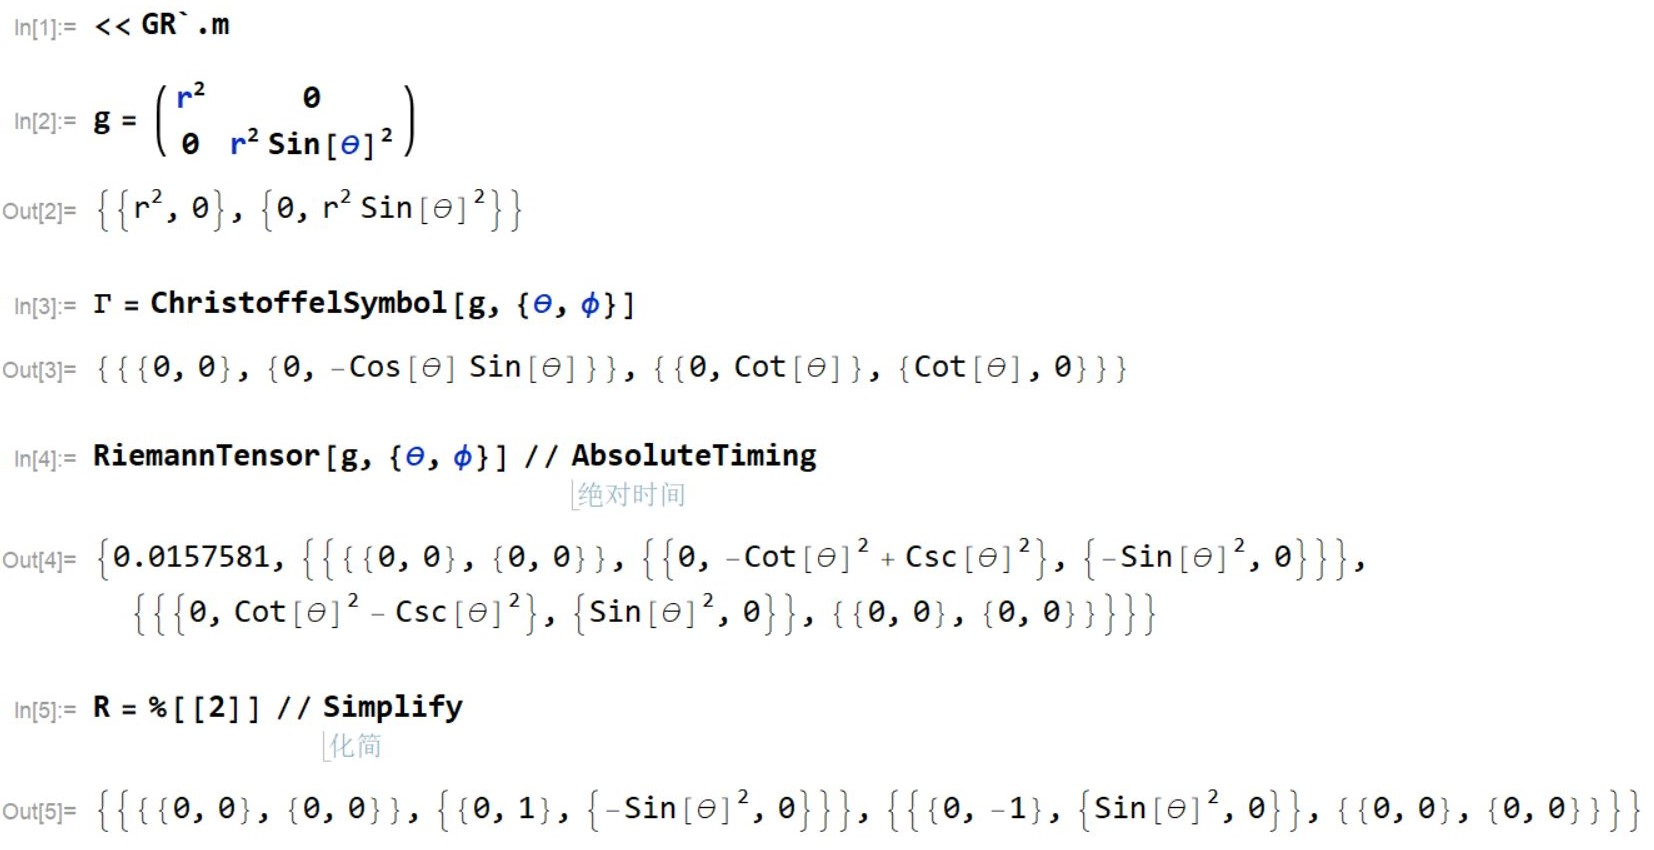
\includegraphics[width=0.8\textwidth]{pictures/1}
			\caption{将第13题扔给麦酱计算}\label{f3.1}
		\end{figure}
	\end{jie}

	\item \hypertarget{3.14}{}求度规$\dd{s}^2 = \Omega^2(t,x) \left(-\dd{t}^2 + \dd{x}^2\right) $的黎曼张量在$\{t,x\}$系的全部分量(在结果中以$\dot{\Omega} $和$ \Omega^\prime$ 分别代表函数 $\Omega$对$t$和$x$的偏导数)。

	\begin{jie}
		先求克氏符。
		\begin{align*}
		\ChristoffelSymbol{t}{t}{t} &= \christoffelSymbol{t}{t}{t}{t}\\
		&= \frac{\dot{\Omega}}{\Omega}\\
		\ChristoffelSymbol{t}{t}{x} &= \christoffelSymbol{t}{t}{x}{t}\\
		&= \frac{\Omega^\prime}{\Omega}\\
		\ChristoffelSymbol{t}{x}{x} &= \christoffelSymbol{t}{x}{x}{t}\\
		&= \frac{\dot{\Omega}}{\Omega}\\
		\ChristoffelSymbol{x}{t}{t} &= \christoffelSymbol{x}{t}{t}{x}\\
		&= \frac{\Omega^\prime}{\Omega}\\
		\ChristoffelSymbol{x}{t}{x} &= \christoffelSymbol{x}{t}{x}{x}\\ \displaybreak[1]
		&= \frac{\dot{\Omega}}{\Omega}\\
		\ChristoffelSymbol{x}{x}{x} &= \christoffelSymbol{x}{x}{x}{x}\\
		&= \frac{\Omega^\prime}{\Omega}
		\end{align*}
		则
		\begin{align*}
		\tensor{R}{_t_x_t^t}&= \riemannR{t}{x}{t}{t}{t} + \ChristoffelSymbol{x}{t}{t} \ChristoffelSymbol{t}{x}{x} - \ChristoffelSymbol{x}{t}{x} \ChristoffelSymbol{t}{t}{x}\\
		&= \frac{\Omega \dot{\Omega}^\prime - \dot{\Omega} \Omega^\prime}{\Omega^2} - \frac{\Omega \dot{\Omega}^\prime - \dot{\Omega} \Omega^\prime}{\Omega^2} + \frac{\dot{\Omega}\Omega^\prime}{\Omega^2} - \frac{\dot{\Omega}\Omega^\prime}{\Omega^2} + \frac{\dot{\Omega}\Omega^\prime}{\Omega^2} -\frac{\dot{\Omega}\Omega^\prime}{\Omega^2}\\
		&= 0\\
		\tensor{R}{_t_x_x^t}&=\riemannR{t}{x}{x}{t}{t}+ \ChristoffelSymbol{x}{x}{t} \ChristoffelSymbol{t}{x}{x}- \ChristoffelSymbol{x}{x}{x} \ChristoffelSymbol{t}{t}{x}\\
		&=\frac{\Omega\Omega^{\prime\prime}- {\Omega^{\prime}}^2}{\Omega^2}- \frac{\Omega\ddot{\Omega}- \dot{\Omega}^2}{\Omega^2}+ \frac{{\Omega^\prime}^2}{\Omega^2}- \frac{\dot{\Omega}^2}{\Omega^2}+ \frac{\dot{\Omega}^2}{\Omega^2}- \frac{{\Omega^\prime}^2}{\Omega^2}\\
		&=\frac{\Omega \left( \Omega^{\prime\prime}- \ddot{\Omega} \right)+ \dot{\Omega}^2 - {\Omega^\prime}^2 }{\Omega^2}\\
		\tensor{R}{_t_x_t^x}&= \riemannR{t}{x}{t}{x}{t}+ \ChristoffelSymbol{x}{t}{t} \ChristoffelSymbol{x}{x}{x}- \ChristoffelSymbol{x}{t}{x} \ChristoffelSymbol{x}{t}{x}\\
		&=\frac{\Omega\Omega^{\prime\prime}- {\Omega^\prime}^2}{\Omega^2}- \frac{\Omega\ddot{\Omega}- \dot{\Omega}^2}{\Omega^2} + \frac{\dot{\Omega}^2}{\Omega^2}- \frac{{\Omega^\prime}^2}{\Omega^2}+ \frac{{\Omega^\prime}^2}{\Omega^2}- \frac{\dot{\Omega}^2}{\Omega^2}\\
		&=\frac{\Omega \left( \Omega^{\prime\prime}- \ddot{\Omega} \right)+ \dot{\Omega}^2 - {\Omega^\prime}^2 }{\Omega^2}\\
		\tensor{R}{_t_x_x^x}&= \riemannR{t}{x}{x}{x}{t}+ \ChristoffelSymbol{x}{x}{t} \ChristoffelSymbol{x}{x}{x}- \ChristoffelSymbol{x}{x}{x} \ChristoffelSymbol{x}{t}{x}\\
		&=  \frac{\Omega \dot{\Omega}^\prime - \dot{\Omega} \Omega^\prime}{\Omega^2}-  \frac{\Omega \dot{\Omega}^\prime - \dot{\Omega} \Omega^\prime}{\Omega^2}+ \frac{\Omega^\prime\dot{\Omega}}{\Omega^2}- \frac{\Omega^\prime\dot{\Omega}}{\Omega^2}+ \frac{\Omega^\prime\dot{\Omega}}{\Omega^2}- \frac{\Omega^\prime\dot{\Omega}}{\Omega^2}\\
		&=0
		\end{align*}
		故所有非零分量为$\displaystyle \tensor{R}{_t_x_x^t}= -\tensor{R}{_x_t_x^t}=\tensor{R}{_t_x_t^x}= -\tensor{R}{_x_t_t^x}= \frac{\Omega \left( \Omega^{\prime\prime}- \ddot{\Omega} \right)+ \dot{\Omega}^2 - {\Omega^\prime}^2 }{\Omega^2} $。

		本题用上述Mathematica代码解决如图~\ref{f3.2}:
		\begin{figure}[htb]
			\centering
			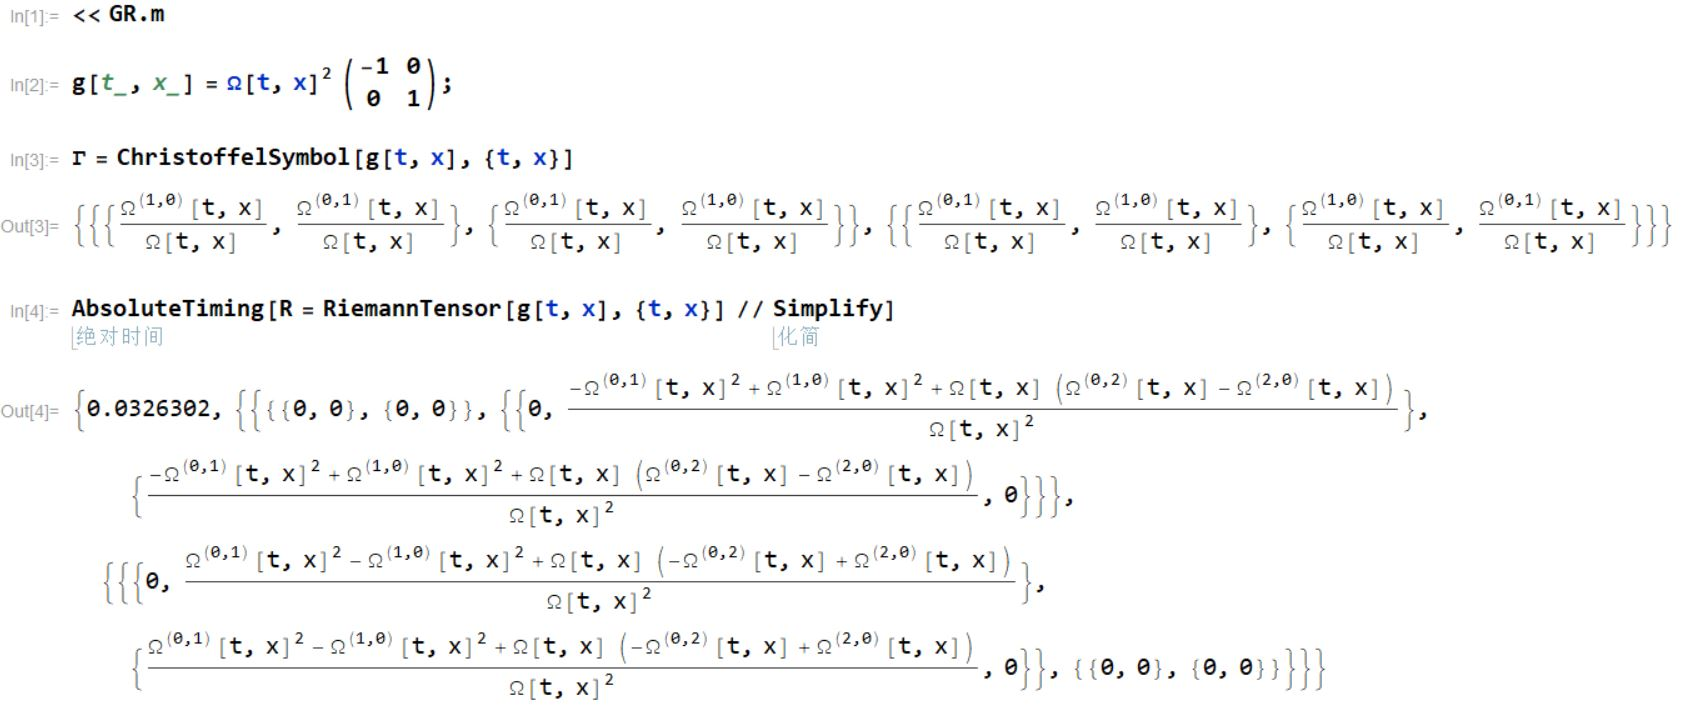
\includegraphics[width=0.8\textwidth]{pictures/2}
			\caption{将第14题扔给麦酱}\label{f3.2}
		\end{figure}
	\end{jie}

	\item \hypertarget{3.15}{}求度规$\dd{s}^2=z^{-1/2} \left(-\dd{t}^2+\dd{z}^2\right)+ z\left(\dd{x}^2+\dd{y}^2\right)$的黎曼张量在$\{t,x,y,z\}$系的全部分量。

	\begin{jie}
		先求克氏符分量。由度规分量的非对角元均为零,克氏符分量\[\ChristoffelSymbol{\sigma}{\mu}{\nu}=\christoffelSymbol{\sigma}{\mu}{\nu}{\sigma}\]。非零分量至少应该满足:$\sigma\mu\nu$至少有两个相等;$\sigma\mu\nu$中至少有一个为$z$(否则导数项全为零)。进一步地,若两个相等,则第三个必为$z$(否则导数项为零);若三个相等,则为$zzz$。即,非零分量满足三个指标中一个为$z$其余两个相同。
		\begin{align*}
		\ChristoffelSymbol{t}{t}{z}&= \christoffelSymbol{t}{t}{z}{t}\\
		&=-\frac{1}{4z}\\
		\ChristoffelSymbol{x}{x}{z}&= \christoffelSymbol{x}{x}{z}{x}\\
		&=\frac{1}{z}\\
		\ChristoffelSymbol{y}{y}{z}&= \christoffelSymbol{y}{y}{z}{y}\\
		&=\frac{1}{z}\\
		\ChristoffelSymbol{z}{t}{t}&= \christoffelSymbol{z}{t}{t}{z}\\
		&=-\frac{1}{4z}\\
		\ChristoffelSymbol{z}{x}{x}&= \christoffelSymbol{z}{x}{x}{z}\\
		&=-\frac{\sqrt{z}}{2}\\
		\ChristoffelSymbol{z}{y}{y}&= \christoffelSymbol{z}{y}{y}{z}\\
		&=-\frac{\sqrt{z}}{2}\\
		\ChristoffelSymbol{z}{z}{z}&= \christoffelSymbol{z}{z}{z}{z}\\
		&=-\frac{1}{4z}
		\end{align*}
		于是所有非零克氏符分量为$\displaystyle \ChristoffelSymbol{t}{t}{z}= \ChristoffelSymbol{t}{z}{t}= -\frac{1}{4z}$,$\displaystyle \ChristoffelSymbol{x}{x}{z}= \ChristoffelSymbol{x}{z}{x} = \ChristoffelSymbol{y}{y}{z}= \ChristoffelSymbol{y}{z}{y}= \frac{1}{z} $,$\displaystyle \ChristoffelSymbol{z}{t}{t}= -\frac{1}{4z}$, $\displaystyle \ChristoffelSymbol{z}{x}{x}= \ChristoffelSymbol{z}{y}{y}= -\frac{\sqrt{z}}{2} $, $\displaystyle \ChristoffelSymbol{z}{z}{z}= -\frac{1}{4z} $。

		由黎曼曲率张量分量表达式$\displaystyle \tensor{R}{_\mu_\nu_\sigma^\rho}= \ChristoffelSymbol{\rho}{\sigma}{{\mu,\nu}}- \ChristoffelSymbol{\rho}{\nu}{{\sigma,\mu}}+ \ChristoffelSymbol{\lambda}{\sigma}{\mu} \ChristoffelSymbol{\rho}{\nu}{\lambda}- \ChristoffelSymbol{\lambda}{\nu}{\sigma} \ChristoffelSymbol{\rho}{\mu}{\lambda} $,注意到上述克氏符非零项的规律,黎曼张量的非零分量至少应该满足 $\mu \neq \nu$并且:
		\begin{enumerate}
			\item $\rho$不为$z$时,导数项非零的条件是$\mu\nu$中有一个为$z$另一个和$\rho$相同且$\sigma=z$;下面分类讨论后两项。
			\begin{enumerate}
				\item $\mu\nu$中有一个为$z$时,设$\nu=z$,$\displaystyle \tensor{R}{_\mu_z_\sigma^\rho}= \ChristoffelSymbol{\rho}{\sigma}{{\mu,z}}- \cancel{\ChristoffelSymbol{\rho}{z}{{\sigma,\mu}}}+ \ChristoffelSymbol{\lambda}{\sigma}{\mu} \ChristoffelSymbol{\rho}{z}{\lambda}- \ChristoffelSymbol{\lambda}{z}{\sigma} \ChristoffelSymbol{\rho}{\mu}{\lambda} $,倒数第二项中$\rho z\lambda$的组合为满足克氏符非零项“一个为$z$其余两个相同”的特征,要求$\lambda=\rho$;最后一项中$\lambda z\sigma $的组合要求$\lambda=\sigma$,于是$\displaystyle \tensor{R}{_\mu_z_\sigma^\rho}= \ChristoffelSymbol{\rho}{\sigma}{{\mu,z}}+ \ChristoffelSymbol{\rho}{\sigma}{\mu} \ChristoffelSymbol{\rho}{z}{\rho}- \ChristoffelSymbol{\sigma}{z}{\sigma} \ChristoffelSymbol{\rho}{\mu}{\sigma} $,第一项非零要求$\mu=\rho$且$\sigma=z$,第二项非零要求$\mu=\rho $且$\sigma=z$;最后一项非零要求$\mu=\rho$且$\sigma=z$,于是非零项为$\displaystyle \tensor{R}{_\rho_z_z^\rho}= \ChristoffelSymbol{\rho}{z}{{\rho,z}}+ \ChristoffelSymbol{\rho}{z}{\rho} \ChristoffelSymbol{\rho}{z}{\rho}- \ChristoffelSymbol{z}{z}{z} \ChristoffelSymbol{\rho}{\rho}{z} $。
				\item $\mu\nu$均不为$z$时,求导项为零,$\displaystyle \tensor{R}{_\mu_\nu_\sigma^\rho}=  \ChristoffelSymbol{\lambda}{\sigma}{\mu} \ChristoffelSymbol{\rho}{\nu}{\lambda}- \ChristoffelSymbol{\lambda}{\nu}{\sigma} \ChristoffelSymbol{\rho}{\mu}{\lambda} $,第一项中$\rho\nu\lambda$的组合要求$\lambda=z $且$\nu=\rho $,第二项中$\rho\mu\lambda$的组合要求$\lambda=z$且$\mu=\rho$,于是$\displaystyle \tensor{R}{_\mu_\nu_\sigma^\rho}=  \ChristoffelSymbol{z}{\sigma}{\mu} \ChristoffelSymbol{\rho}{\nu}{z}- \ChristoffelSymbol{z}{\nu}{\sigma} \ChristoffelSymbol{\rho}{\mu}{z} $,$\mu\nu$中至少一个与$\rho$相同。不妨设$\mu=\rho$,则$\displaystyle \tensor{R}{_\rho_\nu_\sigma^\rho}=- \ChristoffelSymbol{z}{\nu}{\sigma} \ChristoffelSymbol{\rho}{\rho}{z} $,非零项为$\displaystyle \tensor{R}{_\rho_\nu_\nu^\rho}=- \ChristoffelSymbol{z}{\nu}{\nu} \ChristoffelSymbol{\rho}{\rho}{z} $。
			\end{enumerate}
			\item $\rho$为$z$时,则后两项中$\lambda$应分别取$\nu$和$\mu$,即$\displaystyle \tensor{R}{_\mu_\nu_\sigma^z}= \ChristoffelSymbol{z}{\sigma}{{\mu,\nu}}- \ChristoffelSymbol{z}{\nu}{{\sigma,\mu}}+ \ChristoffelSymbol{\nu}{\sigma}{\mu} \ChristoffelSymbol{z}{\nu}{\nu}- \ChristoffelSymbol{\mu}{\nu}{\sigma} \ChristoffelSymbol{z}{\mu}{\mu} $,若$\mu\nu$均不为$z$,则导数项为零,而后两项中$\ChristoffelSymbol{\nu}{\sigma}{\mu}$和$ \ChristoffelSymbol{\mu}{\nu}{\sigma} $无论$\sigma$如何取都不能满足克氏符非零项“一个为$z$其余两个相同”的特征,故$\mu \nu$中有一个为$z$,考虑到指标$\mu \nu$反称只需计算偶排列,于是我们有$\nu=z$,非零项为$\displaystyle \tensor{R}{_\mu_z_\sigma^z}= \ChristoffelSymbol{z}{\sigma}{{\mu,z}}+ \ChristoffelSymbol{z}{\sigma}{\mu} \ChristoffelSymbol{z}{z}{z}- \ChristoffelSymbol{\mu}{z}{\sigma} \ChristoffelSymbol{z}{\mu}{\mu} $,又看出必须有$\mu= \sigma$,于是非零项为$\displaystyle \tensor{R}{_\mu_z_\mu^z}= \ChristoffelSymbol{z}{\mu}{{\mu,z}}+ \ChristoffelSymbol{z}{\mu}{\mu} \ChristoffelSymbol{z}{z}{z}- \ChristoffelSymbol{\mu}{z}{\mu} \ChristoffelSymbol{z}{\mu}{\mu} $。
		\end{enumerate}
	综上,可能非零项为
	\begin{align*}
	\tensor{R}{_\rho_z_z^\rho}&= \ChristoffelSymbol{\rho}{z}{{\rho,z}}+ \ChristoffelSymbol{\rho}{z}{\rho} \ChristoffelSymbol{\rho}{z}{\rho}- \ChristoffelSymbol{z}{z}{z} \ChristoffelSymbol{\rho}{\rho}{z}, & \rho&=t,x,y\\
	\tensor{R}{_\rho_\nu_\nu^\rho}&=- \ChristoffelSymbol{z}{\nu}{\nu} \ChristoffelSymbol{\rho}{\rho}{z}, & \rho,\nu&=t,x,y \\
	\tensor{R}{_\mu_z_\mu^z}&= \ChristoffelSymbol{z}{\mu}{{\mu,z}}+ \ChristoffelSymbol{z}{\mu}{\mu} \ChristoffelSymbol{z}{z}{z}- \ChristoffelSymbol{\mu}{z}{\mu} \ChristoffelSymbol{z}{\mu}{\mu}, & \mu&=t,x,y.
	\end{align*}
	又注意到$x$与$y$的对称性,只需计算$x$而不用计算$y$、只需计算$xyyx$不用计算$yxxy$。下面按以上规则计算可能的非零分量。
	\begin{align*}
	\tensor{R}{_t_x_x^t}&=- \ChristoffelSymbol{z}{x}{x} \ChristoffelSymbol{t}{t}{z}\\ \displaybreak[1]
	&=-\frac{1}{8\sqrt{z}}\\
	\tensor{R}{_t_z_z^t}&= \ChristoffelSymbol{t}{z}{{t,z}}+ \ChristoffelSymbol{t}{z}{t} \ChristoffelSymbol{t}{z}{t}- \ChristoffelSymbol{z}{z}{z} \ChristoffelSymbol{t}{t}{z}\\
	&= \frac{1}{4z^2} +\frac{1}{16z^2}-\frac{1}{16z^2} \\ \displaybreak[1]
	&= \frac{1}{4z^2}\\
	\tensor{R}{_x_y_y^x}&=- \ChristoffelSymbol{z}{y}{y} \ChristoffelSymbol{x}{x}{z}\\ \displaybreak[1]
	&=\frac{1}{4\sqrt{z}}\\
	\tensor{R}{_x_z_z^x}&= \ChristoffelSymbol{x}{z}{{x,z}}+ \ChristoffelSymbol{x}{z}{x} \ChristoffelSymbol{x}{z}{x}- \ChristoffelSymbol{z}{z}{z} \ChristoffelSymbol{x}{x}{z}\\
	&=-\frac{1}{2z^2}+ \frac{1}{4z^2}+ \frac{1}{8z^2}\\ \displaybreak[1]
	&=-\frac{1}{8z^2}\\
	\tensor{R}{_t_z_t^z}&= \ChristoffelSymbol{z}{t}{{t,z}}+ \ChristoffelSymbol{z}{t}{t} \ChristoffelSymbol{z}{z}{z}- \ChristoffelSymbol{t}{z}{t} \ChristoffelSymbol{z}{t}{t}\\
	&=\frac{1}{4z^2}+\frac{1}{16z^2}- \frac{1}{16z^2}\\ \displaybreak[1]
	&=\frac{1}{4z^2}\\
	\tensor{R}{_x_z_x^z}&= \ChristoffelSymbol{z}{x}{{x,z}}+ \ChristoffelSymbol{z}{x}{x} \ChristoffelSymbol{z}{z}{z}- \ChristoffelSymbol{x}{z}{x} \ChristoffelSymbol{z}{x}{x}\\
	&=-\frac{1}{4\sqrt{z}}+\frac{1}{8\sqrt{z}}+\frac{1}{4\sqrt{z}}\\
	&=\frac{1}{8\sqrt{z}}
	\end{align*}
	于是所有非零分量为
	\begin{align*}
	\tensor{R}{_t_x_x^t}&=-\tensor{R}{_x_t_x^t}=\tensor{R}{_t_y_y^t}= - \tensor{R}{_y_t_y^t}=-\frac{1}{8\sqrt{z}}\\
	\tensor{R}{_t_z_z^t}&=-\tensor{R}{_z_t_z^t}=\frac{1}{4z^2}\\
	\tensor{R}{_x_y_y^x}&=\tensor{R}{_y_x_x^y}=\frac{1}{4\sqrt{z}}\\
	\tensor{R}{_x_z_z^x}&=-\tensor{R}{_z_x_z^x}= \tensor{R}{_y_z_z^y}=-\tensor{R}{_z_y_z^y}=-\frac{1}{8z^2}\\
	\tensor{R}{_t_z_t^z}&=-\tensor{R}{_z_t_t^z}=\frac{1}{4z^2}\\
	\tensor{R}{_x_z_x^z}&=-\tensor{R}{_z_x_x^z}=\frac{1}{8\sqrt{z}}
	\end{align*}
	PS:我第一遍手算的算了几个小时(论经常抄错指标的悲惨……)所以还是分析一番,分类讨论分量非零条件顺便化简的好……当然最省事的还是交给麦酱,秒出结果……
	\end{jie}

	\item \hypertarget{3.16}{}设$\alpha(z)$,$\beta(z)$,$\gamma(z)$为任意函数,$h=t+ \alpha(z)x+\beta(z)y+\gamma(z) $,求度规\[ \dd{s}^2= -\dd{t}^2 + \dd{x}^2 +\dd{y}^2 +h^2\dd{z}^2 \] 的黎曼张量在$\{t,x,y,z\}$系的全部分量。

	\begin{jie}
		首先求克氏符分量,由于度规分量矩阵的非对角元全为零,\[\displaystyle \ChristoffelSymbol{\sigma}{\mu}{\nu}=\christoffelSymbol{\sigma}{\mu}{\nu}{\sigma}\],导数项非零要求$\sigma\mu\nu$中有两个取$z$。
		\begin{align*}
		\ChristoffelSymbol{t}{z}{z}&=\christoffelSymbol{t}{z}{z}{t}\\ \displaybreak[1]
		&= h\\
		\ChristoffelSymbol{x}{z}{z}&=\christoffelSymbol{x}{z}{z}{x}\\ \displaybreak[1]
		&=-h\alpha\\
		\ChristoffelSymbol{y}{z}{z}&=\christoffelSymbol{y}{z}{z}{y}\\ \displaybreak[1]
		&=-h\beta\\
		\ChristoffelSymbol{z}{z}{t}&=\christoffelSymbol{z}{z}{t}{z}\\ \displaybreak[1]
		&=\frac{1}{h}\\
		\ChristoffelSymbol{z}{z}{x}&=\christoffelSymbol{z}{z}{x}{z}\\ \displaybreak[1]
		&=\frac{\alpha}{h}\\
		\ChristoffelSymbol{z}{z}{y}&= \christoffelSymbol{z}{z}{y}{z}\\ \displaybreak[1]
		&=\frac{\beta}{h}\\
		\ChristoffelSymbol{z}{z}{z}&=\christoffelSymbol{z}{z}{z}{z}\\
		&=\frac{x\alpha^\prime+y\beta^\prime+\gamma^\prime}{h}
		\end{align*}
		黎曼张量分量表达式为$\displaystyle \tensor{R}{_\mu_\nu_\sigma^\rho}= \ChristoffelSymbol{\rho}{\sigma}{{\mu,\nu}}- \ChristoffelSymbol{\rho}{\nu}{{\sigma,\mu}}+ \ChristoffelSymbol{\lambda}{\sigma}{\mu} \ChristoffelSymbol{\rho}{\nu}{\lambda}- \ChristoffelSymbol{\lambda}{\nu}{\sigma} \ChristoffelSymbol{\rho}{\mu}{\lambda} $,下面讨论分量非零条件。
		\begin{enumerate}
			\item $\rho$不取$z$。后两项求和中$\lambda=z$,且$\mu\nu$必有一取$z$。由于前两个指标反称,设$\nu$取$z$,则$\displaystyle \tensor{R}{_\mu_z_\sigma^\rho}= \cancel{\ChristoffelSymbol{\rho}{\sigma}{{\mu,z}}}- \ChristoffelSymbol{\rho}{z}{{\sigma,\mu}}+ \ChristoffelSymbol{z}{\sigma}{\mu} \ChristoffelSymbol{\rho}{z}{z}- \ChristoffelSymbol{z}{z}{\sigma} \cancel{\ChristoffelSymbol{\rho}{\mu}{z}} $,又可看出$\sigma=z$,于是非零分量为$\displaystyle \tensor{R}{_\mu_z_z^\rho}=- \ChristoffelSymbol{\rho}{z}{{z,\mu}}+ \ChristoffelSymbol{z}{z}{\mu} \ChristoffelSymbol{\rho}{z}{z} $。
			\item $\rho$取$z$。
			\begin{enumerate}
				\item $\nu$取$z$。则$\displaystyle \tensor{R}{_\mu_z_\sigma^z}= \ChristoffelSymbol{z}{\sigma}{{\mu,z}}- \ChristoffelSymbol{z}{z}{{\sigma,\mu}}+ \ChristoffelSymbol{\lambda}{\sigma}{\mu} \ChristoffelSymbol{z}{z}{\lambda}- \ChristoffelSymbol{\lambda}{z}{\sigma} \ChristoffelSymbol{z}{\mu}{\lambda} $,倒数第二项中$\lambda\sigma\mu $的组合要求$\lambda=z$,最后一项中$z\mu\lambda$的组合要求$\lambda=z$。
				\begin{enumerate}
					\item $\sigma=z$,则$\displaystyle \tensor{R}{_\mu_z_z^z}= \ChristoffelSymbol{z}{z}{{\mu,z}}- \ChristoffelSymbol{z}{z}{{z,\mu}}+\cancel{\ChristoffelSymbol{z}{z}{\mu} \ChristoffelSymbol{z}{z}{z}- \ChristoffelSymbol{z}{z}{z} \ChristoffelSymbol{z}{\mu}{z}}  $;
					\item $\sigma\neq z$,则$\displaystyle \tensor{R}{_\mu_z_\sigma^z}= \cancel{\ChristoffelSymbol{z}{\sigma}{{\mu,z}}}- \ChristoffelSymbol{z}{z}{{\sigma,\mu}}+ \cancel{\ChristoffelSymbol{z}{\sigma}{\mu}} \ChristoffelSymbol{z}{z}{z}- \ChristoffelSymbol{z}{z}{\sigma} \ChristoffelSymbol{z}{\mu}{z} $。
				\end{enumerate}
			\item $\mu\nu$均不取$z$。则$\displaystyle \tensor{R}{_\mu_\nu_\sigma^z}= \ChristoffelSymbol{z}{\sigma}{{\mu,\nu}}- \ChristoffelSymbol{z}{\nu}{{\sigma,\mu}}+ \ChristoffelSymbol{\lambda}{\sigma}{\mu} \ChristoffelSymbol{z}{\nu}{\lambda}- \ChristoffelSymbol{\lambda}{\nu}{\sigma} \ChristoffelSymbol{z}{\mu}{\lambda} $,后两项中$\lambda$均取$z$,且$\sigma=z$。则$\displaystyle \tensor{R}{_\mu_\nu_z^z}= \ChristoffelSymbol{z}{z}{{\mu,\nu}}- \ChristoffelSymbol{z}{\nu}{{z,\mu}}+ \cancel{\ChristoffelSymbol{z}{z}{\mu} \ChristoffelSymbol{z}{\nu}{z}- \ChristoffelSymbol{z}{\nu}{z} \ChristoffelSymbol{z}{\mu}{z}} $。
			\end{enumerate}
		\end{enumerate}
	综上,仅考虑哪些克氏符非零,可以将可能的非零分量确定到如下四种情况:
	\begin{align*}
	\tensor{R}{_\mu_z_z^\rho}&=- \ChristoffelSymbol{\rho}{z}{{z,\mu}}+ \ChristoffelSymbol{z}{z}{\mu} \ChristoffelSymbol{\rho}{z}{z}, & \mu,\rho&=t,x,y \\
	\tensor{R}{_\mu_z_z^z}&= \ChristoffelSymbol{z}{z}{{\mu,z}}- \ChristoffelSymbol{z}{z}{{z,\mu}}, & \mu&=t,x,y \\
	\tensor{R}{_\mu_z_\sigma^z}&=- \ChristoffelSymbol{z}{z}{{\sigma,\mu}}- \ChristoffelSymbol{z}{z}{\sigma} \ChristoffelSymbol{z}{\mu}{z}, & \mu,\sigma&=t,x,y \\
	\tensor{R}{_\mu_\nu_z^z}&= \ChristoffelSymbol{z}{z}{{\mu,\nu}}- \ChristoffelSymbol{z}{\nu}{{z,\mu}}, & \mu,\nu&=t,x,y
	\end{align*}
	但是进一步考虑那些非零的克氏符分量的具体形式,由于\[\ChristoffelSymbol{z}{z}{\mu}= \frac{\pdv{h}{x^\mu}}{h},\]于是\[ \ChristoffelSymbol{z}{z}{{\mu,\nu}}=- \frac{\pdv{h}{x^\mu}\pdv{h}{x^\nu}}{h^2}= \ChristoffelSymbol{z}{z}{{\nu,\mu}}= \ChristoffelSymbol{z}{z}{\mu} \ChristoffelSymbol{z}{z}{\nu},\]故第二三四种情况均为零,还剩下\[
	\tensor{R}{_\mu_z_z^\rho}=- \ChristoffelSymbol{\rho}{z}{{z,\mu}}+ \ChristoffelSymbol{z}{z}{\mu} \ChristoffelSymbol{\rho}{z}{z}\qc\quad \rho=t,x,y \]
	而\[ \ChristoffelSymbol{\rho}{z}{z}=-\tensor{g}{^\rho^\rho} h \pdv{h}{x^\rho} \]可以观察发现
	\begin{align*}
	\ChristoffelSymbol{\rho}{z}{{z,\mu}}&=-\tensor{g}{^\rho^\rho}\pdv{h}{x^\rho} \pdv{h}{x^\mu}\\
	&=\left(-\tensor{g}{^\rho^\rho} h \pdv{h}{x^\mu}\right) \left(\frac{\pdv{h}{x^\mu}}{h}\right)\\
	&=\ChristoffelSymbol{z}{z}{\mu} \ChristoffelSymbol{\rho}{z}{z}
	\end{align*}
	于是本题的黎曼张量的所有分量全为零。扔给麦酱验证如图~\ref{f3.3}
	\begin{figure}[htb]
		\centering
		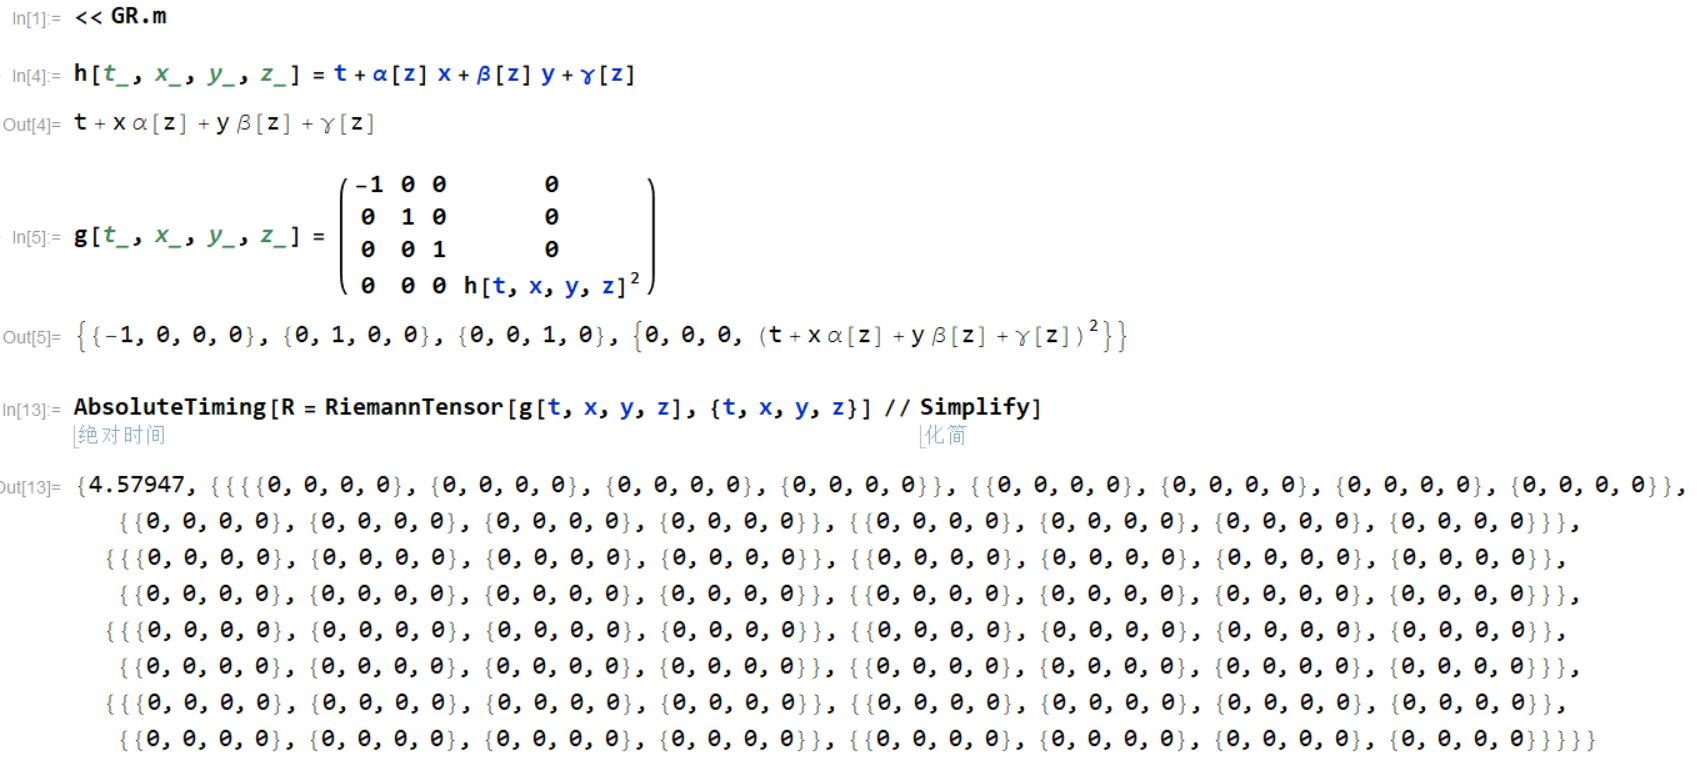
\includegraphics[width=0.8\textwidth]{pictures/3}
		\caption{Mathematica验证第16题}\label{f3.3}
	\end{figure}
	\end{jie}

	\item 试证2维广义黎曼空间的爱因斯坦张量为零。提示:2维广义黎曼空间的黎曼张量只有一个独立分量。

	\begin{zm}
		记$r\equiv\tensor{R}{_1_2_1_2} $,则
		\begin{align*}
		\tensor{R}{_2_1_1_2}&=-r\\
		\tensor{R}{_1_2_2_1}&=-r\\
		\tensor{R}{_2_1_2_1}&=r
		\end{align*}
		于是里奇张量$\tensor{R}{_a_c}:=\tensor{g}{^b^d} \tensor{R}{_a_b_c_d}$的分量为
		\begin{align*}
		\tensor{R}{_1_1}&=\tensor{g}{^2^2} \tensor{R}{_1_2^1_2}\\ \displaybreak[1]
		&=r\tensor{g}{^2^2}\\
		\tensor{R}{_1_2}&=\tensor{g}{^2^1} \tensor{R}{_1_2_2_1}\\ \displaybreak[1]
		&=-r\tensor{g}{^2^1}\\
		\tensor{R}{_2_2}&=\tensor{g}{^1^1} \tensor{R}{_2_1_2_1}\\
		&=r\tensor{g}{^1^1},
		\end{align*}
		标量曲率
		\begin{align*}
		R&=\tensor{g}{^a^c} \tensor{R}{_a_c}\\
		&=2r\tensor{g}{^1^1} \tensor{g}{^2^2} -2r \tensor{g}{^1^2} \tensor{g}{^2^1} \\
		&=2rg.
		\end{align*}
		其中$g=\det [g]$为度规分量矩阵的行列式。注意到,里奇张量分量排成的矩阵为
		\begin{align*}
		\left[R\right]&=\left(
		\begin{array}{cc}
		r\tensor{g}{^2^2}&-r\tensor{g}{^2^1}\\
		-r\tensor{g}{^1^2}&r\tensor{g}{^1^1}
		\end{array}
		\right)\\
		&=r\left([g]^{-1}\right)^*\\
		&=rg[g],
		\end{align*}
		其中$A^*$代表$A$的伴随矩阵。于是爱因斯坦张量$ \displaystyle \tensor{G}{_a_b}=\tensor{R}{_a_b}-\frac{1}{2} R \tensor{g}{_a_b}$的分量矩阵为
		\begin{align*}
		[G]&=[R]-\frac{1}{2} R [g]\\
		&=rg[g]-rg[g]\\
		&=0.
		\end{align*}
	\end{zm}

\end{xiti}

	% !TeX root = ../document.tex

\chapter{李导数、Killing场和超曲面}
\begin{xiti}
	\item 试证由式(4-1-1)定义的$\tensor{\left(\phi_* v\right)}{^a}$满足\S 2.2定义2对矢量的两个要求,从而的确是$\phi(p)$点的矢量。
	
	\begin{zm}
		\begin{enumerate}
			\item $\left(\phi_* v\right) (f+g)= v(\phi^*(f+g))=v(\phi^* f)+ v(\phi^* g)= \left(\phi_* v\right)(f)+ \left(\phi_* v\right)(g) $;
			\item $\left(\phi_* v\right)(fg)= v(\phi^*(fg))= v(\phi^*(f)\phi^*(g))= \left.\phi^*(f)\right|_p v(\phi^* g)+ \left.\phi^*(g)\right|_p v(\phi^* f)= \left. f \right|_{\phi(p)}\left(\phi_* v\right)(g)+ \left. g \right|_{\phi(p)}\left(\phi_* v\right)(f) $。
		\end{enumerate}
	\end{zm}
	
	\item 试证定理4-1-1、4-1-2和4-1-3.
	
	\begin{zm}
		\begin{enumerate}
			\item[(1)] 定理4-1-1如下:
			\begin{yl}{Thm}
				\hypertarget{thm4.1.1}{}$\phi_* \colon V_p \rightarrow V_{\phi(p)} $是线性映射,即\[ \phi_* (\alpha \tensor{u}{^a} + \beta \tensor{v}{^a})= \alpha \phi_* \tensor{u}{^a} + \beta \phi_* \tensor{v}{^a} ,\quad \forall \tensor{u}{^a},\tensor{v}{^a}\in V_p\qc \alpha, \beta \in \mathbb{R}. \]
			\end{yl}
		    \begin{yl}{Prf}
			    $\forall f\in \F_N $,
			    \begin{align*}
			    \left[\phi_*(\alpha u+\beta v)\right](f)&=(\alpha u+\beta v)(\phi^* f)\\
			    &=\alpha u(\phi^* f)+ \beta v (\phi^* f)\\
			    &=\alpha \left(\phi_* u\right)(f)+ \beta \left(\phi_* v\right) (f)\\
			    &=\left(\alpha \phi_* u+ \beta \phi_* v \right)(f)
			    \end{align*}
		    \end{yl}
	        \item[(2)] 定理4-1-2如下:
	        \begin{yl}{Thm}
	        	设$C(t)$是$M$中的曲线,$\tensor{T}{^a}$为曲线在$C(t_0)$的切矢,则$\phi_* \tensor{T}{^a}\in V_{\phi(C(t_0))}$是曲线$\phi(C(t))$在$\phi(C(t_0))$点的切矢(曲线切矢的像是曲线像的切矢)。
	        \end{yl}
            \begin{yl}{Prf}
            	$\forall f\in \F_N$,
            	\begin{align*}
            	\displaybreak[1] \left(\phi_* T\right)(f)&= T (\phi^* f)\\\displaybreak[1]
            	&=\left. \dv{t}(\left(\phi^* f\right)\circ C(t)) \right|_{t_0}\\
            	&=\left. \dv{t}(f\circ \phi \circ C(t)) \right|_{t_0}\\
            	&=T^\prime(f),
            	\end{align*}
            	其中$\tensor{{T^\prime}}{^a}$是曲线$\phi(C(t))$在$\phi(C(t_0))$的切矢。于是$\tensor{T}{^a}= \tensor{{T^\prime}}{^a}$。
            \end{yl}
            \item[(3)] 定理4-1-3如下:
            \begin{yl}{Thm}
            	$\left. \tensor{\left(\phi_*T\right) }{^{\mu_1 \cdots \mu_k}_{\nu_1 \cdots \nu_l }}\right|_{\phi(p)}= \left. \tensor{{T^\prime}}{^{\mu_1 \cdots \mu_k}_{\nu_1 \cdots \nu_l}} \right|_p\qc \forall T\in \F_M(k,l), $\\式中左边是新点$\phi(p)$的新张量$\phi_* T$在老坐标系$\{y^\mu\}$的分量,右边是老点$p$的老张量$T$在新坐标系$\{{x^\prime}^\mu \}$的分量。
            \end{yl}
            \begin{yl}{Prf}
            	由定理4-1-2,坐标基矢作为坐标线的切矢,满足\[ \phi_* \left[ \left. \tensor{\left(\pdv{{x^\prime}^\mu}\right)}{^a} \right|_p \right]=\left. \tensor{\left(\pdv{y^\mu}\right)}{^a} \right|_{\phi(p)}, \]于是$\forall \tensor{v}{^a}\in V_{\phi(p)}$,
            	\begin{align*}
            	\phi_* \left[ \left. \tensor{\left(\dd{{x^\prime}^\mu}\right)}{_a} \right|_p \right]\tensor{v}{^a}&= \left. \tensor{ \left( \dd{{x^\prime}^\mu}\right)}{_a} \right|_{p} \tensor{\left(\phi^* v\right)}{^a}\\
            	&=\left(\phi^* v\right) ({x^\prime}^\mu)\\
            	&=v(\phi_* {x^\prime}^\mu)\\
            	&=v(y^\mu)\\
            	&=\left.\tensor{\left(\dd{y^\mu}\right)}{_a} \right|_{\phi(p)} \tensor{v}{^a} 
            	\end{align*}
            	故\[ \phi_* \left[ \left. \tensor{\left(\dd{{x^\prime}^\mu}\right)}{_a} \right|_p \right]=\left.\tensor{\left(\dd{y^\mu}\right)}{_a} \right|_{\phi(p)}, \]于是对任意张量场$T\in\F_M(k,l) $,
            	\begin{align*}
            	&\left. \tensor{\left(\phi_*T\right) }{^{\mu_1 \cdots \mu_k}_{\nu_1 \cdots \nu_l }}\right|_{\phi(p)}\\
            	=&\mspace{2mu}\left. \tensor{\left(\phi_*T\right) }{^{a_1 \cdots a_k}_{b_1 \cdots b_l }}\right|_{\phi(p)} \left. \tensor{ \left( \dd{y^{\mu_1}} \right)}{_{a_1}} \right|_{\phi(p)} \cdots \left. \tensor{ \left( \dd{y^{\mu_k}} \right)}{_{a_k}} \right|_{\phi(p)} \left. \tensor{ \left( \pdv{y^{\nu_1}} \right)}{^{b_1}} \right|_{\phi(p)} \cdots \left. \tensor{ \left( \pdv{y^{\nu_l}} \right)}{^{b_l}} \right|_{\phi(p)}\\ \displaybreak[1]
            	=&\; \left. \tensor{T}{^{a_1 \cdots a_k}_{b_1 \cdots b_l}} \right|_p \left. \tensor{ \left( \dd{{x^\prime}^{\mu_1}} \right)}{_{a_1}} \right|_p \cdots \left. \tensor{ \left( \dd{{x^\prime}^{\mu_k}} \right)}{_{a_k}} \right|_p \left. \tensor{ \left( \pdv{{x^\prime}^{\nu_1}} \right)}{^{b_1}} \right|_p \cdots \left. \tensor{ \left( \pdv{{x^\prime}^{\nu_l}} \right)}{^{b_l}} \right|_p \\ \displaybreak[1]
            	=&\; \left. \tensor{{T^\prime}}{^{\mu_1 \cdots \mu_k}_{\nu_1 \cdots \nu_l}} \right|_p.
            	\end{align*}
            \end{yl}
		\end{enumerate}
	\end{zm}
	
	\item 设$\phi\colon M\rightarrow N$ 为光滑映射,$p \in M $,$\{ y^\mu \}$是$\phi(p)$点某邻域上的坐标,试证
	\begin{displaymath}
	\tensor{\left(\phi_* v\right)}{^a}= v \left( \phi^* y^\mu \right) \tensor{\left(\pd{y^\mu}\right)}{^a}\qc \forall \tensor{v}{^a} \in V_p.
	\end{displaymath}
	
	\begin{zm}
		\begin{align*}
		\tensor{\left(\phi_* v\right)}{^a}&= \left(\phi_* v\right) (y^\mu) \tensor{\left(\pdv{y^\mu}\right)}{^a}\\
		&=v \left(\phi^* y^\mu\right) \tensor{\left(\pdv{y^\mu}\right)}{^a}
		\end{align*}
	\end{zm}
	
	\item 设$M$,$N$是流形,$\phi\colon M\rightarrow N$是微分同胚,$p\in M$,$q\equiv \phi(p)$,试证推前映射$\phi_* \colon V_p \rightarrow V_q $是同构映射。
	
	\begin{zm}
	由定理~\hyperlink{thm4.1.1}{4-1-1}~知$\phi_*$为线性映射,又知其有逆映射$\phi^*$,故为线性同构。
	\end{zm}
	
	\item 设$M$,$N$,$Q$是流形,$\phi\colon M \rightarrow N $和$\psi \colon N \rightarrow Q $是光滑映射。
	\begin{enumerate}
		\item[(a)] 试证$\left( \psi \circ \phi \right)^* f= \left(\phi^* \circ \psi^* \right) f $,$\forall f\in \F_Q $。
		\item[(b)] 试证$\left(\psi \circ \phi \right)_* \tensor{v}{^a}= \psi_*\left( \phi_* \tensor{v}{^a} \right) \qc \forall p\in M,\tensor{v}{^a}\in V_p $。
		\item[(c)] \hypertarget{4.5.c}{}把$\left( \psi \circ \phi \right)^* $和$\phi^* \circ \psi^* $都看作由$\F_Q(0,l) $到$\F_M(0,l) $的映射,试证\[ \left( \psi \circ \phi \right)^*= \phi^* \circ \psi^*. \]
	\end{enumerate}
	
	\begin{zm}
		\begin{enumerate}
			\item[(a)] 按照拉回映射的定义,
			\begin{displaymath}
			\left( \psi \circ \phi \right)^* f= f \circ \psi \circ \phi = \left( \phi^* \circ \psi^*\right) f.
			\end{displaymath}
			\item[(b)] 按照推前映射的定义,$\forall f\in \F_M $,
			\begin{align*}
			\left[\left(\psi\circ\phi\right)_* v \right] (f) &= v \left[ \left( \psi \circ \phi \right)^* f \right]\\
			&= v \left[\phi^*\left( \psi^* f \right) \right]\\
			&= \left( \phi^* v \right) \left( \psi^* f \right)\\
			&= \left[ \psi^* \left(\phi^* v\right) \right] (f).
			\end{align*}
			\item[(c)] $\forall p\in M, v_1,\cdots,v_l \in V_p ,T\in \F_Q(0,l)$,
			\begin{align*}
			&\left. \tensor{\left[\left(\psi\circ\phi\right)^* T\right]  }{_{a_1\cdots a_l}} \right|_p \tensor{\left(v_1\right)}{^{a_1}} \cdots \tensor{\left(v_l\right)}{^{a_l}}\\
			=&\; \left. \tensor{T}{_{a_1 \cdots a_l}} \right|_{\psi(\phi(p))} \left[\left(\psi\circ\phi \right)_* \tensor{\left(v_1\right)}{^{a_1}}\right] \cdots \left[\left(\psi\circ\phi \right)_* \tensor{\left(v_l\right)}{^{a_l}}\right]\\
			=&\; \left. \tensor{T}{_{a_1 \cdots a_l}} \right|_{\psi(\phi(p))} \psi_* \left[\phi_* \tensor{\left(v_1\right)}{^{a_1}}\right] \cdots \psi_* \left[\phi_* \tensor{\left(v_l\right)}{^{a_l}}\right]\\
			=&\tmu \left. \tensor{\left( \psi^* T \right)}{_{a_1\cdots a_l}} \right|_{\phi(p)} \tensor{\left( \phi_* v_1 \right)}{^{a_1}} \cdots \tensor{\left( \phi_* v_l \right)}{^{a_l}}\\
			=&\tmu \left. \tensor{\left[\left( \phi^* \circ \psi^* \right) T\right]  }{_{a_1\cdots a_l}} \right|_p \tensor{\left(v_1\right)}{^{a_1}} \cdots \tensor{\left(v_l\right)}{^{a_l}}
			\end{align*}
		\end{enumerate}
	\end{zm}
	
	\item 设$\phi\colon M \rightarrow N $是微分同胚,$\tensor{v}{^a}$,$\tensor{u}{^a}$是$M$上的矢量场,试证$\phi_*\left( \tensor{\left[ v,u \right]}{^a} \right)= \tensor{\left[\phi_* v,\phi_* u \right]}{^a}$,其中$\tensor{\left[v,u \right]}{^a}$代表对易子。
	
	\begin{zm}
		首先验证一个等式:$\forall v \in \F_M(1,0),f\in \F_N $,有$v(\phi^* f)=\phi^*\left[ (\phi_* v)f \right] $(即把逐点定义的切矢的推前映射表述成场的形式)。$\forall p \in M $,
		\begin{align*}
		\left. \phi^*\left[ (\phi_* v)f \right] \right|_p &= \left. (\phi_* v)f \right|_{\phi(p)} \\
		&= \left. (\phi_* v) \right|_{\phi(p)}(f)\\
		&= \left. v \right|_p \left( \phi^* f \right)\\
		&= \left. v \left( \phi^* f \right) \right|_p.
		\end{align*}
		$\forall f\in \F_N,p\in M $,
		\begin{align*}
		\left. \left(\phi_*\left[v,u\right]\right) \right|_{\phi(p)} (f) &= \left. \left[v,u\right] \right|_p \left(\phi^* f \right)\\
		&= \left. v\right|_p [u(\phi^* f)]- \left. u \right|_p [v(\phi^* f)]\\
		&= \left. v \right|_p \left\{ \phi^* \left[ \left( \phi_* u \right) f \right] \right\} - \left. u \right|_p \left\{ \phi^* \left[ \left( \phi_* v \right) f \right] \right\}\\
		&= \left. \phi_* v \right|_{\phi(p)} \left[ \left( \phi_* u \right) f \right] - \left. \phi_* u \right|_{\phi(p)} \left[ \left( \phi_* v \right) f \right]\\
		&= \left. \left[\phi_* v,\phi_* u\right] \right|_{\phi(p)} (f).
		\end{align*}
	\end{zm}
	
	\item 试证定理4-2-4.
	
	\begin{zm}
		定理4-2-4如下:
		\begin{yl}{Thm}
			\hypertarget{thm4.2.4}{}$\Ld{v} \tensor{\omega}{_a}= \tensor{v}{^b} \Nabla{b} \tensor{\omega}{_a} + \tensor{\omega}{_b} \Nabla{a} \tensor{v}{^b}\qc \forall \tensor{v}{^a} \in \F(1,0),\omega\in \F(0,1), $\\其中$\Nabla{a}$为任意无挠导数算符。
		\end{yl}
	    \begin{yl}{Prf}
	    	由于李导数与缩并可交换顺序,为利用定理4-2-3,向李导数内插入$\tensor{u}{^a}$,计算$\Ld{v}\left(\tensor{\omega}{_a} \tensor{u}{^a} \right) $。$\forall \tensor{u}{^a} \in \F(1,0) $,利用与缩并交换及莱布尼兹律,
	    	\begin{align*}
	    	\Ld{v} \left( \tensor{\omega}{_a} \tensor{u}{^a} \right)&= \tensor{\omega}{_a} \Ld{v} \tensor{u}{^a} + \tensor{u}{^a} \Ld{v} \tensor{\omega}{_a}\\
	    	&=\tensor{\omega}{_a} \tensor{\left[v,u\right]}{^a} + \tensor{u}{^a} \Ld{v} \tensor{\omega}{_a}\\
	    	&= \tensor{\omega}{_a} \left( \tensor{v}{^b} \Nabla{b} \tensor{u}{^a} - \tensor{u}{^b} \Nabla{b} \tensor{v}{^a} \right) + \tensor{u}{^a} \Ld{v} \tensor{\omega}{_a},
	    	\end{align*}
	    	另一方面,根据$\Ld{v}(f)=v(f)$,有
	    	\begin{align*}
	    	\Ld{v} \left( \tensor{\omega}{_a} \tensor{u}{^a} \right) &= \tensor{v}{^b} \Nabla{a} \left( \tensor{\omega}{_b} \tensor{u}{^a} \right)\\
	    	&= \tensor{v}{^b} \tensor{\omega}{_a} \Nabla{b} \tensor{u}{^a} + \tensor{v}{^b} \tensor{u}{^a} \Nabla{b} \tensor{\omega}{_a},
	    	\end{align*}
	    	于是
	    	\begin{gather*}
	    	\displaybreak[1] \cancel{\tensor{\omega}{_a} \tensor{v}{^b} \Nabla{b} \tensor{u}{^a}} - \tensor{\omega}{_a} \tensor{u}{^b} \Nabla{b} \tensor{v}{^a} + \tensor{u}{^a} \Ld{v} \tensor{\omega}{_a}=\cancel{\tensor{v}{^b} \tensor{\omega}{_a} \Nabla{b} \tensor{u}{^a}} + \tensor{v}{^b} \tensor{u}{^a} \Nabla{b} \tensor{\omega}{_a},\\ \displaybreak[1]
	    	\tensor{u}{^a} \Ld{v} \tensor{\omega}{_a} = \tensor{\omega}{_{\cancel{a}b}} \tensor{u}{^{\cancel{b}a}} \Nabla{\cancel{b}a} \tensor{v}{^{\cancel{a}b}} + \tensor{v}{^b} \tensor{u}{^a} \Nabla{b} \tensor{\omega}{_a},\\
	    	\Ld{v} \tensor{\omega}{_a}= \tensor{\omega}{_b} \Nabla{a} \tensor{v}{^b} + \tensor{v}{^b} \Nabla{b} \tensor{\omega}{_a}.
	    	\end{gather*}
	    \end{yl}
	\end{zm}
	
	\item 设$\tensor{v}{^a} \in \F_M(1,0) $,$\tensor{\omega}{_a} \in \F_M(0,1) $,试证对任一坐标系$\{x^\mu \}$有\[ \tensor{\left(\Ld{v} \omega \right)}{_\mu} = \tensor{v}{^\nu} \pdv*{\tensor{\omega}{_\mu}}{x^\nu} + \tensor{\omega}{_\nu} \pdv*{\tensor{v}{^\nu}}{x^\mu}. \]提示:用式(4-2-7)并令其$\Nabla{a}$为$\Partial{a}$。
	
	\begin{zm}
		式(4-2-7)为(也就是定理~\hyperlink{thm4.2.4}{4-2-4}):\[\Ld{v} \tensor{\omega}{_a}= \tensor{v}{^b} \Nabla{b} \tensor{\omega}{_a} + \tensor{\omega}{_b} \Nabla{a} \tensor{v}{^b}\qc \forall \tensor{v}{^a} \in \F(1,0),\omega\in \F(0,1)\]于是
		\begin{align*}
		\tensor{\left( \Ld{v} \omega \right)}{_\mu}&= \tensor{\left(\pdv{x^\mu}\right)}{^a} \Ld{v} \tensor{\omega}{_a}\\
		&= \tensor{\left(\pdv{x^\mu}\right)}{^a} \left( \tensor{v}{^b} \Partial{b} \tensor{\omega}{_a} + \tensor{\omega}{_b} \Partial{a} \tensor{v}{^b} \right)\\
		&= \tensor{v}{^\nu} \pdv{\tensor{\omega}{_\mu}}{x^\nu}+ \tensor{\omega}{_\nu} \pdv{\tensor{v}{^\nu}}{x^\mu}.
		\end{align*}
	\end{zm}

	\item \hypertarget{4.9}{}设$\tensor{u}{^a},\tensor{v}{^a} \in \F_M(1,0) $,则下式作用于任意张量场都成立\[ \left[ \Ld{v},\Ld{u} \right]= \Ld{\left[v,u\right]}\qq{(其中$\left[ \Ld{v},\Ld{u} \right] \equiv \Ld{v}\Ld{u}-\Ld{u}\Ld{v} $).} \]试就作用对象为$f \in \F_M $和$\tensor{w}{^a}\in \F_M(1,0) $的情况给出证明。提示:当作用对象为$\tensor{w}{^a}$时可用雅可比恒等式(第2章习题~\hyperlink{ykb}{8})。
	
	\begin{zm}
		\begin{enumerate}
			\item 作用于标量场:
			\begin{align*}
			\left[\Ld{v},\Ld{u} \right](f)&= \Ld{v}\left(\Ld{u} f \right) - \Ld{u} \left( \Ld{v} f \right)\\
			&=v(u(f))-u(v(f))\\
			&=\left[v,u\right](f)\\
			&= \Ld{\left[v,u\right]}(f).
			\end{align*}
			\item 作用于矢量场:
			\begin{align*}
			\left[ \Ld{v},\Ld{u} \right]w&= \Ld{v} \left( \Ld{u} w \right) - \Ld{u} \left( \Ld{v} w \right)\\
			&=[v,[u,w]]-[u,[v,w]]\\
			&=-\left( \cancel{[u,[w,v]]}+[w,[v,u]] \right)- \cancel{[u,[v,w]]} \\
			&=[[v,u],w]\\
			&=\Ld{[v,u]}w.
			\end{align*}
		\end{enumerate}
	\end{zm}
	
	\item 设$\tensor{F}{_a_b}$是4维闵氏空间上的反称张量场,其在洛伦兹坐标系$\{t,x,y,z \}$的分量为$\tensor{F}{_0_1}=-\tensor{F}{_1_3}=x \rho^{-1} $,$\tensor{F}{_0_2}=-\tensor{F}{_2_3}=y \rho^{-1} $,$\tensor{F}{_0_3}=\tensor{F}{_1_2}=0 $,其中$\rho\equiv \left(x^2+y^2\right)^{1/2} $。试证$\tensor{F}{_a_b}$有旋转对称性,即$\Ld{v} \tensor{F}{_a_b}=0 $,其中$\tensor{v}{^a}=-y \tensor{\left(\pd{x}\right)}{^a}+x \tensor{\left(\pd{y}\right)}{^a} $。
	
	\begin{zm}
		由\[\Ld{v} \tensor{F}{_a_b} = \tensor{v}{^c} \Nabla{c} \tensor{F}{_a_b} + \tensor{F}{_a_c} \Nabla{b} \tensor{v}{^c} + \tensor{F}{_c_b} \Nabla{a} \tensor{v}{^c},\]取$\Nabla{a}$为$\Partial{a}$,有\[  \tensor{\left(\Ld{v} F\right)}{_\mu_\nu} = \tensor{v}{^\sigma} \Partial{\sigma} \tensor{F}{_\mu_\nu} + \tensor{F}{_\mu_\sigma} \Partial{\nu} \tensor{v}{^\sigma} + \tensor{F}{_\sigma_\nu} \Partial{\mu} \tensor{v}{^\sigma}  \]其中第一项求和只对$\sigma=1,2$取,第二三项求和只对$\sigma=1,2$且$\sigma\neq\mu,\nu$取,且$\nu\neq1,2$时第二项不存在,$\mu\neq1,2$时第三项不存在。又易看出$\Ld{v} \tensor{F}{_a_b} $反称,于是
		\begin{align*}
		\tensor{\left(\Ld{v} F\right)}{_0_1} &= \tensor{v}{^1} \Partial{1} \tensor{F}{_0_1} + \tensor{v}{^2} \Partial{2} \tensor{F}{_0_1} + \tensor{F}{_0_2} \Partial{1} \tensor{v}{^2}\\
		&= -y \cdot \frac{y^2}{\rho^3} + x \cdot \left( - \frac{xy}{\rho^3} \right) +\frac{y}{\rho} \cdot (-1) \\
		&=0\\
		\tensor{\left(\Ld{v} F\right)}{_0_2} &= \tensor{v}{^1} \Partial{1} \tensor{F}{_0_2} + \tensor{v}{^2} \Partial{2} \tensor{F}{_0_2} + \tensor{F}{_0_1} \Partial{2} \tensor{v}{^1} \\
		&= -y \cdot \left( - \frac{xy}{\rho^3} \right) + x \cdot \frac{x^2}{\rho^3} + \frac{x}{\rho} \cdot (-1)\\
		&=0\\
		\tensor{\left(\Ld{v} F\right)}{_0_3} &= \tensor{v}{^1} \Partial{1} \tensor{F}{_0_3} + \tensor{v}{^2} \Partial{2} \tensor{F}{_0_3} \\
		&=0\\
		\tensor{\left(\Ld{v} F\right)}{_1_2} &= \tensor{v}{^1} \Partial{1} \tensor{F}{_1_2} + \tensor{v}{^2} \Partial{2} \tensor{F}{_1_2} \\
		&=0\\
		\tensor{\left(\Ld{v} F\right)}{_1_3} &= \tensor{v}{^1} \Partial{1} \tensor{F}{_1_3} + \tensor{v}{^2} \Partial{2} \tensor{F}{_1_3} + \tensor{F}{_2_3} \Partial{1} \tensor{v}{^2} \\
		&=-y \cdot \left( -\frac{y^2}{\rho^3} \right) + x \cdot \frac{xy}{\rho^3} -\frac{y}{\rho} \cdot 1\\
		&=0\\
		\tensor{\left(\Ld{v} F\right)}{_2_3} &= \tensor{v}{^1} \Partial{1} \tensor{F}{_2_3} + \tensor{v}{^2} \Partial{2} \tensor{F}{_2_3} + \tensor{F}{_1_3} \Partial{2} \tensor{v}{^1} \\
		&=-y\cdot \frac{xy}{\rho^3} + x \cdot \left( - \frac{x^2}{\rho^3} \right) - \frac{x}{\rho} \cdot (-1)\\
		&=0.
		\end{align*}
		故$\Ld{v} \tensor{F}{_a_b}=0 $。
	\end{zm}
	
	\item 设$ \tensor{\xi}{^a} $是$\left( M,\tensor{g}{_a_b} \right)$中的 Killing 矢量场,$\Nabla{a}$与$\tensor{g}{_a_b}$相适配,试证$\Nabla{a} \tensor{\xi}{^a}=0 $。
	
	\begin{zm}
		由 Killing 方程,
		\begin{align*}
		\displaybreak[1] \Nabla{a} \tensor{\xi}{^a} &= \tensor{g}{^a^b} \Nabla{a} \tensor{\xi}{_b}\\
		\displaybreak[1] &= \tensor{g}{^a^b} \Nabla{(a} \tensor{\xi}{_{b)}}\\
		&=0.
		\end{align*}
	\end{zm}
	
	\item 设$\tensor{\xi}{^a}$是$\left(M,\tensor{g}{_a_b} \right)$中的 Killing 矢量场,$\phi\colon M\rightarrow M $是等度规映射,试证$\phi_* \tensor{\xi}{^a} $也是$\left( M,\tensor{g}{_a_b} \right) $中的 Killing 矢量场。提示:利用习题~\hyperlink{4.5.c}{5(c)}~中的结论。
	
	\begin{zm}
		记$\tensor{\xi}{^a}$的积分曲线为$C(t)$,它诱导出的单参微分同胚群为$\{\psi_t\}$,则$\phi_* \tensor{\xi}{^a} $的积分曲线是$\phi\circ C(t)$,其诱导出的单参微分同胚群为$\psi^\prime_t=\phi\circ\psi_t \circ \phi^{-1} $。由定义,
		\begin{align*}
		\Ld{\phi_* \xi} \tensor{g}{_a_b} &= \lim\limits_{t\rightarrow 0} \frac{1}{t} \left( {\psi^\prime_t}^* \tensor{g}{_a_b} - \tensor{g}{_a_b} \right)\\
		&= \lim\limits_{t\rightarrow 0} \frac{1}{t}\left[ \left( \phi\circ\psi_t \circ \phi^{-1} \right)^* \tensor{g}{_a_b} - \tensor{g}{_a_b} \right]\\
		&= \lim\limits_{t\rightarrow 0} \frac{1}{t} \left\{\left[ \left(\psi_t\circ\phi^{-1}\right)^* \circ \phi^*\right] \tensor{g}{_a_b} - \tensor{g}{_a_b} \right\}\\
		&= \lim\limits_{t\rightarrow 0} \frac{1}{t}\left[ \left( {\phi^{-1}}^* \circ {\psi_t}^*\right) \tensor{g}{_a_b} - \tensor{g}{_a_b} \right]\\
		&= 0.
		\end{align*}
	\end{zm}

    \item 设$\tensor{\xi}{^a}$,$\tensor{\eta}{^a}$是$\left( M , \tensor{g}{_a_b}\right)$的 Killing 矢量场,试证其对易子$\tensor{\left[ \xi,\eta \right]}{^a}$也是 Killing 矢量场。注:此结论使得$M$上全体 Killing 矢量场的集合不但是矢量空间,而且是李代数(详见中册附录G)。

    \begin{zm}
    	由第~\hyperlink{4.9}{9}~题,知
    	\begin{align*}
    	\Ld{\left[\xi,\eta\right]} \tensor{g}{_a_b} &= \Ld{\xi} \Ld{\eta} \tensor{g}{_a_b} -\Ld{\eta} \Ld{\xi} \tensor{g}{_a_b} \\
    	&=0.
    	\end{align*}
    \end{zm}
	
	\item 设$\tensor{\xi}{^a}$是广义黎曼空间$\left(M, \tensor{g}{_a_b} \right)$的 Killing 矢量场,$\tensor{R}{_a_b_c^d}$是$\tensor{g}{_a_b}$的黎曼曲率张量。
	\begin{enumerate}
		\item[(a)] 试证$\Nabla{a}\Nabla{b}\tensor{\xi}{_c} = - \tensor{R}{_b_c_a^d}\tensor{\xi}{_d} $。注:此式对证明定理4-3-4有重要用处。提示:由$\tensor{R}{_a_b_c^d}$的定义以及 Killing 方程(4-3-1)可知$\Nabla{a} \Nabla{b} \tensor{\xi}{_c} + \Nabla{b} \Nabla{c} \tensor{\xi}{_a} = \tensor{R}{_a_b_c^d} \tensor{\xi}{_d} $。此式称为第一式。作指标替换$a\mapsto b$,$b\mapsto c$,$c\mapsto a$得第二式,再替换一次得第三式。以第一、第二式之和减第三式并利用(3-4-7)便得证。
		\item[(b)] 利用(a)的结果证明$\tensor{\nabla}{^a} \Nabla{a} \tensor{\xi}{_c} = - \tensor{R}{_c_d} \tensor{\xi}{^d} $,其中$\tensor{R}{_c_d}$是里奇张量。
	\end{enumerate}
	
	\begin{zm}
		\begin{enumerate}
			\item[(a)] 由黎曼张量的定义,
			\begin{equation*}
			\left(\Nabla{a}\Nabla{b} - \Nabla{b}\Nabla{a} \right) \tensor{\xi}{_c} = \tensor{R}{_a_b_c^d} \tensor{\xi}{_d}
			\end{equation*}
			由 Killing 方程,$\Nabla{a}\tensor{\xi}{_c} = - \Nabla{c} \tensor{\xi}{_a} $,于是得
			\begin{equation}
			\Nabla{a}\Nabla{b}\tensor{\xi}{_c} + \Nabla{b}\Nabla{c}\tensor{\xi}{_a}= \tensor{R}{_a_b_c^d} \tensor{\xi}{_d}\label{4eq1}
			\end{equation}
			对指标$a,b,c$轮换,得
			\begin{gather}
			\Nabla{b}\Nabla{c}\tensor{\xi}{_a} + \Nabla{c}\Nabla{a}\tensor{\xi}{_b}= \tensor{R}{_b_c_a^d} \tensor{\xi}{_d}\label{4eq2}\\
			\Nabla{c}\Nabla{a}\tensor{\xi}{_b} + \Nabla{a}\Nabla{b}\tensor{\xi}{_c}= \tensor{R}{_c_a_b^d} \tensor{\xi}{_d}\label{4eq3}
			\end{gather}
			$\eqref{4eq1}+\eqref{4eq2}-\eqref{4eq3}$得
			\begin{displaymath}
			2\Nabla{b}\Nabla{c}\tensor{\xi}{_a}=\left( \tensor{R}{_a_b_c^d} + \tensor{R}{_b_c_a^d} - \tensor{R}{_c_a_b^d} \right) \tensor{\xi}{_d}=-2 \tensor{R}{_c_a_b^d} \tensor{\xi}{_d}
			\end{displaymath}
			于是$\Nabla{a}\Nabla{b}\tensor{\xi}{_c} = - \tensor{R}{_b_c_a^d} \tensor{\xi}{_d} $。
			\item[(b)] 由(a),
			\begin{displaymath}
			\tensor{\nabla}{^a}\Nabla{a} \tensor{\xi}{_c} = \tensor{g}{^a^b} \Nabla{b} \Nabla{a} \tensor{\xi}{_c} = -\tensor{g}{^a^b} \tensor{R}{_a_c_b^d} \tensor{\xi}{_d}=- \tensor{R}{_c_d} \tensor{\xi}{^d}.
			\end{displaymath}
		\end{enumerate}
	\end{zm}
	
	\item 验证式(4-3-3)中的$ \tensor{\left(\pd{\eta}\right)}{^a}$的确满足 Killing 方程(4-3-1)。
	
	\begin{zm}
		由$\displaystyle \tensor{\left(\pdv{\eta}\right)}{^a} = x \tensor{\left(\pdv{t}\right)}{^a} + t\tensor{\left(\pdv{x}\right)}{^a} $升指标得
		\begin{displaymath}
		\tensor{\left(\pdv{\eta}\right)}{_a}= \tensor{g}{_a_b} \tensor{\left(\pdv{\eta}\right)}{^b} = - x \tensor{\left(\dd{t}\right)}{_a} + t \tensor{\left(\dd{x}\right)}{_a},
		\end{displaymath}
		于是
		\begin{displaymath}
		\Partial{a}\tensor{\left(\pdv{\eta}\right)}{_b}= - \tensor{\left(\dd{x}\right)}{_a} \tensor{\left(\dd{t}\right)}{_b} + \tensor{\left(\dd{t}\right)}{_a} \tensor{\left(\dd{x}\right)}{_b}=\tensor{\left(\dd{t}\right)}{_{[a}} \tensor{\left(\dd{x}\right)}{_{b]}},
		\end{displaymath}
		这是一个反称张量,故满足$\displaystyle \Nabla{(a} \tensor{\left(\pd{\eta}\right)}{_{b)}}=0 $。
	\end{zm}
	
	\item 找出2维欧氏空间中由$\tensor{R}{^a} = x \tensor{\left(\pd{y}\right)}{^a} - y \tensor{\left(\pd{x}\right)}{^a} $生出的单参等度规群的任一元素$\phi_\alpha$诱导的坐标变换。
	
	\begin{zm}
		积分曲线的参数式满足微分方程
		\begin{displaymath}
		\left\{
		\begin{aligned}
		\dv{x}{t} &= \tensor{R}{^x} = -y,\\
		\dv{y}{t} &= \tensor{R}{^y} = x ,
		\end{aligned}
		\right.
		\end{displaymath}
		并有边界条件
		\begin{displaymath}
		\left\{
		\begin{aligned}
		x(0) &= x_p,\\
		y(0) &= y_p ,
		\end{aligned}
		\right.
		\end{displaymath}
		解得过$p$点的积分曲线的参数式为
		\begin{displaymath}
		\left\{
		\begin{aligned}
		x(t) &= x_p \cos t - y_p \sin t ,\\
		y(t) &= x_p \sin t + y_p \cos t ,
		\end{aligned}
		\right.
		\end{displaymath}
		于是$\phi_\alpha$诱导的坐标变换为
		\begin{displaymath}
		\left\{
		\begin{aligned}
		x^\prime &= x \cos \alpha - y \sin \alpha ,\\
		y^\prime &= x \sin \alpha + y \cos \alpha .
		\end{aligned}
		\right.
		\end{displaymath}
	\end{zm}
	
	\item 设时空$\left(M,\tensor{g}{_a_b}\right)$中的超曲面$\phi[S]$上每点都有类光切矢而无类时切矢(“切矢”指切于$\phi[S]$),试证它必为类光超曲面。提示:\circled{1}证明与类时矢量$\tensor{t}{^a}$正交的矢量必类空[选正交归一基底$\{ \tensor{\left(e_\mu\right)}{^a} \}$使$ \tensor{\left(e_0\right)}{^a}= \tensor{t}{^a} $];\circled{2}证明类时超曲面上每点都有类时切矢;\circled{3}由以上两点证明本命题。
	
	\begin{zm}
		\begin{enumerate}
			\item[\circled{1}] 设$\tensor{t}{^a} $为类时矢量,选一组正交归一基$ \{ \tensor{\left(e_\mu\right)}{^a} \} $使得$ \tensor{\left(e_0\right)}{^a}=\tensor{t}{^a} $,则$\tensor{g}{_a_b} $在这组基下被对角化且$\tensor{g}{_0_0}= \tensor{g}{_a_b} \tensor{(e_0)}{^a} \tensor{(e_0)}{^b} <0 $,由惯性定理知$\tensor{g}{_1_1},\tensor{g}{_2_2} , \tensor{g}{_3_3}>0 $。设$\tensor{v}{^a} $与$ \tensor{t}{^a} $正交,则
			\begin{align*}
			\tensor{g}{_a_b} \tensor{t}{^a} \tensor{v}{^b} &= \tensor{g}{_0_0} \tensor{v}{^0}\\
			&=0,
			\end{align*}
			于是
			\begin{equation*}
			\tensor{g}{_a_b} \tensor{v}{^a} \tensor{v}{^b} = \sum_{i=1}^{3} \tensor{g}{_i_i} \left(\tensor{v}{^i}\right)^2>0
			\end{equation*}
			\item[\circled{2}] 根据定义,类时超曲面的每一点的法矢类空。在超曲面任意一点$p$的切空间$W_p $取一组正交基,则连同法矢一起得到$M$上$p$点切空间$V_p$的一组正交基,其中类空法矢不属于$W_p$,根据惯性定理这组基中有一个类时矢量,且它属于$W_p$。
			\item[\circled{3}] 若$\phi[S] $为类空超曲面,则其切矢与类时法矢正交,由\circled{1}知所有切矢类空,矛盾;若$\phi[S] $为类时超曲面,由\circled{2}知每一点都有类时切矢,矛盾。故$\phi[S] $为类光超曲面。
		\end{enumerate}
		
	\end{zm}
	
	
	
	
	
	
\end{xiti}
	\chapter{微分形式及其积分}

\begin{xiti}
	\item 在定理5-1-3中补证$\{ \tensor{\left(e^1\right)}{_a} \wedge \tensor{\left(e^2\right)}{_b}, \tensor{\left(e^2\right)}{_a} \wedge \tensor{\left(e^3\right)}{_b} , \tensor{\left(e^3\right)}{_a} \wedge \tensor{\left(e^1\right)}{_b} \}$线性独立。
	
	\begin{zm}
		设$\alpha \tensor{\left(e^1 \right)}{_a} \wedge \tensor{\left(e^2\right)}{_b} + \beta \tensor{\left(e^2\right)}{_a} \wedge \tensor{\left(e^3\right)}{_b} + \gamma \tensor{\left(e^3\right)}{_a} \wedge \tensor{\left(e^1\right)}{_b}=0 $,将$\wedge $展开,有
		\begin{align*}
		&\alpha \tensor{\left(e^1 \right)}{_a} \wedge \tensor{\left(e^2\right)}{_b} + \beta \tensor{\left(e^2\right)}{_a} \wedge \tensor{\left(e^3\right)}{_b} + \gamma \tensor{\left(e^3\right)}{_a} \wedge \tensor{\left(e^1\right)}{_b} \\
		=&\; \alpha \left( \tensor{\left(e^1\right)}{_a} \tensor{\left(e^2\right)}{_b} - \tensor{\left(e^2\right)}{_a} \tensor{\left(e^1\right)}{_b} \right) + \beta \left( \tensor{\left(e^2\right)}{_a} \tensor{\left(e^3\right)}{_b} - \tensor{\left(e^3\right)}{_a} \tensor{\left(e^2\right)}{_b} \right) \\
		&+ \gamma \left( \tensor{\left(e^3\right)}{_a} \tensor{\left(e^1\right)}{_b} - \tensor{\left(e^1\right)}{_a} \tensor{\left(e^3\right)}{_b} \right)\\
		=&\; 0,
		\end{align*}
		而$\left\{ \tensor{\left(e^i\right)}{_a} \tensor{\left(e^j\right)}{_b} \right\} $是$\F(0,2) $的一组基,故必有$\alpha=\beta=\gamma=0 $。
	\end{zm}
	
	\item 设$V$为矢量空间,$\{ \tensor{\left(e^1\right)}{_a} , \tensor{\left(e^2\right)}{_a} , \tensor{\left(e^3\right)}{_a}, \tensor{\left(e^4\right)}{_a} \}$是$V^*$的基底,写出$\tensor{\omega}{_a}\in \varLambda(1) $,$ \tensor{\omega}{_a_b_c} \in \varLambda(3) $ 和 $ \tensor{\omega}{_a_b_c_d} \in \varLambda(4) $在此基底的展开式,说明展开系数(如$\tensor{\omega}{_1_2}$)的定义。
	
	\begin{jie}
		\begin{enumerate}
			\item $ \tensor{\omega}{_a} = \tensor{\omega}{_1} \tensor{\left(e^1\right)}{_a} + \tensor{\omega}{_2} \tensor{\left(e^2\right)}{_a} + \tensor{\omega}{_3} \tensor{\left(e^3\right)}{_a} + \tensor{\omega}{_4} \tensor{\left(e^4\right)}{_a} $,其中$\tensor{\omega}{_\mu}= \tensor{\omega}{_a} \tensor{\left(e_\mu\right)}{^a} $。
			\item $\tensor{\omega}{_a_b_c} = \tensor{\omega}{_{123}} \tensor{\left(e^1\right)}{_a} \wedge \tensor{\left(e^2\right)}{_b} \wedge \tensor{\left(e^3\right)}{_c} + \tensor{\omega}{_{124}} \tensor{\left(e^1\right)}{_a} \wedge \tensor{\left(e^2\right)}{_b} \wedge \tensor{\left(e^4\right)}{_c} + \tensor{\omega}{_{134}} \tensor{\left(e^1\right)}{_a} \wedge \tensor{\left(e^3\right)}{_b} \wedge \tensor{\left(e^4\right)}{_c} + \tensor{\omega}{_{234}} \tensor{\left(e^2\right)}{_a} \wedge \tensor{\left(e^3\right)}{_b} \wedge \tensor{\left(e^4\right)}{_c} $,其中$\tensor{\omega}{_{\mu\nu\sigma}} = \tensor{\omega}{_{abc}} \tensor{\left(e_\mu\right)}{^a} \tensor{\left(e_\nu\right)}{^b} \tensor{\left(e_\sigma\right)}{_c} $。
			\item $\tensor{\omega}{_{abcd}} = \tensor{\omega}{_{1234}} \tensor{\left(e^1\right)}{_a} \wedge \tensor{\left(e^2\right)}{_b} \wedge \tensor{\left(e^3\right)}{_c} \wedge \tensor{\left(e^4\right)}{_d} $,其中$\tensor{\omega}{_{1234}}= \tensor{\omega}{_{abcd}} \tensor{\left(e_1\right)}{^a} \tensor{\left(e_2\right)}{^b} \tensor{\left(e_3\right)}{^c} \tensor{\left(e_4\right)}{^d} $。
		\end{enumerate}
	\end{jie}
	
	\item 用数学归纳法证明$ \tensor{\left( \omega^1 \right)}{_{a_1}} \wedge \cdots \wedge \tensor{\left( \omega^l \right)}{_{a_l}} = l! \tensor{\left( \omega^1 \right)}{_{[a_1}} \cdots \tensor{\left( \omega^l \right)}{_{a_l]}} $,其中$ \tensor{\left( \omega^1 \right)}{_{a_1}}, \cdots , \tensor{\left( \omega^l \right)}{_{a_l}} $是任意对偶矢量。
	
	\begin{zm}
		\begin{enumerate}
			\item $l=1$时 trivial; $l=2 $时,按照定义,\[ \tensor{\left(\omega^1\right)}{_{a_1}} \wedge \tensor{\left(\omega^2\right)}{_{a_2}} = 2 \tensor{\left(\omega^1\right)}{_{[a_1}} \tensor{\left(\omega^2\right)}{_{a_2 ]}}; \]
			\item 设$l=k$时,$\tensor{\left( \omega^1 \right)}{_{a_1}} \wedge \cdots \wedge \tensor{\left( \omega^k \right)}{_{a_k}} = k! \tensor{\left( \omega^1 \right)}{_{[a_1}} \cdots \tensor{\left( \omega^k \right)}{_{a_k]}} $,则
			\begin{align*}
			\left(\tensor{\left( \omega^1 \right)}{_{a_1}} \wedge \cdots \wedge \tensor{\left( \omega^k \right)}{_{a_k}}\right) \wedge \tensor{\left(\omega^{k+1}\right)}{_{a_{k+1}}} &= \frac{\left(k+1\right)!}{k!} \left(l! \tensor{\left( \omega^1 \right)}{_{[[a_1}} \cdots \tensor{\left( \omega^k \right)}{_{a_k]}}\right) \tensor{\left(\omega^{k+1}\right)}{_{a_{k+1}]}}\\
			&= \left(k+1\right)! \tensor{\left( \omega^1 \right)}{_{[a_1}} \cdots \tensor{\left( \omega^k \right)}{_{a_k}} \tensor{\left(\omega^{k+1}\right)}{_{a_{k+1}]}}.
			\end{align*}
			综上所述,$\forall l \in \mathbb{N}^+ $,$\tensor{\left( \omega^1 \right)}{_{a_1}} \wedge \cdots \wedge \tensor{\left( \omega^l \right)}{_{a_l}} = l! \tensor{\left( \omega^1 \right)}{_{[a_1}} \cdots \tensor{\left( \omega^l \right)}{_{a_l]}}$。
		\end{enumerate}
	\end{zm}
	
	\item 试证定理5-1-4。
	
	\begin{zm}
		定理5-1-4为
		\begin{yl}{Thm}
			设$\displaystyle \tensor{\omega}{_{a_1 \cdots a_l }} = \sum_{C} \tensor{\omega}{_{\mu_1 \cdots \mu_l}} \tensor{\left(\dd{x^{\mu_1}}\right)}{_{a_1}} \wedge \cdots \wedge  \tensor{\left(\dd{x^{\mu_l}}\right)}{_{a_l}} $,则\[ \tensor{\left(\dd{\omega}\right)}{_{b a_1 \cdots a_l}} = \sum_{C} \tensor{\left(\dd{\tensor{\omega}{_{\mu_1 \cdots \mu_l}}}\right)}{_b} \wedge \tensor{\left(\dd{x^{\mu_1}}\right)}{_{a_1}} \wedge \cdots \wedge \tensor{\left(\dd{x^{\mu_l}}\right)}{_{a_l}}. \]
		\end{yl}
	    \begin{yl}{Prf}
	    	按照定义,将导数算符选为$\Partial{a} $,有
	    	\begin{align*}
	    	\tensor{\left(\dd{\omega}\right)}{_{b a_1 \cdots a_l}} &= \left(l+1\right) \Partial{[b} \tensor{\omega}{_{a_1 \cdots a_l]}}\\
	    	&= \left(l+1\right) \sum_{C} \Partial{[b} \left(\tensor{\omega}{_{\mu_1 \cdots \mu_l}} l! \tensor{\left(\dd{x^{\mu_1}}\right)}{_{[a_1}} \cdots   \tensor{\left(\dd{x^{\mu_l}}\right)}{_{a_l]]}}\right) \\
	    	&= \left(l+1\right)! \sum_{C}\left(\Partial{[b} \tensor{\omega}{_{\mu_1 \cdots \mu_l}}\right) \tensor{\left(\dd{x^{\mu_1}}\right)}{_{a_1}} \cdots \tensor{\left(\dd{x^{\mu_l}}\right)}{_{a_l]}}\\
	    	&= \left(l+1\right)! \sum_{C} \tensor{\left( \dd{\tensor{\omega}{_{\mu_1 \cdots \mu_l}}} \right)}{_{[b}}  \tensor{\left(\dd{x^{\mu_1}}\right)}{_{a_1}} \cdots \tensor{\left(\dd{x^{\mu_l}}\right)}{_{a_l]}}\\
	    	&= \sum_{C} \tensor{\left(\dd{\tensor{\omega}{_{\mu_1 \cdots \mu_l}}}\right)}{_b} \wedge \tensor{\left(\dd{x^{\mu_1}}\right)}{_{a_1}} \wedge \cdots \wedge \tensor{\left(\dd{x^{\mu_l}}\right)}{_{a_l}}.
	    	\end{align*}
	    \end{yl}
	\end{zm}
	
	\item 设$\boldsymbol{\omega} $是1形式场,$u,v$是矢量场,试证$\dd{\boldsymbol{\omega}} \left(u,v\right) = u\left(\boldsymbol{\omega}(v)\right) - v\left(\boldsymbol{\omega}(u)\right) - \boldsymbol{\omega}\left([u,v]\right) $。等式左边代表$\dd{\boldsymbol{\omega}}$对$u,v$的作用结果,即$ \tensor{\left( \dd{\boldsymbol{\omega}} \right)}{_a_b} \tensor{u}{^a} \tensor{v}{^b} $。
	
	\begin{zm}
		\begin{align*}
		\dd{\bm{\omega}} (u,v) &= \tensor{u}{^a} \tensor{v}{^b} \left( \Nabla{a} \tensor{\omega}{_b} - \Nabla{b} \tensor{\omega}{_a} \right)\\
		&= \tensor{u}{^a} \Nabla{a} \left( \tensor{v}{^b} \tensor{\omega}{_b} \right) - \tensor{u}{^a} \tensor{\omega}{_b} \Nabla{a} \tensor{v}{^b} - \tensor{v}{^b} \Nabla{a} \left( \tensor{u}{^a} \tensor{\omega}{_a} \right) + \tensor{v}{^b} \tensor{\omega}{_a} \Nabla{b} \tensor{u}{^a}\\
		&= u\left( \bm{\omega} (v) \right) - v \left( \bm{\omega} (u) \right) - \bm{\omega} \left( [u,v] \right).
		\end{align*}
	\end{zm}
	
	\item 设$\tensor{v}{^b} $和$\tensor{\omega}{_{a_1 \cdots a_l}} $分别是流形$M$上的矢量场和$l$形式场,试证
	\begin{enumerate}
		\item[(a)] \hypertarget{5.6.a}{}$\Ld{v} \tensor{\omega}{_{a_1 \cdots a_l}} = \dd\indices{_{a_1}} \left( \tensor{v}{^b} \tensor{\omega}{_{ba_2 \cdots a_l}} \right) + \tensor{\left( \dd{\omega} \right)}{_{ba_1 \cdots a_l}} \tensor{v}{^b}. $
		
		注:令$\tensor{\mu}{_{a_2 \cdots a_l}} \equiv \tensor{v}{^b} \tensor{\omega}{_{ba_2 \cdots a_l}} $,则$\dd\indices{_{a_1}} \tensor{\mu}{_{a_2 \cdots a_l}} $是指$\tensor{\left(\dd{\mu}\right)}{_{a_1 a_2 \cdots a_l }} $。
		\item[(b)] $\Ld{v} \dd{\boldsymbol{\omega}} = \dd{\Ld{v}\boldsymbol{\omega}} $(这本身就是一个很有用的命题)。
	\end{enumerate}
    
    提示:
    \begin{enumerate}
    	\item[(1)] 证(a)时可先证$l=2$时的特例,找到感觉后不难推广至一般情况。
    	\item[(2)] 利用(a)的结果将使(b)的证明变得十分简单。
    \end{enumerate}

    \begin{zm}
    	\begin{enumerate}[listparindent=2em]
    		\item[(a)] 对于$l=2 $的情况,由式(4-2-8),左边等于
    		\begin{displaymath}
    		\Ld{v} \tensor{\omega}{_{a_1 a_2}} = \tensor{v}{^b} \Nabla{b} \tensor{\omega}{_{a_1 a_2}} + \tensor{\omega}{_{a_1 b}} \Nabla{a_2} \tensor{v}{^b} + \tensor{\omega}{_{b a_2}} \Nabla{a_1} \tensor{v}{^b}
    		\end{displaymath}
    		而右边第一项展开为
    		\begin{align*}
    		\dd\indices{_{a_1}} \left( \tensor{v}{^b} \tensor{\omega}{_{b a_2}} \right) &= 2 \Nabla{[a_1} \left( \tensor{v}{^b} \tensor{\omega}{_{|b|a_2]}} \right)\\
    		&= \Nabla{a_1} \left( \tensor{v}{^b} \tensor{\omega}{_{b a_2}} \right) - \Nabla{a_2} \left( \tensor{v}{^b} \tensor{\omega}{_{b a_1}} \right)\\
    		&= {\color{red} \tensor{v}{^b} \Nabla{a_1} \tensor{\omega}{_{b a_2}} } + \tensor{\omega}{_{b a_2}} \Nabla{a_1} \tensor{v}{^b} - {\color{blue} \tensor{v}{^b} \Nabla{a_2} \tensor{\omega}{_{b a_1}}} - \tensor{\omega}{_{b a_1}} \Nabla{a_2} \tensor{v}{^b},
    		\end{align*}
    		右边第二项为
    		\begin{align*}
    		\tensor{\left(\dd{\omega}\right)}{_{b a_1 a_2}} \tensor{v}{^b} &= 3 \tensor{v}{^b} \Nabla{[b} \tensor{\omega}{_{a_1 a_2]}}\\
    		&= \frac{1}{2} \tensor{v}{^b} \left( \Nabla{b} \tensor{\omega}{_{a_1 a_2}} + \Nabla{a_1} \tensor{\omega}{_{a_2 b}} + \Nabla{a_2} \tensor{\omega}{_{b a_1}} - \Nabla{b} \tensor{\omega}{_{a_2 a_1}} - \Nabla{a_1} \tensor{\omega}{_{b a_2}} - \Nabla{a_2} \tensor{\omega}{_{a_1 b}} \right)\\
    		&= \tensor{v}{^b} \left( \Nabla{b} \tensor{\omega}{_{a_1 a_2}} + {\color{red} \Nabla{a_1} \tensor{\omega}{_{a_2 b}}} + {\color{blue} \Nabla{a_2} \tensor{\omega}{_{b a_1}} } \right)
    		\end{align*}
    		可以看到,红色项和蓝色项分别消去,余下的项与左边相等。
    		
    		对于一般情况,左边为
    		\begin{displaymath}
    		\Ld{v} \tensor{\omega}{_{a_1 \cdots a_l}} = \tensor{v}{^b} \Nabla{b} \tensor{\omega}{_{a_1 \cdots a_l}} + \sum_{i} \tensor{\omega}{_{a_1 \cdots b \cdots a_l}} \Nabla{a_i} \tensor{v}{^b}
    		\end{displaymath}
    		
    		右边第一项为
    		\begin{align*}
    		\dd\indices{_{a_1}} \left( \tensor{v}{^b} \tensor{\omega}{_{b a_2 \cdots a_l }} \right) &= l \Nabla{[a_1} \left( \tensor{v}{^b} \tensor{\omega}{_{|b|a_2 \cdots a_l]}} \right)\\
    		&= \frac{1}{(l-1)!} \sum_{\pi} \delta_\pi \Nabla{a_{\pi_1}} \left( \tensor{v}{^b} \tensor{\omega}{_{b a_{\pi_2} \cdots a_{\pi_l} }} \right)\\ \displaybreak[1]
    		&= \frac{1}{(l-1)!} \sum_{i} \sum_{\sigma} (-1)^{i-1} \delta_\sigma \Nabla{a_{i}} \left( \tensor{v}{^b} \tensor{\omega}{_{b a_{\sigma_1} \cdots a_{\sigma_l} }} \right)\\ \displaybreak[1]
    		&= \sum_{i} (-1)^{i-1} \Nabla{a_i} \left( \tensor{v}{^b} \tensor{\omega}{_{b[a_1\cdots a_{i-1} a_{i+1} \cdots a_l]}} \right)\\ \displaybreak[1]
    		&= \sum_{i} (-1)^{i-1} \Nabla{a_i} \left( \tensor{v}{^b} \tensor{\omega}{_{[b a_1\cdots a_{i-1} a_{i+1} \cdots a_l]}} \right)\\
    		&= \sum_{i} \Nabla{a_i} \left( \tensor{v}{^b} \tensor{\omega}{_{[a_1\cdots a_{i-1} b a_{i+1} \cdots a_l]}} \right)\\
    		&= \sum_{i} \Nabla{a_i} \left( \tensor{v}{^b} \tensor{\omega}{_{a_1\cdots b \cdots a_l}} \right)\\
    		&= { \color{blue} \tensor{v}{^b} \sum_{i} \Nabla{a_i} \tensor{\omega}{_{a_1\cdots b \cdots a_l}} }  + \tensor{\omega}{_{a_1\cdots b \cdots a_l}} \sum_{i} \Nabla{a_i} \tensor{v}{^b}
    		\end{align*}
    		其中$\pi$是$1,2,\cdots ,l$的排列,$\sigma $是$1,\cdots i-1,i+1,\cdots ,l $的排列。而右边第二项为
    		\begin{align*}
    		\displaybreak[1] \tensor{\left(\dd{\omega}\right)}{_{b a_1 \cdots a_l }} \tensor{v}{^b} &= (l+1) \tensor{v}{^b} \Nabla{[b} \tensor{\omega}{_{a_1 \cdots a_l ]}}\\ \displaybreak[1]
    		&= \frac{1}{l!} \tensor{v}{^b} \sum_{\pi} \delta_\pi \Nabla{\pi_1} \tensor{\omega}{_{\pi_2 \cdots \pi_{l+1}}}\\ \displaybreak[1]
    		&= \frac{1}{l!} \tensor{v}{^b} \sum_{\sigma} \delta_\sigma \Nabla{b} \tensor{\omega}{_{a_{\sigma_1} \cdots a_{\sigma_l}}} + \frac{1}{l!} \tensor{v}{^b}  \sum_{i} \sum_{\rho} -\delta_\rho \Nabla{a_i} \tensor{\omega}{_{a_{\rho_1} \cdots b \cdots a_{\rho_{l-1}}}} \\ \displaybreak[1]
    		&= \tensor{v}{^b} \Nabla{b} \tensor{\omega}{_{[a_1 \cdots a_l]}} - \tensor{v}{^b} \sum_i \Nabla{a_i} \tensor{\omega}{_{[a_1 \cdots b \cdots a_l]}}\\
    		&= \tensor{v}{^b} \Nabla{b} \tensor{\omega}{_{a_1 \cdots a_l}} - { \color{blue} \tensor{v}{^b} \sum_i \Nabla{a_i} \tensor{\omega}{_{a_1 \cdots b \cdots a_l}} }
    		\end{align*}
    		其中$\pi$是$b,a_1,\cdots a_l $的任意排序,$\sigma$是$1,2,\cdots ,l $的排序,$\rho $是$1,\cdots ,i-1,i+1,\cdots ,l $的排序。可以看到,蓝色的项相消,余下的和左边相等,证毕。
    		\item[(b)] 由(a),
    		\begin{align*}
    		\Ld{v} \tensor{\left(\dd{\omega}\right)}{_{a_1 \cdots a_{l+1}}} &= \dd\indices{_{a_1}} \left( \tensor{v}{^b} \tensor{\left(\dd{\omega}\right)}{_{b a_2\cdots a_{l+1}}} \right) + \tensor{\left(\dd(\dd{\omega})\right)}{_{b a_1 \cdots a_{l+1} }} \tensor{v}{^b}\\
    		&= \dd\indices{_{a_1}} \left( \tensor{v}{^b} \tensor{\left(\dd{\omega}\right)}{_{b a_2\cdots a_{l+1}}} \right),\\
    		\tensor{\dd(\Ld{v}\omega)}{_{a_1\cdots a_{l+1}}} &= \dd\indices{_{a_1}} \left( \dd\indices{_{a_2}} \tensor{v}{^b} \tensor{\omega}{_{b a_3 \cdots a_{l+1} }} + \tensor{\left(\dd{\omega}\right)}{_{b a_2 \cdots a_{l+1}}} \tensor{v}{^b} \right)\\
    		&= \dd\indices{_{a_1}} \left( \tensor{\left(\dd{\omega}\right)}{_{b a_2 \cdots a_{l+1}}} \tensor{v}{^b} \right),
    		\end{align*}
    		故
    		\begin{displaymath}
    		\Ld{v} \left( \dd{\bm{\omega}} \right) = \dd(\Ld{v} \bm{\omega}).
    		\end{displaymath}
    	\end{enumerate}
    \end{zm}
	
	\item 设$O$是$n$维流形$M$上的坐标系$\{x^\mu \} $的坐标域(且$O$同胚于$\mathbb{R}^n $),$\tensor{\omega}{_a} $是$O$上的1形式场,试证
	\begin{displaymath}
	\pdv*{\tensor{\omega}{_\mu}}{x^\nu}= \pdv*{\tensor{\omega}{_\nu}}{x^\mu} (\mu,\nu=1,\cdots n) \text{当且仅当存在} f\colon O \rightarrow \mathbb{R} \text{使} \Nabla{a} f= \tensor{\omega}{_a}.
	\end{displaymath}
	提示:仿照 \S 5.1 推论 5-1-6 的证明。
	
	\begin{zm}
		设$\tensor{\omega}{_a} = \tensor{\omega}{_\mu} \tensor{\left(\dd{x^\mu}\right)}{_a} $,则
		\begin{align*}
		\tensor{\left(\dd{\omega}\right)}{_{ab}} &= \tensor{\left( \dd{\tensor{\omega}{_\mu}} \right)}{_a} \wedge \tensor{\left(\dd{x^\mu}\right)}{_{b}}\\
		&= \pdv{\tensor{\omega}{_\mu}}{x^\nu} \tensor{\left(\dd{x^\nu}\right)}{_a} \wedge \tensor{\left(\dd{x^\mu}\right)}{_b}\\
		&= \left( \pdv{\tensor{\omega}{_\mu}}{x^\nu} - \pdv{\tensor{\omega}{_\nu}}{x^\mu} \right) \tensor{\left(\dd{x^\nu}\right)}{_a} \tensor{\left(\dd{x^\mu}\right)}{_b}.
		\end{align*}
		\begin{enumerate}
			\item 若$\exists f\qq{s.t.} \tensor{\omega}{_a} = \Nabla{a} f=\tensor{\left(\dd{f}\right)}{_a} $,则$\dd{\bm{\omega}} = \dd(\dd{f})=0 $,于是知\[\pdv{\tensor{\omega}{_\mu}}{x^\nu} - \pdv{\tensor{\omega}{_\nu}}{x^\mu}=0. \]
			\item 若$\displaystyle \pdv{\tensor{\omega}{_\mu}}{x^\nu} - \pdv{\tensor{\omega}{_\nu}}{x^\mu}=0 $,则$\dd{\bm{\omega}}=0 $,$\bm{\omega}$是闭的,而$O$同胚于$\mathbb{R}^n$,由于上同调群是拓扑不变量,故$H^1 (O)={0} $,$O$上的闭形式必恰当,故$\exists f\colon O\rightarrow \mathbb{R}^n \qq{s.t.} \bm{\omega} = \dd{f}. $
		\end{enumerate}
	\end{zm}
	
	\item 设$ \{ x,y,z \} $和$\{r,\theta,\phi \} $分别为3维欧氏空间的笛卡尔坐标系和球坐标系,写出$ \dd{r} \wedge \dd{\theta} \wedge \dd{\phi} $用 $\dd{x} \wedge \dd{y} \wedge \dd{z} $的表达式。
	
	\begin{jie}
		球坐标与笛卡尔系的变换关系为:
		\begin{displaymath}
		\left\{
		\begin{aligned}
		x&=r\sin \theta \cos \phi,\\
		y&=r\sin \theta \sin \phi,\\
		z&=r\cos \theta.
		\end{aligned}
		\right.
		\end{displaymath}
		则
		\begin{align*}
		\dd{x} &= \pdv{x}{r} \dd{r} + \pdv{x}{\theta} \dd{\theta} + \pdv{x}{\phi} \dd{\phi}\\
		&= \sin\theta \cos\phi \dd{r} + r \cos\theta \cos\phi \dd{\theta} - r \sin\theta \sin \phi \dd{\phi}\\
		\dd{y} &= \pdv{y}{r} \dd{r} + \pdv{y}{\theta} \dd{\theta} + \pdv{y}{\phi} \dd{\phi}\\
		&= \sin \theta \sin\phi \dd{r} + r \cos\theta \sin \phi \dd{\theta} + r \sin\theta \cos\phi \dd{\phi}\\
		\dd{z} &= \pdv{z}{r} \dd{r} + \pdv{z}{\theta} \dd{\theta} + \pdv{z}{\phi} \dd{\phi}\\
		&= \cos\theta \dd{r} - r\sin\theta \dd{\theta}.
		\end{align*}
		故
		\begin{align*}
		\dd{x} \wedge \dd{y} \wedge \dd{z} =&\tmu \left( \pdv{x}{r} \pdv{y}{\theta} \pdv{z}{\phi} + \pdv{y}{r} \pdv{z}{\theta} \pdv{x}{\phi} + \pdv{z}{r} \pdv{x}{\theta} \pdv{y}{\phi} -\pdv{x}{r} \pdv{z}{\theta} \pdv{y}{\phi} \right. \\
		&\left. -\pdv{z}{r} \pdv{y}{\theta} \pdv{x}{\phi} - \pdv{y}{r} \pdv{x}{\theta} \pdv{z}{\phi} \right) \dd{r} \wedge \dd{\theta} \wedge \dd{\phi}\\
		=& \tmu \left( 0 + r^2 \sin^3 \theta \sin^2 \phi + r^2 \cos^2 \theta \sin \theta \cos^2 \phi + r^2 \sin^3 \theta \cos^2 \phi  \right. \\
		&\left. + r^2 \cos^2 \theta \sin \theta \sin^2 \phi + 0 \right) \dd{r} \wedge \dd{\theta} \wedge \dd{\phi} \\
		=&\; r^2 \sin \theta \dd{r} \wedge \dd{\theta} \wedge \dd{\phi},
		\end{align*}
		故
		\begin{align*}
		\dd{r} \wedge \dd{\theta} \wedge \dd{\phi} &= \frac{1}{r^2 \sin\theta} \dd{x} \wedge \dd{y} \wedge \dd{z}\\
		&= \frac{1}{\sqrt{\left(x^2+y^2+z^2\right) \left(x^2+y^2\right)}} \dd{x} \wedge \dd{y} \wedge \dd{z}.
		\end{align*}
	\end{jie}
	
	\item 连通流形$M$配以洛伦兹号差的度规场$\tensor{g}{_a_b} $叫\textbf{时空}(spacetime)。设$\tensor{F}{_a_b} $是任意4维时空的2形式场(第6章将看到电磁场张量$\tensor{F}{_a_b} $就是一个2形式场),试证
	\[ \frac{1}{2} \left( \tensor{F}{_a_c}\tensor{F}{_b^c} + \tensor[^*]{F}{_a_c} \tensor[^*]{F}{_b^c} \right) = \tensor{F}{_a_c} \tensor{F}{_b^c} - \frac{1}{4} \tensor{g}{_a_b} \tensor{F}{_c_d} \tensor{F}{^c^d}, \]
	其中$\tensor[^*]{F}{_a_c} \equiv \tensor{\left(\tensor[^*]{F}{}\right)}{_a_c} $,$\tensor[^*]{F}{_b^c}= \tensor{g}{^a^c} \tensor[^*]{F}{_b_a} $(此式对研究电磁场很有帮助)。
	
	\begin{zm}
		按照定义,
		\begin{displaymath}
		\tensor[^*]{F}{_a_b} = \frac{1}{2} \tensor{F}{^c^d} \tensor{\varepsilon}{_c_d_a_b}
		\end{displaymath}
		故
		\begin{align*}
		\tensor[^*]{F}{_a_c} \tensor[^*]{F}{_b^c} =& \; \tensor{g}{^c^d} \tensor[^*]{F}{_a_c} \tensor[^*]{F}{_b_d} \\
		=& \mspace{5mu} \frac{1}{4} \tensor{g}{^c^d} \tensor{F}{^e^f} \tensor{\varepsilon}{_e_f_a_c} \tensor{F}{^g^h} \tensor{\varepsilon}{_g_h_b_d}\\
		=& \mspace{5mu} \frac{1}{4} \tensor{F}{^e^f} \tensor{F}{^g^h} \tensor{\varepsilon}{_e_f_a_c}  \tensor{\varepsilon}{_g_h_b^c}\\
		=& \mspace{5mu} \frac{1}{4} \tensor{g}{_b_d} \tensor{F}{^e^f} \tensor{F}{_g_h} \tensor{\varepsilon}{^c^g^h^d} \tensor{\varepsilon}{_c_e_f_a}\\
		=& \mspace{5mu} \frac{1}{4} \tensor{g}{_b_d} \tensor{F}{^e^f} \tensor{F}{_g_h} (-6) \tensor{\delta}{^{[g}_e} \tensor{\delta}{^h_f} \tensor{\delta}{^{d]}_a}\\
		=& \mspace{1mu} - \mspace{-4mu} \frac{1}{4} \tensor{g}{_b_d} \tensor{F}{^e^f} \tensor{F}{_g_h} \left( \tensor{\delta}{^g_e} \tensor{\delta}{^h_f} \tensor{\delta}{^d_a} + \tensor{\delta}{^d_e} \tensor{\delta}{^g_f} \tensor{\delta}{^h_a} + \tensor{\delta}{^h_e} \tensor{\delta}{^d_f} \tensor{\delta}{^g_a}\right.\\
		& \left.- \tensor{\delta}{^g_e} \tensor{\delta}{^d_f} \tensor{\delta}{^h_a} - \tensor{\delta}{^h_e} \tensor{\delta}{^g_f} \tensor{\delta}{^d_a} - \tensor{\delta}{^d_e} \tensor{\delta}{^h_f} \tensor{\delta}{^g_a} \right)\\
		=& \mspace{5mu} \frac{1}{4} \left( - \tensor{g}{_a_b} \tensor{F}{^e^f} \tensor{F}{_e_f} - \tensor{F}{_b^f} \tensor{F}{_f_a} - \tensor{F}{^e_b} \tensor{F}{_a_e} \right. \\
		& + \tensor{F}{^e_b} \tensor{F}{_e_a} + \tensor{g}{_b_a} \tensor{F}{^e^f} \tensor{F}{_f_e} + \tensor{F}{_b^f} \tensor{F}{_a_f} \Big)\\
		=& \mspace{5mu} \frac{1}{4} \left( -2\tensor{g}{_a_b} \tensor{F}{^c^d} \tensor{F}{_c_d} + 4 \tensor{F}{_a_c} \tensor{F}{_b^c}  \right),
		\end{align*}
		于是
		\begin{align*}
		\frac{1}{2} \left( \tensor{F}{_a_c}\tensor{F}{_b^c} + \tensor[^*]{F}{_a_c} \tensor[^*]{F}{_b^c} \right)&= \frac{1}{2} \left( \tensor{F}{_a_c} \tensor{F}{_b^c} - \frac{1}{2} \tensor{g}{_a_b} \tensor{F}{^c^d} \tensor{F}{_c_d} + \tensor{F}{_a_c} \tensor{F}{_b^c} \right)\\
		&= \tensor{F}{_a_c} \tensor{F}{^a^c} - \frac{1}{4} \tensor{g}{_a_b} \tensor{F}{_c_d} \tensor{F}{^c^d}.
		\end{align*}
	\end{zm}
	
	\item 试证$\tensor{\hat{\varepsilon}}{_{a_1\cdots a_{n-1}}} \equiv \pm \tensor{n}{^b} \tensor{\varepsilon}{_{b a_1 \cdots a_{n-1}}} $是$\partial N $上与诱导度规场$\tensor{h}{_a_b} $相适配的体元。
	
	\begin{zm}
		需要证明的是
		\begin{displaymath}
		\tensor{\hat{\varepsilon}}{^{a_1 \cdots a_{n-1} }} \tensor{\hat{\varepsilon}}{_{ a_1 \cdots a_{n-1} }} = \left(-1\right)^{\hat{s}} \left(n-1\right)!
		\end{displaymath}
		根据定义展开:
		\begin{align*}
		\tensor{\hat{\varepsilon}}{^{a_1 \cdots a_{n-1} }} \tensor{\hat{\varepsilon}}{_{ a_1 \cdots a_{n-1} }} &= \tensor{h}{^{a_1 b_1}} \cdots \tensor{h}{^{a_{n-1} b_{n-1} }} \tensor{\hat{\varepsilon}}{_{b_1 \cdots b_{n-1} }} \tensor{\hat{\varepsilon}}{_{ a_1 \cdots a_{n-1} }}\\
		&= \tensor{h}{^{a_1 b_1}} \cdots \tensor{h}{^{a_{n-1} b_{n-1} }} \tensor{n}{^c} \tensor{\varepsilon}{_{c b_1 \cdots b_{n-1} }} \tensor{n}{^d} \tensor{\varepsilon}{_{ d a_1 \cdots a_{n-1} }}
		\end{align*}
		这里要明确一下 $\tensor{h}{^a^b}$ 的含义。本来$\tensor{h}{_a_b} \in \F_{\partial N}(0,2)$ 作为诱导度规,是 $\partial N$ 上的张量场,在每点的值是一个 $W_q $ 到 $W_q^* $ 的映射,而 $\tensor{h}{^a^b}$ 在每一点的值自然是其逆映射。然而,在上述计算中,第二行中把 $\bm{\hat{\varepsilon}}$ 展开实际上是作为 $N$ 上的 $n-1$ 形式看待,它在 $p$ 点的值是 $V_p$ 上的张量,而两个不同矢量空间上的张量显然没有缩并这种操作,所以这里的 $\tensor{h}{_a_b}$ 是选读4-4-3中的 $\tensor{\bar{h}}{_a_b} = \tensor{g}{_a_b} \mp \tensor{n}{_a} \tensor{n}{_b} \in \F_N{0,2} $,它作用在 $W_p$ 中的元素的结果与 $\tensor{h}{_a_b}$ 相同,而作用在补空间 $V_p-W_p$ 中的元素结果为零,所以当我们把 $W_p$ 视为 $V_p$ 的子空间时,就用 $\tensor{\bar{h}}{_a_b}$ 来代替 $\tensor{h}{_a_b}$ 来计算。而 $\tensor{h}{^a^b}$ 就解释为 $\tensor{g}{^a^c} \tensor{g}{^b^d} \tensor{\bar{h}}{_c_d} = \tensor{g}{^a^b} \mp \tensor{n}{^a} \tensor{n}{^b}$ ,事实上,这样理解的 $\tensor{h}{^a^b} \colon \F_N (1,0) \rightarrow \F_N(0,1) $ 和 $\tensor{\bar{h}}{_a_b} \colon \F_N (1,0) \rightarrow \F_N (0,1) $ 的复合为
		\begin{align*}
		\tensor{\bar{\delta}}{^a_b} &= \left( \tensor{g}{^a^c} \mp \tensor{n}{^a} \tensor{n}{^c} \right) \left( \tensor{g}{_c_b} \mp \tensor{n}{_c} \tensor{n}{_b} \right)\\
		&= \tensor{\delta}{^a_b} \mp \tensor{n}{^a} \tensor{n}{_b} \mp \tensor{n}{^a} \tensor{n}{_b} \pm \tensor{n}{^a} \tensor{n}{_b}\\
		&= \tensor{\delta}{^a_b} \mp \tensor{n}{^a} \tensor{n}{_b},
		\end{align*}
		可以验证上面这个张量 $\tensor{\bar{\delta}}{^a_b} \colon \F_N(1,0) \rightarrow \F_N(0,1) $ 在 $\F_{\partial N}(1,0) $ 上的限制(restriction)就是 $\F_{\partial N}(1,0) $ 上的恒等映射,而在 $\F_N(1,0) - \F_{\partial N}(1,0) $ 上的限制为零,故用 $\tensor{g}{^a^c} \tensor{g}{^b^d} \tensor{\bar{h}}{_b_d}$ 代替 $\tensor{h}{^a^b}$ 是没有问题的。
		
		于是
		\begin{align*}
		\tensor{\hat{\varepsilon}}{^{a_1 \cdots a_{n-1} }} \tensor{\hat{\varepsilon}}{_{ a_1 \cdots a_{n-1} }} &= \tensor{h}{^{a_1 b_1}} \cdots \tensor{h}{^{a_{n-1} b_{n-1} }} \tensor{n}{^c} \tensor{\varepsilon}{_{c b_1 \cdots b_{n-1} }} \tensor{n}{^d} \tensor{\varepsilon}{_{ d a_1 \cdots a_{n-1} }}\\
		&= \tensor{g}{^{a_1 c_1}} \tensor{g}{^{b_1 d_1}} \cdots \tensor{g}{^{a_{n-1} c_{n-1}}} \tensor{g}{^{b_{n-1} d_{n-1}}} \left( \tensor{g}{_{c_1 d_1}} \mp \tensor{n}{_{c_1}} \tensor{n}{_{d_{1}}} \right) \cdots\\
		&\;{\color{white} =}\; \left( \tensor{g}{_{c_{n-1} d_{n-1}}} \mp \tensor{n}{_{c_{n-1}}} \tensor{n}{_{d_{n-1}}} \right) \tensor{n}{^c} \tensor{\varepsilon}{_{c b_1 \cdots b_{n-1}}} \tensor{n}{^d} \tensor{\varepsilon}{_{d a_1 \cdots a_{n-1}}},
		\end{align*}
		将中间 $\left(\tensor{g}{_{c_1 d_1}} \mp \tensor{n}{_{c_1}} \tensor{n}{_{d_1}}\right) \cdots \left(\tensor{g}{_{c_{n-1} d_{n-1}}} \mp \tensor{n}{_{c_{n-1}}} \tensor{n}{_{d_{n-1}}}\right)$ 展开,可以证明含 $\tensor{n}{_{c_i}} \tensor{n}{_{d_i}}$ 的项全为零,因为
		\begin{align*}
		\cdots \tensor{g}{^{a_i c_i}} \tensor{g}{^{b_i d_i}} \cdots \tensor{n}{_{c_i}} \tensor{n}{_{d_i}} \cdots \tensor{n}{^c} \tensor{\varepsilon}{_{c \cdots b_i \cdots}} \tensor{n}{^d} \tensor{\varepsilon}{_{d \cdots a_i \cdots}} &= \cdots \tensor{n}{^{a_i}} \tensor{n}{^d} \tensor{\varepsilon}{_{d\cdots a_i \cdots}} \tensor{n}{^{b_i}} \tensor{n}{^c} \tensor{\varepsilon}{_{c \cdots b_i \cdots}}\\
		&= \cdots \tensor{n}{^{(a_i}} \tensor{n}{^{d)}} \tensor{\varepsilon}{_{d\cdots a_i \cdots}} \tensor{n}{^{(b_i}} \tensor{n}{^{c)}} \tensor{\varepsilon}{_{c \cdots b_i \cdots}}\\
		&= 0,
		\end{align*}
		则
		\begin{align*}
		&\;\tensor{\hat{\varepsilon}}{^{a_1 \cdots a_{n-1} }} \tensor{\hat{\varepsilon}}{_{ a_1 \cdots a_{n-1} }}\\
		=&\; \tensor{g}{^{a_1 c_1}} \tensor{g}{^{b_1 d_1}} \cdots \tensor{g}{^{a_{n-1} c_{n-1}}} \tensor{g}{^{b_{n-1} d_{n-1}}} \tensor{g}{_{c_1 d_1}} \cdots \tensor{g}{_{c_{n-1} d_{n-1}}} \tensor{n}{^c} \tensor{\varepsilon}{_{c b_1 \cdots b_{n-1}}} \tensor{n}{^d} \tensor{\varepsilon}{_{d a_1 \cdots a_{n-1}}}\\
		=&\; \tensor{g}{^{a_1 b_1}} \cdots \tensor{g}{^{a_{n-1} b_{n-1}}} \tensor{n}{^c} \tensor{\varepsilon}{_{c b_1 \cdots b_{n-1}}} \tensor{n}{^d} \tensor{\varepsilon}{_{d a_1 \cdots a_{n-1}}}\\
		=&\; \tensor{n}{_c} \tensor{n}{^d} \tensor{\varepsilon}{^{c a_1 \cdots a_{n-1}}} \tensor{\varepsilon}{_{d a_1 \cdots a_{n-1}}}\\
		=&\; \tensor{n}{_c} \tensor{n}{^d} \left(-1\right)^s \left(n-1\right)! \tensor{\delta}{^c_d}\\
		=& \; (-1)^s (n-1)! \tensor{n}{_c} \tensor{n}{^c},
		\end{align*}
		在 $V_p$ 中取正交归一基底 $\left\{\tensor{{e_\mu}}{^a}\right\}$ ,使得 $\tensor{{e_0}}{^a}=\tensor{n}{^a}$ ,易知
		\begin{displaymath}
		\hat{s}=\begin{cases}
		s, &\qif* \tensor{n}{^a}\tensor{n}{_a}=1;\\
		s-1, &\qif* \tensor{n}{^a}\tensor{n}{_a}=-1.
		\end{cases}
		\end{displaymath}
		于是 $(-1)^s \tensor{n}{^c} \tensor{n}{_c} = (-1)^{\hat{s}} $,证毕。
	\end{zm}
	
	\item 试证定理5-6-1和5-6-2。
	
	\begin{zm}
		\begin{enumerate}
			\item 定理5-6-1 如下
			\begin{yl}{Thm}
				$\tensor[^*^*]{\bm{\omega}}{} = (-1)^{s+l(n-l)} \bm{\omega}. $
			\end{yl}
		    \begin{yl}{Prf}
		    	\begin{align*}
		    	\tensor[^*^*]{\omega}{_{a_1 \cdots a_l}} &= \frac{1}{(n-l)!} \tensor[^*]{\omega}{_{b_1 \cdots b_{n-l}}} \tensor{\varepsilon}{^{b_1 \cdots b_{n-l}}_{a_1 \cdots a_l}} \\
		    	&= \frac{1}{(n-l)!} \frac{1}{l!} \tensor{\omega}{_{c_1 \cdots c_l}} \tensor{\varepsilon}{^{c_1 \cdots c_l}_{b_1 \cdots b_{n-l}}} \tensor{\varepsilon}{^{b_1 \cdots b_{n-l}}_{a_1 \cdots a_l}}\\
		    	&= \frac{1}{(n-l)!} \frac{1}{l!} (-1)^{l(n-l)} \tensor{\varepsilon}{^{b_1 \cdots b_{n-l} c_1 \cdots c_l}} \tensor{\varepsilon}{_{b_1 \cdots b_{n-l}a_1 \cdots a_l}} \tensor{\omega}{_{c_1 \cdots c_l}}\\
		    	&= (-1)^{s+l(n-l)} \tensor{\delta}{^{[c_1}_{a_1}} \cdots \tensor{\delta}{^{c_l]}_{a_l}} \tensor{\omega}{_{[c_1\cdots c_l]}}\\
		    	&= (-1)^{s+l(n-l)} \tensor{\omega}{_{a_1\cdots a_l}}.
		    	\end{align*}
		    \end{yl}
	        \item 定理5-6-2如下
	        \begin{yl}{Thm}
	        	设 $f$ 和 $\myvec{A}$ 是3维欧氏空间的函数和矢量场,则
	        	\[ \ggrad f=\dd{f}\qc \ccurl \myvec{A} = \tensor[^*]{\dd{\bm{A}}}{} \qc \ddiv \myvec{A} = \tensor[^*]{\dd(\tensor[^*]{\bm{A}}{})}{}. \]
	        \end{yl}
            \begin{yl}{Prf}
            	\begin{align*}
            	\tensor{\left(\dd{f}\right)}{^a}&= \pdv{f}{x^i} \tensor{\left(\dd{x^i}\right)}{^a}\\
            	\tensor{\left(\tensor[^*]{\dd{A}}{}\right)}{^k}&= \frac{1}{2} \tensor{\varepsilon}{^i^j^k} \tensor{\left(\dd{A}\right)}{_i_j}\\
            	&= \tensor{\varepsilon}{^i^j^k}  \tensor{A}{_{[j,i]}}\\
            	&= \tensor{\varepsilon}{^i^j^k} \tensor{A}{_{j,i}}\\
            	\tensor[^*]{\dd(\tensor[^*]{\bm{A}}{})}{}&= \frac{1}{6} \tensor{\varepsilon}{^i^j^k} \tensor{\left(\dd(\tensor[^*]{A}{})\right)}{_i_j_k}\\
            	&= \frac{1}{2} \tensor{\varepsilon}{^i^j^k} \tensor{\left(\tensor[^*]{A}{}\right)}{_{[jk,i]}}\\
            	&= \frac{1}{2} \tensor{\varepsilon}{^i^j^k} \Partial{i} \left( \tensor{A}{^l} \tensor{\varepsilon}{_l_j_k} \right)\\
            	&= \tensor{\delta}{^i_l} \tensor{A}{^l_{,i}}\\
            	&= \tensor{A}{^i_{,i}}
            	\end{align*}
            \end{yl}
		\end{enumerate}
	\end{zm}
	
	\item 设$x,y,z $是3维欧氏空间的笛卡尔坐标,试证
	\begin{enumerate}
		\item[(a)] $\tensor[^*]{\dd{x}}{} = \dd{y} \wedge \dd{z} $;
		\item[(b)] $\tensor[^*]{\left( \dd{x} \wedge \dd{y} \wedge \dd{z} \right)}{}= 1 $。
	\end{enumerate}

    \begin{zm}
    	\begin{enumerate}
    		\item[(a)] 
    		\begin{align*}
    		\displaybreak[1] \tensor{\left(\tensor[^*]{\dd{x}}{}\right)}{_a_b}&= \tensor{\left(\dd{x}\right)}{^c} \tensor{\left(\dd{x}\right)}{_c} \wedge \tensor{\left(\dd{y}\right)}{_a} \wedge \tensor{\left(\dd{z}\right)}{_b}\\ \displaybreak[1]
    		&= \tensor{\left(\dd{x}\right)}{^c} \left( \tensor{\left(\dd{x}\right)}{_c} \tensor{\left(\dd{y}\right)}{_a} \tensor{\left(\dd{z}\right)}{_b} - \tensor{\left(\dd{x}\right)}{_c} \tensor{\left(\dd{y}\right)}{_b} \tensor{\left(\dd{z}\right)}{_a} + \cdots \right)\\ \displaybreak[1]
    		&= \tensor{\left(\dd{y}\right)}{_a} \tensor{\left(\dd{z}\right)}{_b} -  \tensor{\left(\dd{y}\right)}{_b} \tensor{\left(\dd{z}\right)}{_a}\\
    		&= \tensor{\left(\dd{y}\wedge\dd{z}\right)}{_a_b}.
    		\end{align*}
    		\item[(b)] 
    		\begin{align*}
    		\tensor[^*]{\left(\dd{x}\wedge\dd{y} \wedge \dd{z} \right)}{} &= \frac{1}{6} \tensor{\left(\dd{x}\wedge\dd{y}\wedge\dd{z} \right)}{^a^b^c} \tensor{\left(\dd{x}\wedge\dd{y}\wedge\dd{z} \right)}{_a_b_c}\\
    		&= 1.
    		\end{align*}
    	\end{enumerate}
    \end{zm}
	
	\item 设$\{r,\theta, \phi \} $是3维欧氏空间的球坐标系,试证$\tensor[^*]{\dd{r}}{} = \left(r^2 \sin\theta \right) \dd{\theta} \wedge \dd{\phi} $。
	
	\begin{zm}
		由第2章~\hyperlink{2.19a}{19(a)}~知
		\begin{displaymath}
		\abs{g} = \tensor{g}{_r_r} \tensor{g}{_{\theta\theta}} \tensor{g}{_\phi_\phi} = r^4 \sin^2 \theta,
		\end{displaymath}
		故体元在球坐标系下为
		\begin{displaymath}
		\tensor{\varepsilon}{_a_b_c} = \sqrt{\abs{g}} \tensor{\left(\dd{r}\right)}{_a} \wedge \tensor{\left(\dd{\theta}\right)}{_b} \wedge \tensor{\left(\dd{\phi}\right)}{_c} = r^2 \sin\theta \tensor{\left(\dd{r}\right)}{_a} \wedge \tensor{\left(\dd{\theta}\right)}{_b} \wedge \tensor{\left(\dd{\phi}\right)}{_c}
		\end{displaymath}
		则
		\begin{align*}
		\tensor{\left(\tensor[^*]{\dd{r}}{}\right)}{_a_b} &= \tensor{\left(\dd{r}\right)}{^c} \tensor{\varepsilon}{_c_a_b}\\
		&= r^2 \sin\theta \tensor{\left(\dd{r}\right)}{^c} \left( \tensor{\left(\dd{r}\right)}{_c} \tensor{\left(\dd{\theta}\right)}{_a} \tensor{\left(\dd{\phi}\right)}{_b} - \tensor{\left(\dd{r}\right)}{_c} \tensor{\left(\dd{\theta}\right)}{_b} \tensor{\left(\dd{\phi}\right)}{_a} + \cdots \right)\\
		&= r^2 \sin\theta \tensor{g}{_r_r} \tensor{\left(\dd{\theta}\wedge\dd{\phi}\right)}{_a_b}\\
		&= r^2 \sin\theta \tensor{\left(\dd{\theta}\wedge\dd{\phi}\right)}{_a_b}.
		\end{align*}
	\end{zm}
	
	\item 设$\myvec{A},\myvec{B} $为$\mathbb{R}^3 $上的矢量场,$\grad $为$\mathbb{R}^3$上与欧氏度规相适配的导数算符,试证\[ \curl(\myvec{A}\cp\myvec{B}) = \left( \myvec{B} \vdot \grad \right) \myvec{A} + \left( \div{\myvec{B}} \right) \myvec{A} - \left( \myvec{A} \vdot \grad \right) \myvec{B} - \left( \div{\myvec{A}} \right) \myvec{B}. \]
	
	\begin{zm}
		\begin{align*}
		\tensor{\varepsilon}{^a^b^c} \Partial{a} \left( \tensor{\varepsilon}{_d_e_b} \tensor{A}{^d} \tensor{B}{^e} \right) &= -\tensor{\varepsilon}{^b^a^c} \tensor{\varepsilon}{_b_d_e} \Partial{a} \left(  \tensor{A}{^d} \tensor{B}{^e} \right)\\
		&= 2 \tensor{\delta}{^{[a}_d} \tensor{\delta}{^{c]}_e} \left( \tensor{A}{^d} \Partial{a} \tensor{B}{^e} + \tensor{B}{^e} \Partial{a} \tensor{A}{^d} \right)\\
		&= \tensor{A}{^a} \Partial{a} \tensor{B}{^c} - \tensor{A}{^c} \Partial{a} \tensor{B}{^a} + \tensor{B}{^c} \Partial{a} \tensor{A}{^a} - \tensor{B}{^a} \Partial{a} \tensor{A}{^c}.
		\end{align*}
	\end{zm}
	
	\item 用微分形式证明3维欧氏空间场论中并不易证的下列熟知命题:
	\begin{enumerate}
		\item[(a)] 无旋矢量场必可表为梯度;
		\item[(b)] 无散矢量场必可表为旋度(见 \S 5.6 末)。
	\end{enumerate}

    \begin{zm}
    	\begin{enumerate}
    		\item[(a)] 设 $\curl{\myvec{A}}=0$ ,则 $\tensor[^*]{\dd{\bm{A}}}{}=0 $,于是 $\bm{A}$ 为闭形式,而 $\mathbb{R}^3$ 单连通,故闭1形式必恰当,于是存在 $f$ 使得 $\bm{A} = \dd{f}$ ,即 $\myvec{A}= \grad{f}$。
    		\item[(b)] 设 $\div{\myvec{B}}=0$,则 $\tensor[^*]{\dd(\tensor[^*]{\bm{B}}{})}{}=0$,于是 $\tensor[^*]{\bm{B}}{}$ 是闭2形式,在 $\mathbb{R}^3$ 中必恰当,于是存在1形式 $\bm{C}$ 使得 $\tensor[^*]{\bm{B}}{} = \dd{\bm{C}}$,即 $\bm{B} = \tensor[^*]{\dd{\bm{C}}}{}$,$\myvec{B}=\curl{\myvec{C}}$。
    	\end{enumerate}
    \end{zm}
    
    \item 设$\Nabla{a} $是广义黎曼空间$\left(M,\tensor{g}{_a_b} \right) $上的适配导数算符(即$\Nabla{a} \tensor{g}{_b_c}=0 $),$\bm{\varepsilon} $是适配体元(即$\Nabla{a} \tensor{\varepsilon}{_{b_1 \cdots b_n}}=0 $),$\tensor{v}{^a} $是$M$上的矢量场,$\tensor{v}{_a} \equiv \tensor{g}{_a_b} \tensor{v}{^b} $是$\tensor{v}{^a} $相应的1形式场,$\tensor[^*]{\bm{v}}{} $是$\tensor{v}{_a} $的对偶形式场,试证$\left( \Nabla{a} \tensor{v}{^a} \right) \bm{\varepsilon} = \dd{\tensor[^*]{\bm{v}}{}} $。注:这个结论可做如下推广:设$\tensor{F}{_{a_1 \cdots a_k}} $是$k$形式场($k\leqslant n $),简记作$\bm{F} $,把$k-1$形式场$\tensor{\nabla}{^{a_k}} \tensor{F}{_{a_1 \cdots a_k}} $记作$\ddiv \bm{F} $,则$\tensor[^*]{\left(\ddiv\bm{F} \right)}{} = \dd{\tensor[^*]{\bm{F}}{}} $。电磁场的麦氏方程[式(12-6-2)]就是一例。
    
    \begin{zm}
    	由第 \hyperlink{5.6.a}{6} 题(a)知,
    	\begin{align*}
    	\tensor{\left(\dd{\tensor[^*]{v}{}}\right)}{_{a_1 \cdots a_n}} &= \dd\indices{_{a_1}} \left( \tensor{v}{^b} \tensor{\varepsilon}{_{b a_2 \cdots a_n}} \right)\\
    	&= \Ld{v} \tensor{\varepsilon}{_{a_1 \cdots a_n}}\\
    	&= \cancel{\tensor{v}{^b} \Nabla{b} \tensor{\varepsilon}{_{a_1 \cdots a_n}}} + \sum_{i} \tensor{\varepsilon}{_{a_1 \cdots b \cdots a_n}} \Nabla{a_i} \tensor{v}{^b}
    	\end{align*}
    	设 $n$ 形式 $\dd{\tensor[^*]{\bm{v}}{}}=h\bm{\varepsilon}$ ,则 $\tensor{\left(\dd{\tensor[^*]{v}{}}\right)}{_{a_1 \cdots a_n}} \tensor{\varepsilon}{^{a_1 \cdots a_n}} = (-1)^s n! h$,另一方面,
    	\begin{align*}
    	\tensor{\varepsilon}{^{a_1 \cdots a_n}} \sum_{i} \tensor{\varepsilon}{_{a_1 \cdots b \cdots a_n}} \Nabla{a_i} \tensor{v}{^b} &= \sum_{i} \tensor{\varepsilon}{^{a_1 \cdots a_n}} \tensor{\varepsilon}{_{a_1 \cdots b \cdots a_n}} \Nabla{a_i} \tensor{v}{^b}\\
    	&= \sum_{i} (-1)^s (n-1)! \tensor{\delta}{^{a_i}_b} \Nabla{a_i} \tensor{v}{^b}\\
    	&= (-1)^s n! \Nabla{b} \tensor{v}{^b},
    	\end{align*}
    	于是 $h=\Nabla{b} \tensor{v}{^b}$ ,即 $\dd{\tensor[^*]{\bm{v}}{}} = \left(\Nabla{b} \tensor{v}{^b}\right) \bm{\varepsilon}$。
    \end{zm}
    
    \item 试证由式(5-7-2)定义的$\ChristoffelSymbol{\sigma}{\mu}{\tau} $正是 \S 3.1定义的克氏符$\ChristoffelSymbol{c}{a}{b} $在式(5-7-2)涉及的坐标基底的分量。
    
    \begin{zm}
    	这个……和 \hyperlink{3.4}{第三章第4题} 重了吧……
    \end{zm}
    
    \item 用正交归一标架分别求第3章习题$\hyperlink{3.14}{14} \sim \hyperlink{3.16}{16}$所给度规的曲率张量的全部标架分量,并验证所得结果与用坐标基底法求得的曲率张量相同。为与$\tensor{R}{_a_b_c^d} $的坐标分量$\tensor{R}{_\mu_\nu_\sigma^\rho} $区别,在求得$\tensor{R}{_a_b_c^d}$的全部标架分量后宜改用符号$\tensor{R}{_{(\mu)}_{(\nu)}_{(\sigma)}^{(\rho)}} $代表标架分量。
	
	\begin{jie}
		\begin{enumerate}
			\item \hyperlink{3.14}{第三章第14题}:
			\begin{yl}{Prob}
				求度规$\dd{s}^2 = \Omega^2(t,x) \left(-\dd{t}^2 + \dd{x}^2\right) $的黎曼张量在$\{t,x\}$系的全部分量(在结果中以$\dot{\Omega} $和$ \Omega^\prime$ 分别代表函数 $\Omega$对$t$和$x$的偏导数)。
			\end{yl}
			\begin{yl}{Solv}
				用式(5-7-20)计算。
				\begin{enumerate}[leftmargin=2em]
					\item 选取标架:由于是洛伦兹度规,设有正交归一基底 $\{ \tensor{\left(e_\mu\right)}{^a} \} $,
					\begin{align*}
					\displaybreak[1] \tensor{g}{_a_b} &= - \Omega^2(t,x) \tensor{\left(\dd{t}\right)}{_a} \tensor{\left(\dd{t}\right)}{_b} + \Omega^2(t,x) \tensor{\left(\dd{x}\right)}{_a} \tensor{\left(\dd{x}\right)}{_b}\\ \displaybreak[1]
					&= \tensor{\eta}{_\mu_\nu} \tensor{\left(e^\mu\right)}{_a} \tensor{\left(e^\nu\right)}{_b}\\
					&= - \tensor{\left(e^0\right)}{_a} \tensor{\left(e^0\right)}{_b} + \tensor{\left(e^1\right)}{_a} \tensor{\left(e^1\right)}{_b},
					\end{align*}
					最简单的选择是
					\begin{displaymath}
					\tensor{\left(e^0\right)}{_a} = \Omega(t,x) \tensor{\left(\dd{t}\right)}{_a} \qc \tensor{\left(e^1\right)}{_a} = \Omega(t,x) \tensor{\left(\dd{x}\right)}{_a},
					\end{displaymath}
					于是
					\begin{displaymath}
					\tensor{\left(e_0\right)}{^a} = \frac{1}{\Omega} \tensor{\left(\pdv{t}\right)}{^a} \qc \tensor{\left(e_1\right)}{^a} = \frac{1}{\Omega} \tensor{\left(\pdv{x}\right)}{^a}.
					\end{displaymath}
					并有
					\begin{displaymath}
					\tensor{\left(e_0\right)}{_a} = \tensor{\eta}{_0_\nu} \tensor{\left(e^\nu\right)}{_a} = - \Omega \tensor{\left(\dd{t}\right)}{_a} \qc \tensor{\left(e_1\right)}{_a} = \tensor{\eta}{_1_\nu} \tensor{\left(e^\nu\right)}{_a} = \Omega \tensor{\left(\dd{x}\right)}{_a}
					\end{displaymath}
					\item 计算联络1形式:由(5-7-19):
					\begin{displaymath}
					\tensor{\Lambda}{_\mu_\nu_\rho} \equiv \left[ \tensor{\left(e_\nu\right)}{_{\lambda,\tau}} - \tensor{\left(e_\nu\right)}{_{\tau,\lambda}} \right] \tensor{\left(e_\mu\right)}{^\lambda} \tensor{\left(e_\rho\right)}{^\tau},
					\end{displaymath}
					易知必有 $\lambda=\mu$,$\tau=\rho$,由于 $\mu\rho$ 反称,只需取 $\mu=0,\rho=1$ 的项计算:
					\begin{align*}
					\tensor{\Lambda}{_0_0_1} &= \left[ \tensor{\left(e_0\right)}{_{0,1}} - \tensor{\left(e_0\right)}{_{1,0}} \right] \tensor{\left(e_0\right)}{^0} \tensor{\left(e_1\right)}{^1}\\
					&= \frac{1}{\Omega^2} \left( - \Omega^\prime - 0 \right)\\
					&= - \frac{\Omega^\prime}{\Omega^2}\\
					\tensor{\Lambda}{_0_1_1} &= \left[ \tensor{\left(e_1\right)}{_{0,1}} - \tensor{\left(e_1\right)}{_{1,0}} \right] \tensor{\left(e_0\right)}{^0} \tensor{\left(e_1\right)}{^1}\\
					&= \frac{1}{\Omega^2} \left( 0- \dot{\Omega} \right) \\
					&= -\frac{\dot{\Omega}}{\Omega^2}		
					\end{align*}
					故所有非零项:
					\begin{displaymath}
					\tensor{\Lambda}{_0_0_1} = - \tensor{\Lambda}{_1_0_0} = - \frac{\Omega^\prime}{\Omega^2} \qc \tensor{\Lambda}{_0_1_1} = - \tensor{\Lambda}{_1_1_0} = - \frac{\dot{\Omega}}{\Omega^2}
					\end{displaymath}
					于是由式(5-7-20):
					\begin{displaymath}
					\tensor{\omega}{_\mu_\nu_\rho} = \frac{1}{2} \left( \tensor{\Lambda}{_\mu_\nu_\rho} + \tensor{\Lambda}{_\rho_\mu_\nu} - \tensor{\Lambda}{_\nu_\rho_\mu} \right)
					\end{displaymath}
					由 $\mu\nu $ 反称,只需取 $\mu=0,\nu=1$ :
					\begin{align*}
					\displaybreak[1] \tensor{\omega}{_0_1_0} &= \frac{1}{2} \left( \tensor{\Lambda}{_0_1_0} + \tensor{\Lambda}{_0_0_1} - \tensor{\Lambda}{_1_0_0} \right)\\ \displaybreak[1]
					&= - \frac{\Omega^\prime}{\Omega^2} \\ \displaybreak[1]
					\tensor{\omega}{_0_1_1} &= \frac{1}{2} \left( \tensor{\Lambda}{_0_1_1} + \tensor{\Lambda}{_1_0_1} - \tensor{\Lambda}{_1_1_0} \right)\\
					&= - \frac{\dot{\Omega}}{\Omega^2}
					\end{align*}
					于是所有非零项为
					\begin{displaymath}
					\tensor{\omega}{_0_1_0} = - \tensor{\omega}{_1_0_0} = - \frac{\Omega^\prime}{\Omega^2} \qc \tensor{\omega}{_0_1_1} = - \tensor{\omega}{_1_0_1} = - \frac{\dot{\Omega}}{\Omega^2}
					\end{displaymath}
					故
					\begin{align*}
					\tensor{\bm{\omega}}{_0_0} &= 0, & \tensor{\bm{\omega}}{_0_1} &= - \frac{\Omega^\prime}{\Omega^2} \dd{t} - \frac{\dot{\Omega}}{\Omega^2} \dd{x},\\
					\tensor{\bm{\omega}}{_1_0} &= \frac{\Omega^\prime}{\Omega^2} \dd{t} + \frac{\dot{\Omega}}{\Omega^2} \dd{x}, & \tensor{\bm{\omega}}{_1_1} &= 0.
					\end{align*}
					进而
					\begin{align*}
					\tensor{\bm{\omega}}{_0^0} &= 0, & \tensor{\bm{\omega}}{_0^1} &= - \frac{\Omega^\prime}{\Omega^2} \dd{t} - \frac{\dot{\Omega}}{\Omega^2} \dd{x},\\
					\tensor{\bm{\omega}}{_1^0} &= - \frac{\Omega^\prime}{\Omega^2} \dd{t} - \frac{\dot{\Omega}}{\Omega^2} \dd{x}, & \tensor{\bm{\omega}}{_1^1} &= 0.
					\end{align*}
					\item 计算曲率2形式。用嘉当第二结构方程:
					\begin{displaymath}
					\tensor{\bm{R}}{_\mu^\nu} = \dd{\tensor{\bm{\omega}}{_\mu^\nu}} + \tensor{\bm{\omega}}{_\mu^\lambda} \wedge \tensor{\bm{\omega}}{_\lambda^\nu}
					\end{displaymath}
					联络1形式的外微分计算如下
					\begin{align*}
					\dd{\tensor{\bm{\omega}}{_0^0}} =&\; 0\\
					\dd{\tensor{\bm{\omega}}{_0^1}} =&\tmu \left( \frac{2\Omega^\prime \dot{\Omega} - \Omega \dot{\Omega}^\prime}{\Omega^3} \dd{t} + \frac{2{\Omega^\prime}^2 - \Omega \Omega''}{\Omega^3} \dd{x} \right) \wedge \dd{t} \\
					&+ \left( \frac{2 \dot{\Omega}^2- \Omega \ddot{\Omega}}{\Omega^3} \dd{t} + \frac{2\dot{\Omega}\Omega^\prime - \Omega \dot{\Omega}^\prime}{\Omega^3} \dd{x} \right) \wedge \dd{x}\\
					=& \mspace{5mu} \frac{2\left(\dot{\Omega}^2 - {\Omega^\prime}^2\right) + \Omega \left(\Omega'' - \ddot{\Omega}\right)}{\Omega^3} \dd{t} \wedge \dd{x}\\
					=& \mspace{5mu} \frac{2\left(\dot{\Omega}^2 - {\Omega^\prime}^2\right) + \Omega \left(\Omega'' - \ddot{\Omega}\right)}{\Omega^5} \bm{e}^0 \wedge \bm{e}^1\\
					\dd{\tensor{\bm{\omega}}{_1^0}} =& \tmu \dd{\tensor{\bm{\omega}}{_0^1}}\\ \displaybreak[1]
					=& \mspace{5mu} \frac{2\left(\dot{\Omega}^2 - {\Omega^\prime}^2\right) + \Omega \left(\Omega'' - \ddot{\Omega}\right)}{\Omega^5} \bm{e}^0 \wedge \bm{e}^1\\
					\dd{\tensor{\bm{\omega}}{_1^1}} =& \; 0.
					\end{align*}
					于是
					\begin{align*}
					\tensor{\bm{R}}{_0^0} &= \dd{\tensor{\bm{\omega}}{_0^0}} + \tensor{\bm{\omega}}{_0^1} \wedge \tensor{\bm{\omega}}{_1^0}\\
					&= 0\\
					\tensor{\bm{R}}{_0^1} &= \dd{\tensor{\bm{\omega}}{_0^1}} + 0\\
					&= \frac{2\left(\dot{\Omega}^2 - {\Omega^\prime}^2\right) + \Omega \left(\Omega'' - \ddot{\Omega}\right)}{\Omega^5} \bm{e}^0 \wedge \bm{e}^1\\
					\tensor{\bm{R}}{_1^0} &= \dd{\tensor{\bm{\omega}}{_1^0}} + 0\\
					&= \frac{2\left(\dot{\Omega}^2 - {\Omega^\prime}^2\right) + \Omega \left(\Omega'' - \ddot{\Omega}\right)}{\Omega^5} \bm{e}^0 \wedge \bm{e}^1\\
					\tensor{\bm{R}}{_1^1} &= \dd{\tensor{\bm{\omega}}{_1^1}} + \tensor{\bm{\omega}}{_1^0} \wedge \tensor{\bm{\omega}}{_0^1}\\
					&= 0.
					\end{align*}
					于是黎曼张量的非零标架分量为
					\begin{align*}
					&\tensor{R}{_{(0)(1)(0)}^{(1)}} = - \tensor{R}{_{(1)(0)(0)}^{(1)}} = \tensor{R}{_{(0)(1)(1)}^{(0)}} = - \tensor{R}{_{(1)(0)(1)}^{(0)}}\\
					=& \mspace{5mu} \frac{2\left(\dot{\Omega}^2 - {\Omega^\prime}^2\right) + \Omega \left(\Omega'' - \ddot{\Omega}\right)}{\Omega^5}
					\end{align*}
					\item[{\heiti 验证}] 由
					\begin{gather*}
					\tensor{\left(e^0\right)}{_a} = \Omega(t,x) \tensor{\left(\dd{t}\right)}{_a} \qc \tensor{\left(e^1\right)}{_a} = \Omega(t,x) \tensor{\left(\dd{x}\right)}{_a},\\
					\tensor{\left(e_0\right)}{^a} = \frac{1}{\Omega} \tensor{\left(\pdv{t}\right)}{^a} \qc \tensor{\left(e_1\right)}{^a} = \frac{1}{\Omega} \tensor{\left(\pdv{x}\right)}{^a}
					\end{gather*}
					知
					\begin{align*}
					\tensor{R}{_a_b_c^d} &= \tensor{R}{_{(\mu)}_{(\nu)}_{(\sigma)}^{(\rho)}} \tensor{\left(e^\mu\right)}{_a} \tensor{\left(e^\nu\right)}{_b} \tensor{\left(e^\sigma\right)}{_c} \tensor{\left(e_\rho\right)}{^d}\\
					&= \Omega^3 \tensor{R}{_{(\mu)}_{(\nu)}_{(\sigma)}^{(\rho)}} \tensor{\left(\dd{x^\mu}\right)}{_a} \tensor{\left(\dd{x^\nu}\right)}{_b} \tensor{\left(\dd{x^\sigma}\right)}{_c} \tensor{\left(\pdv{x^\rho}\right)}{^d}
					\end{align*}
					故应有
					\begin{displaymath}
					\tensor{R}{_\mu_\nu_\sigma^\rho} = \Omega^3 \tensor{R}{_{(\mu)}_{(\nu)}_{(\sigma)}^{(\rho)}}
					\end{displaymath}
					与第三章求得的
					\[ \tensor{R}{_t_x_x^t}= -\tensor{R}{_x_t_x^t}=\tensor{R}{_t_x_t^x}= -\tensor{R}{_x_t_t^x}= \frac{\Omega \left( \Omega^{\prime\prime}- \ddot{\Omega} \right)+ \dot{\Omega}^2 - {\Omega^\prime}^2 }{\Omega^2} \]
					对比,知两种方法是一致的。
				\end{enumerate}
			\end{yl}
		    \item \hyperlink{3.15}{第三章第15题}:
		    \begin{yl}{Prob}
		    	求度规$\dd{s}^2=z^{-1/2} \left(-\dd{t}^2+\dd{z}^2\right)+ z\left(\dd{x}^2+\dd{y}^2\right)$的黎曼张量在$\{t,x,y,z\}$系的全部分量。
		    \end{yl}
	        \begin{yl}{Solv}
	        	\begin{enumerate}[leftmargin=2em]
	        		\item 选取标架。由于度规是洛伦兹的,设有正交归一基底 $\{ \tensor{\left(e_\mu\right)}{^a} \} $,
	        		\begin{align*}
	        		\tensor{g}{_a_b} &= \frac{1}{\sqrt{z}} \left( - \tensor{\left(\dd{t}\right)}{_a} \tensor{\left(\dd{t}\right)}{_b} + \tensor{\left(\dd{z}\right)}{_a} \tensor{\left(\dd{z}\right)}{_b} \right) + z \left( \tensor{\left(\dd{x}\right)}{_a} \tensor{\left(\dd{x}\right)}{_b} + \tensor{\left(\dd{y}\right)}{_a} \tensor{\left(\dd{y}\right)}{_b} \right) \\
	        		&= \tensor{\eta}{_\mu_\nu} \tensor{\left(e^\mu\right)}{_a} \tensor{\left(e^\nu\right)}{_b}\\
	        		&= - \tensor{\left(e^0\right)}{_a} \tensor{\left(e^0\right)}{_b} + \tensor{\left(e^1\right)}{_a} \tensor{\left(e^1\right)}{_b} + \tensor{\left(e^2\right)}{_a} \tensor{\left(e^2\right)}{_b} + \tensor{\left(e^3\right)}{_a} \tensor{\left(e^3\right)}{_b}
	        		\end{align*}
	        		最简单的选择是
	        		\begin{align*}
	        		\tensor{\left(e^0\right)}{_a} &= \frac{1}{\sqrt[4]{z}} \tensor{\left(\dd{t}\right)}{_a} \\
	        		\tensor{\left(e^1\right)}{_a} &= \sqrt{z} \tensor{\left(\dd{x}\right)}{_a} \\
	        		\tensor{\left(e^2\right)}{_a} &= \sqrt{z} \tensor{\left(\dd{y}\right)}{_a} \\
	        		\tensor{\left(e^3\right)}{_a} &= \frac{1}{\sqrt[4]{z}} \tensor{\left(\dd{z}\right)}{_a} 
	        		\end{align*}
	        		于是标架基矢为
	        		\begin{align*}
	        		\tensor{\left(e_0\right)}{^a} &= \sqrt[4]{z} \tensor{\left(\pdv{t}\right)}{^a} \\
	        		\tensor{\left(e_1\right)}{^a} &= \frac{1}{\sqrt{z}} \tensor{\left(\pdv{x}\right)}{^a}\\
	        		\tensor{\left(e_2\right)}{^a} &= \frac{1}{\sqrt{z}} \tensor{\left(\pdv{y}\right)}{^a} \\
	        		\tensor{\left(e_3\right)}{^a} &= \sqrt[4]{z} \tensor{\left(\pdv{z}\right)}{^a}
	        		\end{align*}
	        	    并有
	        	    \begin{align*}
	        	    \tensor{\left(e_0\right)}{_a} &= \tensor{\eta}{_0_\nu} \tensor{\left(e^\nu\right)}{_a}\\ \displaybreak[1]
	        	    &= - \frac{1}{\sqrt[4]{z}} \tensor{\left(\dd{t}\right)}{_a} \\
	        	    \tensor{\left(e_1\right)}{_a} &= \tensor{\eta}{_1_\nu} \tensor{\left(e^\nu\right)}{_a}\\ \displaybreak[1]
	        	    &= \sqrt{z} \tensor{\left(\dd{x}\right)}{_a}\\
	        	    \tensor{\left(e_2\right)}{_a} &= \tensor{\eta}{_2_\nu} \tensor{\left(e^\nu\right)}{_a}\\ \displaybreak[1]
	        	    &= \sqrt{z} \tensor{\left(\dd{y}\right)}{_a}\\
	        	    \tensor{\left(e_3\right)}{_a} &= \tensor{\eta}{_3_\nu} \tensor{\left(e^\nu\right)}{_a}\\ \displaybreak[1]
	        	    &= \frac{1}{\sqrt[4]{z}} \tensor{\left(\dd{z}\right)}{_a}
	        	    \end{align*}
	        	    \item 计算联络1形式。\begin{displaymath}
	        	    \tensor{\Lambda}{_\mu_\nu_\rho} \equiv \left[ \tensor{\left(e_\nu\right)}{_{\lambda,\tau}} - \tensor{\left(e_\nu\right)}{_{\tau,\lambda}} \right] \tensor{\left(e_\mu\right)}{^\lambda} \tensor{\left(e_\rho\right)}{^\tau},
	        	    \end{displaymath}
	        	    易知必有 $\lambda=\mu$,$\tau=\rho$。求导仅对 $z$ 求不为零,故 $\mu,\rho$ 至少有一个取 $3$ ,而其余两个相同。由于 $\mu\rho$ 反称,只需取 $\mu<\rho$ 的项计算:
	        	    \begin{align*}
	        	    \tensor{\Lambda}{_0_0_3} &= \sqrt{z} \left( \frac{1}{4} z^{-\frac{5}{4}} - 0 \right)\\
	        	    &= \frac{1}{4} z^{-\frac{3}{4}}\\
	        	    \tensor{\Lambda}{_1_1_3} &= \frac{1}{\sqrt[4]{z}} \left( \frac{1}{2\sqrt{z}} - 0 \right)\\
	        	    &= \frac{1}{2} z^{-\frac{3}{4}}\\
	        	    \tensor{\Lambda}{_2_2_3} &= \frac{1}{\sqrt[4]{z}} \left( \frac{1}{2\sqrt{z}} \right)\\
	        	    &= \frac{1}{2} z^{-\frac{3}{4}}
	        	    \end{align*}
	        	    故所有非零项为
	        	    \begin{displaymath}
	        	    \tensor{\Lambda}{_0_0_3} = - \tensor{\Lambda}{_3_0_0} = \frac{1}{4} z^{-\frac{3}{4}} \qc
	        	    \tensor{\Lambda}{_1_1_3} = - \tensor{\Lambda}{_3_1_1} = \tensor{\Lambda}{_2_2_3} = - \tensor{\Lambda}{_3_2_2} = \frac{1}{2} z^{-\frac{3}{4}}
	        	    \end{displaymath}
	        	    于是由式(5-7-20):
	        	    \begin{displaymath}
	        	    \tensor{\omega}{_\mu_\nu_\rho} = \frac{1}{2} \left( \tensor{\Lambda}{_\mu_\nu_\rho} + \tensor{\Lambda}{_\rho_\mu_\nu} - \tensor{\Lambda}{_\nu_\rho_\mu} \right)
	        	    \end{displaymath}
	        	    同样 $\mu,\nu,\rho$ 中有一个取3,另两个相同,由于 $\mu\nu$ 反称,故 $\nu$ 取3而$\mu\rho$ 相同:
	        	    \begin{align*}
	        	    \tensor{\omega}{_\mu_3_\mu} &= \frac{1}{2} \left( \tensor{\Lambda}{_\mu_3_\mu} + \tensor{\Lambda}{_\mu_\mu_3} - \tensor{\Lambda}{_3_\mu_\mu} \right)\\
	        	    &= \tensor{\Lambda}{_\mu_\mu_3}
	        	    \end{align*}
	        	    故
	        	    \begin{displaymath}
	        	    \tensor{\omega}{_0_3_0} = - \tensor{\omega}{_3_0_0} = \frac{1}{4} z^{-\frac{3}{4}} \qc \tensor{\omega}{_1_3_1} = - \tensor{\omega}{_3_1_1} = \tensor{\omega}{_2_3_2} = - \tensor{\omega}{_3_2_2} = \frac{1}{2} z^{-\frac{3}{4}}
	        	    \end{displaymath}
	        	    于是
	        	    \begin{align*}
	        	    \tensor{\bm{\omega}}{_0_3} &= - \tensor{\bm{\omega}}{_3_0} = \frac{1}{4} z^{-\frac{3}{4}} \bm{e}^0 = \frac{1}{4} z^{-1} \dd{t} \\
	        	    \tensor{\bm{\omega}}{_1_3} &= - \tensor{\bm{\omega}}{_3_1} = \frac{1}{2} z^{-\frac{3}{4}} \bm{e}^1 = \frac{1}{2} z^{-\frac{1}{4}} \dd{x} \\
	        	    \tensor{\bm{\omega}}{_2_3} &= - \tensor{\bm{\omega}}{_3_2} = \frac{1}{2} z^{-\frac{3}{4}} \bm{e}^2 = \frac{1}{2} z^{-\frac{1}{4}} \dd{y}
	        	    \end{align*}
	        	    用 $\tensor{\eta}{^\mu^\nu}$ 升编号指标:
	        	    \begin{align*}
	        	    \tensor{\bm{\omega}}{_0^3} =  \tensor{\bm{\omega}}{_3^0} &= \frac{1}{4} z^{-\frac{3}{4}} \bm{e}^0 = \frac{1}{4} z^{-1} \dd{t} \\
	        	    \tensor{\bm{\omega}}{_1^3} = - \tensor{\bm{\omega}}{_3^1} &= \frac{1}{2} z^{-\frac{3}{4}} \bm{e}^1 = \frac{1}{2} z^{-\frac{1}{4}} \dd{x}\\
	        	    \tensor{\bm{\omega}}{_2^3} = - \tensor{\bm{\omega}}{_3^2} &= \frac{1}{2} z^{-\frac{3}{4}} \bm{e}^2 = \frac{1}{2} z^{-\frac{1}{4}} \dd{y}
	        	    \end{align*}
	        	    \item 计算曲率2形式。首先计算联络1形式的外微分:
	        	    \begin{align*}
	        	    \dd{\tensor{\bm{\omega}}{_0^3}} = \dd{\tensor{\bm{\omega}}{_3^0}} &= \frac{1}{4} z^{-2} \dd{t} \wedge \dd{z} = \frac{1}{4} z^{-\frac{3}{2}} \bm{e}^0 \wedge \bm{e}^3 \\
	        	    \dd{\tensor{\bm{\omega}}{_1^3}} = - \dd{\tensor{\bm{\omega}}{_3^1}} &= \frac{1}{8} z^{-\frac{5}{4}} \dd{x} \wedge \dd{z} = \frac{1}{8} z^{-\frac{3}{2}} \bm{e}^1 \wedge \bm{e}^3 \\
	        	    \dd{\tensor{\bm{\omega}}{_2^3}} = - \dd{\tensor{\bm{\omega}}{_3^2}} &= \frac{1}{8} z^{-\frac{5}{4}} \dd{y} \wedge \dd{z} = \frac{1}{8} z^{-\frac{3}{2}} \bm{e}^2 \wedge \bm{e}^3
	        	    \end{align*}
	        	    于是由嘉当第二结构方程
	        	    \begin{displaymath}
	        	    \tensor{\bm{R}}{_\mu^\nu} = \dd{\tensor{\bm{\omega}}{_\mu^\nu}} + \tensor{\bm{\omega}}{_\mu^\lambda} \wedge \tensor{\bm{\omega}}{_\lambda^\nu}
	        	    \end{displaymath}
	        	    $\mu\nu$中没有3时,第二项中 $\lambda$ 为3;有一个为3时,第二项中$\lambda$取3或不取3都为零:
	        	    \begin{align*}
	        	    \tensor{\bm{R}}{_0^1} &= \tensor{\bm{\omega}}{_0^3} \wedge \tensor{\bm{\omega}}{_3^1}\\
	        	    &=- \frac{1}{8} z^{-\frac{3}{2}} \bm{e}^0 \wedge \bm{e}^1 \\
	        	    \tensor{\bm{R}}{_0^2} &= \tensor{\bm{\omega}}{_0^3} \wedge \tensor{\bm{\omega}}{_3^2}\\
	        	    &=- \frac{1}{8} z^{-\frac{3}{2}} \bm{e}^0 \wedge \bm{e}^2 \\
	        	    \tensor{\bm{R}}{_0^3} &= \dd{\tensor{\bm{\omega}}{_0^3}}\\
	        	    &= \frac{1}{4} z^{-\frac{3}{2}} \bm{e}^0 \wedge \bm{e}^3\\
	        	    \tensor{\bm{R}}{_1^0} &= \tensor{\bm{\omega}}{_1^3} \wedge \tensor{\bm{\omega}}{_3^0}\\
	        	    &=- \frac{1}{8} z^{-\frac{3}{2}} \bm{e}^0 \wedge \bm{e}^1 \\
	        	    \tensor{\bm{R}}{_1^2} &= \tensor{\bm{\omega}}{_1^3} \wedge \tensor{\bm{\omega}}{_3^2}\\
	        	    &=- \frac{1}{4} z^{-\frac{3}{2}} \bm{e}^1 \wedge \bm{e}^2 \\
	        	    \tensor{\bm{R}}{_1^3} &= \dd{\tensor{\bm{\omega}}{_1^3}}\\ \displaybreak[1]
	        	    &= \frac{1}{8} z^{-\frac{3}{2}} \bm{e}^1 \wedge \bm{e}^3\\
	        	    \tensor{\bm{R}}{_2^0} &= \tensor{\bm{\omega}}{_2^3} \wedge \tensor{\bm{\omega}}{_3^0}\\ \displaybreak[1]
	        	    &=- \frac{1}{8} z^{-\frac{3}{2}} \bm{e}^0 \wedge \bm{e}^2 \\
	        	    \tensor{\bm{R}}{_2^1} &= \tensor{\bm{\omega}}{_2^3} \wedge \tensor{\bm{\omega}}{_3^1}\\ \displaybreak[1]
	        	    &= \frac{1}{8} z^{-\frac{3}{2}} \bm{e}^1 \wedge \bm{e}^2 \\
	        	    \tensor{\bm{R}}{_2^3} &= \dd{\tensor{\bm{\omega}}{_2^3}}\\ \displaybreak[1]
	        	    &= \frac{1}{8} z^{-\frac{3}{2}} \bm{e}^2 \wedge \bm{e}^3\\
	        	    \tensor{\bm{R}}{_3^0} &= \dd{\tensor{\bm{\omega}}{_3^0}}\\ \displaybreak[1]
	        	    &= \frac{1}{4} z^{-\frac{3}{2}} \bm{e}^0 \wedge \bm{e}^3\\
	        	    \tensor{\bm{R}}{_3^1} &= \dd{\tensor{\bm{\omega}}{_3^1}}\\ \displaybreak[1]
	        	    &= - \frac{1}{8} z^{-\frac{3}{2}} \bm{e}^1 \wedge \bm{e}^3\\
	        	    \tensor{\bm{R}}{_3^2} &= \dd{\tensor{\bm{\omega}}{_3^2}}\\ \displaybreak[1]
	        	    &= - \frac{1}{8} z^{-\frac{3}{2}} \bm{e}^2 \wedge \bm{e}^3\\
	        	    \tensor{\bm{R}}{_3^3} &= \tensor{\bm{\omega}}{_3^\lambda} \wedge \tensor{\bm{\omega}}{_\lambda^3} \\
	        	    &= 0
	        	    \end{align*}
	        	    于是所有非零的标架分量为
	        	    \begin{align*}
	        	    \tensor{R}{_{(0)(1)(0)}^{(1)}} &= - \tensor{R}{_{(1)(0)(0)}^{(1)}} = - \frac{1}{8} z^{-\frac{3}{2}} \\
	        	    \tensor{R}{_{(0)(2)(0)}^{(2)}} &= - \tensor{R}{_{(2)(0)(0)}^{(2)}} = - \frac{1}{8} z^{-\frac{3}{2}} \\
	        	    \tensor{R}{_{(0)(3)(0)}^{(3)}} &= - \tensor{R}{_{(3)(0)(0)}^{(3)}} = \frac{1}{4} z^{-\frac{3}{2}} \\
	        	    \tensor{R}{_{(1)(0)(1)}^{(0)}} &= - \tensor{R}{_{(0)(1)(1)}^{(0)}} = \frac{1}{8} z^{-\frac{3}{2}} \\
	        	    \tensor{R}{_{(1)(2)(1)}^{(2)}} &= - \tensor{R}{_{(2)(1)(1)}^{(2)}} = - \frac{1}{4} z^{-\frac{3}{2}} \\
	        	    \tensor{R}{_{(1)(3)(1)}^{(3)}} &= - \tensor{R}{_{(3)(1)(1)}^{(3)}} = \frac{1}{8} z^{-\frac{3}{2}} \\ \displaybreak[1]
	        	    \tensor{R}{_{(2)(0)(2)}^{(0)}} &= - \tensor{R}{_{(0)(2)(2)}^{(0)}} = \frac{1}{8} z^{-\frac{3}{2}} \\ \displaybreak[1]
	        	    \tensor{R}{_{(2)(1)(2)}^{(1)}} &= - \tensor{R}{_{(1)(2)(2)}^{(1)}} = - \frac{1}{8} z^{-\frac{3}{2}} \\ \displaybreak[1]
	        	    \tensor{R}{_{(2)(3)(2)}^{(3)}} &= - \tensor{R}{_{(3)(2)(2)}^{(3)}} = \frac{1}{8} z^{-\frac{3}{2}} \\ \displaybreak[1]
	        	    \tensor{R}{_{(3)(0)(3)}^{(0)}} &= - \tensor{R}{_{(0)(3)(3)}^{(0)}} = - \frac{1}{4} z^{-\frac{3}{2}} \\ \displaybreak[1]
	        	    \tensor{R}{_{(3)(1)(1)}^{(3)}} &= - \tensor{R}{_{(1)(3)(1)}^{(3)}} = \frac{1}{8} z^{-\frac{3}{2}} \\
	        	    \tensor{R}{_{(3)(2)(3)}^{(2)}} &= - \tensor{R}{_{(2)(3)(3)}^{(2)}} = \frac{1}{8} z^{-\frac{3}{2}}
	        	    \end{align*}
	        	    \item[{\heiti 验证}] 根据
	        	    \begin{align*}
	        	    \tensor{\left(e^0\right)}{_a} &= \frac{1}{\sqrt[4]{z}} \tensor{\left(\dd{t}\right)}{_a} \\
	        	    \tensor{\left(e^1\right)}{_a} &= \sqrt{z} \tensor{\left(\dd{x}\right)}{_a} \\
	        	    \tensor{\left(e^2\right)}{_a} &= \sqrt{z} \tensor{\left(\dd{y}\right)}{_a} \\
	        	    \tensor{\left(e^3\right)}{_a} &= \frac{1}{\sqrt[4]{z}} \tensor{\left(\dd{z}\right)}{_a} 
	        	    \end{align*}
	        	    和
	        	    \begin{align*}
	        	    \tensor{\left(e_0\right)}{^a} &= \sqrt[4]{z} \tensor{\left(\pdv{t}\right)}{^a} \\
	        	    \tensor{\left(e_1\right)}{^a} &= \frac{1}{\sqrt{z}} \tensor{\left(\pdv{x}\right)}{^a}\\
	        	    \tensor{\left(e_2\right)}{^a} &= \frac{1}{\sqrt{z}} \tensor{\left(\pdv{y}\right)}{^a} \\
	        	    \tensor{\left(e_3\right)}{^a} &= \sqrt[4]{z} \tensor{\left(\pdv{z}\right)}{^a}
	        	    \end{align*}
	        	    ……懒得验证了\wl{12}
	        	\end{enumerate}
	        \end{yl}
            \item \hyperlink{3.16}{第三章第16题}:
            \begin{yl}{Prob}
            	设$\alpha(z)$,$\beta(z)$,$\gamma(z)$为任意函数,$h=t+ \alpha(z)x+\beta(z)y+\gamma(z) $,求度规\[ \dd{s}^2= -\dd{t}^2 + \dd{x}^2 +\dd{y}^2 +h^2\dd{z}^2 \] 的黎曼张量在$\{t,x,y,z\}$系的全部分量。
            \end{yl}
            \begin{yl}{Solv}
            	\begin{enumerate}[leftmargin=2em]
            		\item 选取标架。令
            		\begin{align*}
            		\displaybreak[1] \tensor{\left(e^0\right)}{_a} &= \tensor{\left(\dd{t}\right)}{_a}\\ \displaybreak[1]
            		\tensor{\left(e^1\right)}{_a} &= \tensor{\left(\dd{x}\right)}{_a}\\ \displaybreak[1]
            		\tensor{\left(e^2\right)}{_a} &= \tensor{\left(\dd{y}\right)}{_a}\\
            		\tensor{\left(e^3\right)}{_a} &= h \tensor{\left(\dd{z}\right)}{_a}
            		\end{align*}
            		则标架基矢为
            		\begin{align*}
            		\tensor{\left(e_0\right)}{^a} &= \tensor{\left(\pdv{t}\right)}{^a}\\
            		\tensor{\left(e_1\right)}{^a} &= \tensor{\left(\pdv{x}\right)}{^a} \\
            		\tensor{\left(e_2\right)}{^a} &= \tensor{\left(\pdv{y}\right)}{^a} \\
            		\tensor{\left(e_3\right)}{^a} &= \frac{1}{h} \tensor{\left(\pdv{z}\right)}{^a}
            		\end{align*}
            		并有
            		\begin{align*}
            		\tensor{\left(e_0\right)}{_a} &= \tensor{\eta}{_0_\nu} \tensor{\left(e^\nu\right)}{_a}\\ \displaybreak[1]
            		&= - \tensor{\left(\dd{t}\right)}{_a} \\
            		\tensor{\left(e_1\right)}{_a} &= \tensor{\eta}{_1_\nu} \tensor{\left(e^\nu\right)}{_a}\\ \displaybreak[1]
            		&= \tensor{\left(\dd{x}\right)}{_a}\\
            		\tensor{\left(e_2\right)}{_a} &= \tensor{\eta}{_2_\nu} \tensor{\left(e^\nu\right)}{_a}\\ \displaybreak[1]
            		&= \tensor{\left(\dd{y}\right)}{_a}\\
            		\tensor{\left(e_3\right)}{_a} &= \tensor{\eta}{_3_\nu} \tensor{\left(e^\nu\right)}{_a}\\ \displaybreak[1]
            		&= h \tensor{\left(\dd{z}\right)}{_a}
            		\end{align*}
            		\item 计算联络1形式。
            		\begin{displaymath}
            		\tensor{\Lambda}{_\mu_\nu_\rho} \equiv \left[ \tensor{\left(e_\nu\right)}{_{\lambda,\tau}} - \tensor{\left(e_\nu\right)}{_{\tau,\lambda}} \right] \tensor{\left(e_\mu\right)}{^\lambda} \tensor{\left(e_\rho\right)}{^\tau},
            		\end{displaymath}
            		$\lambda\tau$ 必须取 $\mu\rho$ ;为使导数项不为零,$\nu$ 必须为3,$\lambda\tau$ ,因而$\mu\rho$中有一个为3。
            		\begin{align*}
            		\tensor{\Lambda}{_0_3_3} &= - \frac{1}{h} \pdv{h}{t}\\
            		&= -\frac{1}{h}\\
            		\tensor{\Lambda}{_1_3_3} &= - \frac{1}{h} \pdv{h}{x}\\
            		&= -\frac{\alpha}{h}\\
            		\tensor{\Lambda}{_2_3_3} &= - \frac{1}{h} \pdv{h}{y} \\
            		&= - \frac{\beta}{h}
            		\end{align*}
            		所以所有非零项为
            		\begin{align*}
            		\tensor{\Lambda}{_0_3_3} = - \tensor{\Lambda}{_3_3_0} &= - \frac{1}{h}\\
            		\tensor{\Lambda}{_1_3_3} = - \tensor{\Lambda}{_3_3_1} &= - \frac{\alpha}{h}\\
            		\tensor{\Lambda}{_2_3_3} = - \tensor{\Lambda}{_3_3_2} &= - \frac{\beta}{h}
            		\end{align*}
            		由
            		\begin{displaymath}
            		\tensor{\omega}{_\mu_\nu_\rho} = \frac{1}{2} \left( \tensor{\Lambda}{_\mu_\nu_\rho} + \tensor{\Lambda}{_\rho_\mu_\nu} - \tensor{\Lambda}{_\nu_\rho_\mu} \right)
            		\end{displaymath}
            		知
            		\begin{displaymath}
            		\tensor{\omega}{_\mu_3_3} = \tensor{\Lambda}{_\mu_3_3}
            		\end{displaymath}
            		于是
            		\begin{align*}
            		\tensor{\bm{\omega}}{_0_3} = - \tensor{\bm{\omega}}{_3_0} &= - \frac{1}{h} \bm{e}^3 = - \dd{z}\\
            		\tensor{\bm{\omega}}{_1_3} = - \tensor{\bm{\omega}}{_3_1} &= - \frac{\alpha}{h} \bm{e}^3 = - \alpha \dd{z}\\
            		\tensor{\bm{\omega}}{_2_3} = - \tensor{\bm{\omega}}{_3_2} &= - \frac{\beta}{h} \bm{e}^3 = - \beta \dd{z}
            		\end{align*}
            		升指标得
            		\begin{align*}
            		\tensor{\bm{\omega}}{_0^3} = \tensor{\bm{\omega}}{_3^0} &= - \frac{1}{h} \bm{e}^3 = - \dd{z}\\
            		\tensor{\bm{\omega}}{_1^3} = - \tensor{\bm{\omega}}{_3^1} &= - \frac{\alpha}{h} \bm{e}^3 = - \alpha \dd{z}\\
            		\tensor{\bm{\omega}}{_2^3} = - \tensor{\bm{\omega}}{_3^2} &= - \frac{\beta}{h} \bm{e}^3 = - \beta \dd{z}
            		\end{align*}
            		\item 求曲率2形式。先求联络1形式的外微分:
            		\begin{align*}
            		\dd{\tensor{\bm{\omega}}{_0^3}} &= \dd{\tensor{\bm{\omega}}{_3^0}} = 0\\
            		\dd{\tensor{\bm{\omega}}{_1^3}} &= - \dd{\tensor{\bm{\omega}}{_3^1}} = 0\\
            		\dd{\tensor{\bm{\omega}}{_2^3}} &= \dd{\tensor{\bm{\omega}}{_3^2}} = 0
            		\end{align*}
            		而所有的联络1形式正比于 $\dd{z}$ ,它们的楔积全为零,故所有的曲率2形式为零。
            		\item[{\heiti 验证}] 曲率为零的结果与第三章相同。
            	\end{enumerate}
            \end{yl}
		\end{enumerate}
	\end{jie}
\end{xiti}
	% !TeX root = ../document.tex

\chapter{狭义相对论}
\begin{xiti}
	\item 惯性 观者$G$和$G^\prime$相对 速率 为$u=0.6 c$,相遇 时 把 时钟 都 调为 零。用 时空图 讨论:(a) 在$G$所属的惯性参考系看来(以其同时观判断),当$G$钟读数为$\SI{5}{\micro\second} $时,$G^\prime$钟的读数是多少?(b)当$G$钟读数为$\SI{5}{\micro\second} $时,他实际看见$G^\prime$钟的读数是多少?
	
	\begin{jie}
		如图,其中$a$点$G$的固有时为$\tau=\SI{5}{\micro\second}$。
		
		\begin{figure}[htb]
			\centering
			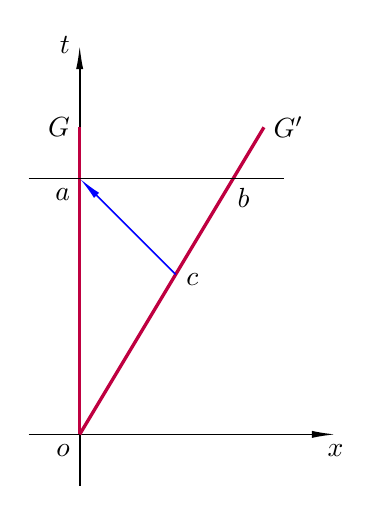
\begin{tikzpicture}[scale=1.3]
			\node[below] (x) at (2.5,0) {$x$};
			\node[left] (t) at (0,3.8) {$t$};
			\node[below left] (O) at (0,0) {$o$};
			\node[left] (G) at (0,3) {$G$};
			\node[right] (g) at (1.8,3) {$G^\prime$};
			\node[below left] (tau) at (0,2.5) {$a$};
			\node[below] (b) at (1.6,2.5) {$b$};
			\node[below] (c) at (1.1,1.6625) {$c$};
			\draw[semithick,\myarrow] (-0.5,0) -- (2.5,0);
			\draw[semithick,\myarrow] (0,-0.5) -- (0,3.8);
			\draw[very thick,purple] (0,0) -- (0,3);
			\draw[very thick,purple] (0,0) -- (1.8,3);
			\draw (-0.5,2.5) -- (2,2.5);
			\draw[semithick,blue,\myarrow] (0.938,1.562) -- (0,2.5);
			\end{tikzpicture}
			\caption{题1解答图}
		\end{figure}
	
	    \begin{enumerate}
	    	\item[(a)] 易知 $b$点的$x$坐标为$0.6\tau$,于是 $b$ 点 $G^\prime$ 的固有时为 \[\tau^\prime = \sqrt{1-0.6^2} \tau = 0.8 \tau = \SI{4}{\micro\second}.\]
	    	\item[(b)] 易求得$b$点在${t,x}$坐标系下的坐标为 $\displaystyle \left( \frac{3}{8} \tau ,\frac{5}{8} \tau \right)$,于是$c$点$G'$的固有时为 \[ \tau^{\prime\prime} = \sqrt{\left(\frac{5}{8}\right)^2-\left(\frac{3}{8}\right)^2} \tau = \frac{\tau}{2} = \SI{2.5}{\micro\second}. \]
	    \end{enumerate}
	\end{jie}
	
	\item 远方星体以$0.8 c $的速率(匀速直线地)离开我们,我们测得它辐射来的闪光按$5$昼夜的周期变化。用时空图求星上观者测得的闪光周期。
	
	\begin{jie}
		如图:
		
		\begin{figure}[htb]
			\centering
			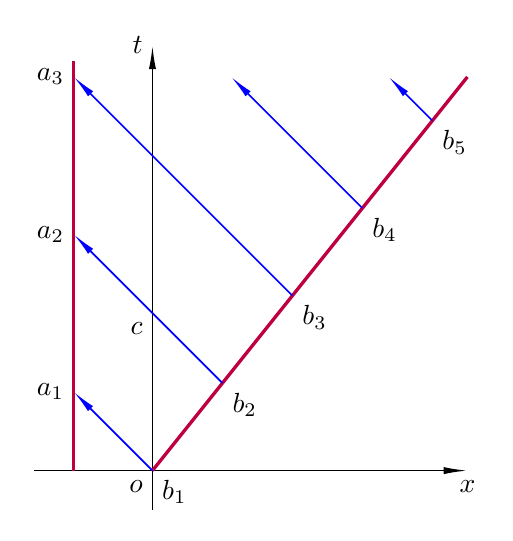
\begin{tikzpicture}
			\node[below] (x) at (5,0) {$x$};
			\node[left] (t) at (1,5.4) {$t$};
			\node[below left] (O) at (1,0) {$o$};
			\node[left] (a1) at (0,1) {$a_1$};
			\node[left] (a2) at (0,3) {$a_2$};
			\node[left] (a3) at (0,5) {$a_3$};
			\node[below right] (b1) at (1,0) {$b_1$};
			\node[below left] (c) at (1,2) {$c$};
			\draw[semithick,\myarrow] (-0.5,0) -- (5,0);
			\draw[semithick,\myarrow] (1,-0.5) -- (1,5.4);
			\draw[very thick,purple] (0,0) -- (0,5.2);
			\draw[very thick,purple] (1,0) -- (5,5);
			\draw[semithick,blue,\myarrow] (1.8889,1.1111) node[below right,black] {$b_2$} -- (0,3);
			\draw[semithick,blue,\myarrow] (1,0) -- (0,1);
			\draw[semithick,blue,\myarrow] (2.7778,2.2222) node[below right,black] {$b_3$} -- (0,5);
			\draw[semithick,blue,\myarrow] (3.6667,3.3333) node[below right,black] {$b_4$} -- (2,5);
			\draw[semithick,blue,\myarrow] (4.5556,4.4444) node[below right,black] {$b_5$} -- (4,5);
			\end{tikzpicture}
			\caption{题2解答图}
		\end{figure}
	
	    记$c$点坐标为$\left(0,\tau\right)$,其中$\tau=\SI{5}{\day}$,则可算得$b_2$点坐标为 $\displaystyle \left(\frac{4}{9},\frac{5}{9}\right) \tau$,于是$b_1$到$b_2$星上观者经过的固有时$\displaystyle \tau^{\prime} = \sqrt{5^2-4^2} \frac{\tau}{9} = \frac{\tau}{3} = \frac{5}{3} \,\si{\day}.$
	\end{jie}
	
	\item 把~\hyperlink{6-20}{图6-20}~的 $oa$ 段和 $oe$ 段线长分别记作 $\tau$ 和 $\tau^\prime$ 。(a) 用两钟的相对速率 $u$ 表出 $\tau^\prime/\tau$ ;(b) 在 $u=0.6c$ 和 $u=0.8c$ 两种情况下求出 $\tau^\prime/\tau$ 的数值。
	
	\begin{figure}[htb]
		\centering
		\begin{tikzpicture}
		\draw[very thick,purple] (0,0) node[left,black] {$o$} -- (0,-5);
		\draw[very thick,purple] (0,0) -- (2,-5);
		\node[above left] (a) at (0,-2) {$a$};
		\draw[semithick,domain=-1.732:1.732,variable=\t,range=0:4, smooth] plot ({2*\t},{-2*sqrt(\t*\t+1)});
		\draw[semithick,blue,\myarrow] (1.333,-3.333) node[below right,black] {$e$} -- (0,-2);
		\node (jz) at (-2,-3) {\colorbox{white}{校准曲线}};
		\node[above,rotate=90] (c) at (0,-3.5) {$C$钟(观者$G$)};
		\node (cc) at (1,-0.9) {$C'$钟};
		\end{tikzpicture}
		\caption{正文图6-20}\hypertarget{6-20}{}
	\end{figure}
    
    \begin{jie}
    	\begin{enumerate}
    		\item[(a)] 如图,记 $t=of$,
    		\begin{equation}
    		\frac{\tau'}{\tau} = \frac{\sqrt{t^2-u^2 t^2}}{t-ut} = \sqrt{\frac{1+u}{1-u}}.
    		\end{equation}
    		
    		\begin{figure}[htb]
    			\centering
    			\begin{tikzpicture}
    			\draw[very thick,purple] (0,0) node[left,black] {$o$} -- (0,-5);
    			\draw[very thick,purple] (0,0) -- (2,-5);
    			\node[above left] (a) at (0,-2) {$a$};
    			\draw[semithick,domain=-1.732:1.732,variable=\t,range=0:4, smooth] plot ({2*\t},{-2*sqrt(\t*\t+1)});
    			\draw[semithick,blue,\myarrow] (1.333,-3.333) node[below right,black] {$e$} -- (0,-2);
    			\draw[semithick] (1.333,-3.333) -- (0,-3.333) node[below right] {$f$} ;
    			\node (jz) at (-2,-3) {\colorbox{white}{校准曲线}};
    			\node[above,rotate=90] (c) at (0,-3.5) {$C$钟(观者$G$)};
    			\node (cc) at (1,-0.9) {$C'$钟};
    			\end{tikzpicture}
    			\caption{题3解答图}\hypertarget{t4}{}
    		\end{figure}
    	
    	    \item[(b)] 将 $u=0.6$ 和 $u=0.8$ 代入,分别得 $\dfrac{\tau'}{\tau}$ 为 $2$ 和 $3$。
    	\end{enumerate}
    \end{jie}
    
    \item 惯性质点 $A,B,C$ 排成一条直线并沿此线相对运动(见~\hyperlink{t5}{图 6.5}),相对速率 $u_{BA}=0.6 c$ , $u_{CA}=0.8 c$ ,$A,B$ 所在惯性系各为 $\mathscr{R}_A$ 和 $\mathscr{R}_B$。设 $\mathscr{R}_B$ 系认为(测得)$C$ 走了 $\SI{60}{m}$,画出时空图并求 $\mathscr{R}_A$ 认为(测得)这一过程的时间。
    
    \begin{figure}[htb]
    	\centering
    	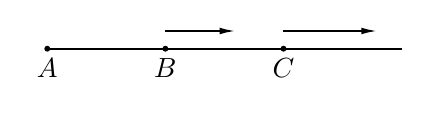
\begin{tikzpicture}[scale=1.5]
    	\filldraw (0,0) circle (0.02cm);
    	\filldraw (1,0) circle (0.02cm);
    	\filldraw (2,0) circle (0.02cm);
    	\draw[semithick] (0,0) node[below] {$A$} -- (1,0) node[below] {$B$} -- (2,0) node[below] {$C$} -- (3,0);
    	\draw[thick,-{Latex[length=6pt,width'=0pt 0.4]}] (1,0.15) -- (1.6,0.15);
    	\draw[thick,-{Latex[length=6pt,width'=0pt 0.4]}] (2,0.15) -- (2.8,0.15);
    	\end{tikzpicture}
    	\caption{题4用图}\hypertarget{t5}{}
    \end{figure}
    
    \begin{jie}
    	如图
    	
    	\begin{figure}[htb]
    		\centering
    		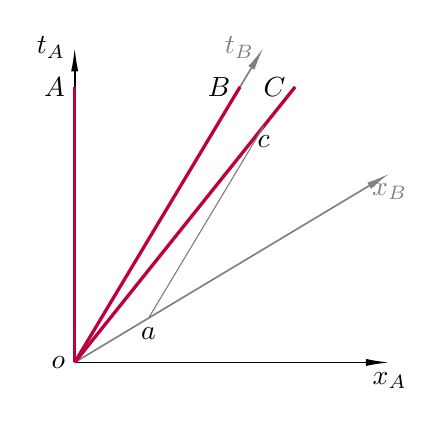
\begin{tikzpicture}
    		\draw[semithick,\myarrow] (0,0) -- (4,0);
			\draw[semithick,\myarrow] (0,0) -- (0,4);
			\draw[semithick,gray,\myarrow] (0,0) -- (2.4,4);
			\draw[semithick,gray,\myarrow] (0,0) -- (4,2.4);
			\node[left] (o) at (0,0) {$o$};
			\node[left] (tA) at (0,4) {$t_A$};
			\node[below] (xA) at (4,0) {$x_A$};
			\node[left,gray] (tB) at (2.4,4) {$t_B$};
			\node[below,gray] (xB) at (4,2.4) {$x_B$};
    		\draw[very thick,purple] (0,0) -- (0,3.5);
    		\draw[very thick,purple] (0,0) -- (2.1,3.5);
			\draw[very thick,purple] (0,0) -- (2.8,3.5);
			\node[left] (A) at (0,3.5) {$A$};
			\node[left] (B) at (2.1,3.5) {$B$};
			\node[left] (C) at (2.8,3.5) {$C$};
			\draw[gray] (0.9375,0.5625) -- (2.4,3);
			\node[below] (c) at (2.4,3) {$c$};
			\node[below] (D) at (0.9375,0.5625) {$a$};
			\end{tikzpicture}
			\caption{题4解答图}
    	\end{figure}
	\end{jie}
	
	$oa$ 段长 $\displaystyle l=\SI{60}{\meter}$,则可算得 $a$ 的坐标为 $\displaystyle \left( \frac{5}{4} , \frac{3}{4} \right) l$,由 $ac$ 的斜率为 $\displaystyle \frac{1}{0.6 c}$,$oc$ 的斜率为 $\displaystyle \frac{1}{0.8c}$ 可求得 $c$ 点坐标为 $\displaystyle \left(\frac{16}{5},\frac{4}{c} \right) l$,即 $oc$ 在 $\mathscr{R}_A$ 看来的时间为 $\displaystyle \frac{4l}{c} = \frac{240}{299792458} \mathrm{m}$。

	\item $A,B$ 是同一惯性系的两个惯性观者,他们互相发射中子,每一中子以相对速率 $0.6 c$ 离开中子枪。设 $B$ 测得 $B$ 枪的中子发射速率为 $\SI{e4}{s^{-1}}$ (即每秒发射 $10^4$ 个),求 $A$ 所发中子(根据中子自己的标准钟)

	\item 暂略。

	\item 暂略。

	\item 暂略。

	\item 暂略。

	\item 暂略。

	\item 暂略。

	\item 试证命题 6-3-4.

	\begin{zm}
		命题6-3-4如下
		\begin{yl}{Thm}
			质点世界线上各点的4加速 $\tensor{A}{^a}$ 与 4 速 $\tensor{U}{^a}$ 正交,即 $\tensor{A}{^a} \tensor{U}{_a} = \tensor{\eta}{_a_b} \tensor{A}{^a} \tensor{U}{^b} =0$。
		\end{yl}
		\begin{yl}{Prf}
			\begin{equation*}
				\begin{split}
					\tensor{U}{_a}\tensor{A}{^a} &= \tensor{U}{_a} \tensor{U}{^b} \Partial{b} \tensor{U}{^a} \\
					&= \frac{1}{2} \tensor{U}{^b} \Partial{b} \left( \tensor{U}{_a} \tensor{U}{^a} \right)\\
					&=0.
				\end{split}
			\end{equation*}
		\end{yl}
	\end{zm}

	\item 设观者世界线为 $t\sim x$ 面内的双曲线 $G$ (见\hyperlink{t6}{图 6.7}),图中 $K$ 为已知,$\tensor{A}{^a}$ 为观者的 4 加速,求 $\tensor{A}{^a} \tensor{A}{_a}$(结论是 $\tensor{A}{^a} \tensor{A}{_a}$ 为常数,因此 $G$ 称为匀加速运动观者\footnote{或称 Rindler 观者——笔者注}。请注意这指的是4加速。)

	\begin{figure}[htb]
		\centering
		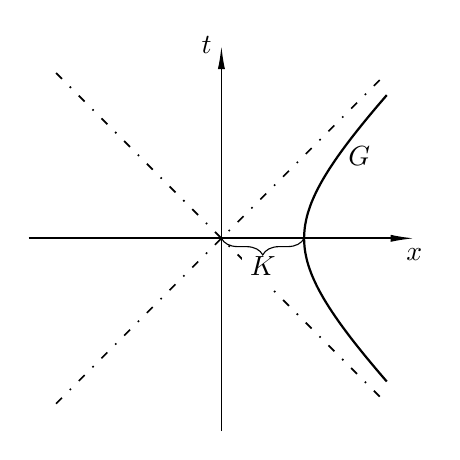
\begin{tikzpicture}[decoration={brace,amplitude=6},scale=0.7]
			\draw[semithick,\myarrow] (-3.5,0) -- (3.5,0);
			\draw[semithick,\myarrow] (0,-3.5) -- (0,3.5);
			\node[left] (t) at (0,3.5) {$t$};
			\node[below] (x) at (3.5,0) {$x$};
			\draw[semithick,loosely dash dot] (-3,-3) -- (3,3);
			\draw[semithick,loosely dash dot] (-3,3) -- (3,-3);
			\draw[domain=-1.732:1.732,variable=\t,range=0:4, smooth,thick] plot ({1.5*sqrt(\t*\t+1)},{1.5*\t});
			\node (G) at (2.5,1.5) {$G$};
			\node (K) at (0.75,-0.5) {\colorbox{white}{$K$}};
			\draw[decorate] (1.5,0) -- (0,0);
		\end{tikzpicture}
		\caption{习题13用图}\hypertarget{t6}{}
	\end{figure}

	\begin{jie}
		由图知此双曲线的参数为 $a=b=K$ ,可写出双曲线方程为
		\begin{equation*}
			x^2-t^2=K^2,
		\end{equation*}
		两边对固有时求导,
		\begin{gather*}
			2x \dv{x}{\tau} - 2t \dv{t}{\tau} = 0,\\
			\dv{x}{\tau} = \frac{t}{x} \dv{t}{\tau},
		\end{gather*}
		而
		\begin{equation*}
			\begin{split}
				\tensor{Z}{^a} &= \dv{t}{\tau} \tensor{\left(\pdv{t}\right)}{^a} + \dv{x}{\tau} \tensor{\left(\pdv{x}\right)}{^a}
			\end{split}
		\end{equation*}
		是归一的,则
		\begin{equation*}
			\begin{split}
				\left(\dv{x}{\tau} \right)^2 - \left( \dv{t}{\tau} \right)^2 &= \left[ \left(\frac{t}{x}\right)^2 - 1 \right] \left( \dv{t}{\tau} \right)^2\\
				&= - \left( \frac{K}{x} \dv{t}{\tau} \right)^2\\
				&= -1,
			\end{split}
		\end{equation*}
		\begin{equation*}
			\implies \frac{1}{x} \dv{t}{\tau} = \frac{1}{t} \dv{x}{\tau} = \frac{1}{K},
		\end{equation*}
		于是4速又可改写为
		\begin{equation*}
			\tensor{Z}{^a} = \frac{1}{K} \left[ x \tensor{\left(\pdv{t}\right)}{^a} + t \tensor{\left(\pdv{x}\right)}{^a} \right],
		\end{equation*}
		故
		\begin{equation*}
			\begin{split}
				\tensor{A}{^a} &= \dv{\tensor{Z}{^a}}{\tau}\\
				&= \frac{1}{K} \left[ \dv{x}{\tau} \tensor{\left(\pdv{t}\right)}{^a} + \dv{t}{\tau} \tensor{\left(\pdv{x}\right)}{^a} \right]\\
				&= \frac{1}{K^2} \left[ t \tensor{\left(\pdv{t}\right)}{^a} + x \tensor{\left(\pdv{x}\right)}{^a} \right],\\
				\tensor{A}{_a} \tensor{A}{^a} &= \frac{1}{K^4} \left( x^2 - t^2 \right)\\
				&= \frac{1}{K^2}.
			\end{split}
		\end{equation*}
	\end{jie}

	\item 试证命题6-6-2.

	\begin{zm}
		命题6-6-2如下
		\begin{yl}{Thm}
			设惯性系 $\mathscr{R}$ 和 $\mathscr{R}^\prime$ 由洛伦兹变换
			\begin{equation*}
				t = \gamma \left( t^\prime + v x^\prime \right) \qc x = \gamma \left( x^\prime + v t^\prime \right) \qc y = y^\prime \qc z = z^\prime
			\end{equation*}
			相联系,则两者测同一电磁场 $\tensor{F}{_a_b}$ 所得值 $\left( \myvec{E},\myvec{B} \right)$ 和 $\left( \myvec{E}^\prime , \myvec{B}^\prime \right)$ 有如下关系:
			\begin{align*}
				E_1^\prime &= E_1, & E_2^\prime &= \gamma \left( E_2 - v B_3 \right), & E_3^\prime &= \gamma \left( E_3 + v B_2 \right);\\
				B_1^\prime &= B_1, & B_2^\prime &= \gamma \left( B_2 + v E_3 \right), & B_3^\prime &= \gamma \left( B_3 - v E_2 \right).
			\end{align*}
		\end{yl}
		\begin{yl}{Prf}
			记矩阵 $\Lambda$ 为
			\begin{equation*}
				\left[ \tensor{\Lambda}{^\mu_\nu} \right] = \left[ \pdv{x^\mu}{x^{\prime\nu}} \right] = \mqty( \mqty{ \gamma & \gamma v \\ \gamma v & \gamma }  & \mqty{\zmat{2}{2}} \\ \mqty{\zmat{2}{2}} & \mqty{\imat{2}} ),
			\end{equation*}
			则易知
			\begin{equation*}
				\left[ \tensor{\left(\Lambda^{-1}\right)}{^\mu_\nu} \right] = \left[ \pdv{x^{\prime\mu}}{x^{\nu}} \right] = \mqty( \mqty{ \gamma & - \gamma v \\ - \gamma v & \gamma }  & \mqty{\zmat{2}{2}} \\ \mqty{\zmat{2}{2}} & \mqty{\imat{2}} ),
			\end{equation*}
			而根据张量变换律
			\begin{equation*}
				\begin{split}
					\tensor{{F^\prime}}{^\mu_\nu} &= \pdv{x^{\prime\mu}}{x^\sigma} \pdv{x^\rho}{x^{\prime\nu}} \tensor{F}{^\sigma_\rho}\\
					&= \tensor{\left(\Lambda^{-1}\right)}{^\mu_\sigma} \tensor{F}{^\sigma_\rho} \tensor{\Lambda}{^\rho_\nu},
				\end{split}
			\end{equation*}
			于是有矩阵等式
			\begin{equation*}
				\left[F^\prime\right] = \Lambda^{-1} \left[F\right] \Lambda,
			\end{equation*}
			其中 $\left[F\right]$ 表示 $\tensor{F}{^\mu_\nu}$ 排成的矩阵
			\begin{equation*}
				\left[F\right] = \mqty( 0 & E_1 & E_2 & E_3 \\ E_1 & 0 & B_3 & -B_2 \\ E_2 & -B_3 & 0 & B_1 \\ E_3 & B_2 & -B_1 & 0 ),
			\end{equation*}
			于是经过简单的矩阵乘法算得
			\begin{equation*}
				\left[ F^\prime \right] = \mqty( 0 & E_1 & \gamma \left( E_2 - v B_3 \right) & \gamma \left( E_3 + v B_2 \right) \\ E_1 & 0 & \gamma \left( B_3 - v E_2 \right) & - \gamma \left( B_2 + v E_3 \right) \\ \gamma \left( E_2 - v B_3 \right) & - \gamma \left( B_3 - v E_2 \right) & 0 & B_1 \\ \gamma \left( E_3 + v B_2 \right) & \gamma \left( B_2 + v E_3 \right) & -B_1 & 0 ),
			\end{equation*}
			可以直接读出
			\begin{align*}
				E_1^\prime &= E_1, & E_2^\prime &= \gamma \left( E_2 - v B_3 \right), & E_3^\prime &= \gamma \left( E_3 + v B_2 \right);\\
				B_1^\prime &= B_1, & B_2^\prime &= \gamma \left( B_2 + v E_3 \right), & B_3^\prime &= \gamma \left( B_3 - v E_2 \right).
			\end{align*}
		\end{yl}
	\end{zm}
	
\end{xiti}
	% !TeX root = ../document.tex

\chapter{广义相对论基础}
\begin{xiti}
	\item 试证弯曲时空麦氏方程 $\tensor{\nabla}{^a} \tensor{F}{_a_b} = - 4\pi \tensor{J}{_b}$ 蕴含电荷守恒定律,即 $\Nabla{a} \tensor{J}{^a} = 0$ 。注:$\tensor{\nabla}{^a} \tensor{F}{_a_b} = - 4\pi \tensor{J}{_b}$ 等价于式 (7-2-8) 而非 (7-2-9) ,故本题表明式 (7-2-8) 而非式 (7-2-9) 可推出电荷守恒。
	
	\begin{zm}
		\begin{equation*}
		-4 \pi \Nabla{a} \tensor{J}{^a} = \Nabla{a} \Nabla{b} \tensor{F}{^b^a} = 0.
		\end{equation*}
	\end{zm}
    
    \item 试证 $\displaystyle \Fd{\tensor{\omega}{_a}} = \Dd{\tensor{\omega}{_a}} + \left(\tensor{A}{_a} \wedge \tensor{Z}{_b}\right) \tensor{\omega}{^b} \quad \forall \tensor{\omega}{_a} \in \F_{G}(0,1).$
    
    \begin{zm}
    	$\forall \tensor{v}{^a} \in \F_{G}(1,0),$
    	\begin{align*}
    	    \tensor{v}{^a} \Fd{\tensor{\omega}{_a}} &= \Fd{\left(\tensor{v}{^a}\tensor{\omega}{_a}\right)} - \tensor{\omega}{_a} \Fd{\tensor{v}{^a}}\\
    	    &= \tensor{v}{^a} \Dd{\tensor{\omega}{_a}} + \tensor{\omega}{_a} \Dd{\tensor{v}{^a}} - \tensor{\omega}{_a} \left( \Dd{\tensor{v}{^a}} + 2 \tensor{A}{^{[a}} \tensor{Z}{^{b]}} \tensor{v}{_b} \right)\\
    	    &= \tensor{v}{^a} \left( \Dd{\tensor{\omega}{_a}} - 2 \tensor{A}{_{[b}} \tensor{Z}{_{a]}} \tensor{\omega}{^b} \right)\\
    	    &= \tensor{v}{^a} \left( \Dd{\tensor{\omega}{_a}} + \tensor{A}{_{a}} \wedge \tensor{Z}{_{b}} \tensor{\omega}{^b} \right).
    	\end{align*}
    \end{zm}
    
    \item 试证费米导数性质3.\label{prob-7.3}
    
    \begin{zm}
    	性质3如下:
    	\begin{Property}
    		若 $\tensor{w}{^a}$ 是 $G(\tau)$ 上的空间矢量场(对线上各点 $\tensor{w}{^a} \tensor{Z}{_a} = 0$ ),则 \[ \Fdd{\tensor{w}{^a}} = \tensor{h}{^a_b} \left( \Ddd{\tensor{w}{^b}} \right), \] 其中 $\tensor{h}{^a_b} = \tensor{g}{_a_b} + \tensor{Z}{_a} \tensor{Z}{_b}$ ,$\tensor{h}{^a_b} = \tensor{g}{^a^c} \tensor{h}{_c_b}$ 是 $G(\tau)$ 上各点的投影映射。
    	\end{Property}
    	\begin{Proof}
    		$\tensor{h}{^a_b} = \tensor{g}{^a^c} \left( \tensor{g}{_c_b} + \tensor{Z}{_c} \tensor{Z}{_b} \right) = \tensor{\delta}{^a_b} + \tensor{Z}{^a} \tensor{Z}{_b},$
    		\begin{align*}
    		\tensor{h}{^a_b} \Dd{\tensor{w}{^b}} &= \left( \tensor{\delta}{^a_b} + \tensor{Z}{^a} \tensor{Z}{_b} \right) \Dd{\tensor{w}{^b}}\\
    		&= \Dd{\tensor{w}{^a}} + \tensor{Z}{^a} \left( \Dd{\left( \tensor{Z}{_b} \tensor{w}{^b} \right)} - \tensor{w}{^b} \Dd{\tensor{Z}{_b}} \right)\\
    		&= \Dd{\tensor{w}{^a}} - \tensor{Z}{^a} \tensor{A}{^b} \tensor{w}{_b}\\
    		&= \Dd{\tensor{w}{^a}} + \left(\tensor{A}{^a} \tensor{Z}{^b} - \tensor{Z}{^a} \tensor{A}{^b}\right) \tensor{w}{_b}\\
    		&= \Fd{\tensor{w}{^a}}.
    		\end{align*}
    	\end{Proof}
    \end{zm}
    
    \item 试证类时线 $G(\tau)$ 上长度不变(且非零)的矢量场必经受时空转动。提示:令 $\tensor{u}{^a} \equiv \Ddd{\tensor{v}{^a}}$,则 $\tensor{u}{_a} \tensor{v}{^a}=0$。先证:无论 $\tensor{v}{_a}\tensor{v}{^a}$ 为零与否,总有 $G(\tau)$ 上矢量场 $\tensor{{v'}}{^a}$ 使 $\tensor{{v'}}{_a} \tensor{v}{^a} = 1$ 。再验证 $\tensor{v}{^a}$ 经受以 $\tensor{\Omega}{_a_b} \equiv 2 \tensor{{v'}}{_{[a}} \tensor{u}{_{b]}}$ 为角速度 2 形式的时空转动。
    
	\begin{zm}
		\begin{enumerate}
			\item 记 $\displaystyle \tensor{u}{^a} = \Dd{\tensor{v}{^a}}$ ,则 $\displaystyle \Dd{\left(\tensor{v}{_a}\tensor{v}{^a}\right)} = 2\tensor{u}{_a} \tensor{v}{^a}=0$ 。
			\item 若 $\tensor{v}{^a} \tensor{v}{_a} \neq 0$,令
			\begin{equation*}
				\tensor{{v'}}{^a} = \frac{\tensor{v}{^a}}{\tensor{v}{^b} \tensor{v}{^b}},
			\end{equation*}
			若 $\tensor{v}{^a} \tensor{v}{_a} = 0$,则 $\tensor{Z}{^a} \tensor{v}{_a}$ 不为零,因为与类时矢量内积为零则为类空矢量。于是定义
			\begin{equation*}
				\tensor{{v'}}{^a} = \frac{\tensor{Z}{^a}}{\tensor{Z}{^b} \tensor{v}{_b}}.
			\end{equation*}
			\item 定义 $\tensor{\Omega}{_a_b} = 2 \tensor{{v'}}{_{[a}} \tensor{u}{_{b]}}$,则
			\begin{equation*}
				- \tensor{\Omega}{^a^b} \tensor{v}{_b} = \tensor{u}{^a} = \Dd{\tensor{v}{^a}},
			\end{equation*}
			故 $\tensor{v}{^a}$ 经受以 $\tensor{\Omega}{_a_b}$ 为角速度 2 形式的时空转动。
		\end{enumerate}
	\end{zm}
	
	\item 设 $\left\{ T,X,Y,Z \right\}$ 为闵氏时空的洛伦兹坐标系,曲线 $G(\tau)$ 的参数表达式为
	\begin{equation*}
		T = A^{-1} \sinh A\tau \qc X = A^{-1} \cosh A\tau \qc Y=Z=0 \qc \text{(其中$A$ 为常数)}
	\end{equation*}
	\begin{enumerate}[label=(\alph*)]
		\item 试证 $G(\tau)$ 是类时双曲线(即图(6-43)\footnote{即本文档图~\hyperlink{t6}{6.13}} 中的 $G$),$\tau$ 是固有时,$A$ 是 $G(\tau)$ 的 4 加速 $\tensor{A}{^a}$ 的长度。
		\item 试证从 $\left\{ T,X,Y,Z \right\}$ 坐标系原点 $o$ 出发的与 $G(\tau)$ 有交的任一半直线 $\mu(s)$ 都与 $G(\tau)$ 正交。
		\item 设(b)中的 $\mu(s)$ 的参数 $s$ 是 $\mu$ 的线长,随着 $\mu(s)$ 取遍所有从 $o$ 出发并与 $G(\tau)$ 有交的半直线,便得 $G(\tau)$ 上的一个空间矢量场 $\tensor{w}{^a} \equiv \tensor{\left( \pdv*{s} \right)}{^a}$,试证 $\tensor{w}{^a}$ 沿 $G(\tau)$ 费移。
		\item 令 $\tensor{Z}{^a} \equiv \tensor{\left( \pdv*{\tau} \right)}{^a}$,选 $\left\{ \tensor{Z}{^a}, \tensor{w}{^a}, \tensor{\left( \pdv*{Y} \right)}{^a}, \tensor{\left( \pdv*{Z} \right)}{^a} \right\}$ 为 $G(\tau)$ 上的正交归一 4 标架场,求出 $G(\tau)$ 的固有坐标系 $\left\{ t, x, y, z \right\}$ 并指出其坐标域。
		
		答: $T=\left( A^{-1} + x \right) \sinh At \qc X= \left( A^{-1} + x \right) \cosh At \qc Y=y \qc Z=z$。

		\item 写出闵氏时空在上述固有坐标系中的线元表达式。计算闵氏度规在该系的克氏符,验证它满足引理 7-4-3,即式 (7-4-10)\footnote{正文 (7-4-10) 为
		\begin{equation*}
			\begin{gathered}
				\ChristoffelSymbol{0}{0}{0} = \ChristoffelSymbol{\sigma}{i}{j} = 0 \qc \ChristoffelSymbol{0}{0}{i} = \ChristoffelSymbol{0}{i}{0} = \ChristoffelSymbol{i}{0}{0} = \tensor{\hat{A}}{_i},\\
				\ChristoffelSymbol{i}{0}{j} = \ChristoffelSymbol{i}{j}{0} = - \tensor{\omega}{^k} \tensor{\varepsilon}{_0_k_i_j} \qc \sigma = 0,1,2,3; \quad i,j,k = 1,2,3.
			\end{gathered}
		\end{equation*}
		}。
	\end{enumerate}

		\begin{zm}
			\begin{enumerate}[label=(\alph*)]
				\item 由 $\cosh^2 x - \sinh^2 x = 1$ 知 $\left( A X \right)^2 - \left( A T \right)^2 = 1$,故这是渐近线为 $T=\pm X$ 的双曲线。
				
				以 $\tau$ 为参数,
				\begin{equation*}
					\tensor{\left( \pdv{\tau} \right)}{^a} = \cosh(A\tau) \tensor{\left( \pdv{T} \right)}{^a} + \sinh(A\tau) \tensor{\left( \pdv{X} \right)}{^a},
				\end{equation*}
				则
				\begin{equation*}
					\tensor{\eta}{_a_b} \tensor{\left( \pdv{\tau} \right)}{^a} \tensor{\left( \pdv{\tau} \right)}{^b} = - \cosh[2](A\tau) + \sinh[2](A\tau) = -1,
				\end{equation*}
				即切矢归一,$\tau$ 为固有时。

				将 $\tensor{\left( \pdv{\tau} \right)}{^a}$ 延拓为
				\begin{equation*}
					\tensor{Z}{^a} = A X \tensor{\left( \pdv{T} \right)}{^a} + A T \tensor{\left( \pdv{X} \right)}{^a},
				\end{equation*}
				容易算得观者四加速为
				\begin{equation*}
					\begin{split}
						\tensor{\hat{A}}{^a} &= \left. \tensor{Z}{^b} \Nabla{b} \tensor{Z}{^a}\right|_{G(\tau)}\\
						&= \left. A^2 T \tensor{\left( \pdv{T} \right)}{^a} + A^2 X \tensor{\left( \pdv{X} \right)}{^a} \right|_{G(\tau)}\\
						&= A \sinh(A\tau) \tensor{\left( \pdv{T} \right)}{^a} + A \cosh(A\tau) \tensor{\left( \pdv{X} \right)}{^a},
					\end{split}
				\end{equation*}
				则
				\begin{equation*}
					\tensor{\eta}{_a_b} \tensor{\hat{A}}{^a} \tensor{\hat{A}}{^b} = A^2 \left( \cosh[2](A\tau) - \sinh[2](A\tau) \right) = A^2,
				\end{equation*}
				即四加速的模长为 $A$。

				\item 与 $G$ 交于 $\tau$ 处的 $\mu$ 的方程为
				\begin{equation*}
					T = \tanh(A\tau) X,
				\end{equation*}
				故其在 $G(\tau)$ 处的切矢正比于
				\begin{equation*}
					\tensor{\left( \pdv{s} \right)}{^a} = \sinh(A\tau)\tensor{\left( \pdv{T} \right)}{^a} + \cosh(A\tau) \tensor{\left( \pdv{X} \right)}{^a},
				\end{equation*}
				可算得
				\begin{equation*}
					\tensor{\left( \pdv{s} \right)}{^a} \tensor{\left( \pdv{\tau} \right)}{_a} = - \cosh(A\tau) \sinh(A\tau) + \cosh(A\tau) \sinh(A\tau) =0.
				\end{equation*}
				\item 在 (b) 中给出的 $\tensor{\left( \pdv*{s} \right)}{^a}$ 已经是归一的,因而就是 $\tensor{w}{^a}$。
				由(b) 和习题~\hyperref[prob-7.3]{3},知
				\begin{equation*}
					\begin{split}
						\Fd{\tensor{w}{^a}} &= \tensor{h}{^a_b} \Dd{\tensor{w}{^b}}\\
						&= \tensor{h}{^a_b} \tensor{Z}{^c} \Nabla{c} \tensor{w}{^b}\\
						&= \tensor{h}{^a_b} \left( A \cosh(A\tau) \tensor{\left( \pdv{T} \right)}{^b} + A \sinh(A\tau) \tensor{\left( \pdv{X} \right)}{^b} \right)\\
						&= A \tensor{h}{^a_b} \tensor{Z}{^b}\\
						&= 0,
					\end{split}
				\end{equation*}
				其中 $\tensor{Z}{^a} = \tensor{\left( \pdv*{\tau} \right)}{^a}$,故 $\tensor{w}{^a}$ 沿 $G(\tau)$ 费移。
				\item 以 $G(0)$ 为坐标原点,$\left\{ t,0,0,0\right\}$ 对应的点为 $G(t)$,即
				\begin{equation*}
					T= A^{-1} \sinh A t \qc X= A^{-1} \cosh A t \qc Y = Z =0,
				\end{equation*}
				而此点处
				\begin{equation*}
					\begin{split}
						&x\tensor{w}{^a} + y \tensor{\left( \pdv{Y} \right)}{^a} + z \tensor{\left( \pdv{Z} \right)}{^a}\\
						={}& x \sinh(At) \tensor{\left( \pdv{T} \right)}{^a} + x \cosh(At) \tensor{\left( \pdv{X} \right)}{^a} + y \tensor{\left( \pdv{Y} \right)}{^a} + z \tensor{\left( \pdv{Z} \right)}{^a},
					\end{split}
				\end{equation*}
				沿此矢量决定的测地线(直线)走参数为1的距离,即
				\begin{equation*}
					\Delta T = x \sinh(At) \qc \Delta X = x \cosh(At) \qc \Delta Y = y \qc \Delta Z = z \tensor{\left( \pdv{Z} \right)}{^a},
				\end{equation*}
				故 $\left\{ t,x,y,z \right\}$ 对应的点为
				\begin{equation}
					T=\left( A^{-1} + x \right) \sinh At \qc X= \left( A^{-1} + x \right) \cosh At \qc Y=y \qc Z=z. \label{eq-txyz2TXYZ}
				\end{equation}
				\item 计算得
				\begin{equation*}
					\begin{split}
						\dd{s}^2 ={}& - \dd{T}^2 + \dd{X}^2 + \dd{Y}^2 + \dd{Z}^2\\
						={}& - \left[ \left( 1 + A x \right) \cosh(A t) \dd{t} + \sinh(A t) \dd{x} \right]^2\\
						&{}+ \left[ \left( 1 + A x \right) \sinh(A t) \dd{t} + \cosh(A t) \dd{x} \right]^2 + \dd{y}^2 + \dd{z}^2\\
						={}& - \left( 1+ A x \right)^2 \dd{t}^2 + \dd{x}^2 + \dd{y}^2 + \dd{z}^2,
					\end{split}
				\end{equation*}
				容易算得非零克氏符为
				\begin{equation*}
					\ChristoffelSymbol{t}{t}{x} = \ChristoffelSymbol{t}{x}{t} = \frac{A}{1+A x} \qc \ChristoffelSymbol{x}{t}{t} = A \left( 1+Ax \right),
				\end{equation*}
				在线上时
				\begin{equation*}
					\ChristoffelSymbol{t}{t}{x} = \ChristoffelSymbol{t}{x}{t} =  \ChristoffelSymbol{x}{t}{t} = A,
				\end{equation*}
				% 而观者的四加速为
				% \begin{equation*}
				% 	\begin{split}
				% 		\tensor{\hat{A}}{^a} &= \tensor{Z}{^b} \Nabla{b} \tensor{Z}{^a}\\
				% 		&= \left( A X \tensor{\left( \pdv{T} \right)}{^b} + A T \tensor{\left( \pdv{X} \right)}{^b} \right) \Nabla{b} \left( A X \tensor{\left( \pdv{T} \right)}{^a} + A T \tensor{\left( \pdv{X} \right)}{^a} \right)\\
				% 		&= A^2 X \tensor{\left( \pdv{X} \right)}{^a} + A^2 T \tensor{\left( \pdv{T} \right)}{^a},
				% 	\end{split}
				% \end{equation*}
				对~\eqref{eq-txyz2TXYZ} 反解得坐标变换
				\begin{equation*}
					t = A^{-1} \tanh[-1](\frac{T}{X}) \qc x = \sqrt{X^2 - T^2} - A^{-1} \qc y = Y \qc z = Z,
				\end{equation*}
				故
				\begin{equation*}
					\begin{split}
						\tensor{\left( \pdv{T} \right)}{^a} &= \pdv{t}{T} \tensor{\left( \pdv{t} \right)}{^a} + \pdv{x}{T} \tensor{\left( \pdv{x} \right)}{^a}\\
						&= \frac{X}{A\left( X^2 - T^2 \right)} \tensor{\left( \pdv{t} \right)}{^a} - \frac{T}{\sqrt{X^2 - T^2}} \tensor{\left( \pdv{x} \right)}{^a}\\
						&= \frac{\cosh At}{1+Ax} \tensor{\left( \pdv{t} \right)}{^a} - \sinh(At) \tensor{\left( \pdv{x} \right)}{^a},\\
						\tensor{\left( \pdv{X} \right)}{^a} &= \pdv{t}{X} \tensor{\left( \pdv{t} \right)}{^a} + \pdv{x}{X} \tensor{\left( \pdv{x} \right)}{^a}\\
						&= \frac{T}{A\left( T^2 - X^2 \right)} \tensor{\left( \pdv{t} \right)}{^a} + \frac{X}{\sqrt{X^2 - T^2}} \tensor{\left( \pdv{x} \right)}{^a}\\
						&= - \frac{\sinh At}{1+Ax} \tensor{\left( \pdv{t} \right)}{^a} + \cosh(At) \tensor{\left( \pdv{x} \right)}{^a},
					\end{split}
				\end{equation*}
				故
				\begin{equation*}
					\begin{split}
						\tensor{\hat{A}}{^a} ={}& A^2 X \tensor{\left( \pdv{X} \right)}{^a} + A^2 T \tensor{\left( \pdv{T} \right)}{^a}\\
						={}& A \left( 1 + A x \right) \cosh(At) \left( - \frac{\sinh At}{1+Ax} \tensor{\left( \pdv{t} \right)}{^a} + \cosh(At) \tensor{\left( \pdv{x} \right)}{^a} \right)\\
						&{} + A\left( 1+Ax \right) \sinh(At) \left( \frac{\cosh At}{1+Ax} \tensor{\left( \pdv{t} \right)}{^a} - \sinh(At) \tensor{\left( \pdv{x} \right)}{^a} \right)\\
						={}& A \left( 1+ Ax \right) \tensor{\left( \pdv{x} \right)}{^a},
					\end{split}
				\end{equation*}
				在线上有
				\begin{equation*}
					\tensor{\hat{A}}{^a} = A \tensor{\left( \pdv{x} \right)}{^a},
				\end{equation*}
				满足引理,证毕。
			\end{enumerate}
		\end{zm}

	\item 设 $G$ 是质点 $L$ 在 $p\in L$ 的瞬时静止自由下落观者(即 $G$ 的 4 速 $\tensor{Z}{^a}$ 与 $L$ 的 4 速 $\tensor{U}{^a}$ 在 $p$ 点相切),$\tensor{A}{^a}	$ 是 $L$ 在 $p$ 点的 4 加速,$\tensor{a}{^a}	$ 是 $L$ 在 $p$ 点相对于 $G$ 的 3 加速[由式 (7-4-3)\footnote{正文式 (7-4-3) 为
	\begin{equation*}
		\tensor{a}{^a} := \left[ \dv[2]{x^i(t)}{t} \right] \tensor{\left( \pdv{x^i} \right)}{^a}.
	\end{equation*}}定义],试证 $\tensor{a}{^a} = \tensor{A}{^a}$。\\
	注:本题可视为命题 6-3-6 在弯曲时空的推广。

		\begin{zm}
			记 $G(t)$ 的固有坐标系为 $\left\{ t,x,y,z \right\}$。在 $p$ 点,有 $\tensor{U}{^a} = \tensor{Z}{^a} = \tensor{\left( \pdv{t} \right)}{^a}$。对 $\tensor{U}{^a}$ 做分解,有
			\begin{equation*}
				\tensor{U}{^a} = \tensor{\left( \pdv{\tau_L} \right)}{^a} = \dv{t}{\tau_L} \tensor{\left( \pdv{t} \right)}{^a} + \dv{x^i}{\tau_L} \tensor{\left( \pdv{x^i} \right)}{^a} = \gamma \tensor{Z}{^a} + \gamma \tensor{u}{^a},
			\end{equation*}
			则
			\begin{equation*}
				\gamma|_p = 1 \qc \tensor{u}{^a}|_{p} = 0,
			\end{equation*}
			而
			\begin{equation*}
				\begin{split}
					\tensor{A}{^a}|_p &= \left( \tensor{Z}{^b} \Nabla{b} \tensor{U}{^a} \right)_p\\
					&= \left( \Partial{0} \tensor{U}{^a} + \ChristoffelSymbol{0}{a}{b} \tensor{U}{^b} \right)_p\\
					&= \Partial{0} \tensor{U}{^a} |_p\\
					&= \dv{\gamma}{t} \tensor{Z}{^a} + \dv{\gamma}{t} \tensor{u}{^a} + \gamma \dv{\tensor{u}{^a}}{t}\\
					&= \dv{\tensor{u}{^a}}{t},
				\end{split}
			\end{equation*}
			其中最后一步用到 $\left.\dv{\gamma}{t}\right|_p = 0$,这是因为 $\gamma = - \tensor{U}{^a} \tensor{Z}{_a} \leqslant 1$,故在 $p$ 点 $\gamma|_p=1$ 取到了极值。而 $\dv{\tensor{u}{^a}}{t}$ 就是 $\tensor{a}{^a}$。
		\end{zm}

	\item 度规 $\tensor{g}{_a_b}$ 叫 \textbf{里奇平直} 的,若 $\tensor{g}{_a_b}$ 的里奇张量为零。试证 $\tensor{g}{_a_b}$ 是真空爱因斯坦方程的解的充要条件是 $\tensor{g}{_a_b}$ 是里奇平直的。
	
		\begin{zm}
			真空爱因斯坦方程为 $\tensor{R}{_a_b} - \frac{1}{2} R \tensor{g}{_a_b} = 0$。
			\begin{enumerate}
				\item 充分性:若 $\tensor{R}{_a_b} = 0$,则取迹得 $R=0$,故满足真空场方程。
				\item 必要性:设 $\tensor{g}{_a_b}$ 满足真空场方程,即 $\tensor{R}{_a_b} - \frac{1}{2} R \tensor{g}{_a_b} = 0$,取迹得
				\begin{equation*}
					R - 2 R = -R = 0,
				\end{equation*}
				故
				\begin{equation*}
					\tensor{R}{_a_b} - \frac{1}{2} R \tensor{g}{_a_b} = \tensor{R}{_a_b} = 0,
				\end{equation*}
				故里奇平直。
			\end{enumerate}
		\end{zm}
    
\end{xiti}
	% !TeX root = ../document.tex

\chapter{爱因斯坦方程的求解}

\begin{xiti}
    \item 试证命题 8-1-1。
    
    \begin{zm}
        正文命题8-1-1为
        \begin{Proposition}
            设 $\tensor{\xi}{^a} = \tensor{\left( \pdv*{t} \right)}{^a} $ 是 Killing 矢量场,$\Sigma_0 = \left\{ p \in M \mid t(p) = 0 \right\}$ 是处处与 $\tensor{\xi}{^a}$ 正交的超曲面,则 超曲面 $\Sigma_{t_1} = \left\{ p \in M \mid t(p) = t_1 \right\}$ 也处处与 $\tensor{\xi}{^a}$ 正交。
        \end{Proposition}

        \begin{Proof}
            设矢量场 $\tensor{\xi}{^a}$ 生成的单参微分同胚群 为 $\phi_t$,则 $\Sigma_{t_1} = \phi_{t_1} \left[ \Sigma_0 \right]$,任取 $p \in \Sigma_0$,$q = \phi_{t_1}(p) \in \Sigma_{t_1}$,以及 $q$ 点处 $\Sigma_{t_1}$ 的任意切矢量 $\tensor{v}{^a} \in \TB[q]{\Sigma_{t_1}}$,则 $\tensor{u}{^a} = \left( \phi_{-t_1} \right)_* \tensor{v}{^a} \in \TBx[p]{\Sigma_0}$,故
            \begin{equation*}
                \begin{split}
                    \left.\tensor{g}{_a_b}\right|_{q} \tensor{v}{^a} \left.\tensor{\xi}{^b}\right|_q &= \left( \phi_{t_1} \right)_* \left( \left. \tensor{g}{_a_b} \right|_{p} \right) \tensor{v}{^a} \left( \phi_{t_1} \right)_* \left( \left. \tensor{\xi}{^a} \right|_p \right)\\
                    &= \left( \phi_{t_1} \right)_* \left( \left. \tensor{g}{_a_b} \right|_p \tensor{u}{^a} \left. \tensor{\xi}{^b} \right|_p \right)\\
                    &= \left( \phi_{t_1} \right)_* 0\\
                    &= 0,
                \end{split}
            \end{equation*}
            故 $\Sigma_{t_1}$ 也与 $\tensor{\xi}{^a}$ 正交。
        \end{Proof}  
    \end{zm}
    
    \item 设 $\gamma(r)$ 是图 8-6 中 $\Sigma_{t}$ 上从 $p_1$ 到 $p_2$ 的、$\theta$ 和 $\varphi$ 都为常数的曲线(以径向坐标 $r$ 为曲线参数),试证 $\gamma(r)$ 是(非仿射参数化的)测地线。提示:用式(5-7-2)。
    
    \begin{figure}[htpb!]
        \centering
        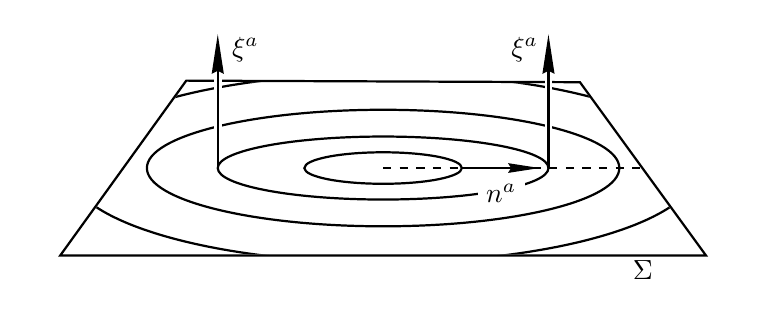
\begin{tikzpicture}[thick]
            \draw (0,0) ellipse [x radius=1,y radius=.2];
            \draw (0,0) ellipse [x radius=2.1, y radius=0.4];
            \draw (0,0) ellipse [x radius=3, y radius=0.74];
            \draw (0,0) ellipse [x radius=4, y radius=1.2];
            \filldraw[fill=white,color=white] (-4.5,1.5) -- (4.5,1.5) -- (4.5,-1.5) -- (-4.5,-1.5) -- cycle (-2.5,1.11) -- (-4.1,-1.11) -- (4.1,-1.11) -- (2.5,1.09) -- cycle;
            \draw (-2.5,1.11) -- (-4.1,-1.11) -- (4.1,-1.11) -- (2.5,1.09) -- cycle;
            \draw[dashed] (0,0) -- (3.3,0);
            \draw[-{Stealth[length=0.4cm,width'=0pt 0.3,inset=1pt]}] (1,0) -- (1.99,0);
            \node (n) at (1.5,-0.32) {\colorbox{white}{$\smash[b]{\tensor{n}{^a}}$}};
            \node (Sigma) at (3.3,-1.3) {$\Sigma$};
            \fill[fill=white] (2.15,0.4) -- (2.15,1.2) -- (2.05,1.2) -- (2.05,0.4) -- cycle;
            \fill[fill=white] (-2.15,0.4) -- (-2.15,1.2) -- (-2.05,1.2) -- (-2.05,0.4) -- cycle;
            \draw[-{Stealth[length=0.5cm,width'=0pt 0.3,inset=1pt]}] (2.1,0) -- (2.1,1.7);
            \draw[-{Stealth[length=0.5cm,width'=0pt 0.3,inset=1pt]}] (-2.1,0) -- (-2.1,1.7);
            \node[left] (xi1) at (2.1,1.5) {$\tensor{\xi}{^a}$};
            \node[right] (xi2) at (-2.05,1.5) {$\tensor{\xi}{^a}$};
        \end{tikzpicture}
        \caption{正文图 8-6}
    \end{figure}
    
\end{xiti}

	% !TeX root = ../document.tex

\chapter{施瓦西时空}

\begin{xiti}
	\item 考虑 Taub 的平面对称时空,其线元为式 (8-6-1')\footnote{正文(8-6-1')为
	\begin{equation*}
		\dd{s}^2 = z^{-1/2} \left( - \dd{t}^2 + \dd{z}^2 \right) + z \left( \dd{x}^2 + \dd{y}^2 \right). \tag{8-6-1'}
	\end{equation*}},试借助 Killing 矢量场写出类时测地线 $\gamma(\tau)$ 的参数表达式 $t(\tau)$, $x(\tau)$, $y(\tau)$, $z(\tau)$ 所满足的解耦方程 (参考 \S 9.1)。

	\begin{jie}
		对类时测地线,有
		\begin{equation}
			\begin{split}
				-1 &= \tensor{g}{_a_b} \tensor{\left( \pdv{\tau} \right)}{^a} \tensor{\left( \pdv{\tau} \right)}{^b}\\
				&= - z^{-1/2} \left( \dv{t}{\tau} \right)^2 - z^{-1/2} \left( \dv{z}{\tau} \right)^2 + z \left( \dv{x}{\tau} \right)^2 + z \left( \dv{y}{\tau} \right)^2,\label{eq-9--1}
			\end{split}
		\end{equation}
		由于有 $\tensor{{\xi_0}}{^a} = \tensor{\left( \pdv*{t} \right)}{^a}$、$\tensor{{\xi_1}}{^a} = \tensor{\left( \pdv*{x} \right)}{^a}$、$\tensor{{\xi_2}}{^a} = \tensor{\left( \pdv*{y} \right)}{^a}$、$\tensor{{\xi_3}}{^a} = - y \tensor{\left( \pdv*{x} \right)}{^a} + x \tensor{\left( \pdv*{y} \right)}{^a}$ 四个 Killing 矢量场,故有以下守恒量
		\begin{align*}
			E :={}& - \tensor{g}{_a_b} \tensor{\left( \pdv{\tau} \right)}{^a} \tensor{\left( \pdv{t} \right)}{^b}\\
			={} & z^{-1/2} \dv{t}{\tau},\\
			P_1 :={} & \tensor{g}{_a_b} \tensor{\left( \pdv{\tau} \right)}{^a} \tensor{\left( \pdv{x} \right)}{^b}\\
			={} & z \dv{x}{\tau},\\
			P_2 :={} & \tensor{g}{_a_b} \tensor{\left( \pdv{\tau} \right)}{^a} \tensor{\left( \pdv{y} \right)}{^b}\\
			={} & z \dv{y}{\tau},\\
			L := {} & \tensor{g}{_a_b} \tensor{\left( \pdv{\tau} \right)}{^a} \tensor{{\xi_3}}{^a}\\
			={}& z \left( -y \dv{x}{\tau} + z \dv{y}{\tau} \right),
		\end{align*}
		则
		\begin{equation}
			\begin{split}
				\dv{t}{\tau} &= \sqrt{z} E,\\
				\dv{x}{\tau} &= \frac{1}{z} P_1,\\
				\dv{y}{\tau} &= \frac{1}{z} P_2,
			\end{split}\label{eq-9-eq_txy}
		\end{equation}
		代入~\eqref{eq-9--1} 知
		\begin{equation*}
			-1 = - \sqrt{z} E^2 + \frac{1}{z} \left( P_1^2 + P_2^2 \right) - \frac{1}{\sqrt{z}} \left( \dv{z}{\tau} \right)^2,
		\end{equation*}
		由此式可解得 $z(\tau)$,再代入~\eqref{eq-9-eq_txy} 即可解得 $t(\tau)$、$x(\tau)$、$y(\tau)$。
		\begin{tcolorbox}[breakable,title=补充,fonttitle=\normalfont\bfseries]
			可以仿照命题 9-1-1 ,通过 $\mathrm{SE}(2)$ 对称性使得 $\left. y \right|_{\tau=0} = \left. \dv*{y}{\tau} \right|_{\tau=0} = 0$,则整条测地线上有 $y=0$。不过这里 $x$、$y$ 自动是解耦的,因此无需费这番口舌。
		\end{tcolorbox}
	\end{jie}

	\item 用牛顿引力论借图 9-8 直接推出式 (9-3-18)。

	\begin{figure}[!htbp]
		\centering
		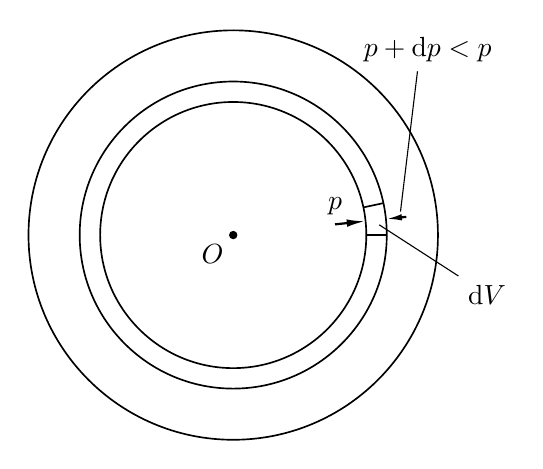
\begin{tikzpicture}[scale=1.3]
			\draw[semithick] (0,0) circle (2);
			\draw[semithick] (0,0) circle (1.3);
			\draw[semithick] (0,0) circle (1.5);
			\filldraw (0,0) circle (1pt);
			\draw[semithick] (0:1.3) -- (0:1.5);
			\draw[semithick] (12:1.3) -- (12:1.5);
			\draw[thick,-{Latex[length=2pt 6,width'=0pt 0.4]}] (6:1) -- (6:1.3);
			\draw[thick,-{Latex[length=1pt 6,width'=0pt 0.4]}] (6:1.7) -- (6:1.5);
			\node[below left] (O) at (0,0) {$O$};
			\node[above] (p) at (6:1) {$p$};
			\draw (8:1.65) -- (1.8,1.6);
			\node[above] (dp) at (1.9,1.6) {$p+\dd{p}<p$};
			\draw (4:1.43) -- (2.2,-0.4);
			\node[below right] (dV) at (2.2,-0.4) {$\dd{V}$};
		\end{tikzpicture}
		\caption{正文图 9-8}\label{pic-9-9-8}
	\end{figure}

	\begin{jie}
		如图~\ref{pic-9-9-8},取厚度 $\dd{r}$ 的球壳上截面积为 $\dd{S}$ 的体积元 $\dd{V} = \dd{r} \dd{S}$,则由受力平衡知
		\begin{gather*}
			p \dd{S} = (p+\dd{p}) \dd{S} + \frac{1}{r^2} m(r) \rho \dd{V},\\
			\implies \dd{p} \dd{S} = - \frac{1}{r^2} m(r) \rho \dd{V},\\
			\implies \dv{p}{r} = - \frac{1}{r^2} m(r) \rho.
		\end{gather*}
	\end{jie}

	\item 试证 OV 流体静力学平衡方程可改写为
	\begin{equation*}
		\left[ 1- \frac{2m(r)}{r} \right]^{1/2} \dv{p}{r} = - \left( \rho + p \right) g, \tag{9-4-60}
	\end{equation*}
	其中 $g$ 代表流体质点的 4 加速 $\tensor{U}{^b} \Nabla{b} \tensor{U}{^a}$ 的大小。

	\begin{yl}{注}
		在牛顿近似下 $\left[ 1 - 2 m(r) / r \right]^{1/2} \cong 1$, $p \cong 0$, 式 (9-4-60) 成为 $\dv*{p}{r} \cong - \rho g$。而 $g \cong m(r)/r^2$,故得式 (9-3-18),即 $\dv*{p}{r} \cong - \rho m(r)/r^2$。
	\end{yl}

	\begin{zm}
		由于 $\tensor{U}{^a} = \e{-A} \tensor{\left( \pdv*{t} \right)}{^a}$,有
		\begin{align*}
			\tensor{U}{^b} \tensor{\nabla}{_b} \tensor{U}{^a} &= \tensor{U}{^b} \tensor{\left( \pdv{t} \right)}{^a} \Nabla{b} \e{-A} + \e{-2A} \tensor{\left( \pdv{t} \right)}{^b} \Nabla{b} \tensor{\left( \pdv{t} \right)}{^a}\\
			&= 0 + \e{-2A} \ChristoffelSymbol{\mu}{0}{0} \tensor{\left( \pdv{x^\mu} \right)}{^a}\\
			&= \dv{A}{r} \e{-2B} \tensor{\left( \pdv{r} \right)}{^a}\\
			&= \left( 1- \frac{2m(r)}{r} \right) \dv{A}{r} \tensor{\left( \pdv{r} \right)}{^a}\\
			&= \frac{r - 2m(r)}{r} \frac{m(r) + 4 \pi p r^3}{r \left( r - 2 m(r) \right)} \tensor{\left( \pdv{r} \right)}{^a}\\
			&= \frac{m(r) + 4 \pi p r^3}{r^2} \tensor{\left( \pdv{r} \right)}{^a},
		\end{align*}
		故
		\begin{align*}
			g &= \sqrt{\tensor{g}{_1_1} \left( \frac{m(r) + 4 \pi p r^3}{r^2} \right)^2}\\
			&= \left( 1 - \frac{2 m(r)}{r} \right)^{-1/2} \frac{m(r) + 4 \pi p r^3}{r^2},
		\end{align*}
		于是
		\begin{align*}
			\left( 1 - \frac{2 m(r)}{r} \right)^{1/2} \dv{p}{r} &= - \left( 1 - \frac{2 m(r)}{r} \right)^{1/2} \left( \rho + p \right) \frac{m(r) + 4 \pi p r^3}{r^2 \left( 1 - \frac{2 m(r)}{r} \right)}\\
			&= - \left( 1 - \frac{2 m(r)}{r} \right)^{-1/2} \left( \rho + p \right) \frac{m(r) + 4 \pi p r^3}{r^2}\\
			&= - \left( \rho + p \right) g.
		\end{align*}
	\end{zm}

	\item 试证当 $R \gg M$ 时式 (9-3-26) 近似回到牛顿引力论的式 (9-3-23)。

	\begin{zm}
		当 $M/R \rightarrow 0$ 时,
		\begin{align*}
			p_0 &= \rho \frac{1- \left( 1 - 2 M/R \right)^{1/2}}{3\left( 1- 2 M/R \right)^{1/2} - 1}\\
			&\sim \rho \frac{1 - \left( 1 - M/R \right)}{2}\\
			&= \frac{\rho}{2 R} M\\
			&= \frac{\rho}{2 R} \frac{4}{3} \pi R^3 \rho\\
			&= \frac{2}{3} \pi \rho^2 R^2.
		\end{align*}
	\end{zm}

	\item 求闵氏时空中 Rindler 坐标 $t,x$ 与洛伦兹坐标 $T,X$ 的关系。

	\begin{jie}
		\begin{align*}
			T &= \frac{U+V}{2}\\
			&= \frac{\e{v} - \e{-u}}{2}\\
			&= \frac{x \e{t} - x \e{-t}}{2}\\
			&= x \sinh{t},\\
			X &= \frac{V - U}{2}\\
			&= \frac{\e{v} + \e{-u}}{2}\\
			&= \frac{x \e{t} + x\e{-t}}{2}\\
			&= x \cosh{t},
		\end{align*}
		反解得
		\begin{align*}
			t &= \tanh^{-1} \frac{T}{X},\\
			&= \frac{1}{2} \ln \frac{X + T}{X - T},\\
			x &= \sqrt{X^2 - T^2}.
		\end{align*}
	\end{jie}

	\item Rindler 时空的类时 Killing 矢量场 $\tensor{\left( \pdv*{t} \right)}{^a}$ 是闵氏时空的哪个 Killing 矢量场?

	\begin{jie}
		由上题得
		\begin{align*}
			\tensor{\left( \pdv{t} \right)}{^a} &= \pdv{T}{t} \tensor{\left( \pdv{T} \right)}{^a} + \pdv{X}{t} \tensor{\left( \pdv{X} \right)}{^a}\\
			&= x \cosh{t} \tensor{\left( \pdv{T} \right)}{^a} + x \sinh{t} \tensor{\left( \pdv{X} \right)}{^a}\\
			&= X \tensor{\left( \pdv{T} \right)}{^a} + T \tensor{\left( \pdv{X} \right)}{^a},
		\end{align*}
		这是 boost 矢量场。事实上,这个矢量场在正文 (4-3-3) 出现过了。
	\end{jie}

	\item 求施瓦西时空中静态观者的 4 加速的长度 $A = \left( \tensor{A}{^a} \tensor{A}{_a} \right)^{1/2}$ 。提示:可借用\hyperlink{prob-8.3}{第 8 章习题 3} 的结论,即 $\tensor{A}{_a} = \Nabla{a} \ln{\chi}$。

	\begin{jie}
		对施瓦西时空,$\tensor{\xi}{^a} = \tensor{\left( \pdv*{t} \right)}{^a}$,
		\begin{equation*}
			\chi = \sqrt{- \tensor{\xi}{_a} \tensor{\xi}{^a}} = \sqrt{1 - \frac{2M}{r}},
		\end{equation*}
		知
		\begin{align*}
			\tensor{A}{_a} &= \Nabla{a} \ln{\chi}\\
			&= \frac{1}{2} \Nabla{a} \ln(1 - \frac{2M}{r})\\
			&= \frac{1}{2} \left( 1 - \frac{2M}{r} \right)^{-1} \Nabla{a} \left( 1 - \frac{2M}{r} \right)\\
			&= \left( 1 - \frac{2M}{r} \right)^{-1} \frac{M}{r^2} \tensor{\left( \dd{r} \right)}{_a},
		\end{align*}
		故
		\begin{align*}
			A &= \sqrt{\tensor{g}{^a^b} \tensor{A}{_a} \tensor{A}{_b}}\\
			&= \left( 1 - \frac{M}{r^2} \right)^{-1} \frac{2M}{r} \sqrt{\tensor{g}{^1^1}}\\
			&= \left( 1 - \frac{M}{r^2} \right)^{-1/2} \frac{2M}{r}.
		\end{align*}
		吐槽:这不是 (8-3-23) 算过的么……
	\end{jie}
\end{xiti}

	% !TeX root = ../document.tex

\chapter{宇宙论}

	\part{中册}
	% !TeX root = ../document.tex

\chapter{时空的整体因果结构}

\begin{xiti}
    \item 试证命题 11-1-10.

    \begin{zm}
        \begin{enumerate}
            \item $\subset$ 的证明:设 $p \in \I^+[\I^+(S)]$,则存在 $q \in \I^+[S] $,使得 $p \in \I^+(q)$;而 $q \in \I^+ [S]$ 意味着存在 $r \in S$ 使得 $q \in \I^+ (r)$,根据“$I+I=I$”,知 $p \in \I^+(r)$,于是 $p \in \I^+(S)$。
            \item $\supset$ 的证明:设 $p \in \I^+(S)$,则存在 $q \in S$ 使得 $p \in \I^+(q)$ ,于是在 $pq$ 间存在一条类时曲线,在其上任取 $r$ ,于是 $r \in \I^+(q)$ 且 $p \in \I^+(r)$,于是 $p \in \I^+[\I^+(S)]$。
        \end{enumerate}
    \end{zm}

    \item 试证命题 11-1-11(c)。提示:利用 $A \subset B \implies \ii{A} \subset \ii{B}$。

    \begin{zm}
        \begin{enumerate}
            \item $\subset$ 的证明:由定义,$\I^+(S) \subset \J^+ (S)$,于是 $\I^+(S) = \ii{\I^+ (S)} \subset \ii{\J^+(S)}$。
            \item $\supset$ 的证明:设 $p \in \ii{\J^+(S)}$,则意味着存在 $p$ 的邻域 $O$ 使 $O \subset \J^+(S)$。取 $q \in O \cap \I^-(p)$ ,则 $O \subset \J^+(S)$ 意味着存在 $r \in S$ 使得 $q\in \J^+(r)$ ,于是由“$J + I = I$” 知 $p \in \I^+(r)$,故 $p \in \I^+(S)$ 。
        \end{enumerate}

        \paragraph{注} 可能会以为利用命题 11-1-11(b) 两边取内部可以直接推出命题 11-1-11(c)。(至少我这么以为过……)然而 $\ii{A}$ 和 $\ii{\bar{A}}$ 未必相同。例如,一个极端的例子是取 $A$ 为 $\left(\mathbb{R}^n,\TT_u\right)$ 中全体有理点的集合(即 $\mathbb{Q}^n$),则 $\ii{A}= \varnothing$,而 $\bar{A}$ 和 $\ii{\bar{A}}$ 是整个 $\mathbb{R}^n$!即使限制 $A$ 为开集也无济于事,例如在 $(\mathbb{R},\TT_u)$ 中令 $A = (a,b) \cup (b,c)$,则 $\bar{A} = [a,c]$,显然它们的内部不相同。
    \end{zm}

    \item 由时空背景流形的 $T_2$ 性出发按 \S 11.2 定义1证明任一指向未来因果线最多有一个未来端点。

    \begin{zm}
        设指向未来因果线 $\gamma(t) \colon I \rightarrow M$ 有两个未来端点 $p$ 和 $q$,则由于时空的 $T_2$ 性,存在 $p$ 的一个邻域 $A$ 和 $q$ 的一个邻域 $B$ 使得 $A\cap B = \varnothing$。而根据未来端点的定义,存在 $t_1 \in I$ 使得 $\forall t \in I,t > t_1$ 有 $\gamma(t) \in A$;以及存在 $t_2 \in I$ 使得 $\forall t \in I,t > t_2$ 有 $\gamma(t) \in B$。于是若取 $t_3 \in I , t>\max\{t_1,t_2\}$,则 $\gamma(t_3)\in A \cap B$,矛盾。于是未来端点最多有一个。
    \end{zm}

    \item 下列5个都是貌似正确的伪命题。试用对闵氏时空挖空和认同的手法各举一反例以否定之[见 Geroch and Horowize(1979)]。
    \begin{enumerate}
        \item[(a)] $q\in \dot{\I}^-(p) \implies $ 从 $q$ 出发的躺在 $\dot{\I}^-(p)$ 上的指向未来类光测地线必到达 $p$。
        \item[(b)] $\I^-(q) \subset \I^-(p) \implies \I^+(p) \implies \I^+(q) $。提示:从2维闵氏时空挖去 $x$ 轴的一段使 $\I^+(q)$ “小”到连与$\I^+(p)$ 相交都不可能。
        \item[(c)] $\I^-(p) = \I^-(q) \implies p = q$。提示:借用图 11-4.
        \item[(d)] $q \notin \I^-(p) \implies \exists $ 起自 $q$ 的永不进入 $\I^-(p)$ 的过去不可延因果线。[提示:从2维闵氏时空挖去一直线段使 $q \in \dot{\I}^-(p)$。]
        \item[(e)] $q \in \dot{\I}^+(p) \cap \dot{\I}^-(p) \implies q=p$。提示:见 Geroch and Horowize(1979) 。
    \end{enumerate}

    \begin{jie}
        \begin{enumerate}
            \item[(a)] 在连接 $pq$ 的直线段(这是一条类光测地线)上挖去一点即可。
            \item[(b)] 如图
        \end{enumerate}
    \end{jie}
\end{xiti}
	\chapter*{附录B \quad 量子力学数学基础简介}
\addcontentsline{toc}{chapter}{附录B    量子力学数学基础简介}
\setcounter{xiti}{0}

\begin{xiti}
    \item 设 V 是内积空间,它(作为矢量空间)的零元记作0,试证 $ (0,g)=0 \in \mathbb{C} \quad \forall g \in V. $

    \begin{zm}
        由内积的线性性,$\forall f,g \in V$,
        \begin{equation*}
            (f,g) = (f+0,g) = (f,g) + (0,g),
        \end{equation*}
        这表明 $(0,g)$ 是数域 $\mathbb{C}$ 的零元。
    \end{zm}

    \item 验证用式 (B-1-1) 定义的 $(f,g)$ 满足内积定义(\S B.1 定义1)的4个条件。

    \begin{zm}
        式 B-1-1:
        \begin{equation*}
            (f,g) := \int_a^b \overline{f(x)} g(x) \dd{x} \qc \forall f,g \in C[a,b].
        \end{equation*}
    \end{zm}
\end{xiti}
	\chapter*{附录G \quad 李群和李代数}
\addcontentsline{toc}{chapter}{附录G\quad 李群和李代数}
\setcounter{xiti}{0}
\begin{xiti}
	\item 验证由式(G-1-1)定义的$I_g \colon G\rightarrow G$确为自同构映射。
	
	\begin{zm}
		$I_g $定义为
		\[I_g(h) := g h g^{-1}\qc \forall g\in G, \]
		首先验证它是同态:
		\begin{displaymath}
		I_g (h_1 h_2) = g h_1 g^{-1} g h_2 g^{-1}= g h_1 h_2 g^{-1} = I_g (h_1 h_2),
		\end{displaymath}
		而
		\begin{displaymath}
		I_{g^{-1}} (I_g (h) )= g^{-1} \left( g h g^{-1} \right) g=h
		\end{displaymath}
		故$I_g $有逆映射$I_{g_{-1}} $,于是$I_g $是自同构映射。
	\end{zm}
	
	\item 验证由式(G-1-2)定义的乘法满足群乘法的要求。
	
	\begin{zm}
		\begin{enumerate}
			\item 结合律:
			\begin{displaymath}
			\left( \left(g_1,g^\prime_1\right) \left(g_2,g^\prime_2\right) \right) \left(g_3,g^\prime_3\right) = \left( g_1 g_2 g_3 , g^\prime_1 g^\prime_2 g^\prime_3 \right)= \left( g_1,g^\prime_1 \right) \left( \left( g_2,g^\prime_2 \right) \left( g_3,g^\prime_3 \right) \right) 
			\end{displaymath}
			\item 含幺:
			\begin{displaymath}
			\left( e,e^\prime \right) \left( g,g^\prime \right) = \left( g,g^\prime \right) = \left( g,g^\prime \right)
			\end{displaymath}
			\item 有逆:
			\begin{displaymath}
			\left( g,g^\prime \right) \left( g^{-1}, {g^\prime}{_1} \right)= \left( e,e^\prime \right)
			\end{displaymath}
		\end{enumerate}
	\end{zm}

    \item 验证由\S G.1 定义 8 所定义的 $A(G) $是群。
    
    \begin{zm}
    	\begin{enumerate}
    		\item 先验证复合确实是$A(G) $上的运算$\circ\colon A(G)\times A(G) \rightarrow A(G) $,即$\forall \mu,\nu \in A(G) $,验证$\mu \circ \nu \in A(G) $:
    		首先验证$\mu\circ \nu $是同态:\[ \mu\circ \nu (gh)=\mu\left( \nu(g) \nu(h) \right) =\mu\circ \nu (g) \mu\circ \nu(h), \]
    		再验证$\mu\circ \nu $一一到上(有逆映射):\[ \left(\mu\circ \nu\right) \circ \left(\nu^{-1} \circ \mu^{-1}\right) = \operatorname{Id}_G, \]
    		故$\mu\circ\nu $有逆映射$\nu^{-1} \circ \mu^{-1} $,于是$\mu\circ\nu$为同构映射,故复合是$A(G)$上的运算。
    		\item 验证$\circ$为群乘法:
    		\begin{enumerate}
    			\item 结合律:\[ \mu \circ \left( \nu \circ \sigma \right) =\mu \circ \nu \circ \sigma = \left( \mu \circ \nu \right) \circ \sigma\qc \forall \mu,\nu,\sigma \in A(G). \]
    			\item 含幺:易知$\operatorname{Id}_G \in A(G) $,\[ \operatorname{Id}_G \circ \mu = \mu \circ \operatorname{Id}_{G} = \mu\qc \forall \mu \in A(G) \]
    			\item 有逆:$\forall \mu \in A(G) $,$\mu^{-1}$也是自同构,于是\[ \mu \circ \mu^{-1} = \mu^{-1} \circ \mu = \operatorname{Id}_G. \]
    		\end{enumerate}
    	\end{enumerate}
    \end{zm}

    \item 试证定理G-1-2,即$A_I(G)$是群$A(G)$的正规子群。
    
    \begin{zm}
    	$\forall \mu \in A(G),I_g\in A_I(G),h\in G $,\[ \mu\circ I_g \circ \mu^{-1} (h) =\mu \left( g (\mu^{-1} h) g^{-1} \right) = \mu(g) h \mu(g)^{-1} = I_{\mu(g)}(h) . \]
    \end{zm}
    
    \item 验证由\S G.1 定义9所定义的$H \otimes_S K $是群。
    
    \begin{zm}
    	\begin{enumerate}
    		\item 结合律:$\forall h_1 , h_2 , h_3 \in H , k_1 , k_2 , k_3 \in K $,
    		\begin{align*}
    		\left( (h_1,k_1) (h_2,k_2) \right) (h_3 , k_3) &= \left(h_1 \mu_{k_1}(h_2), k_1 k_2 \right) (h_3,k_3)\\
    		&= \left( h_1 \mu_{k_1}(h_2) \mu_{k_1 k_2}(h_3) , k_1 k_2 k_3 \right)\\
    		&= \left( h_1 \mu_{k_1}(h_2) \mu_{k_1}\left( \mu_{k_2}(h_3) \right)  , k_1 k_2 k_3 \right)\\
    		&= \left( h_1 \mu_{k_1}(h_2 \mu_{k_2}(h_3)) , k_1 k_2 k_3 \right)\\
    		&= (h_1,k_1) \left( h_2 \mu_{k_2}(h_3) , k_2 k_3 \right)\\
    		&= (h_1,k_1) \left( (h_2,k_2) (h_3,k_3) \right)
    		\end{align*}
    		\item 含幺:$\forall h \in H, k\in K $,
    		\[ (e_H,e_K) (h,k) = (h,k) = (h,k) (e_H,e_K) \]
    		\item 有逆:$\forall h \in H,k \in K $,
    		\[ (h,k) (h^{-1},k^{-1}) = (e_H,e_K) = (h^{-1} ,k^{-1}) (h,k) \]
    	\end{enumerate}
    \end{zm}
	
	\item 设$L_g \colon G \rightarrow G $是由$g\in G $生成的左平移,${L_g}^{-1} $是$L_g$的逆映射,试证\[ L_{g^{-1}} = {L_g}^{-1}\qc \forall g\in G. \]
	
	\begin{zm}
		$\forall h\in G $,
		\[ L_{g^{-1}} \left(L_g(h)\right) = g^{-1} gh=h, \]
		故$L_{g^{-1}} \circ L_{g} =\operatorname{Id}_G $。
	\end{zm}
	
	\item $\forall g \in G $定义右平移$ R_g \colon h \mapsto hg \qc{\forall h \in G} $,试证$R_{gh} = R_{h} \circ R_g $。
	
	\begin{zm}
		$\forall g,h,k\in G$,\[ R_{gh}(k) = kgh=R_{h}\circ R_g (k) \]
	\end{zm}
    
    \item 试证$[\myvec{v},\myvec{u}]:= \myvec{v} \cp \myvec{u} \qc \forall \myvec{v} ,\myvec{u} \in \mathbb{R}^3 $满足李括号的条件(见\textsection G.3 例 1 )。
    
    \begin{zm}
    	线性性、反称性易知。验证雅可比恒等式:
    	\begin{align*}
    	&\tmu \left[\myvec{u},\left[\myvec{v},\myvec{w}\right]\right] + \left[\myvec{v},\left[\myvec{w},\myvec{u}\right]\right] + \left[\myvec{w},\left[\myvec{u},\myvec{v}\right]\right]\\
    	=&\;\myvec{u} \cp \left( \myvec{v} \cp \myvec{w} \right) + \myvec{v} \cp \left( \myvec{w} \cp \myvec{u} \right) + \myvec{w} \cp \left( \myvec{u} \cp \myvec{v} \right)\\
    	=&\tmu\left(\myvec{u} \vdot \myvec{w}\right) \myvec{v} - \left(\myvec{u} \vdot \myvec{v}\right) \myvec{w} + \left(\myvec{v} \vdot \myvec{u}\right) \myvec{w} - \left(\myvec{v} \vdot \myvec{w}\right) \myvec{u} + \left(\myvec{w} \vdot \myvec{u}\right) \myvec{v} - \left(\myvec{w} \vdot \myvec{v}\right) \myvec{u}\\
    	=&\;0,
    	\end{align*}
    	其中三矢量叉乘可以这样得到:叉乘 $\tensor[^*]{\left(\bm{u}\wedge\bm{v}\right)}{}$ 用体元表达为 $\tensor{\varepsilon}{_a_b_c} \tensor{u}{^a} \tensor{v}{^b}$ ,于是
    	\begin{displaymath}
    	\tensor{\varepsilon}{_a_b_c} \tensor{u}{^a} \tensor{\varepsilon}{^d^e^b} \tensor{v}{_d} \tensor{w}{_e} = 2 \tensor{\delta}{^{[a}_e} \tensor{\delta}{^{c]}_d} \tensor{u}{^a} \tensor{v}{_d} \tensor{w}{_e} = \tensor{u}{^a} \tensor{w}{_a} \tensor{v}{_c} - \tensor{u}{^a} \tensor{v}{_a} \tensor{w}{_c}.
    	\end{displaymath}
    \end{zm}

    \item 试证 $\left[A,B\right] := AB-BA$ 满足李括号的条件(见 \S G.3 例2)。
    
    \begin{zm}
    	线性性、反称性易知,验证雅可比恒等式:
    	\begin{align*}
    	&\tmu\left[A,\left[B,C\right]\right] + \left[B,\left[C,A\right]\right] + \left[C,\left[A,B\right]\right]\\
    	=&\;A \left(BC-CB\right) - \left(BC-CB\right) A \\
    	&+ B \left(CA-AC\right) - \left(CA-AC\right) B \\
    	&+ C \left(AB-BA\right) - \left(AB-BA\right) C\\
    	=&\;ABC-ACB-BCA+CBA\\
    	&+ BCA-BAC-CAB+ACB\\
    	&+CAB-CBA-ABC+BAC\\
    	=&\;0.
    	\end{align*}
    \end{zm}
    
    \item 设 $\mathscr{G}$ 和 $\hat{\mathscr{G}}$ 依次是李群 $G$ 和 $\hat{G}$ 的李代数,$\rho_* \colon \mathscr{G} \rightarrow \hat{\mathscr{G}}$ 是同态映射 $\rho\colon G\rightarrow \hat{G}$ 在 $e\in G$ 诱导的推前映射,试证 $\rho \left(\exp A\right) = \exp(\rho_* A) \quad \forall A \in \mathscr{G}$。提示:先用同态性证明 $\rho \left(\exp tA\right)$ 是单参子群。
    
    \begin{zm}
    	由同态性,
    	\begin{displaymath}
    	\rho \left(\exp sA\right) \rho \left(\exp tA\right) = \rho \left(\left(\exp sA\right)\left(\exp tA\right)\right) = \rho \left(\exp((s+t)A)\right)
    	\end{displaymath}
    	故 $\rho \left(\exp tA\right)$ 为 $\hat{G}$ 上的单参子群。它在恒等元的切矢为
    	\begin{displaymath}
    	\left.\dv{t} \rho \left(\exp t A\right) \right|_e = \rho_* \left. \dv{t} \exp(tA) \right|_e = \rho_* A
    	\end{displaymath}
    	故 $\rho\left(\exp tA\right)$ 是 $\rho_* A$ 生成的单参子群,即 $\rho\left(\exp tA\right)=\exp(t\rho_* A)$ , 取 $t=1$ 即得要证的等式。
    \end{zm}
	
	\item 试证式 (G-5-10) 可由式 (G-5-10') 推出。提示:把式(G-5-10)的 $\tensor{v}{^a},\tensor{u}{^a}$ 之和作为式 (G-5-10') 的 $\tensor{v}{^a}$ 。
	
	\begin{zm}
		由式(G-5-10'),即
		\begin{displaymath}
		\tensor{g}{_a_b} \left( \tensor{Z}{^a_c} \tensor{v}{^c} \right) \left( \tensor{Z}{^b_d} \tensor{v}{^d} \right) = \tensor{g}{_c_d} \tensor{v}{^c} \tensor{v}{^d} \qc \forall \tensor{v}{^c} \in V
		\end{displaymath}
		则任取 $\tensor{u}{^a},\tensor{v}{^a}\in V$,有
		\begin{displaymath}
		\tensor{g}{_a_b} \left( \tensor{Z}{^a_c} \left( \tensor{u}{^c} + \tensor{v}{^c} \right) \right) \left( \tensor{Z}{^b_d} \left( \tensor{u}{^d} + \tensor{v}{^d} \right) \right) = \tensor{g}{_c_d} \left( \tensor{u}{^c} + \tensor{v}{^c} \right) \left( \tensor{u}{^d} + \tensor{v}{^d} \right)
		\end{displaymath}
		左边展开为
		\begin{align*}
		&\;\tensor{g}{_a_b} \left( \tensor{Z}{^a_c} \tensor{u}{^c} \right) \left( \tensor{Z}{^b_d} \tensor{u}{^d} \right) + \tensor{g}{_a_b} \left( \tensor{Z}{^a_c} \tensor{v}{^c} \right) \left( \tensor{Z}{^b_d} \tensor{v}{^d} \right) + 2 \tensor{g}{_a_b} \left( \tensor{Z}{^a_c} \tensor{u}{^c} \right) \left( \tensor{Z}{^b_d} \tensor{v}{^d} \right)\\
		=&\;\tensor{g}{_c_d} \tensor{u}{^c} \tensor{u}{^d} +  \tensor{g}{_c_d} \tensor{v}{^c} \tensor{v}{^d} + \color{blue} 2 \tensor{g}{_a_b} \left( \tensor{Z}{^a_c} \tensor{u}{^c} \right) \left( \tensor{Z}{^b_d} \tensor{v}{^d} \right)
		\end{align*}
		右边展开为
		\begin{align*}
		 \tensor{g}{_c_d} \tensor{u}{^c} \tensor{u}{^d} + \tensor{g}{_c_d} \tensor{v}{^c} \tensor{v}{^d} + \color{blue} 2 \tensor{g}{_c_d} \tensor{u}{^c} \tensor{v}{^d}
		\end{align*}
		蓝色部分相等即给出式(G-5-10)。
	\end{zm}
	
	\item $\mathrm{SO}(2)$ 是阿贝尔群吗?$\mathrm{O}(2)$ 是阿贝尔群吗?
	
	\begin{da}
		是;不是。
	\end{da}
	
	\item 李群 $\mathrm{SL}(m)$ [ $\mathrm{GL}(m)$ 满足 $\det T=+1$ 的子群 ] 的李代数记作 $\mathscr{S\!\!L}(m)$ 。试证
	\begin{displaymath}
	\text{(a)}\;\mathscr{S\!\!L}(m)=\{ m\times m \text{无迹实矩阵} \} \qc\quad \text{(b)}\;\dim \mathrm{SL}(m)=m^2-1.
	\end{displaymath}
    
    \begin{zm}
    	\begin{enumerate}
    		\item[(a)] 回忆引理(G-5-12),
    		\begin{yl}{Lm}
    			$\det(\Exp A)=\e{\tr A}\qc \forall A\in \mathscr{M}(m)$
    		\end{yl}
    	    设 $T(t)$ 是 $\mathrm{SL}(m)$ 上的曲线,且 $T(0)=I$ 为恒等映射。其在 $I$ 的切矢的分量为
    	    \begin{displaymath}
    	    \tensor{A}{^\mu_\nu} = \left. \dv{t} \tensor{T}{^\mu_\nu}(t) \right|_0
    	    \end{displaymath}
    	    或者写成矩阵等式\footnote{注意分量形式中左边 $\tensor{A}{^\mu_\nu}$ 是切矢在坐标基下的分量,而右边的 $\tensor{T}{^\mu_\nu}$ 却是流形上点的坐标,从分量写成矩阵配的并不是同一组基,这样看来写成矩阵等式显得很令人困惑。不过,如果将矩阵和线性变换严格区分,从而认为矩阵不过是一堆数,那么只要声明了矩阵是在哪个基下的矩阵(比如这里是不言自明的),那么将切矢写作矩阵求导就一点问题也没有。}
    	    \begin{displaymath}
    	    A=\left. \dv{t} T(t) \right|_0
    	    \end{displaymath}
    	    \begin{enumerate}[leftmargin=2em]
    	    	\item[i.] $\forall A\in \mathscr{S\!\!L}(m)$ ,有 $\Exp(A) = \exp(A) \in \mathrm{SL}(m)$ ,取行列式即有
    	    	\begin{align*}
    	    	\e{\tr A} = \det(\Exp A) = 1 \implies \tr A=0.
    	    	\end{align*}
    	    	\item[ii.] $\forall A\in \mathscr{M}(m)$ 且 $\tr A=0$ ,要证明 $A\in \mathscr{S\!\!L}(m)$ ,只需考虑 $\Exp(tA)$ ,由于
    	    	\begin{displaymath}
    	    	\det(\Exp(tA)) = \e{t\tr A} = 1,
    	    	\end{displaymath}
    	    	故 $\forall t\in \mathbb{R}\qc \Exp(tA) \in \mathrm{SL}(m)$,而
    	    	\begin{displaymath}
    	    	A=\left. \dv{t} \Exp(tA) \right|_0
    	    	\end{displaymath}
    	    	故 $A$ 是曲线 $\Exp(tA)$ 在 $I$ 的切矢,它是 $\mathscr{S\!\!L}(m)$ 中的元素。
    	    \end{enumerate}
            \item[(b)] 由 $\dim \mathrm{SL}(m) = \dim \mathscr{S\!\!L}(m)$ ,$\mathscr{S\!\!L}(m)$ 中的矩阵有 $m^2$ 个矩阵元,迹为零给出一个方程,则共有 $m^2-1$ 个独立参数,故 \[\dim \mathrm{SL}(m) = \dim \mathscr{S\!\!L}(m)=m^2-1.\]
    	\end{enumerate}
    \end{zm}
	
	\item \begin{enumerate}
		\item[(1)] 试证明存在连续曲线 $\mu \colon [0,1] \rightarrow \mathrm{GL}(2)$ 使 $\mu(0)=I$,$\mu(1)=\mqty(-1 & 1 \\ 0 & -1)$。
		\item[(2)] 试证 $T\equiv \mqty(-1 & 1 \\ 0 & -1) \in \mathrm{GL}(2)$ 不属于李群 $\mathrm{GL}(2)$ 的任一单参子群。提示:假定存在矩阵 $A=\mqty(a&b\\c&d)$ 使 $T=\Exp(A)$,(a) 证明 $c\neq 0$,(b) 把 $A^n$ ($A$ 的 $n$ 次方)记作 $A^n \equiv \mqty(a_n & b_n \\ c_n & d_n)$ ,证明 $\exists r_n\in \mathbb{R}$ 使 $b_n = b r_n$ , $c_n=c r_n$。(c) 由 (b) 推出矛盾。
	\end{enumerate}
    
    \begin{zm}
    	\begin{enumerate}
    		\item[(1)] 令
    		\begin{displaymath}
    		\mu(t) := \mqty(1-2t & t \\ 0 & 1-2t)\qc \forall t\in [0,1]
    		\end{displaymath}
    		则
    		\begin{displaymath}
    		\det \mu(t) = \left(1-2t\right)^2 -0 \neq 0 \implies \mu(t) \in \mathrm{GL}(2).
    		\end{displaymath}
    		$\mu(t)$是满足要求的曲线。
			\item[(2)] 假设存在 $A=\mqty(a & b \\ c & d)$ 使得 $T=\Exp(A)$,则若 $c=0$,我们用数学归纳法证明 $A^n=\mqty(a^n & x_n \\ 0 & d^n)$,其中 $x_n$ 是含 $a,b,d$ 的多项式:
			\begin{enumerate}
				\item $n=1$ 时,命题成立;
				\item 设 $n=k$ 时命题成立,则 $A^{k+1}=A A^k= \mqty(a^{k+1} & a x_k + b d^k \\ 0 & d^{k+1})$,故命题成立。
			\end{enumerate}
			于是 $A^n=\mqty(a^n & x_n \\ 0 & d^n)$ 得证。由此易得 $\Exp(A)=\mqty(\exp(a) & x \\ 0 & \exp{d})$ ,而$\exp(a)=-1$ 无实数解,矛盾。
    	\end{enumerate}
    \end{zm}
	
\end{xiti}

	\backmatter
	\printbibliography
\end{document}
